\documentclass[12pt]{report}

% GENERAL PACKAGES
\usepackage{geometry} % sets the parameters of the page
\usepackage{tgpagella} % changed the font, still not great
\usepackage{natbib} % bibliography
\usepackage{hyperref} % for the references
\usepackage[bottom]{footmisc} % moves footnotes below figures
\geometry{letterpaper, portrait, margin=1.25in}
\usepackage{multirow} % for several rows in the same cell
\usepackage{fontawesome} % for those pretty icons
\usepackage{tcolorbox}
\usepackage{xcolor}
\usepackage{colortbl}
\usepackage{bm} % bold math mode
\usepackage{esvect} % arrows above text
\usepackage[titletoc]{appendix}

% DESIGN RELATED STUFF
\usepackage{tikz} % automata, trees, etc.
\usetikzlibrary{automata,positioning,arrows.meta}
\usetikzlibrary{decorations.pathmorphing}
\usetikzlibrary{decorations.pathreplacing}
\tikzset{every picture/.style={line width=0.75pt}} %set default line width to 0.75pt   
\usepackage{amsmath} % text encoding of transitions
\usepackage{amssymb} % \ltimes and \rtimes
\usepackage{amsthm} % for theorems
\newtheorem{thm}{Theorem}
\usepackage{algorithm} % for pseudocodes
\usepackage{algorithmic} % for pseudocodes
\usepackage{arydshln} % for dashed lines in tables
%\theoremstyle{definition}
%\newtheorem{definition}{Definition}[section]
\newtheoremstyle{mystyle}%                % Name
  {}%                                     % Space above
  {}%                                     % Space below
  {\itshape}%                                     % Body font
  {}%                                     % Indent amount
  {\bfseries}%                            % Theorem head font
  {\\}%                                    % Punctuation after theorem head
  { }%                                    % Space after theorem head, ' ', or \newline
  {}%                                     % Theorem head spec (can be left empty, meaning `normal')

\theoremstyle{mystyle}
\newtheorem{definition}{Definition}[section]
\usepackage{dashbox} % for dashed boxes
\newcommand\dboxed[1]{\dbox{\ensuremath{#1}}}




\usepackage{placeins} % allows to use \FloatBarrier

%\usepackage{graphicx,kantlipsum,setspace}
%\usepackage{setspace}
%\usepackage{caption} % special spacings for tables and figures
%\captionsetup[table]{font={stretch=1}}
%\captionsetup[figure]{font={stretch=1}}

\usepackage{amsmath}
\usepackage{tikz}
\usepackage{mathdots}
\usepackage{yhmath}
\usepackage{cancel}
\usepackage{color}
\usepackage{siunitx}
\usepackage{array}
\usepackage{multirow}
\usepackage{amssymb}
\usepackage{gensymb}
\usepackage{tabularx}
\usepackage{booktabs}
\usetikzlibrary{fadings}
\usetikzlibrary{patterns}
\usetikzlibrary{shadows.blur}
\usetikzlibrary{shapes}

%\usepackage[font=singlespacing]{caption}


% LINGUISTICS
\usepackage{tipa} % for IPA characters

\newcommand{\bow}{\ensuremath{\rtimes}} % initial edge
\newcommand{\eow}{\ensuremath{\ltimes}} % final edge

\newcommand{\alena}[1]{{\color{green!60!black}#1}} % for internal speech

% CODE SNIPPETS
\usepackage{listings}

\definecolor{codegreen}{rgb}{0,0.6,0}
\definecolor{codegray}{rgb}{0.5,0.5,0.5}
\definecolor{codepurple}{rgb}{0.58,0,0.82}
\definecolor{backcolour}{rgb}{0.95,0.95,0.92}

\lstdefinestyle{mystyle}{
    backgroundcolor=\color{backcolour},   
    commentstyle=\color{codegreen},
    keywordstyle=\color{magenta},
    numberstyle=\tiny\color{codegray},
    stringstyle=\color{codepurple},
    basicstyle=\ttfamily\footnotesize,
    breakatwhitespace=false,         
    breaklines=true,                 
    captionpos=b,                    
    keepspaces=true,                 
    numbers=left,                    
    numbersep=5pt,                  
    showspaces=false,                
    showstringspaces=false,
    showtabs=false,                  
    tabsize=2
}

\lstset{style=mystyle}

\makeatletter
\def\new@fontshape{}
\makeatother
\usepackage{gb4e} % for linguistic examples: NEEDS TO BE THE LAST
\noautomath
\linespread{1.5}

% the 4 lines below turn off hyphenation
\tolerance=1
\emergencystretch=\maxdimen
\hyphenpenalty=10000
\hbadness=10000


\begin{document}

\pagenumbering{roman}

% -------------------------------------------------------

%% TITLE PAGES
% ========== TITLE PAGE BEGINS ==========
%

\begin{center}
\thispagestyle{empty}

\textcolor{white}{.} \\
\vspace{3em}

{

\textbf{Tool-assisted induction of subregular languages and mappings} \\
\vspace{3em}

A Dissertation Presented \\ \vspace{1em}
by \\ \vspace{1em}
\textbf{Al\"ena Aks\"enova} \\ \vspace{1em}
to \\ \vspace{1em}
The Graduate School \\ \vspace{1em}
in Partial Fulfillment of the \\ \vspace{1em}
Requirements \\ \vspace{1em}
for the Degree of \\ \vspace{1em}
\textbf{Doctor of Philosophy} \\ \vspace{1em}
in \\ \vspace{1em}
\textbf{Linguistics} \\
\vspace{5em}

Stony Brook University \\
\vspace{2em}

\textbf{May 2020}
}
\end{center}



\newpage



\begin{center}
\textbf{Stony Brook University} \\ \vspace{2em}
The Graduate School \\ \vspace{2.3em}
\textbf{Al\"ena Aks\"enova} \\ \vspace{2.3em}
We, the dissertation committee or the above candidate for the \\
Doctor of Philosophy degree, hereby recommend \\
acceptance of this dissertation \\ \vspace{2.3em}
\textbf{Thomas Graf -- Dissertation Advisor} \\
\textbf{Professor, Department of Linguistics}  \\ \vspace{2.3em}
\textbf{Mark Aronoff -- Chairperson of Defense} \\
\textbf{Professor, Department of Linguistics}  \\ \vspace{2.3em}
\textbf{Jeffrey Heinz} \\
\textbf{Professor, Department of Linguistics}  \\ \vspace{2.3em}
\textbf{Richard William Sproat} \\
\textbf{Senior Staff Research Scientist, Google}  \\ \vspace{2.3em}
This dissertation is accepted by the Graduate School \\ \vspace{2.3em}
Eric Wertheimer \\
Dean of the Graduate School
\end{center}
\newpage


% ABSTRACT
\begin{center}
Abstract of the Dissertation \\ \vspace{1em}
\textbf{Tool-assisted induction of subregular languages and mappings} \\ \vspace{1em}
by \\ \vspace{1em}
\textbf{Al\"ena Aks\"enova} \\ \vspace{1em}
\textbf{Doctor of Philosophy} \\ \vspace{1em}
in \\ \vspace{1em}
\textbf{Linguistics} \\ \vspace{1em}
Stony Brook University \\ \vspace{1em}
\textbf{2020} \\ \vspace{3em}
\end{center}



The last decade was very fruitful in the field of subregular research.
New classes of subregular languages and mappings were uncovered for modeling natural language phenomena, and new learning algorithms were developed for these classes.
The subregular approach has been successfully applied to phonotactics \citep{Heinz10ldp}, rewrite processes in phonology and morphology \citep{Chandlee2014}, and even syntactic constraints over tree structures \citep{Graf18CLS}.
However, the rapid pace of the theoretical research has not been matched when it comes to engineering considerations.
Many of the proposed learning algorithms have not been implemented yet, and as a result, their performance on concrete data sets is not known.

In my dissertation, I implement and experiment with some of the learners available for subregular languages and mappings.
I test these learners on data that is modeled after linguistic phenomena such as word-final devoicing and various types of harmony systems.
The code for these evaluations is available as part of my Python package \emph{SigmaPie} \href{https://pypi.org/project/SigmaPie/}{\faCube} \citep{sigmapie}.

The findings of my thesis allow linguists and formal language theorists to assess possible applications of subregular techniques and approaches, in particular typology, cognitive science, and natural language processing.
\newpage


\tableofcontents
\newpage

\cleardoublepage
\addcontentsline{toc}{chapter}{\listfigurename}
\listoffigures
\newpage

\cleardoublepage
\addcontentsline{toc}{chapter}{\listtablename}
\listoftables
\newpage

\addcontentsline{toc}{chapter}{Acknowledgements}
\chapter*{Acknowledgements}
{\small 
For a fun virtual defense, I am grateful to my dissertation committee: Thomas Graf, Mark Aronoff, Jeff Heinz, and Richard Sproat.
Your words of wisdom, comments, and support are precious to me.
A very special thank you I owe to Thomas Graf who was my guide and mentor these five years.
Without your input, I would not be able to make it to this moment.
This route was not easy, but you were always able to understand me and give helpful advice or a good idea, directly and indirectly.
Even when everything seemed worthless, just as many things seem to be worthless when they are difficult, you helped me to keep going.


John Bailyn, without you, I would not be here at Stony Brook.
Only after attending your summer schools in Saint Petersburg, I realized that doing research is not an unbearably fastidious activity, but rather a curious journey.
Sometime in 2014, you told me ``Hey, you should apply to SBU.
We have a new faculty member, Thomas Graf, and you guys might want to work together.''
Although I had not considered applying to Ph.D. before, it somehow sounded like a good idea.
Since then, you were always there for me.

I would never get to know about John Bailyn's summer school without Ekaterina Anatolyevna Lyutikova, my advisor at Moscow State University, and Sergei Georgievich (SG) Tatevosov, our fieldwork boss.
SG once said, ``Ph.D. is the right choice that you will frequently regret.''
Well, now I know what you meant, and thank you for inspiring me to accept this challenge.
I am grateful for all those breathtaking fieldwork trips, that were an unlimited source of material for stories and memories ranging from wild and bizarre to inspiring and life-changing.
Many times I dreamed of staying in those places.

Ph.D. initially felt like a fieldwork experience in better living conditions.
Luckily, this time, I could stay.
SBU linguistic department is indeed a very unique place, where distinguished professors bake the best banana bread, invited speakers show how to Slav squat, and there is frequently an after-party after colloquium receptions, all while doing superb research.
Mark Aronoff, apart from that damn good banana bread, thank you for your wisdom and the ability to share it in a tasteful and fun way.
Lori Repetti, your kindness, ability to explain, and sense of style is something that keeps fascinating and inspiring me.
Bob Hoberman, every meeting we had was twice as long as we expected, because there were just too many exciting things in the world that we needed to discuss, and we could not stop.
Jeff Heinz, you were always there to help and give a piece of sought-for advice, be it life or research.
Andrei Antonenko, you keep blowing my mind with your talents, that go way beyond contagiously energetic teaching and cooking the best steak in the world.
Sandra and Michelle, our department would never work the way it does without you.
Thank you, dear SBU faculty and staff.

During these years, I met some of the brightest people.
Aniello De Santo, we started and ended our Ph.D. journeys at the same time, had the same adviser, and even stayed in the same house all this time.
This was a challenge by itself, considering how different we are, but we managed to make the best out of it and became close friends.
I will miss our evening chats about everything, from silly rumors to the meaning of life, and our anxious pre-defense baking.
The only other person who stayed these whole five years with us in the same house was Sanket Deshmukh.
Sanket, we talked these years non-stop, solved coding challenges together, and I still remember you explaining to me the eight queens puzzle in the basement after drinking the amount of wine that I should not mention in the acknowledgments section of my dissertation.
Thank you for helping me grow.
Ayla Karaka\c{s}, thank you for having my back when even I didn't have it.
I will always remember how we were jumping high at ASOT and Dreamstate, and even higher when you got into Yale's Ph.D. program.
Good luck, bro.
Sophie Moradi, you were always there for me, helping the sun to shine even when it was getting dark.
Hongchen Wu, you are a wonderful example that one can be caring, hard-working, and goofy at the same time.
Nazila Shafiei, thank you for the constant ability to make people around you feel better, it is definitely your talent.
Thank you, Hossep Dolatian, for finding the best in any situation, and for your endless willingness to help.
Jon Rawski, thank you for always having a fun story to share.
No one knows food and drink places in any city of the world better than Chikako Takahashi.
Unfortunately, I need to start wrapping this section up, but I cannot do so without mentioning Sagnik Das, Darius Coelho, Ji Yea Kim, Alex Yeung, Andrija Petrovic, SeoYoung Kim, Ali Salehi, Yaobin Liu, Hyunah Baek, Varya Magomedova, Chong Zhang, Rob Pasternak, So Young Lee, Veronica Miatto, Russell Tanenbaum, Anya Melnikova, Grace Wivell, Kalina Kostyszyn, Lei Liu, Mohammad Alobaid, Arghya Bhattacharya, Ritika Nevatia, Cheryl Condon, Rahaf Bakhtawer, and Aline Teixeira.

Outside of SBU, I was lucky to be surrounded by gems as well.
Alex Savina, we got to know each other even before going to school, and were together ever since then.
Marina Ermolaeva, thank you for being my friend and the best travel buddy I can imagine.
We hitchhiked in Armenia, literally invited troubles in Georgia, and did a lot of reckless things in Berlin.
I enjoyed them all.
Nastya Ivanova, ptenz, you are a very special one.
We went together through so much, and I still remember the comfort of your couch that was to me like home.
For fantastic memories or conversations, I am grateful to Masha Borodavchenko, Julia Trishankova, Nastya Serebryannikova, Amanda Ritchart-Scott, Kyle Gorman, Kevin McMullin, Adam Jardine, Jane Chandlee, Charles Reiss, Mati Pentus, Maxime Papillon, Dionysia Saratsli, Ildi Szab\'o, Felix Keppler, Abhishek De, Kabilan Ramkumar, Borya Danilin, Ozer Kelgembaitegin, Zula Artykbaev, and Katie DeAngelis.

The final words of thank you go to my family.
Henrick Goldwurm, thank you for making these years happy.
Thank you for your ability to come up with simple solutions to complex problems, showing me perspectives I did not see before, and at times, understanding me better than I could.
We made it.
Glasha Aks\"{e}nova and Venya Smekhov, thank you for being my exceptionally cool aunt and uncle.
Finally, I want to thank my parents, Evgeny Aks\"{e}nov and Maria Tendryakova.
My father is the person who taught me to keep going no matter how challenging it gets.
Life was not kind enough to let him stay longer, but I know how happy he would be looking at this dissertation.
Mom, you always say that you don't know what is right, but you know what is wrong.
Thank you for helping me navigate through the world with tons of very attractive wrong decisions, and thank you for learning to be my friend.
This dissertation is dedicated to you guys.
}
\newpage

% -------------------------------------------------------

\pagenumbering{arabic}
\chapter{Introduction}
The availability of tools greatly impacts the future of ideas.
Charles Babbage was the first to conceptualize the design of a computer in 1837, however, he could not implement it because the required funding and technologies needed for the production of his \emph{Analytical Engine} were not yet available.
Only in 1941, technological progress allowed for the first general-purpose computer named \emph{Z3} to be assembled.
Furthermore, it was the development of the X-ray crystallography technique that allowed Rosalind Franklin to take a picture of the crystallized fibers in 1952 that ultimately led to the discovery of DNA sequencing.
Frequently, the development of tools for a certain scientific area is an essential catalyst for progress.


In my dissertation, I implement and experiment with some of the algorithms available for the formal classes of \emph{subregular languages and mappings} that recently proved themselves to be extremely useful for modeling natural language dependencies.
Namely, I discuss the results of the automatic extraction of subregular grammars from data exhibiting various linguistic patterns, such as word-final devoicing, harmony systems of different types, and others.
The code behind the inference algorithms is available as a part of my package \emph{SigmaPie} \href{https://pypi.org/project/SigmaPie/}{\faCube} \citep{sigmapie}.
This package is open source, implemented in Python 3, and available via \texttt{pip}.
\emph{SigmaPie} allows linguists and formal language theorists to assess possible applications of subregular ideas in the areas of typology, cognitive linguistics, and natural language processing.
This package is flexible and can be used to explore a variety of research questions.
It provides researchers who are interested in subregular complexity and learning with a sandbox where they can play with new ideas in a hands-on fashion.

This thesis is meant to be a starting point for scientists who wish to incorporate \emph{SigmaPie} into their research.
It discusses the theoretical foundations of subregular linguistics and it shows how \emph{SigmaPie} can be used to experimentally test theoretical claims.
Both the discussion and the experiments consider only string representations, rather than autosegmental or tree-based ones.
That does not mean that the subregular view, or its implementation via \emph{SigmaPie}, cannot be extended to handle these richer types of structures.
Strings provide an accessible starting point for subregular work, they are not its intended endpoint.
Similarly, \emph{SigmaPie} is a sandbox rather than a finished product --- its active use in research will greatly shape \emph{SigmaPie} and push it in whatever direction turns out to be most fertile and productive.


\section{Subregular linguistics and learning}


Formal tools help to generalize natural language patterns and study them independently of linguistic theories, therefore allowing researchers to focus on one of the core questions of linguistics: \emph{what is the complexity of natural language?}
Although this question is not yet answered, we already know to some extent the complexity of the restrictions that phonotactics and morphotactics impose on the surface forms of their objects.
We have also come closer closer to understanding what types of changes are involved in phonological and morphological processes.
\textbf{Formal language theory} provides a perspective on modeling natural language dependencies.
Under this perspective, a formal language is a possibly infinite set of words satisfying some set of rules.
\emph{Subregular languages} have weak generative capacity, and therefore cannot express some types of dependencies, but their power is enough for phonology and morphology.


The subregular perspective has a goal of identifying weak subclasses of languages and mappings that are sufficiently powerful for natural language dependencies.
Subregular languages are a good git for phonotactics and morphotactics, while subregular mappings provide a convenient way to describe phonological and morphological phenomena.
These languages and mappings are subclasses of finite-state automata and transducers that are sub-divided from regular languages since the 1970s \citep{McNaughtonPapert1971}.
Although they are not novel for the field of formal language theory, they made their way to linguistics much later \citep{Heinz10ldp,Heinz11part1}.
The subregular approach is a fruitful and promising research direction, see Section 1.2 and Background for formal definitions and further information.


However, in natural language processing (NLP), little attention is paid to the vast body of linguistic research on the types of dependencies that occur in language.
Moreover, it is not even clear how to incorporate this linguistic knowledge into currently used NLP models.
Neural networks, which are widely employed nowadays in NLP, learn patterns in an uninterpretable fashion; as a result they do not furnish a way for linguists to look inside those networks and understand \emph{how} and \emph{what exactly} was learned.
On the contrary, \emph{subregular} learning algorithms (which I will call ``subregular learners'' from here on) are fully transparent and interpretable.


Subregular learning algorithms guarantee the interpretability of the way the grammar was discovered, as well as the interpretability of the grammar per se.
In other words, it is always \emph{possible to look inside the algorithm}.
Observing the behavior of the algorithm and studying its properties is necessary for understanding which configurations in the training data help to discover the pattern.
If we are dealing with natural language data, transparent learning algorithms might help to explore the way humans learn languages, to the extent that useful parallels can be drawn between the two.
Interestingly, the discussed classes of subregular languages are learnable just from positive data, without any need for negative data.


In the field of formal languages, theoretical achievements are not always followed by their practical applications.
As a result, a frequent situation arises where a learning algorithm is proposed in the literature but is not implemented.
Although it is important to prove theorems about the convergence of such algorithms, it is also important to subject them to empirical testing.
As of now, not a lot of such algorithms are implemented, and even fewer of them are employed in practice.
Sometimes, as \cite{GildeaJurafsky1996} show in their paper, the grammatical inference algorithms need to be modified and \emph{linguistically ``biased''} to work with raw language data.
The last few decades brought us a lot of new knowledge about the complexity of human language patterns, and the majority of this knowledge is still waiting to be incorporated into these algorithms.


The \emph{SigmaPie} package implements subregular learners that efficiently extract grammars after observing a finite number of well-formed strings of the target language.
This package also implements sample generators, scanners, and some other tools.
The generation of a data sample of the required complexity is needed during the design of artificial learning experiments.
Scanners and re-writers verify the well-formedness of strings regarding some grammar or modify the input according to a specified set of rules.
Additionally, the toolkit provides functions such as changing the polarity of the grammar or removing uninformative elements from the grammar.
The subregular perspective is transparent and interpretable, but so far it lacked tools that help to leverage this transparency.
Such a toolkit would be especially useful to linguists working on modeling natural language dependencies.


\section{Linguistic motivation behind the subregular approach}

What is the minimum generative capacity of the grammar that is capable of encoding human language-like patterns?
In other words, what types of dependencies must that grammar take into account?
Answering these questions might furnish powerful insights into human cognition.
The first step must be uncovering what \emph{types} of patterns do human languages exhibit.


To describe and generalize phenomena observed in natural languages, we need to build their computational or mathematical models.
Formal languages provide a way to do this.
Their object can be any structured object formed from a finite collection of discrete elements, where those objects can be strings, trees, or graphs.
In this thesis, however, I will only focus on string representations.


Subregular modeling provides two perspectives: modeling well-formedness conditions as languages, and modeling transformations as mappings.
A \textbf{well-formedness condition} can be encoded as a language, or a potentially infinite collection of strings satisfying that condition.
For example, in Russian, voiced obstruents become voiceless at the end of the word.
It results in words such as \emph{lo[b]} being excluded from the collection of well-formed Russian strings, whereas their voiceless counterparts such as \emph{lo[p]} `forehead' are grammatical.
Suppose that every word has a dedicated marker \eow~ at the end of the word.
Then the ban against voiced obstruents at the end of the word can be encoded as a grammar that rules out all cases where a voiced obstruent is followed by that marker: \emph{b\eow}, \emph{g\eow}, \emph{d\eow}, etc.


In contrast, a \textbf{transformation} can be formalized as a collection of pairs of strings, where those strings represent the states ``before'' and ``after'' the rule application.
In other words, those pairs demonstrate the underlying representations and the corresponding surface forms.
From this perspective, Russian word-final devoicing can be viewed as a collection of pairs, where the final obstruent of the first string can be either voiced or voiceless, but it is always voiceless in the second one: \emph{(lo[b], lo[p])} `forehead', \emph{(lu[g], lu[k])} `meadow', \emph{(lu[k], lu[k])} `onion', etc.
The corresponding grammar then looks at every symbol of the underlying representation and rewrites it as is, unless that symbol is the word-final voiced obstruent: then it is substituted by its voiceless counterpart.
In such a way, subregular models can capture well-formedness conditions, and encode the mapping of underlying representations to the corresponding surface forms.


In the domain of string languages, \textbf{\emph{regular languages and mappings}} provide a reasonable upper bound for phonology and morphology \citep{Johnson1972,Koskenniemi1983,KaplanKay94,BeesleyKartunnen03}.
The class of regular languages, however, can be further subdivided into a nested hierarchy of weaker \textbf{\emph{subregular}} languages.
Closer research of phonological and morphological patterns shows that in fact, these patterns do not require the whole power of regular languages.
Several subregular classes express well-formedness conditions imposed by phonotactics and morphotactics \citep{HeinzRawal11,AksenovaEtAl16,Heinz-2018-CNPG}.
Subregular --- namely, \emph{subsequential} --- mappings describe a multitude of morphological and phonological processes \citep{Chandlee2017,ChandleeHeinz2018}.
Subregular grammars found their applications even in the areas of syntax and semantics. \citep{DeSantoGrafDrury2017,GrafShafiei19SCiL,Graf19AC}.
In this thesis, I focus on modeling phonological dependencies of different kinds.


Nowadays, researchers work on many aspects of subregular languages.
There has been significant progress in the understanding of their underlying mathematical structures \citep{Fu2011,HeinzRogers2013}.
Multiple papers show how different linguistic phenomena can be accounted for in terms of subregular models \citep{HeinzRawal11,Heinz-Lai-2013-VHS,Chandlee2014,AksenovaEtAl16,DolatianHeinz2018,Graf19AC,Karakas2020}.
The approach was extended to trees and now can express such complicated dependencies as c-command or case assignment as well  \citep{GrafShafiei19SCiL,VuEtAl19SCiL}.
The works cited above are all very recent.
To help accelerate this currently growing direction of research, I implemented a package that provides the subregular functionality and explored \emph{practical} capabilities of those algorithms.


\section{Main insights and structure of the dissertation}

Different subregular learners capture different types of natural language dependencies.
While these distinct learning algorithms all rest on a sound theoretical foundation, it is unknown how well the theorems about the correctness of those learners carry over to real-world performance.
This thesis demonstrates how this open issue can be explored with the help of \emph{SigmaPie}.
I design multiple artificial learning experiments and score the subregular learners on datasets exhibiting patterns such as local assimilations, multiple long-distant harmonies of different types, some typologically unattested patterns, and others.
The datasets range from artificial automatically generated samples to real-language datasets such as German, Finnish, and Turkish wordlists.
While the artificially generated datasets explore if a pattern is learnable in general, the raw data shows what issues the learners have when faced with the raw natural language data.
Every target pattern is approached from two perspectives: as a well-formedness condition on the surface forms, and as a transformational rule changing values of some elements.


\paragraph{Specific findings}
I show that indeed, subregular learners perform as theoretically expected, and extract grammars of the corresponding complexity from generated datasets.
It confirms that they can model different natural language dependencies, including but not limited to local dependencies, different long-distance harmonies, and even segmental patterns.
Importantly, some of these learners were able to perform well on such complex tasks as learning of a long-distance dependency from raw data.

\paragraph{Relevance for linguistics}
Subregular languages and mappings indeed model a wide variety of natural language patterns.
Subregular learning algorithms efficiently learn languages and mappings from positive data.
Setting up the learning pipeline itself is not complicated, and I thoroughly discuss the way I did it in my thesis.
Such \emph{SigmaPie}-based learning experiments provide a way to test ideas on artificial and natural language datasets.
\medskip


While chapters 3 and 4 explore subregular modeling from a practical point of view, \textbf{Chapter 2.\ Background} gives a theoretical perspective on subregular languages and mappings.
I discuss the modeling capacities of subregular grammars and transformations by capturing attested natural language patterns such as word-final devoicing, unbounded tone plateauing, and several different types of harmonies.
Namely, the reviewed formal classes are strictly local, strictly piecewise, tier-based strictly local, and multi-tier strictly local languages; and subsequential transformations.
Additionally, in that chapter, I also discuss the problem of inferring grammars from data, and list the useful properties shared by the subregular learners.



In \textbf{Chapter 3.\ Learning languages}, I target modeling well-formedness conditions.
Namely, I employ four subregular language classes that express generalizations, including local and long-distance processes such as attested and unattested harmony systems with and without blockers, word-final devoicing, and even suprasegmental patterns.
A training sample is a list of well-formed strings that does not include words that violate the target generalization.
So, for example, for a target pattern of vowel harmony, the training dataset is a sample of harmonic words.
The conducted experiments confirmed the learning expectations for the artificial datasets, showing how different linguistic patterns are captured by subregular models.
However, the performance of the learners on raw natural language data was worse, and in some cases, a more powerful model was required to capture a pattern of lower complexity.
In that chapter, I also outline the architectures of the learners originally introduced in \citep{Heinz-2010-SEL,JardineMcMullin2017,McMullinAksenovaDeSanto2019}.


\textbf{Chapter 4.\ Learning mappings} is concerned with modeling transformations changing the underlying representations into the corresponding surface forms.
According to \cite{Chandlee2014}, many of phonological and morphological dependencies belong to the class of subsequential mapping.
Thus, I give an overview of a subsequential learner OSTIA \citep{OncinaEtAl1993,DeLaHiguera2010}, and use it to extract generalizations from datasets exhibiting different linguistic dependencies.
In this case, patterns are represented as pairs of strings.
So, for example, if a pair demonstrates a vowel harmony, then the first string shows the underlying, or underspecified, representation, while the vowels in the second word are fully specified and harmonic.
The learner was able to model a variety of local and long-distance dependencies but struggled to capture a blocking effect.
Additionally, that chapter discusses other algorithms that learn mappings and can be employed for similar tasks in the future.


Finally, \textbf{Chapter 5.\ Conclusion} summarizes the obtained results and proposes directions for future research.
Figure \ref{chaptersstructure} gives an overview of the flow of this thesis, starting from the theory of modeling well-formedness conditions and transformations, and then followed by a part discussing the applications and the accomplished learning experiments.
The \emph{SigmaPie} package was used in the experiments reported in Chapters 3 and 4.
Its code is available via Python package manager \texttt{pip} and is listed in Appendix A.
The correctness of the code was assessed via a series of unit tests, provided in Appendix B.

This dissertation shows how learning experiments can be conducted using subregular learners from \emph{SigmaPie} package and discusses the results of those experiments.
This package contains functionality that allows linguists to model linguistic phenomena and test those models, manually and automatically.
	

\begin{figure}[h!]
\centering
\tikzset{every picture/.style={line width=0.75pt}} %set default line width to 0.75pt        
\resizebox{\linewidth}{!}{%
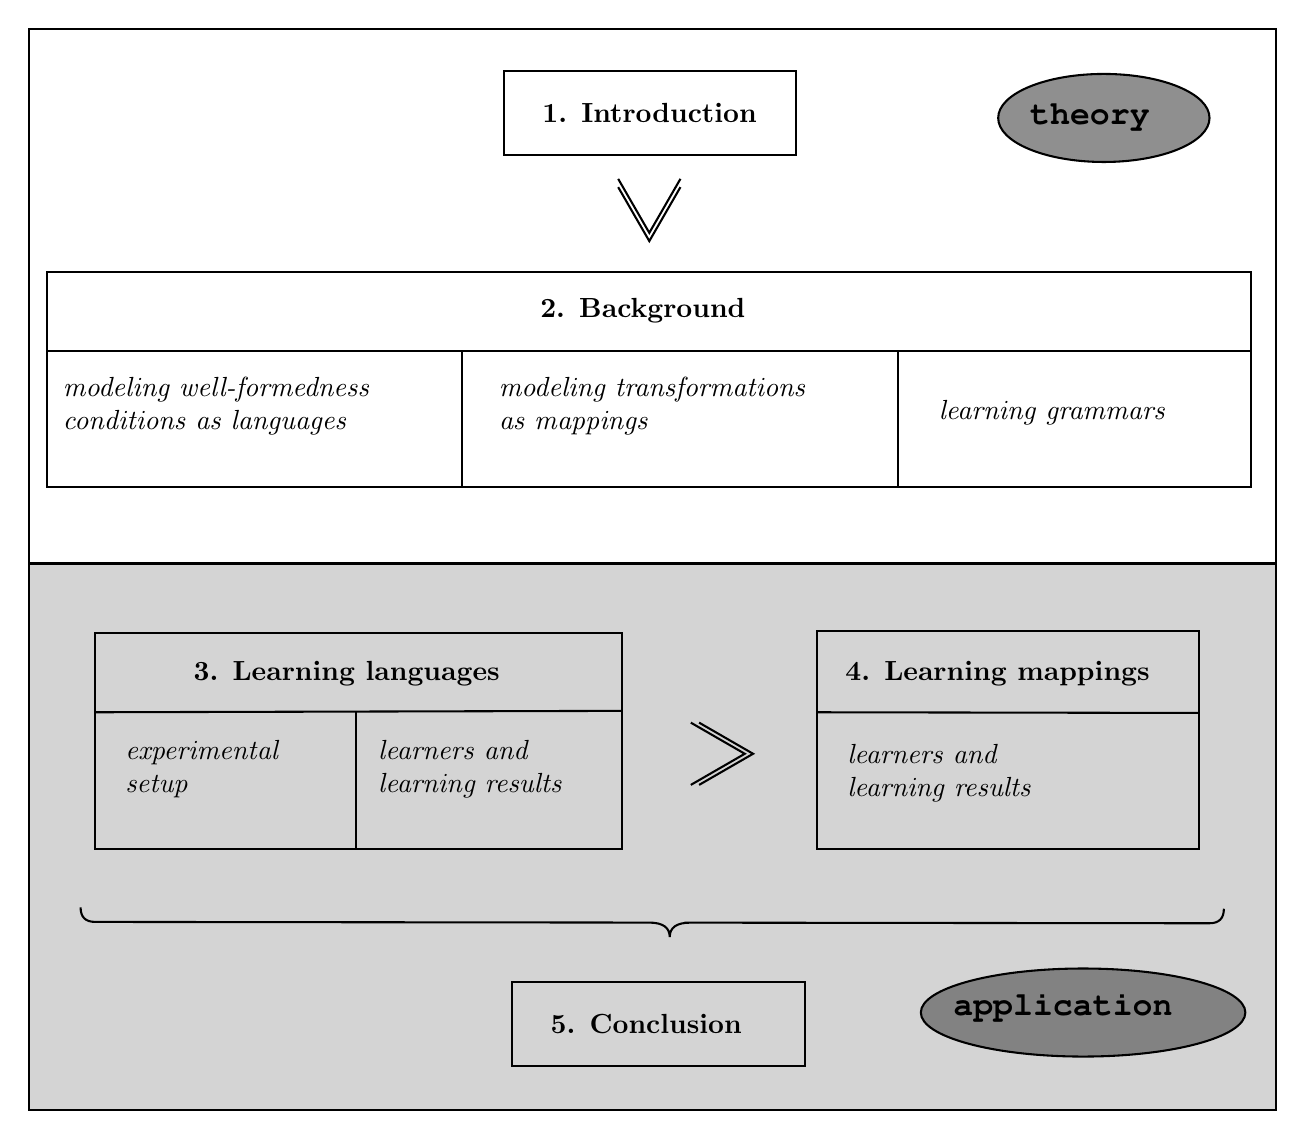
\begin{tikzpicture}[x=0.75pt,y=0.75pt,yscale=-1,xscale=1]
%uncomment if require: \path (0,538); %set diagram left start at 0, and has height of 538

%Shape: Rectangle [id:dp8221412876102787] 
\draw   (250,31) -- (390.83,31) -- (390.83,71.33) -- (250,71.33) -- cycle ;
%Shape: Rectangle [id:dp5026563864255413] 
\draw   (29.83,128) -- (609.83,128) -- (609.83,231.33) -- (29.83,231.33) -- cycle ;
%Straight Lines [id:da7513846337736221] 
\draw    (29.83,166) -- (609.83,166) ;
%Shape: Rectangle [id:dp8727441659717616] 
\draw   (52.83,302) -- (306.83,302) -- (306.83,406) -- (52.83,406) -- cycle ;
%Straight Lines [id:da08433324969296474] 
\draw    (52.83,340) -- (306.83,339.33) ;
%Shape: Rectangle [id:dp7150794601993389] 
\draw   (400.83,301) -- (584.83,301) -- (584.83,405.67) -- (400.83,405.67) -- cycle ;
%Straight Lines [id:da1691060851390651] 
\draw    (400.83,340) -- (584.83,340.33) ;
%Straight Lines [id:da8740251300311048] 
\draw    (229.83,166) -- (229.83,232) ;
%Straight Lines [id:da7832612810103501] 
\draw    (439.83,166) -- (439.83,232) ;
%Straight Lines [id:da3202514288331062] 
\draw    (178.83,340) -- (178.83,406) ;
%Shape: Rectangle [id:dp5815929836430904] 
\draw   (254,470) -- (394.83,470) -- (394.83,510.33) -- (254,510.33) -- cycle ;
%Shape: Rectangle [id:dp21095701304766612] 
\draw   (21,10.67) -- (621.83,10.67) -- (621.83,531.67) -- (21,531.67) -- cycle ;
\draw   (335,83) -- (320,109) -- (305,83)(335,87) -- (320,113) -- (305,87) ;
\draw   (340,345) -- (366,360) -- (340,375)(344,345) -- (370,360) -- (344,375) ;
%Shape: Brace [id:dp7711459734646808] 
\draw   (46,434) .. controls (45.99,438.67) and (48.32,441) .. (52.99,441.01) -- (319.84,441.33) .. controls (326.51,441.34) and (329.84,443.68) .. (329.84,448.35) .. controls (329.84,443.68) and (333.17,441.35) .. (339.84,441.36)(336.84,441.36) -- (589.82,441.66) .. controls (594.49,441.67) and (596.82,439.34) .. (596.83,434.67) ;
%Shape: Rectangle [id:dp23976569225238542] 
\draw  [fill={rgb, 255:red, 0; green, 0; blue, 0 }  ,fill opacity=0.17 ] (21,268.33) -- (621.83,268.33) -- (621.83,531.67) -- (21,531.67) -- cycle ;

% Text Node
\draw (267,45) node [anchor=north west][inner sep=0.75pt]   [align=left] {\textbf{1. Introduction}};
% Text Node
\draw (266,139) node [anchor=north west][inner sep=0.75pt]   [align=left] {\textbf{2. Background}};
% Text Node
\draw (36,177) node [anchor=north west][inner sep=0.75pt]   [align=left] {\textit{modeling well-formedness}\\\textit{conditions as languages}};
% Text Node
\draw (246,177) node [anchor=north west][inner sep=0.75pt]   [align=left] {\textit{modeling transformations}\\\textit{as mappings}};
% Text Node
\draw (458,188) node [anchor=north west][inner sep=0.75pt]   [align=left] {\textit{learning grammars}};
% Text Node
\draw (98.98,314) node [anchor=north west][inner sep=0.75pt]   [align=left] {\textbf{3. Learning languages}};
% Text Node
\draw (66.07,352) node [anchor=north west][inner sep=0.75pt]   [align=left] {\textit{experimental}\\\textit{setup}};
% Text Node
\draw (187.9,352) node [anchor=north west][inner sep=0.75pt]   [align=left] {\textit{learners and}\\\textit{learning results}};
% Text Node
\draw (412.98,314) node [anchor=north west][inner sep=0.75pt]   [align=left] {\textbf{4. Learning mappings}};
% Text Node
\draw (413.9,354) node [anchor=north west][inner sep=0.75pt]   [align=left] {\textit{learners and}\\\textit{learning results}};
% Text Node
\draw (271,484) node [anchor=north west][inner sep=0.75pt]   [align=left] {\textbf{5. Conclusion}};
% Text Node
\draw  [fill={rgb, 255:red, 0; green, 0; blue, 0 }  ,fill opacity=0.44 ]  (539, 53.67) circle [x radius= 50.91, y radius= 21.21]   ;
\draw (502,45) node [anchor=north west][inner sep=0.75pt]  [font=\large,color={rgb, 255:red, 0; green, 0; blue, 0 }  ,opacity=1 ] [align=left] {{\large {\fontfamily{pcr}\selectfont \textbf{theory}}}};
% Text Node
\draw  [fill={rgb, 255:red, 0; green, 0; blue, 0 }  ,fill opacity=0.39 ]  (529, 484.67) circle [x radius= 78.18, y radius= 21.21]   ;
\draw (465,474) node [anchor=north west][inner sep=0.75pt]  [font=\large,color={rgb, 255:red, 0; green, 0; blue, 0 }  ,opacity=1 ] [align=left] {\textbf{{\large {\fontfamily{pcr}\selectfont application}}}};

\end{tikzpicture}
}
\caption{Flow of chapters of this dissertation: Introduction, Background, Learning languages, Learning mappings, and Conclusion.}
\label{chaptersstructure}
\end{figure}




%\setcounter{chapter}{1}
\chapter{Background}
Linguistic rules capture two types of generalizations: \textbf{well-formedness conditions}, i.e.\ the requirements for a word to be well-formed, and \textbf{transformations}, i.e.\ the rules of re-computing the given underlying representation into the corresponding surface form.
Former restrict the word's form itself, such as ``two vowels should never be adjacent to each other'', while latter describe the change, such as ``insert {[}j{]} in-between two adjacent vowels''.
For example, transformations map the Russian word that is orthographically represented as \emph{dlinnosheee} `long-necked' into its pronunciation \emph{dlinnosh[ejeje]}, and the well-formedness conditions ensure that the pronunciation \emph{dlinnosh[eee]} is not allowed since it contains two vowels adjacent to each other.


\emph{Grammars} describe how to build well-formed words from the elements of the \emph{alphabet}.
A \emph{language} of the grammar is a potentially infinite collection of all well-formed strings of that grammar.
Thus in a formal sense, it simply refers to a collection of words, or \emph{strings}.
Transformations are functions from the \emph{input language}, i.e.\ a collection of ``underlying representations'', onto the \emph{output language}, or a collection of ``surface forms''.


In this chapter, I discuss \emph{subregular grammars} and \emph{subsequential functions} as they seem to be a good fit for natural language dependencies \citep[i.a.]{Heinz11part1,HeinzRawal11,GainorLai12,Heinz-Lai-2013-VHS,AksenovaEtAl16,Graf17CLSpres,ChandleeHeinz2018}.
In the two following chapters, I show the results of the \textbf{automatic extraction} of subregular grammars and subsequential functions given the learning framework defined in Section \ref{learningframework}.


\section{Modeling well-formedness conditions}

To model well-formedness conditions means to find a way to discriminate between well-formed and ill-formed words of a language.
In other words, it implies finding a \emph{grammar} that only builds well-formed strings, and that can recognize which strings are ill-formed.
For example, given the alphabet of vowels and consonants, a grammar can prohibit vowel hiatus by penalizing adjacent vowels.

Subregular grammars provide an interpretable and succinct way to encode such rules.
Interestingly, the subregular nature of linguistic generalizations allows us to explain the absence of some theoretically possible yet typologically unattested patterns \citep{GainorLai12}.
Also, this approach gives insights into human cognition since there is evidence that only some subregular language classes are learnable \citep{Lai15}.

\subsection{Regular nature of natural language patterns}

Consider a pattern of Russian compounding, where a morpheme \emph{-o-}%
\footnote{This marker is also sometimes realized as \emph{-e-}.}
 is located in-between compounding stems.
For example, the stems \emph{vod(-a)}%
\footnote{\emph{-a} is a suffix marking nominative case, singular form for some nominal classes.}
 `water' and \emph{voz} `carrier' can be combined to obtain a complex word \emph{vod-o-voz} `water carrier'.
If the compound is composed of multiple stems, the marker is added in-between every one of them: \emph{vod-o-voz-o-voz} `carrier of water carriers'.

This pattern can be viewed as a language of well-formed sequences of stems and compounding affixes.
Strings such as \emph{stem}, \emph{stem-o-stem}, \emph{stem-o-stem-o-stem} belong to the target language, but \emph{stem-stem} and \emph{stem-o} do not.
This can be rephrased a rule ``a well-formed form cannot start or end with a compounding marker, and within a word, two markers or two stems should not be adjacent to each other''.
Generalizations like this can be conveniently expressed as \textbf{finite state automata}.

A \textbf{finite state automaton} (FSA) is a type of an abstract machine that is defined by a finite list of states and the transitions between those states \citep{Lawson2003}.
In the case of string-based automata, these transitions are annotated with characters.
An automaton reads a string of characters (the \emph{input string}), and every new character changes the current state.
Some of the states are \emph{initial}, meaning that the first character of the input string can be read from those states.
\emph{Final}, or \emph{accepting} states are the ones that indicate that the string is accepted.
The input string is accepted by an automaton when the first character of that string can be read from the initial state, and this string is a path from the initial state to the final one.

Consider the automaton in Figure \ref{fig:ruscompounding}.
The numbered circles represent states, and the arrows are the transitions between those states.
States are usually referred to as $q$, therefore the states of that machine are $q_0$, $q_1$ and $q_2$. 
The initial state is represented with an incoming ``start'' arc.
The state $q_1$ is marked with a double circle, meaning that it is final.


\begin{figure}[h!]
\centering
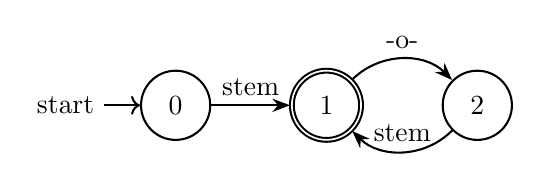
\begin{tikzpicture}
    \node (0) [state, accepting] {$1$};
    \node (1) [state, right=of 0] {$2$};
    \node (2) [state, left=of 0, initial] {$0$};
    \path [-{Stealth[]}]
      (0) edge[bend left = 45] node [above] {-o-} (1)
      (1)  edge[bend left = 45] node [above] {stem} (0)
      (2) edge node [above] {stem} (0)
      ;
  \end{tikzpicture}
\caption{FSA for Russian compounding.}
\label{fig:ruscompounding}
\end{figure}


A language of an FSA is a potentially infinite set of strings, every member of which can be recognized by that automaton.
For example, in Figure \ref{fig:ruscompounding}, the only possible transition from the initial state $q_0$ reads a stem and moves the machine to $q_1$.
The state $q_1$ is the accepting state, and any string that brings the automaton to the accepting state is well-formed with respect to the rules encoded in the automaton.
A single stem is therefore considered well-formed.
A compounding marker \emph{-o-} moves the machine from the state $q_1$ to $q_2$.
But $q_2$ is not final, so strings cannot be accepted if they end up in that state: the compounding marker cannot be the final element of the word.
The machine then necessarily returns to the state $q_1$, therefore accepting \emph{stem-o-stem}.
If more markers and stems follow, it takes the loop $q_1\rightarrow q_2\rightarrow q_1$ again.
The complexity of the language recognized by an FSA is not more than \emph{regular}.


\emph{Formal languages} are potentially infinite collections of strings produced according to the rules of some \emph{grammar}.
Different language classes can be recognized by different automata.
These automata can also be referred to as \emph{abstract machines}, a more general name for theoretically possible computers encoding the rules of those languages.
These machines, and therefore languages corresponding to them, can be ordered with respect to the complexity of the dependencies that they encode.
The first version of such a hierarchy was introduced in \cite{Chomsky1956} and is therefore known as \emph{the Chomsky hierarchy}.
Nowadays, we usually use an extended version of the hierarchy that includes \emph{mildly context-sensitive} and \emph{finite} language classes \citep{JagerRogers12}, see Figure \ref{fig:chomhier}.



%\begin{figure}[h!]
%\begin{center}
%\begin{tikzpicture}          
%	\draw (0,-0.65) ellipse (16em and 6em);    
%        \draw (0,-0.98) ellipse (14em and 5em);            
%        \draw (0,-1.3) ellipse (12em and 4em);            
%        \draw (0,-1.65) ellipse (10em and 3em);            
%        \draw (0,-1.97) ellipse (8em and 2em);            
%        \draw (0,-2.3) ellipse (6em and 1em);
%        %
%        \node at (0em,3em) {\textit{recursively enumerable}};
%        \node at (0em,1.1em) {\textit{context-sensitive}};
%        \node at (0em,-1em) {\textit{mildly context-sensitive}};
%        \node at (0em,-2.9em) {\textit{context-free}};
%        \node at (0em,-4.8em) {\textit{regular}};
%        \node at (0em,-6.8em) {\textit{finite}};
%\end{tikzpicture}
%\caption{The extended Chomsky hierarchy from \citep{JagerRogers12}.}
%\label{fig:chomhier}
%\end{center}
%\end{figure}



\begin{figure}[h!]
\begin{center}
\small
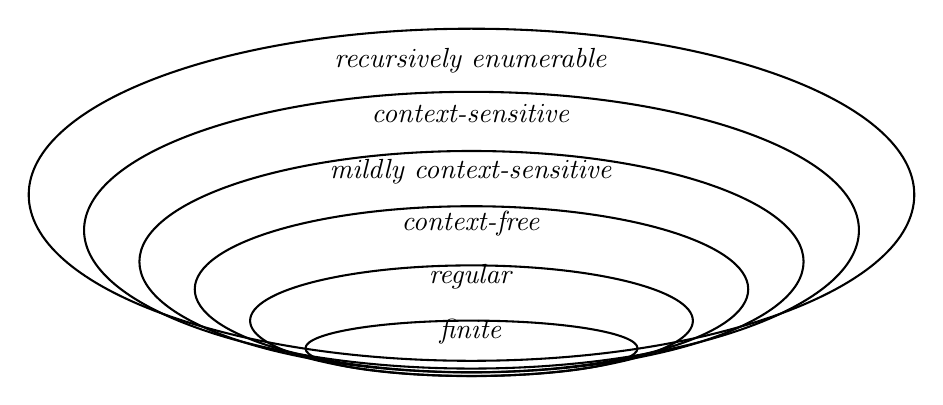
\begin{tikzpicture}          
	\draw (0,-0.65) ellipse (16em and 6em);    
        \draw (0,-1.1) ellipse (14em and 5em);            
        \draw (0,-1.5) ellipse (12em and 4em);            
        \draw (0,-1.85) ellipse (10em and 3em);            
        \draw (0,-2.25) ellipse (8em and 2em);            
        \draw (0,-2.6) ellipse (6em and 1em);
        %
        \node at (0em,3em) {\textit{recursively enumerable}};
        \node at (0em,1.1em) {\textit{context-sensitive}};
        \node at (0em,-1em) {\textit{mildly context-sensitive}};
        \node at (0em,-2.9em) {\textit{context-free}};
        \node at (0em,-4.8em) {\textit{regular}};
        \node at (0em,-6.8em) {\textit{finite}};
\end{tikzpicture}
\caption{The extended Chomsky hierarchy from \citep{JagerRogers12}.}
\label{fig:chomhier}
\end{center}
\end{figure}


This hierarchy represents nested classes of formal languages aligned with respect to their expressive complexity.
On the very top of the hierarchy, there are \textbf{recursively enumerable} languages.
Those are the languages that can be physically computed, i.e.\ realized by a computer in the universe\footnote{The current definition is based on the physical Church-Turing thesis \citep{Church1936,Turing1937a,Turing1937b}.} \citep{Chomsky1956}.
For example, a language $a^{n}$, where $n$ is a prime number, is recursively enumerable.
Below, there are \textbf{context-sensitive} languages that recognize non-linear%
\footnote{The non-linearity refers to the growth of the number of $a$: every following number is \emph{much} larger than the previous.}
 patterns such as $a^{2n}$, where $n$ is greater than $0$.
There are subclasses of context-sensitive languages which are a better fit for natural language syntax, such as \textbf{mildly context-sensitive} languages.
They are a good fit for syntactic dependencies as they handle cross-serial dependencies such as some cases of copying \citep{Joshi1985,Shieber1985,Kallmeyer2010}.
The machine corresponding to \textbf{context-free} languages uses a stack of a potentially infinite size: in such a way, it recognizes patterns such as $a^{n}b^{n}$, \emph{``have as many $a$ as $b$''} \citep{HopcroftEtAl2006}.
\textbf{Regular} languages are limited to the dependencies that can be recognized by an FSA \citep{HopcroftEtAl2006}.
It is commonly assumed that morphology and phonology are regular \citep{Johnson1972,KaplanKay94,BeesleyKartunnen03,RoarkSproat2007}, and I will come back to this topic in the following paragraphs.
Finally, at the very bottom of the hierarchy, one can see a class of \textbf{finite} languages that refer to a finite number of strings.
Classes that are more complex than mildly context-sensitive dependencies are rarely discussed in connection with natural languages: they are too powerful.

Finite-state models correspond to regular languages, and were introduced in $1940$s by \citeauthor{McCullochPitts1943}.
\cite{Chomsky1956}, however, theorized that this type of modeling does not seem to be suitable for natural languages, although in the following years his arguments were shown to be wrong.
Despite that, there was a significant number of applications of finite-state machines to language-related tasks, such as text search \citep{Thompson1968}, machine translation \citep{OncinaEtAl1994,KnightAlOnaizan1998,BangaloreRiccardi2002}, speech recognition \citep{Caseiro2003,MohriPereiraRiley2002,MohriPereiraRiley2008}, semantic parsing \citep{JonesJohnsonGoldwater2011,JonesJohnsonGoldwater2012}, and others.
The restrictiveness of finite-state models is frequently used to balance the robustness of neural networks.
For example, a neural FST-based pronunciation learning model was designed by \cite{Bruguier2017PronunciationLW}.
Additionally, \cite{RoarkEtAl2019} use a neural network guided by a regular grammar to assign pronunciations to words.
At the same time, linguists and computer scientists started to employ regular languages and finite-state models as a tool to research the complexities of patterns in human languages, see \cite{Hulden2014} discussing the main milestones.



The regular nature of phonology was examined several decades ago by \citep{Johnson1972,Kaplan1981PhonologicalRA,KaplanKay94}.
Importantly, \cite{KaplanKay94} show that all SPE-style transformational rules \citep{ChomskyHalle1968}, can be represented as finite-state machines.
Since all attested phonological patterns can be modeled as SPE-style rules, and since SPE-style rules are regular, the complexity of regular languages is a good upper bound for phonological dependencies.
In the same paper, they also presented a set of modeling tools and used them to capture patterns such as nasal assimilation and epenthesis.


\cite{Koskenniemi1983}, and later \cite{BeesleyKartunnen03} show that finite-state machinery is sufficient for encoding morphological dependencies as well.
Even the non-concatenative morphology can be modeled in such a way \citep{Kay1987,Beesley1996,Kiraz1996}.
For more examples of applications of finite-state methods in linguistics, see \citep{GildeaJurafsky1996,RocheSchabes1997,Hetherington2001,JurafskyMartin2009}.
Although regular languages are a good fit for linguistic patterns, research shows that the full power of regular languages is not necessary, and \emph{subregular} languages that are discussed further provide a tighter fit for phonology and morphology.


\subsection{Subregular languages and their linguistic importance}
\label{subgsgf}

The class of regular languages can be subdivided into a nested hierarchy of \emph{subregular} classes -- \emph{subregular hierarchy}.
``Parent'' classes are more powerful than their ``children'' classes, and therefore properly include them.
The ``sibling'' relation implies that the classes are not known to subsume each other.
Some of the classes of the subregular hierarchy are presented below in Figure \ref{subreghier}.

\begin{figure}[h!]
\begin{center}
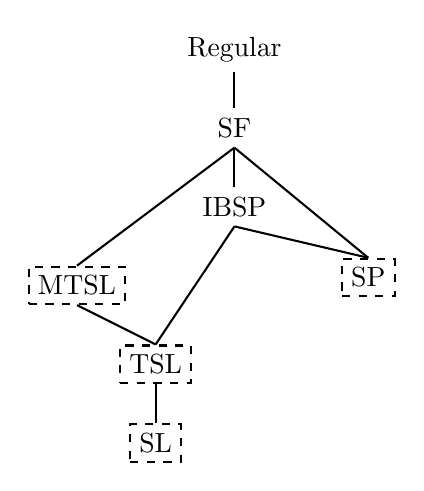
\begin{tikzpicture}[
    highlight/.style = { draw, rectangle, dashed }
    ]
\node (R) at (0,9.5) {Regular};
\node (SF) at (0,8.5) {SF};
\node (IBSP) at (0,7.5) {IBSP};
\node[highlight] (MTSL) at (-2,6.5) {MTSL};
\node[highlight] (TSL) at (-1,5.5) {TSL};
\node[highlight] (SP) at (1.7,6.6) {SP};
\node[highlight] (SL) at (-1,4.5) {SL};
%
\foreach \Source/\Target in {%
        R.south/SF.north,
        SF.south/MTSL.north,
        SF.south/IBSP.north,
        SF.south/SP.north,
        MTSL.south/TSL.north,
        IBSP.south/TSL.north,
        IBSP.south/SP.north,
        TSL.south/SL.north%
    }
\draw (\Source) to (\Target);
\end{tikzpicture}
\caption{Some of the classes of the subregular hierarchy; the subregular classes discussed further in this chapter and in Chapter 3 are boxed.}
\label{subreghier}
\end{center}
\end{figure}

Figure \ref{subreghier} shows some of the subregular classes, namely the ones that are crucially important for modeling linguistic dependencies, and therefore extensively used in this dissertation.
Namely, those are strictly local (SL), strictly piecewise (SP), tier-based strictly local (TSL) and multi-tier strictly local (MTSL) languages.
The crucial difference between these languages is in the types of dependencies they can capture, see Table \ref{subregclasses}.
The combined functionality of those classes covers local dependencies and long-distance dependencies with or without a blocker.


\begin{table}[h!]
\begin{center}
\begin{tabular}{|l|l|}
\hline
\textbf{Language}      & \textbf{Dependencies it can handle}                       \\ \hline
\textit{\textbf{SL}}   & only local dependencies                                   \\ \hline
\textit{\textbf{SP}}   & only multiple long-distance dependencies without blocking \\ \hline
\textit{\textbf{TSL}}  & long-distance dependencies with blocking                  \\ \hline
\textit{\textbf{MTSL}} & multiple long-distance dependencies with blocking         \\ \hline
\end{tabular}
\caption{Types of dependencies captured by some of the subregular classes.}
\label{subregclasses}
\end{center}
\end{table}



Subregular languages are encoded by \emph{subregular grammars}.
These subregular grammars operate by blocking some types of substrings or subsequences in well-formed strings of their languages.
A \textbf{substring} is a consecutive part of the string.
For example, \emph{ab}, \emph{aba}, and \emph{abacd} are substrings of the string \emph{abacd}, whereas \emph{aa} and \emph{bcd} are not, because these symbols are not adjacent in the string \emph{abacd}.
\textbf{Subsequences} can be seen as a non-consecutive counterpart of substrings.
A string $u$ is a subsequence of $w$ if all elements of $u$ can be found in $w$, and the order of those elements is preserved.
Continuing the previous example, both \emph{aa} and \emph{bcd} are indeed subsequences of \emph{abacd}.
Importantly, the elements of substrings and subsequences cannot violate the order in which the elements appeared in the original string: \emph{ca} is neither a substring nor a subsequence of the string \emph{abacd}.
Subregular grammars are always defined for some particular locality, so a $2$-local grammar operates with substrings or subsequences of the length $2$.
Formally, substrings and subsequences are defined in Definitions 2.1.1 and 2.1.4, and in \citep[a.o.]{ElzingaEtAl2008,Rogers-HeinzEtAl-2010-LPTSS,Fu2011}.

While \emph{positive grammars} list all allowed substructures of their languages, the \emph{negative} ones list the substructures that must not be encountered in well-formed strings of their languages. Moreover, these grammars are equivalent, i.e.\ for every negative grammar, it is possible to construct a positive grammar that generates the same language, and vice versa.

The above mentioned subregular grammars are negative, so they prohibit certain substructures in well-formed strings of their languages.
\textbf{Strictly local} (SL) grammars filter strings that violate some local dependency in the string, i.e.\ contain ill-formed \emph{substrings} \citep{Heinz-2010-SEL}.
For example, a language \emph{ab, abab, ababab, etc.} contains any possible string of $a$ and $b$ that does not contain the substrings $aa$ and $bb$.
\textbf{Tier-based strictly local} (TSL) grammars project a potentially smaller string from the input string by using a tier alphabet.
These grammars evaluate the relatively local dependencies among the elements of the \emph{tier alphabet}, whereas all other symbols are ``transparent'' for the grammar \citep{HeinzRawal11}.
For example, if the tier contains $a$ and $b$ and the string is $bccacbc$, the \emph{tier image} of that string is $bab$.
TSL constraints such as $ba$ or $ab$ would rule out that string.
\textbf{Multi-tier strictly local} (MTSL) grammars can have more than just a single tier, and, therefore, multiple tier images are evaluated with respect to multiple local grammars \citep{DeSantoGraf19FG}.
\textbf{Strictly piecewise} (SP) grammars restrict certain \emph{subsequences} in well-formed strings of their languages \citep{Rogers-HeinzEtAl-2010-LPTSS,Heinz10ldp}.
For example, if a subsequence $xx$ is prohibited, a string $xaaax$ is ruled out.
In such a way, SL, SP, TSL and MTSL grammars model a wide range of local and long-distant processes \citep{Heinz11part1,HeinzRawal11,Heinz-Lai-2013-VHS,AksenovaEtAl16,ChandleeHeinz2018}.
There are other subregular classes not listed here such as star free, interval-based strictly piecewise, input-output tier-based strictly local, piecewise testable, etc., but they are out of scope of this dissertation \citep{Lawson2003,Graf18NELS}.
Additionally, I will only discuss grammars working with strings, but this approach is currently extended to other representations as well \citep{chandlee-etal-2019-learning,chandlee-jardine-2019-autosegmental}.

The \emph{strong subregular hypothesis} suggests that a regular bound is too powerful for natural language phonology and phonotactics and that subregular languages are a better fit \citep{Heinz10ldp}.
%Four subregular classes -- SL, SP, TSL, and MTSL -- fit most of the natural language dependencies.
%An SL grammar puts restrictions on $n$-local \emph{substrings}, therefore it captures only local dependencies.
%An SP grammar cannot express local processes because it prohibits \emph{subsequences}, i.e.\ not necessarily adjacent sequences of elements.
%As a result, it captures long-distant dependencies such as some harmonies and UTP, but cannot model blocking effect.
%A TSL grammar captures blocking by projecting all elements participating in the harmony on the tier, therefore, creating the locality relation among them.
%However, a TSL grammar cannot capture several long-distance agreements if they target different sets of participants.
%An MTSL grammar projects several tiers, therefore every observed agreement is captured by its own tier.
In line with phonotactics, \cite{AksenovaEtAl16} shows that subregular languages are a good fit for morphotactic dependencies.
The well-formedness conditions imposed on languages of generalized and monomorphemic quantifiers are also subregular.
There are likewise applications of subregular grammars to syntax  \citep{Graf17Rutgerstalk,DeSantoGrafDrury2017,VuEtAl19SCiL}.

In the rest of the chapter, I focus on SL, SP, TSL and MTSL languages and grammars, and provide linguistically-motivated examples of those.
Additionally, I define these classes mathematically and describe the corresponding classes of finite-state automata.
Later, in chapter 3, I will model those and some other dependencies, and show how their subregular grammars can be learned from real data.
Table \ref{fig:subrepattenslfg} summarizes patterns that are discussed further and subregular classes to which they belong.


\begin{table}[h!]
\centering
\begin{tabular}{|>{\centering\arraybackslash}m{0.2\textwidth}|>{\centering\arraybackslash}m{0.2\textwidth}|>{\centering\arraybackslash}m{0.2\textwidth}|>{\centering\arraybackslash}m{0.2\textwidth}|}
\hline
 \centering \textbf{SL} & \centering \textbf{SP}                   & \centering \textbf{TSL} & \textbf{MTSL} \\ \hline
\multicolumn{4}{|c|}{\textit{word-final devoicing and obstruent voicing assimilation}}                                       \\ \hline
                      {\Large\faCheck}        &    \cellcolor{gray!50}\faTimes                           &                             {\Large\faCheck} &          {\Large\faCheck}                     \\ \hline
\multicolumn{4}{|c|}{\textit{unbounded tone plateauing}}                                                                     \\ \hline 
          \cellcolor{gray!50}\faTimes                    &                              {\Large\faCheck} &               \cellcolor{gray!50}\faTimes               &                              \cellcolor{gray!50}\faTimes \\ \hline
\multicolumn{4}{|c|}{\textit{sibilant harmony in voicing and anteriority, no blockers}}       \\ \hline
                  \cellcolor{gray!50}\faTimes            &                              {\Large\faCheck} &                   {\Large\faCheck}           &{\Large\faCheck}                               \\ \hline
\multicolumn{4}{|c|}{\textit{vowel harmony in ATR, nasalized vowels are blockers}}             \\ \hline
                  \cellcolor{gray!50}\faTimes            &                              \cellcolor{gray!50}\faTimes &            {\Large\faCheck}                  &   {\Large\faCheck}                            \\ \hline
\multicolumn{4}{|c|}{\textit{vowel harmony in ATR and rounding, some vowels are blockers for rounding}}             \\ \hline
                  \cellcolor{gray!50}\faTimes            &                              \cellcolor{gray!50}\faTimes &            {\Large\faCheck}                  &   {\Large\faCheck}                            \\ \hline
\multicolumn{4}{|c|}{\textit{sibilant harmony in voicing and anteriority, voiceless obstruents are blockers for voicing}} \\ \hline
                      \cellcolor{gray!50}\faTimes        &                              \cellcolor{gray!50}\faTimes &              \cellcolor{gray!50}\faTimes                &  {\Large\faCheck}  \\ \hline
\end{tabular}
\caption{Subregular patterns attested in natural languages and discussed in sections 2.1.3-6.}
\label{fig:subrepattenslfg}
\end{table}



\subsection{Local restrictions as SL languages}
\label{russianwfdpatternn}

The subregular class of strictly local (SL) languages captures local dependencies, and many restrictions in phonology have a purely local nature \citep{RogersPullum2011}.
Indeed, most of the patterns of phonological assimilation affect adjacent segments.
In what follows, I exemplify SL languages using several purely local processes, and then formally introduce them using the notion of $k$-factor and the property of suffix substitution closure \citep{RogersEtAl13}.

\subsubsection{Intuitive definition}

In what follows, the SL languages are demonstrated through two local processes happening in Russian: one of them prohibits voiced obstruents in the word-final position, and another one enforces adjacent obstruents to agree in voicing.
Additionally, I show the interaction between these two patterns.

\paragraph{Russian obstruent assimilation and word-final devoicing}
The examples (1-2) below show that the consonant of the preposition \emph{iz} `from' agrees in voicing with the obstruent of the following word.%
\footnote{I do not discuss exceptions to this rule, such as the well-formedness of the cluster [sv].}

\medskip
\begin{tabular}{lll}
(1) & i[z B]erlina & `from Berlin' \\
(2) & i[s P]ragi & `from Prague'
\end{tabular}
\medskip

Additionally, in Russian, as well as in other languages such as German, there is a process of word-final devoicing that prohibits the appearance of a voiced obstruent in a word-final position \citep{Wiebke1995,Padgett2002ms}.
For example, \emph{lug} `field' is realized as \emph{lu[k]}.
In this case, the same cluster of obstruents might appear voiceless word-finally, and voiced in other positions of the word, see the pairs of examples in (3-4) and (5-6).

\medskip
\begin{tabular}{lllclll}
(3) & mo[sk] & `brain' & $\sim$ & (4) & mo[zg]i & `brains' \\
(5) & dro[st] & `thrush' & $\sim$ & (6) & dro[zd]y & `thrushes'
\end{tabular}
\medskip

These two generalizations can be captured in a \emph{strictly local} way, namely, by prohibiting illicit substrings.
Assume that the inventory of obstruents is $\{z, s, b, p, g, k\}$, where $z$, $b$, and $g$ are voiced, and $s$, $p$ and $k$ are voiceless.
It is never possible to see two (or more) disagreeing obstruents adjacent to each other, i.e.\ the target SL grammar needs to prohibit $zs$, $zp$, $zk$, $sz$, $sb$, $sg$, etc.


To target voiced obstruents at the end of the word, the grammar needs to be able to differentiate between the word-final and other positions.
For this reason, strings are usually annotated with the markers \bow\ and \eow\ denoting the beginning and the end of the string \citep{RogersPullum2011}.
Then, the SL grammar capturing word-final devoicing needs to rule out $z\eow$,  $g\eow$, and $b\eow$.

\begin{figure}[h!]
\begin{center}
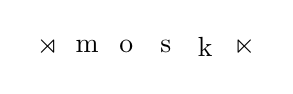
\begin{tikzpicture}
\node (1) at (0,0) {$\rtimes$};
\node (2) at (0.5,0) {m};
\node (3) at (1,0) {o};
\node (4) at (1.5,0) {s};
\node (5) at (2,0) {k};
\node (6) at (2.5,0) {$\ltimes$};
\end{tikzpicture}
\hspace{2em}
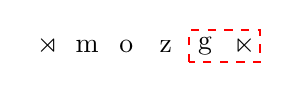
\begin{tikzpicture}
\node (1) at (0,0) {$\rtimes$};
\node (2) at (0.5,0) {m};
\node (3) at (1,0) {o};
\node (4) at (1.5,0) {z};
\node (5) at (2,0) {g};
\node (6) at (2.5,0) {$\ltimes$};
\draw [dashed, red] (1.8, -0.2) -- (1.8, 0.2) -- (2.7, 0.2) -- (2.7, -0.2) -- (1.8, -0.2);
\end{tikzpicture}
\vspace{1em}

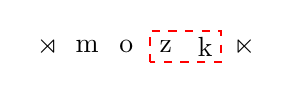
\begin{tikzpicture}
\node (1) at (0,0) {$\rtimes$};
\node (2) at (0.5,0) {m};
\node (3) at (1,0) {o};
\node (4) at (1.5,0) {z};
\node (5) at (2,0) {k};
\node (6) at (2.5,0) {$\ltimes$};
\draw [dashed, red] (1.3, -0.2) -- (1.3, 0.2) -- (2.2, 0.2) -- (2.2, -0.2) -- (1.3, -0.2);
\end{tikzpicture}
\hspace{2em}
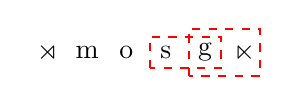
\begin{tikzpicture}
\node (1) at (0,0) {$\rtimes$};
\node (2) at (0.5,0) {m};
\node (3) at (1,0) {o};
\node (4) at (1.5,0) {s};
\node (5) at (2,0) {g};
\node (6) at (2.5,0) {$\ltimes$};
\draw [dashed, red] (1.3, -0.2) -- (1.3, 0.2) -- (2.2, 0.2) -- (2.2, -0.2) -- (1.3, -0.2);
\draw [dashed, red] (1.8, -0.3) -- (1.8, 0.3) -- (2.7, 0.3) -- (2.7, -0.3) -- (1.8, -0.3);
\end{tikzpicture}
\end{center}
\caption{Evaluation of strings \emph{mozg}, \emph{mozk}, \emph{mosg} and \emph{mosk} by an SL grammar capturing obstruent cluster assimilation and word-final devoicing.}
\label{mozgi}
\end{figure}

Figure \ref{mozgi} shows how the SL grammar outlined above evaluates the pronunciations \emph{mozg}, \emph{mozk}, \emph{mosg} and \emph{mosk}.
The string \emph{mozg} has its obstruents agree in voicing, but the final obstruent is voiced, and therefore ruled out by the restriction $g\eow$.
The final obstruent in \emph{mozk} is voiceless, but now the cluster disagrees and therefore ruled out by $zk$.
In \emph{mosg}, both violations are present.
Finally, the form \emph{mosk} contains no violations, and indeed, this is the correct pronunciation of the corresponding Russian word.

The illicit substrings such as $g\eow$ and $zk$ are the \emph{restrictions} defined by the grammar.
A set of restrictions $R$ of a negative grammar lists all substrings that \emph{cannot} be found in well-formed strings of the language.
An \emph{alphabet} of the language, usually denoted as $\Sigma$, includes the list of symbols the language uses.
In this case, $\Sigma$ includes all Russian phonemes.
Finally, every grammar defines its \emph{locality}, namely, the size of the longest string prohibited by that grammar; it is usually referred to as $k$ \citep{McNaughtonPapert1971,RogersPullum2011}.
In the case of the SL grammar capturing Russian well-formedness conditions, all the prohibited strings are of length $2$ ($k=2$); such substrings are also called \emph{bigrams} or \emph{factors}.
The Russian SL grammar is then strictly $2$-local, or $2$-SL.
These three components -- the alphabet $\Sigma$, the set of restriction $R$, and the locality window $k$ -- define SL grammars, see Grammar \ref{slwfdocass55}.

{
\renewcommand{\tablename}{Grammar}
\begin{table}[h!]
\begin{center}
\begin{tabular}{rl}
\textit{SL grammar}  & Russian obstruent voicing assimilation and word-final devoicing \\
\textit{$\Sigma$ =}      &  \{a, b, v, g, d $\dots$ z, s, p, k $\dots$ \textepsilon, $^j$u, $^j$a\}   \\
\textit{$R$ =} & $\langle$zs, zp, zk, sz, sb, sg $\dots$ z\eow,  g\eow, b\eow, d\eow $\rangle$  \\
\textit{$k$ =}      & $2$          
\end{tabular}
\caption{$2$-SL grammar for Russian obstruent voicing assimilation and word-final devoicing.}
\label{slwfdocass55}
\end{center}
\end{table}
}

SL grammars disallow the appearance of the banned clusters such as $gs$ or $zk$, however, they do not induce the change of the ill-formed segments.
The perspective of changing one form into another is examined in the Section 2.2 discussing modeling transformations.
SL models are useful in modeling the well-formedness conditions arising from word-final devoicing, intervocalic voicing, consonant cluster assimilation, and other local processes.
However, SL models cannot model long-distance dependencies.

\paragraph{Tuareg sibilant harmony}
Long-distance dependency affects segments that can be located far from each other.
For instance, in Tuareg (Berber), sibilants regressively agree in voicing and anteriority \citep{Hansson2010ber}.
In the examples below, a causative prefix agrees with the sibilant in the root (8-11) but is realized as \emph{s-} if no other sibilant is present (7).
This agreement is long-distant, and therefore it can happen across an arbitrary number of intervening elements.

\medskip
\begin{tabular}{lll}
(7) & s-\textschwa lm\textschwa d & `\textsc{caus}-learn' \\
(8) & s-\textschwa q:us\textschwa t & `\textsc{caus}-inherit' \\
(9) & z-\textschwa nt\textschwa z & `\textsc{caus}-extract' \\
(10) & \textesh-\textschwa m:\textschwa\textesh\textschwa n & `\textsc{caus}-be.overwhelmed' \\
(11) & \textyogh-\textschwa k:u\textyogh\textschwa t & `\textsc{caus}-saw'
\end{tabular}
\medskip

SL grammars capture only local generalizations, but, for example, in (9), there are $4$ elements separating the agreeing sibilants.
It would imply that the required locality of the SL grammar is at least $6$ to accommodate the two sibilants and everything in-between them.
However, this would not be enough for other cases since there is no upper bound on the number of the intervening segments in-between two agreeing sibilants.
As a result, the power of SL grammars is not enough to capture patterns such as Tuareg sibilant harmony.



\subsubsection{Formal definition}

SL grammars define languages by listing substrings that cannot appear in well-formed words of those languages.
These substrings are often referred to as $k$-factors, in order to be distinguished from the more NLP-oriented use of the term $n$-gram, that frequently implies the use of probabilistic models \citep{RogersPullum2011,RogersEtAl13}.
Further in this section, I follow \cite{DeSantoGraf19FG} in their algebraic definition of this class.

While $\Sigma$, as previously in this section, denotes the alphabet, $\Sigma^{k}$ is a $k$-long word that uses symbols of that alphabet.
$\Sigma^{*}$ generalizes $\Sigma^{k}$, it employs the \emph{Kleene star} \citep{Kleene1956} to define a word of any length.
A length of the string $w$ is denoted as $|w|$.

\begin{definition}[\textbf{$k$-factors}]
A string $u$ is a $k$-\emph{factor} of a string $w$ iff $\exists x, y \in \Sigma^*$ such that $w=xuy$ and $|u| = k$. 
The function $F_k$ maps words to the set of $k$-factors within them:
$$
F_k(w) = \{ u : u \textit{ is a $k$-factor of } w \textit{ if } |w| \geq k, 
\textit{ else } u = w\}
$$
\end{definition}

For example, the $2$-factors of the word $abc$ are $\{ab, bc\}$.
Strictly $k$-local grammars list the $k$-factors that cannot be used in the well-formed strings of their languages, i.e.\ they can be viewed as collections of illicit $k$-factors.

\begin{definition}[\textbf{SL languages and grammars}]
A language $L$ is \emph{strictly $k$-local} (SL$_k$) iff there exists a finite set $S \subseteq F_k (\rtimes^{k-1} \Sigma^* \ltimes^{k-1})$ such that
\[
L = \{ w \in \Sigma^*: F_k(\rtimes^{k-1} w \ltimes^{k-1}) \cap S = \emptyset \}.
\]
We call $S$ a strictly $k$-local grammar, and use $L(S)$  to indicate the language recognized by $S$.
A language $L$ is strictly local iff it is SL$_k$ for some $k \in \mathbb{N}$.
\end{definition}

Consider a language described by a regular expression $(ab)^{*}$.
Its language includes strings such as $\epsilon$, $ab$, $abab$, $ababab$, etc.
A negative $2$-SL grammar that describes this language is $S = \{\bow b, a\eow, aa, bb\}$.
Indeed, the well-formed strings of that language cannot start with $b$, end with $a$, and have two $a$ or two $b$ adjacent to each other.
Importantly, a language is strictly $k$-local if it satisfies $k$-local \emph{suffix substitution closure} \citep{RogersPullum2011}.

\begin{definition}[\textbf{Suffix substitution closure}]
\label{suffsubclosure}
For any $k \geq 1$, a language $L$ satisfies  $k$-local suffix substitution closure iff for all strings $u_1, v_1, u_2, v_2$, for any string $x$ of length $k - 1$ if both $u_1 \cdot x \cdot v_1 \in L$ and $u_2 \cdot x \cdot v_2 \in L$, then $u_1 \cdot x \cdot v_2 \in L$.
\end{definition}

For instance, a language $(ab)*$ is $2$-SL, and it satisfies the suffix substitution closure.
Both strings \emph{\textbf{a}b} and \emph{ab\textbf{a}bab} contain the $1$-local substring $a$, and it correctly predicts that the string \emph{ab\textbf{a}b} is also in the language.
However, a language $a^*ba^*$ is not SL.
It is not $2$-SL since the closure of the strings \emph{\textbf{a}ba} and  \emph{b\textbf{a}a} contains \emph{b\textbf{a}ba}, and it is not in the language.
It is not $3$-SL, because the closure of \emph{\textbf{aa}ba} and \emph{b\textbf{aa}a} contains the illicit form \emph{b\textbf{aa}ba}; and so on.
The language $a^*ba^*$ is not closed under the suffix substitution, and therefore it is not SL.

Apart from the algebraic perspective, strictly local languages can be characterized in automata-theoretic terms.
\cite{RogersPullum2011} describe SL languages as those that can be recognized by FSAs scanning a $k$-symbol window across the input string, and failing on strings that contain factors prohibited by the corresponding grammar.


\subsection{Long distance restrictions as SP languages}
\label{SPldrestrictions}


While SL grammars can only capture local dependencies, strictly piecewise (SP) grammars generalize exclusively long-distance patterns: %
%Previously, I showed that there is no upper bound on the amount of material in-between two agreeing sibilants, and therefore such generalization cannot be captured locally.
SL grammars prohibit sequences of adjacent segments within words, while SP grammars do not have the requirement of adjacency.
An SP restriction prohibits a certain \emph{order} of elements \citep{Rogers-HeinzEtAl-2010-LPTSS,Fu2011}. 
While an SL restriction $VV$ prohibits two vowels adjacent to each other thus avoiding hiatus, the same SP restriction means that nowhere in the string can there be a vowel followed by another vowel.
The language of such an SP grammar would only include words with no more than a single $V$.


\subsubsection{Intuitive definition}

In this section, I demonstrate how SP grammars can capture patterns of sibilant harmony and unbounded tone plateauing.
SP grammars encode restrictions on the order of elements, and thus cannot differentiate between disharmonic stems and grammatical words exhibiting a blocking effect.





\paragraph{Tuareg sibilant harmony}
Coming back to the pattern of Tuareg sibilant harmony exemplified before in (7-11), it can be modeled with an SP grammar by prohibiting subsequences of disagreeing sibilants.
The bigrams $sz$ and \textesh\textyogh~ are prohibited because their elements disagree in voicing, \textesh$s$ and $z$\textyogh~ disagree in anteriority, etc.
In total, this grammar contains $12$ restrictions $R$ that are listed in Grammar \ref{tuaregsibilanthupd}.

{
\renewcommand{\tablename}{Grammar}
\begin{table}[h!]
\begin{center}
\begin{tabular}{rl}
\textit{SP grammar}  & Tuareg sibilant harmony in voicing and anteriority \\
\textit{$\Sigma$ =}      &  \{s, \textyogh, z, \textesh, \textschwa, d, l, m, t $\dots$\}   \\
\textit{$R$ =} & $\langle$sz, s\textesh, s\textyogh, zs, \textesh s, \textyogh s, z\textesh, z\textyogh, \textesh s, z\textesh, z\textyogh, \textesh z, \textesh z, \textesh\textyogh, \textesh z$\rangle$  \\
\textit{$k$ =}      & $2$          
\end{tabular}
\caption{$2$-SP grammar for Tuareg sibilant harmony in voicing and anteriority.}
\label{tuaregsibilanthupd}
\end{center}
\end{table}
}

Such an SP grammar has an alphabet that includes all Tuareg phonemes, and its list of restrictions includes all pairs of sibilants disagreeing in voicing or anteriority.
The locality of such grammar is $2$.
Figure \ref{tuaregsthfg} shows that there are no violations in the word \emph{z\textschwa nt\textschwa z}: indeed, no substructure of that string is prohibited.
However, the word \emph{z\textschwa nt\textschwa \textyogh} is ruled out because the subsequence $z$\textyogh~ is ill-formed.


\begin{figure}[h!]
\begin{center}
\begin{tikzpicture}
\node (2) at (0.5,0.57) {z};
\node (3) at (1,0.57) {\textschwa};
\node (4) at (1.5,0.57) {n};
\node (5) at (2,0.57) {t};
\node (6) at (2.5,0.57) {\textschwa};
\node (7) at (3,0.57) {z};
\node (8) at (3,0) {\textcolor{white}{t}};
\end{tikzpicture}
\hspace{3em}
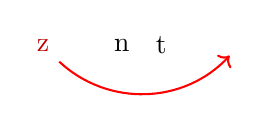
\begin{tikzpicture}
\node (2) at (0.5,0) {\textcolor{red!75!black}{z}};
\node (3) at (1,0) {\textschwa};
\node (4) at (1.5,0) {n};
\node (5) at (2,0) {t};
\node (6) at (2.5,0) {\textschwa};
\node (7) at (3,0) {\textcolor{red!75!black}{\textyogh}};
\path[->, red] (2) edge[bend right = 45] (7);
\end{tikzpicture}
\end{center}
\caption{Evaluation of strings \emph{z\textschwa nt\textschwa z} and \emph{z\textschwa nt\textschwa\textyogh} by an SP grammar capturing sibilant harmony in voicing and anteriority.}
\label{tuaregsthfg}
\end{figure}




\paragraph{Imdlawn Tashlhiyt sibilant harmony}

Now, consider a language closely related to Tuareg, namely, Imdlawn Tashlhiyt (Berber), in which affixal sibilants also regressively harmonize with the stem in voicing and anteriority \citep{Hansson2010ber,McMullin2016}.
The difference is that in Imdlawn Tashlhiyt, the spreading of the voicing feature can be blocked by any intervening voiceless obstruent.
At the same time, similarly to Tuareg, the anteriority harmony exhibits no blocking effect.
Consider the data from \citep{Elmedlaoui1995,Hansson2010} in (12-18), where the causative prefix \emph{s-} illustrates the harmonic pattern.

\medskip
\begin{tabular}{lll}
(12) & s:-uga & `\textsc{caus}-evacuate' \\
(13) & s-as:twa & `\textsc{caus}-settle' \\
(14) & \textesh-fia\textesh r & `\textsc{caus}-be.full.of.straw' \\
(15) & z-bruz:a & `\textsc{caus}-crumble' \\
(16) & \textyogh-m:\textyogh dawl & `\textsc{caus}-stumble' \\
(17) & s-m\textchi azaj & `\textsc{caus}-loathe.each.other' \\
(18) & \textesh-qu\textyogh:i & `\textsc{caus}-be.dislocated'
\end{tabular}
\bigskip

In (12), there are no sibilants in the root, so the prefix is realized as \emph{s-}.
Examples (13-16) show that as previously, the causative affix agrees with the stem sibilant in voicing and anteriority.
However, the voicing harmony can be blocked, and it is exemplified in (17) and (18).
In (17), the sibilants are both anterior, but \textchi~ is stopping the regressive spreading of [+voice], so the prefix is realized as voiceless.
Similarly, in (18), both sibilants are non-anterior, but the voicing spreading is also blocked, this time by $q$. 

In Imdlawn Tashlhiyt, voiceless obstruents are \emph{blockers} for the voicing harmony, and this prevents SP grammars from being able to model the generalization.
The rules of the harmony are the same as before, therefore all restrictions discussed earlier in Grammar \ref{tuaregsthfg} are still valid.
However, there is no way to express a blocking effect in an SP grammar.
An SP restriction is a restriction on the precedence of one segment by another, and therefore the presence of the bigram $sz$ is necessary to rule out disharmonic words such as \emph{saz:twa}.
But the same restriction will necessarily rule out grammatical words such as \emph{sm\textchi azaj}: it will simply ``miss'' the blocker, see Figure \ref{imdlawnbadsp}.


\begin{figure}[h!]
\begin{center}
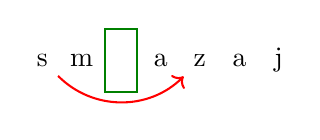
\begin{tikzpicture}
\node (2) at (0.5,0) {s};
\node (3) at (1,0) {m};
\node (4) at (1.5,0) {\textchi};
\node (5) at (2,0) {a};
\node (6) at (2.5,0) {z};
\node (7) at (3,0) {a};
\node (8) at (3.5,0) {j};
\path[->, red] (2) edge[bend right = 45] (6);
\draw[green!50!black] (1.3, -0.4) rectangle (1.7, 0.4);
\end{tikzpicture}
\end{center}
\caption{SP grammar incorrectly rules out Imdlawn Tashlhiyt word \emph{sm\textchi azaj}.}
\label{imdlawnbadsp}
\end{figure}

Increasing the size of the substrings to $3$ will not solve the problem with the blocking effect either.
An SP grammar that finds the word \emph{sm\textchi azaj} correct will inevitably accept all subsequences of that word.
As a result, it would incorrectly predict the well-formedness of the word \emph{smzaj}, where $s$ and $z$ disagree in voicing without the presence of a blocker.



\paragraph{Unbounded tone plateauing}
The ability of SP grammars to see substructures independently of other elements of the string gives them the power to encode \emph{unbounded tone plateauing} (UTP) attested in Luganda (Niger-Congo).
In that language, low tones are realized as high if they are surrounded by high tones \citep{HymanKatamba2010}.
This makes it impossible for a well-formed word in Luganda to have low tones surrounded by high tones, see data in (19) cited by \citep{Hyman2011,Jardine2016}.
Accented vowels indicate high tones, and other vowels are low.

\medskip
\begin{tabular}{llcl}
(19) & bik\'opo byaa-wal\'usiimbi & $\rightarrow$ & bik\'op\'o by\'a\'a-w\'al\'usiimbi \\
& `the cups of Walusimbi' &&
\end{tabular}
\medskip

Using the letters $H$ and $L$ to indicate high and low tones, we can express the generalization as ``never have one or more L in-between two H''.
This allows for strings such as \emph{HHL} and \emph{LLLHHHL}, but prohibits ones such as \emph{HHLLLHH}.
Due to the long-distant nature of SP grammars, a $3$-local SP grammar can capture UTP by ruling out words that contain a subsequence $HLH$, see Figure \ref{imdlawngoodsp}.

\begin{figure}[h!]
\begin{center}

\begin{tikzpicture}
\node (1) at (0,0) {L};
\node (2) at (0.5,0) {L};
\node (3) at (1,0) {H};
\node (4) at (1.5,0) {H};
\node (5) at (2,0) {L};
\node (6) at (2.5,0) {L};
\node (6) at (2.5,-0.3) {\textcolor{white}{L}};
\end{tikzpicture}
\hspace{3em}
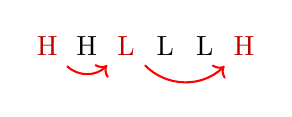
\begin{tikzpicture}
\node (1) at (0,0) {\textcolor{red!75!black}{H}};
\node (2) at (0.5,0) {H};
\node (3) at (1,0) {\textcolor{red!75!black}{L}};
\node (4) at (1.5,0) {L};
\node (5) at (2,0) {L};
\node (6) at (2.5,0) {\textcolor{red!75!black}{H}};
\path[->, red] (1) edge[bend right = 45] (3);
\path[->, red] (3) edge[bend right = 45] (6);
\end{tikzpicture}
\end{center}
\caption{SP grammar captures the UTP pattern.}
\label{imdlawngoodsp}
\end{figure}

{
\renewcommand{\tablename}{Grammar}
\begin{table}[h!]
\begin{center}
\begin{tabular}{rl}
\textit{SP grammar}  & Luganda unbounded tone plateauing \\
\textit{$\Sigma$ =}      &  \{H, L\}   \\
\textit{$R$ =} & $\langle$HLH$\rangle$  \\
\textit{$k$ =}      & $3$          
\end{tabular}
\caption{$3$-SP grammar for Luganda unbounded tone plateauing.}
\label{utpsuccessfulsp}
\end{center}
\end{table}
}

Strictly piecewise grammars capture one or more long-distance processes that do not exhibit blocking effects.
They prohibit subsequences of strings, therefore ruling out all words that contain the illicit substructure.
For example, the restriction $zs$ means that nowhere in the string, $z$ can be followed by $s$.
However, blocking effects cannot be captured via an SP grammar, because the grammar is not sensitive to the presence of the blockers that make the banned substructure acceptable.
Purely short-distant restrictions such as the word-final devoicing also cannot be expressed by an SP grammar: the restriction $b\eow$ prohibits \emph{any} string containing $b$, because $\eow$ always follows $b$ in a word annotated with the word-final marker $\eow$.



\subsubsection{Formal definition}

An SP grammar is defined as a list of subsequences prohibited in well-formed strings of its language.
Further, I define the notion of the subsequence and the SP languages formally following \cite{Rogers-HeinzEtAl-2010-LPTSS}, and then provide an alternative definition in automata-theoretic terms.



\begin{definition}[\textbf{Subsequences}]
A \emph{subsequence} relation $v \sqsubseteq~ w$ is a partial order on the elements of $\Sigma^*$.
A string $v$ is a subsequence of $w$, $v \sqsubseteq~ w$, if $v$ is an empty string, or if $v = \sigma_1\sigma_2\dots\sigma_n$, and there is a collection of substrings $x_1, \dots, w_n \in \Sigma^*$, such that those substrings can be placed between the elements of $v$ thus obtaining $w = w_0\sigma_1 w_1\dots\sigma_n w_n$.

Then all $k$-long subsequences $P_k(w)$ of a word $w \in \Sigma^*$ can be computed as

$$ P_{k}(w) = \{v \in \Sigma^{k} : v \sqsubseteq w\} $$

Similarly, $P_{\leq k}(w)$ lists all subsequences of $w \in \Sigma^*$  of the length up to $k$.

$$ P_{\leq k}(w) = \{v \in \Sigma^{\leq k} : v \sqsubseteq w\} $$
\end{definition}



For example, consider a string $w = abcd$.
Then $P_{3}(w) = \{abc, abd, acd\}$, and $P_{\leq 3}(w) = P_{3}(w) \cup \{\epsilon, a, b, c, d, ab, ac, ad, bc, bd, cd\}$, where $\epsilon$ is the empty string.

\begin{definition}[\textbf{SP languages and grammars}]
A $k$-SP grammar is a pair $\mathcal{G} = \langle \Sigma, S\rangle$ where $S \subseteq \Sigma^k$. The language licensed by a $k$-SP grammar is

\[
	L(\mathcal{G}) = \{w \in \Sigma^* : P_{\leq k}(w) \subseteq P_{\leq k}(T)\}.
\]
\end{definition}

%Consider a $3$-SP grammar with $\Sigma = \{a, o, x\}$, and prohibited substrings $ao$ and $oa$.
%Elements $a$ and $o$ can thus never co-occur within a word, no matter how far away they are from each other, separated by numerous $x$.
The exact reason why SP grammars cannot capture the blocking effect is their \emph{closure under subsequence}; see \citep{Rogers-HeinzEtAl-2010-LPTSS} for other properties of SP languages and grammars.

\begin{definition}[\textbf{Subsequence closure}]
Given a word $w \in L$, all strings $v$ that are subsequences of $w$, $v \sqsubseteq w$, also belong to the language $L$: $v \in L$.
\end{definition}


Alternatively, an SP language can be defined as a deterministic finite automaton (DFA) of a particular shape.
Such a machine is a quintuple $\mathcal{M} = \langle Q, \Sigma, q_0, \delta, F\rangle$, where $Q$ is a finite set of states, $\Sigma$ is the alphabet, $q_0$ is the unique initial state, $\delta$ is the transition function, and $F$ is the set of accepting states.
The following properties are true for the automata recognizing SP languages.
All states of $\mathcal{M}$ are accepting, i.e.\ $F = Q$.
If $q_2$ is reachable from $q_1$ and if there is no transition reading $\sigma \in \Sigma$ from $q_1$, there will be no transition reading $\sigma$ from $q_2$ (missing edges propagate down).
All cycles are self-edges.
If such a machine accepts a string $w\cdot v\cdot u : w, v, u \in \Sigma^{*}$, it necessarily accepts a string $w\cdot u$.
This dependency, however, is not true in the other direction: if such a DFA accepts $w\cdot u$, there could be $v \in \Sigma^*$ such that $w\cdot v\cdot u$ is not an acceptable input sequence.
A DFA with these properties accepts only SP languages.







\subsection{Long-distant dependencies with blocking as TSL languages}


Earlier, I showed that SL and SP grammars cannot capture long-distance harmonies with a blocking effect.
SL grammars can only express local generalizations, and SP restrictions target certain subsequences and therefore are not sensitive to the presence of blockers.
Tier-based strictly local (TSL) grammars capture long-distance dependencies by \emph{making them local} over the tier \citep{HeinzRawal11}.

\subsubsection{Intuitive definition}

I demonstrate the capacities of TSL grammars using the examples of vowel harmony in Karaj\'a (ATR harmony with nasalized blockers) and Buryat (ATR and rounding harmony without blockers).

\paragraph{Karaj\'a vowel harmony}

Consider vowel harmony in Karaj\'a (Macro-J\^e), where a tense vowel spreads the advanced tongue root (ATR) feature leftwards.
It makes it impossible to have a lax vowel followed by a tense one.
This spreading can be blocked by intervening nasalized vowels; they are opaque for this harmony \citep{Ribeiro2002}.


\begin{figure}[h!]
\begin{tabular}{llll}
(20) & woku & {[}woku{]} & `inside' \\
(21) & d\textopeno r\textepsilon & {[}d\textopeno r\textepsilon{]} & `parrot' \\
(22) & bu\texthtd\textepsilon & {[}bu\texthtd\textepsilon{]} & `little, few' \\
(23) & br\textopeno r\textepsilon d$\breve{\imath}$ & {[}broren$\breve{\imath}${]} & `cow (\emph{lit.} deer-similar.to)' \\
(24) & d\textopeno r\textepsilon~ de & {[}dorede{]} & `parrot's wing' \\
(25) & rak\textopeno h\textopeno\texthtd\textepsilon k\~ore & {[}rak\textopeno h\textopeno\texthtd\textepsilon k\~ore{]} & `He/she didn't hit it.' \\
(26) & r\textepsilon b\~\textschwa re & {[}r\textepsilon m\~\textschwa re{]} & `I caught (it).'
\end{tabular}
\end{figure}

The data in (20-26) exemplifies the rule of harmony and is discussed in more detail in \citep{Ribeiro2002}.
Note, that the harmony is reflected in the transcriptions and not in the orthography of the language.
Stems in Karaj\'a can contain tense (20) or lax (21) vowels, and the lax vowels can only follow the tense ones (22).
A tense vowel starts its harmonic domain and spreads the [+ATR] feature regressively (23-24).
However, nasalized vowels such as \emph{\~o} and \~\textschwa~ are opaque for this spreading: they do not enforce the agreement of the vowel thus allowing lax vowels to precede the nasal ones, even if a tense vowel follows it (25-26).

A TSL grammar is defined for a \emph{tier alphabet} $T$ that includes all segments that are relevant for the long-distance dependency.
All vowels are relevant for the harmony, i.e.\ they are either undergoers (lax vowels), or blockers (nasalized vowels), or start the harmonic domain (tense vowels).
Therefore in this case, the tier alphabet contains all vowels, $T = \{$\textepsilon$, o, e, u,$ \textopeno, \emph{\~o}, \~\textschwa~$, a, \dots\}$.
A \emph{tier image} of the string is a representation of that string where only the elements of $T$ are preserved.
For example, the tier image of \emph{rak\textopeno h\textopeno\texthtd\textepsilon k\~ore} is \emph{a\textopeno\textopeno\textepsilon\~oe}.
Finally, the set of restrictions $R$ is defined for the tier representations of the string.
In other words, the prohibited elements are the substrings that must not be observed in the tier representations of well-formed words of the language.

To construct the tier grammar for the Karaj\'a vowel harmony, one needs to prohibit all combinations of a lax vowel followed by a tense one, i.e.\ \textepsilon$e,$ \textepsilon$o,$ \textopeno$o,$ \textopeno$u$, etc.
The presence of the nasalized vowels on the tier allows for sequences such as \textepsilon$\dots$\~\textschwa$\dots e$, where the opaque element blocks spreading of the ATR feature.
Indeed, in such cases, the lax vowel \textepsilon~ and the tense  $e$ are not tier adjacent because of the intervening \~\textschwa.
This makes TSL grammars a good fit for many harmonic patterns, even if they exhibit blocking effects.

{
\renewcommand{\tablename}{Grammar}
\begin{table}[h!]
\begin{center}
\begin{tabular}{rl}
\textit{TSL grammar}  & Karaj\'a vowel harmony in ATR \\
\textit{$\Sigma$ =}      &  \{\textepsilon, \~o, \~\textschwa, o, e, u, \textopeno, a, \~\textschwa, \~a, \~o $\dots$ b, \texthtd, d, r $\dots$\} \\
\textit{$T$ =}      &  \{\textepsilon, \~o, \~\textschwa, o, e, u, \textopeno, a, \~\textschwa, \~a, \~o $\dots$\}  \\
\textit{$R$ =} & $\langle$\textepsilon e, \textepsilon o,  \textopeno o, \textopeno u, \textepsilon u $\dots\rangle$  \\
\textit{$k$ =}      & $2$          
\end{tabular}
\caption{$2$-TSL grammar for Karaj\'a vowel harmony in ATR.}
\label{fdfsdrgr}
\end{center}
\end{table}
}


\begin{figure}[h]
\hspace{0.5em}
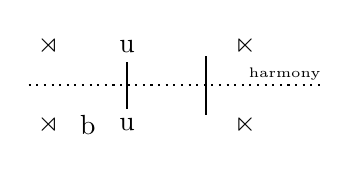
\begin{tikzpicture}
\node (0) at (0,0) {\bow};
\node (1) at (0.5,0) {b};
\node (2) at (1,0) {u};
\node (3) at (1.5,0) {\texthtd};
\node (4) at (2,0) {\textepsilon};
\node (5) at (2.5,0) {\eow};
%
\node (0) at (0,1) {\bow};
\node (02) at (1,1) {u};
\node (04) at (2,1) {\textepsilon};
\node (5) at (2.5,1) {\eow};
%
\foreach \Source/\Target in {%
    2.north/02.south,
	4.north/04.south%
    }
\draw (\Source) to (\Target);
%
\draw[dotted] (-0.25,0.5) to (3.5,0.5);
\node at (3,0.65) {{\tiny harmony}};
\end{tikzpicture}
%
\hspace{2em}
%
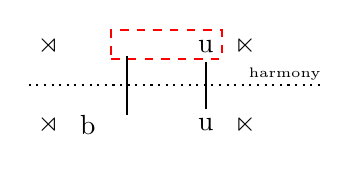
\begin{tikzpicture}
\node (0) at (0,0) {\bow};
\node (1) at (0.5,0) {b};
\node (2) at (1,0) {\textepsilon};
\node (3) at (1.5,0) {\texthtd};
\node (4) at (2,0) {u};
\node (5) at (2.5,0) {\eow};
%
\node (0) at (0,1) {\bow};
\node (02) at (1,1) {\textepsilon};
\node (04) at (2,1) {u};
\node (0) at (2.5,1) {\eow};
%
\foreach \Source/\Target in {%
    2.north/02.south,
	4.north/04.south%
    }
\draw (\Source) to (\Target);
%
\draw[dotted] (-0.25,0.5) to (3.5,0.5);
\node at (3,0.65) {{\tiny harmony}};
\draw [dashed, red] (0.8,0.83) -- (2.2,0.83) -- (2.2,1.2) -- (0.8,1.2) -- (0.8,0.83);
\end{tikzpicture}
%
\hspace{2em}
%
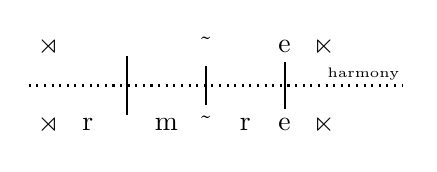
\begin{tikzpicture}
\node (0) at (0,0) {\bow};
\node (1) at (0.5,0) {r};
\node (2) at (1,0) {\textepsilon};
\node (3) at (1.5,0) {m};
\node (4) at (2,0) {\~\textschwa};
\node (5) at (2.5,0) {r};
\node (6) at (3,0) {e};
\node (7) at (3.5,0) {\eow};
%
\node (0) at (0,1) {\bow};
\node (02) at (1,1) {\textepsilon};
\node (04) at (2,1) {\~\textschwa};
\node (06) at (3,1) {e};
\node (0) at (3.5,1) {\eow};
%
\foreach \Source/\Target in {%
    2.north/02.south,
	4.north/04.south,
	6.north/06.south%
    }
\draw (\Source) to (\Target);
%
\draw[dotted] (-0.25,0.5) to (4.5,0.5);
\node at (4,0.65) {{\tiny harmony}};
\end{tikzpicture}
\caption{Evaluation of strings \emph{bu\texthtd\textepsilon}, \emph{b\textepsilon\texthtd u} and \emph{r\textepsilon b\~\textschwa re} by a TSL grammar capturing Karaj\'a vowel harmony in ATR.}
\label{fig:sldkfj}
\end{figure}

See Figure \ref{fig:sldkfj} for the visualization of how the TSL grammar evaluates strings.
The word \emph{bu\texthtd\textepsilon} is well-formed, since the tense vowel is not preceded by any lax vowels, however, \emph{b\textepsilon\texthtd u} contains the violation \textepsilon$u$ and therefore is ruled out.
In \emph{r\textepsilon b\~\textschwa re}, there is a lax vowel followed by a tense one, but there is a blocker \~\textschwa~ in-between them, and its presence on the tier breaks the locality between \textepsilon~ and $e$ therefore allowing such a configuration.

\paragraph{Buryat vowel harmony}
Now, let us consider a type of vowel harmony in Buryat (Mongolian) that spreads both ATR and rounding features.
All vowels within a word must agree in ATR.
Consecutive non-high vowels agree in rounding unless there is an intervening high vowel that blocks this assimilation \citep{Poppe1960}.
The set of transparent items is the same for both agreements: it includes /i/ and all consonants  \citep{HulstSmith87,Skribnik2003,Svantesson2005}.

\medskip
\begin{tabular}{lll}
(27) & \textopeno r-\textopeno:d & `enter-\textsc{perf}' \\
(28) & \textopeno r-\textupsilon:l-a:d & `enter-\textsc{caus-perf}' \\
(29) & to:r-o:d & `wander-\textsc{perf}' \\
(30) & to:r-u:l-e:d & `wander-\textsc{caus-perf}' \\
(31) & m\textopeno rin-\textopeno: & `horse-\textsc{poss}' \\
(32) & o:rin-go: & `group-\textsc{poss}'
\end{tabular}
\bigskip

Examples (27-32) illustrate the harmony using causative and perfective suffixes.
The causative suffix \emph{-\textupsilon:l (-u:l)} has its vowel specified as high, therefore it agrees with the stem only in ATR.
A non-high vowel of the perfective affix \emph{-a:d (-\textopeno:d, -e:d, -o:d)} agrees with the preceding segment in ATR and, if that segment is non-high, in rounding.
In (27), the non-high perfective affix agrees with the non-high root vowel in ATR and rounding: both vowels are lax and rounded.
But adding the high causative affix in-between them, as in (28), results in the blocking of the labial spreading: the perfective affix no longer agrees with the stem in rounding, because they are separated from each other by the intervening high vowel.
Examples (29-30) show the same effect for the tense roots, and (31-32) demonstrate the transparency of the vowel /i/.

All vowels except /i/ harmonize, and therefore in this case, $T = \{a, e,$ \textopeno, $o,$ \textupsilon, $u\}$.
For example, the tier image of \emph{to:ru:le:d} is \emph{oue}.%
\footnote{The length of vowels is ignored since it is not relevant for the rules of the harmony.}
To create a list of tier restrictions, we need to understand what sequences of harmonizing vowels need to be ruled out.
First, such a TSL grammar includes all bigrams where vowels disagree in tense because the tense harmony cannot be blocked by anything.
It rules out $18$ tier restrictions of the type {[}$\alpha$tense{]}{[}-$\alpha$tense{]}, i.e.\ \textopeno$o, o$\textopeno$, $\textupsilon$u, u$\textupsilon, etc.
Then, we enforce the agreement of tier-adjacent non-high vowels by prohibiting bigrams such as {[}$-$high, $\alpha$round{]}{[}$-$high, $-\alpha$round{]}.
It rules out $8$ combinations such as \textopeno$a, a$\textopeno$, eo,$ and others.
Finally, we block rounded vowels from following high vowel, i.e.\ {[}$+$high{]}{[}$-$high, $+$round{]}.
That results in prohibiting \textupsilon\textopeno, $uo, u$\textopeno, and \textupsilon$o$.
In such a way, we encode Buryat vowel harmony in ATR and rounding using a TSL grammar in \ref{buryatvw}.


{
\renewcommand{\tablename}{Grammar}
\begin{table}[h!]
\begin{center}
\begin{tabular}{rl}
\textit{TSL grammar}  & Buryat vowel harmony in ATR and rounding \\
\textit{$\Sigma$ =}      &  \{a, b, t, o, \textopeno, e, d, l, $\dots$\}   \\
\textit{$T$ =}      &  \{a, e, \textopeno, o, \textupsilon, u\}  \\
\textit{$R$ =} & $\langle$\textopeno o, o\textopeno,  \textupsilon u, u\textupsilon $\dots$ \textopeno a, a\textopeno, eo, oe, ao $\dots$ \textupsilon\textopeno, uo, u\textopeno,  \textupsilon o$\rangle$  \\
\textit{$k$ =}      & $2$          
\end{tabular}
\caption{$2$-TSL grammar for Buryat vowel harmony in ATR and rounding.}
\label{buryatvw}
\end{center}
\end{table}
}


Figure \ref{fig:bur} shows that the tier images of \emph{to:ro:d} and \emph{to:ru:le:d} are \emph{oo} and \emph{oue}, respectively.
These tiers are well-formed: both words are tense, and in both cases, the second vowel inherits its rounding feature from the first non-high vowel, however, its value cannot be passed from a high vowel to a non-high one.
The word \emph{to:re:d} is illicit since its tier image \emph{oe} is prohibited: vowels must agree with the preceding non-high vowel in rounding.
The form \emph{to:ru:l\textopeno:s} is also ruled out, since its tier \emph{ou\textopeno} contains the prohibited bigram $u$\textopeno, since \textopeno~ cannot inherit its rounding value from the preceding high vowel $u$, and they also disagree in ATR.
In such a way, TSL grammar captures a pattern where a certain set of elements exhibits a long-distance dependency.


\begin{figure}[h]
\hspace{7em}
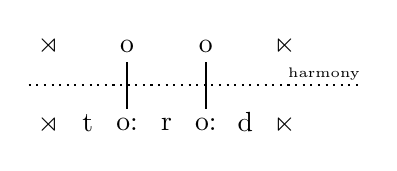
\begin{tikzpicture}
\node (f) at (-0.5, 0) {\bow};
\node (0) at (0,0.027) {t};
\node (1) at (0.5,0) {o:};
\node (2) at (1,0) {r};
\node (3) at (1.5,0) {o:};
\node (4) at (2,0.04) {d};
\node (f) at (2.5, 0) {\eow};
%
\node (f) at (-0.5, 1) {\bow};
\node (01) at (0.5,1) {o};
\node (03) at (1.5,1) {o};
\node (f) at (2.5, 1) {\eow};
%
\foreach \Source/\Target in {%
        1.north/01.south,
	3.north/03.south%
    }
\draw (\Source) to (\Target);
%
\draw[dotted] (-0.75,0.5) to (3.5,0.5);
\node at (3,0.65) {{\tiny harmony}};
\end{tikzpicture}
%
\hspace{5em}
%
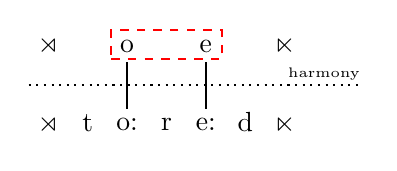
\begin{tikzpicture}
\node (f) at (-0.5, 0) {\bow};
\node (0) at (0,0.027) {t};
\node (1) at (0.5,0) {o:};
\node (2) at (1,0) {r};
\node (3) at (1.5,0) {e:};
\node (4) at (2,0.04) {d};
\node (f) at (2.5, 0) {\eow};
%
\node (f) at (-0.5, 1) {\bow};
\node (01) at (0.5,1) {o};
\node (03) at (1.5,1) {e};
\node (f) at (2.5, 1) {\eow};
%
\foreach \Source/\Target in {%
        1.north/01.south,
	3.north/03.south%
    }
\draw (\Source) to (\Target);
%
\draw[dotted] (-0.75,0.5) to (3.5,0.5);
\node at (3,0.65) {{\tiny harmony}};
\draw [dashed, red] (0.3,0.83) -- (1.7,0.83) -- (1.7,1.2) -- (0.3,1.2) -- (0.3,0.83);
\end{tikzpicture}\vspace{0.5em}

\hspace{5em}
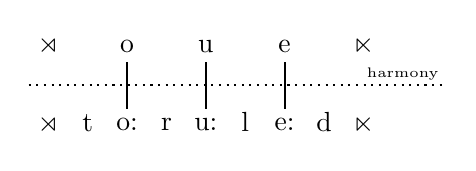
\begin{tikzpicture}
\node (f) at (-0.5, 0) {\bow};
\node (0) at (0,0.027) {t};
\node (1) at (0.5,0) {o:};
\node (2) at (1,0) {r};
\node (3) at (1.5,0) {u:};
\node (4) at (2,0.04) {l};
\node (5) at (2.5,0) {e:};
\node (6) at (3,0.04) {d};
\node (f) at (3.5, 0) {\eow};
%
\node (f) at (-0.5, 1) {\bow};
\node (01) at (0.5,1) {o};
\node (03) at (1.5,1) {u};
\node (05) at (2.5,1) {e};
\node (f) at (3.5, 1) {\eow};
%
\foreach \Source/\Target in {%
        1.north/01.south,
        3.north/03.south,
	5.north/05.south%
    }
\draw (\Source) to (\Target);
%
\draw[dotted] (-0.75,0.5) to (4.5,0.5);
\node at (4,0.65) {{\tiny harmony}};
%
%\node at (0.4,1.5) {$^{ok}$to:ru:le:d};
\end{tikzpicture}
%
\hspace{3em}
%
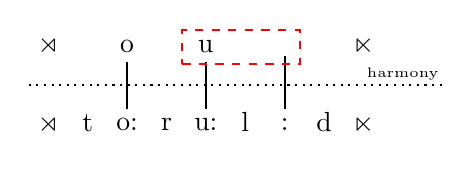
\begin{tikzpicture}
\node (f) at (-0.5, 0) {\bow};
\node (0) at (0,0.027) {t};
\node (1) at (0.5,0) {o:};
\node (2) at (1,0) {r};
\node (3) at (1.5,0) {u:};
\node (4) at (2,0.04) {l};
\node (5) at (2.5,0) {\textopeno:};
\node (6) at (3,0.04) {d};
\node (f) at (3.5, 0) {\eow};
%
\node (f) at (-0.5, 1) {\bow};
\node (01) at (0.5,1) {o};
\node (03) at (1.5,1) {u};
\node (05) at (2.5,1) {\textopeno};
\node (f) at (3.5, 1) {\eow};
%
\foreach \Source/\Target in {%
        1.north/01.south,
        3.north/03.south,
	5.north/05.south%
    }
\draw (\Source) to (\Target);
%
\draw[dotted] (-0.75,0.5) to (4.5,0.5);
\node at (4,0.65) {{\tiny harmony}};
\draw [dashed, red] (1.2,0.77) -- (2.7,0.77) -- (2.7,1.2) -- (1.2,1.2) -- (1.2,0.77);
%
%\node at (0.4,1.5) {*to:ru:lo:d};
\end{tikzpicture}
\caption{Evaluation of strings \emph{to:ro:d}, \emph{to:ru:le:d}, \emph{to:re:d} and \emph{to:ru:l\textopeno:s} by a TSL grammar capturing Buryat vowel harmony in ATR and rounding.}
\label{fig:bur}
\end{figure}

Apart from the long-distant patterns, TSL grammars can easily capture local dependencies since they are a proper extension of SL languages, see section \ref{subgsgf}.
If a purely local dependency such as obstruent word-final devoicing or obstruent cluster voicing assimilation is expressed via a TSL grammar, its tier alphabet $T$ will be the same as $\Sigma$.

As of the patterns discussed above, the Tuareg sibilant harmony in voicing and anteriority can also be described by a TSL grammar.
In this case, the tier includes all sibilants.
However, a similar harmony of Imdlawn Tashlhiyt, where only the voicing assimilation can be blocked by voiced obstruents, is not TSL.
The anteriority harmony cannot be blocked, and the appearance of the voiced obstruents on the tier would break the locality relation between the sibilants.
The absence of the voiceless obstruents on the tier, however, makes it impossible to model the blocking of the voicing harmony.
This creates two sets of items involved in a long-distance dependency: sibilants that are relevant for the anteriority harmony, and both sibilants and voiceless obstruents that are involved in the voicing harmony.
It would thus require two tiers to capture the Imdlawn Tashlhiyt pattern; see \cite{McMullin2016} and \cite{AksenovaDeshmukh2018} for the discussion of harmonies in more than a single feature, and tier properties of those harmonies.

Similarly, it is impossible to express a UTP generalization ``no low tones in-between high tones'' using a TSL grammar.
Both L and H tones are important for the pattern, but including them both on the tier would make it impossible to notice the HLH configuration: the presence of the additional Ls, such as in \emph{HHLLLLLLH}, makes the dependency non-local.


To sum up, TSL languages capture long-distance dependencies that can potentially include blocking or licensing effects.
However, several long-distant assimilations cannot be expressed by a single TSL grammar if they affect different sets of segments.

\subsubsection{Formal definition}

TSL languages are a proper extension of the SL ones, but the $k$-local constraints are imposed on the \emph{tier} symbols $T \subseteq \Sigma$.
\cite{DeSantoGraf19FG} define tier-locality using the notion of the \emph{erasing function} $E$, also called the \emph{projection function}.
Its purpose is to delete all symbols that are not included in the tier alphabet $T$.
Given some string $\sigma \in \Sigma$, the erasing function $E_{T}$ maps $\sigma$ to itself if $\sigma \in T$ and to $\epsilon$ otherwise.
In such a way, under the erasing function, a tier image of a word $w = \sigma_0\dots\sigma_n$ is obtained by substituting non-tier elements $\sigma \not\in T$ by $\epsilon$.


\begin{definition}[\textbf{TSL languages and grammars}]
A language $L$ is \emph{tier-based strictly $k$-local} ($k$-TSL) iff there exists a tier $T \subseteq \Sigma$ and a finite set $S \subseteq F_k(\rtimes^{k-1} T^* \ltimes^{k-1})$ such that
\[
L = \{ w \in \Sigma^* :   F_k(\rtimes^{k-1} E_T(w) \ltimes^{k-1})  \cap S = \emptyset \}
\]
Additionally, $S$ the set of forbidden $k$-factors on tier $T$, and $\langle T, S\rangle$ is a $k$-TSL grammar.
\end{definition}

\cite{DeSantoGraf19FG} show that a language $L$ is TSL iff it is strictly $k$-local on tier $T$ for some $T \subseteq \Sigma$ and $k \in \mathbb{N}$.
Indeed, SL properties such as suffix substitution closure (see the definitions in \ref{suffsubclosure}) can be generalized, as it was done by \cite{LambertRogers2020}.
For example, a language $x^*a^*x^*b^*x^*$ is not SL since it is not closed under suffix substitution.
However, if only $a$ and $b$ are included in the tier alphabet, it becomes $2$-TSL, with the shape of the tier restricted to $a^*b^*$. 



In their paper, \cite{LambertRogers2020} show how to construct a DFA for a given TSL grammar.
Namely, they start by encoding every allowed $k$-TSL factor in its own automaton, uniting all the automata obtained this way, and then adding loops reading non-tier symbols to every state.
In such a way, a TSL-representing DFA is a DFA expressing the local restrictions on the tier symbols, and looping on the non-tier ones.







\subsection{Multiple long-distant dependencies with blocking as MTSL languages}

Multi-tier strictly local (MTSL) grammars are conjunction of several TSL grammars.
A language of an MTSL grammar is the intersection of languages of multiple TSL grammars \citep{DeSantoGraf19FG}.
An MTSL grammar lists $k$ tier alphabets $T_1 \dots T_k$, and for every tier alphabet $T_i$, there is a corresponding set of restrictions $R_i$.
A string is well-formed with respect to a given MTSL grammar if it is well-formed on every tier.



\subsubsection{Intuitive definition}

Imdlawn Tashlhiyt sibilant harmony exhibits a blocking effect for only one feature out of two that are spreading (voicing and anteriority).
In this subsection, I show that this pattern is MTSL.

\paragraph{Imdlawn Tashlhiyt}
Consider the regressive sibilant harmony in Imdlawn Tashlhiyt discussed earlier in 2.1.4.
Sibilants in that language agree in voicing and anteriority.
For example, in \emph{zbruz:a} `\textsc{caus}-crumble', both sibilants are voiced and anterior, and in \emph{sas:twa} `\textsc{caus}-settle', they are voiceless and anterior, in \emph{\textesh fia\textesh r} `\textsc{caus}-be.full.of.straw', they are voiceless and non-anterior.
However, while the anteriority harmony cannot be blocked by anything, the voicing harmony can be blocked by intervening voiceless obstruents such as \textchi, $k$ or $q$, resulting in the well-formedness of words such as \emph{sm\textesh azaj} `\textsc{caus}-loathe.each.other'.

This pattern is not SL, SP or TSL.
It is not SL since it involves a long-distance dependency.
An SP grammar cannot capture it either because it cannot model blockers.
A TSL grammar is not a good fit either: both sibilants and voiceless obstruents need to be present on the tier to express the voicing harmony; however, the presence of non-sibilants on the tier breaks the tier locality required to model the anteriority assimilation.
More than a single tier is required to model this generalization.

The power of MTSL grammars allows projecting multiple tiers, and this helps to model the Imdlawn Tashlhiyt pattern.
Sibilants and voiceless obstruents are projected on one tier, let us call it $T_{voice}$, whereas only sibilants are visible on the second tier $T_{ant}$.
The tier capturing the voicing harmony restricts all combinations of sibilants disagreeing in voicing ($sz$, $zs$, \textesh\textyogh, \textyogh\textesh), and also voiced sibilants followed by voiceless obstruents ($zk$, $zf$, $z$\textchi, etc.).
On the tier of anteriority, the combinations of sibilants of different anteriority are not allowed ($s$\textesh, $z$\textesh, \textesh$s$, etc.).
The obtained grammar is summarized in \ref{imdlawnmtsl}.

{
\renewcommand{\tablename}{Grammar}
\begin{table}[h!]
\begin{center}
\begin{tabular}{rl}
\textit{MTSL grammar}  & Imdlawn Tashlhiyt sibilant harmony in voicing and anteriority \\
\textit{$\Sigma$ =}      &  \{a, b, m, u, g, r, s, z, \textesh, \textyogh, \textcrh, k, f, \textchi, q, $\dots$\}   \\
\textit{$T_{ant}$ =}      &  \{s, z, \textesh, \textyogh\}  \\
\textit{$R_{ant}$ =} & \{s\textesh, z\textesh, \textesh s, \textesh z, s\textyogh, z\textyogh, \textyogh s, \textyogh z\}  \\
\textit{$T_{voice}$ =}      &  \{s, z, \textesh, \textyogh, \textcrh, k, f, \textchi, q\}  \\
\textit{$R_{voice}$ =} & \{sz, zs, \textesh\textyogh, \textyogh\textesh, z\textcrh, zk, zf, z\textchi, zq, \textyogh\textcrh, \textyogh k, \textyogh f, \textyogh\textchi, \textyogh q\}  \\
\textit{$k$ =}      & $2$          
\end{tabular}
\caption{$2$-MTSL grammar for Imdlawn Tashlhiyt sibilant harmony in voicing and anteriority.}
\label{imdlawnmtsl}
\end{center}
\end{table}
}

This MTSL grammar correctly models the generalization behind the Imdlawn Tashlhiyt pattern.
Ill-formed strings such as \emph{\textyogh bruz:a} are illicit because the tier of the anteriority harmony contains a prohibited bigram \textyogh$z$.
The combinations of sibilants that agree in voicing are allowed on that tier, and it is the case in well-formed words such as \emph{sm\textesh azaj}, where \textesh~ blocks the voicing agreement.
Voiced sibilants cannot precede voiceless obstruents, so forms such as \emph{zm\textesh azaj} are ruled out on the tier of voicing by the restriction $z$\textesh.
Figure \ref{fig:imdlwnpicture} visualizes the discussed examples.


\begin{figure}[h]
\centering
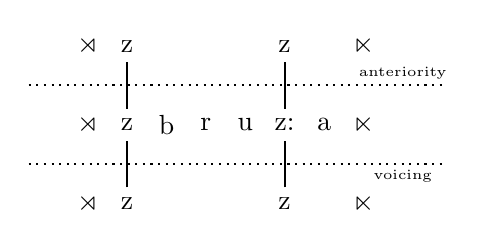
\begin{tikzpicture}
\node (f) at (0, 0) {\bow};
\node (0) at (0.5,0) {z};
\node (1) at (1,0) {b};
\node (2) at (1.5,0) {r};
\node (3) at (2,0) {u};
\node (4) at (2.5,0) {z:};
\node (5) at (3,0) {a};
\node (f) at (3.5, 0) {\eow};
%
\node (f) at (0, 1) {\bow};
\node (00) at (0.5,1) {z};
\node (04) at (2.5,1) {z};
\node (f) at (3.5, 1) {\eow};
%
\node (f) at (0, -1) {\bow};
\node (000) at (0.5,-1) {z};
\node (004) at (2.5,-1) {z};
\node (f) at (3.5, -1) {\eow};
%
\foreach \Source/\Target in {%
        0.north/00.south,
        4.north/04.south,
        000.north/0.south,
        004.north/4.south%
    }
\draw (\Source) to (\Target);
%
\draw[dotted] (-0.75,0.5) to (4.5,0.5);
\node at (4,0.65) {{\tiny anteriority}};
\draw[dotted] (-0.75,-0.5) to (4.5,-0.5);
\node at (4,-0.65) {{\tiny voicing}};
\end{tikzpicture}
%
\hspace{3em}
%
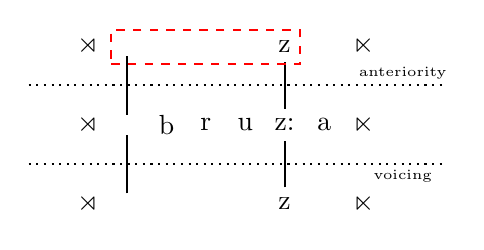
\begin{tikzpicture}
\node (f) at (0, 0) {\bow};
\node (0) at (0.5,0) {\textyogh};
\node (1) at (1,0) {b};
\node (2) at (1.5,0) {r};
\node (3) at (2,0) {u};
\node (4) at (2.5,0) {z:};
\node (5) at (3,0) {a};
\node (f) at (3.5, 0) {\eow};
%
\node (f) at (0, 1) {\bow};
\node (00) at (0.5,1) {\textyogh};
\node (04) at (2.5,1) {z};
\node (f) at (3.5, 1) {\eow};
%
\node (f) at (0, -1) {\bow};
\node (000) at (0.5,-1) {\textyogh};
\node (004) at (2.5,-1) {z};
\node (f) at (3.5, -1) {\eow};
%
\foreach \Source/\Target in {%
        0.north/00.south,
        4.north/04.south,
        000.north/0.south,
        004.north/4.south%
    }
\draw (\Source) to (\Target);
%
\draw[dotted] (-0.75,0.5) to (4.5,0.5);
\node at (4,0.65) {{\tiny anteriority}};
\draw[dotted] (-0.75,-0.5) to (4.5,-0.5);
\node at (4,-0.65) {{\tiny voicing}};
\draw [dashed, red] (0.3,0.77) -- (2.7,0.77) -- (2.7,1.2) -- (0.3,1.2) -- (0.3,0.77);
\end{tikzpicture}

\vspace{1.5em}

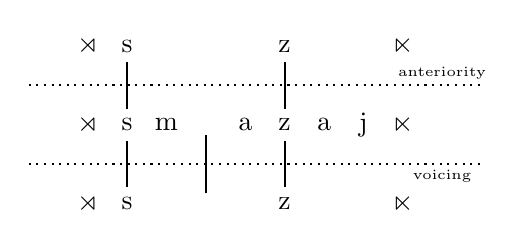
\begin{tikzpicture}
\node (f) at (0, 0) {\bow};
\node (0) at (0.5,0) {s};
\node (1) at (1,0) {m};
\node (2) at (1.5,0) {\textchi};
\node (3) at (2,0) {a};
\node (4) at (2.5,0) {z};
\node (5) at (3,0) {a};
\node (6) at (3.5, 0) {j};
\node (f) at (4, 0) {\eow};
%
\node (f) at (0, 1) {\bow};
\node (00) at (0.5,1) {s};
\node (04) at (2.5,1) {z};
\node (f) at (4, 1) {\eow};
%
\node (f) at (0, -1) {\bow};
\node (000) at (0.5,-1) {s};
\node (002) at (1.5,-1) {\textchi};
\node (004) at (2.5,-1) {z};
\node (f) at (4, -1) {\eow};
%
\foreach \Source/\Target in {%
        0.north/00.south,
        4.north/04.south,
        000.north/0.south,
        002.north/2.south,
        004.north/4.south%
    }
\draw (\Source) to (\Target);
%
\draw[dotted] (-0.75,0.5) to (5,0.5);
\node at (4.5,0.65) {{\tiny anteriority}};
\draw[dotted] (-0.75,-0.5) to (5,-0.5);
\node at (4.5,-0.65) {{\tiny voicing}};
\end{tikzpicture}
%
\hspace{3em}
%
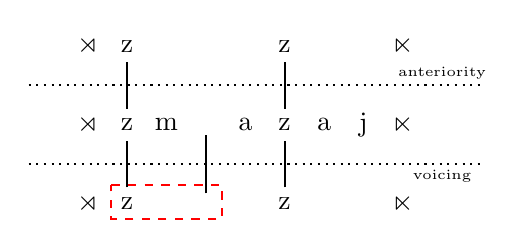
\begin{tikzpicture}
\node (f) at (0, 0) {\bow};
\node (0) at (0.5,0) {z};
\node (1) at (1,0) {m};
\node (2) at (1.5,0) {\textchi};
\node (3) at (2,0) {a};
\node (4) at (2.5,0) {z};
\node (5) at (3,0) {a};
\node (6) at (3.5, 0) {j};
\node (f) at (4, 0) {\eow};
%
\node (f) at (0, 1) {\bow};
\node (00) at (0.5,1) {z};
\node (04) at (2.5,1) {z};
\node (f) at (4, 1) {\eow};
%
\node (f) at (0, -1) {\bow};
\node (000) at (0.5,-1) {z};
\node (002) at (1.5,-1) {\textchi};
\node (004) at (2.5,-1) {z};
\node (f) at (4, -1) {\eow};
%
\foreach \Source/\Target in {%
        0.north/00.south,
        4.north/04.south,
        000.north/0.south,
        002.north/2.south,
        004.north/4.south%
    }
\draw (\Source) to (\Target);
%
\draw[dotted] (-0.75,0.5) to (5,0.5);
\node at (4.5,0.65) {{\tiny anteriority}};
\draw[dotted] (-0.75,-0.5) to (5,-0.5);
\node at (4.5,-0.65) {{\tiny voicing}};
\draw [dashed, red] (0.3,-0.77) -- (1.7,-0.77) -- (1.7,-1.2) -- (0.3,-1.2) -- (0.3,-0.77);
\end{tikzpicture}
\caption{Evaluation of strings \emph{zbruz:a}, \emph{\textyogh bruz:a}, \emph{sm\textesh azaj} and \emph{zm\textesh azaj} by a MTSL grammar capturing Imdlawn Tashlhiyt sibilant harmony in voicing and anteriority.}
\label{fig:imdlwnpicture}
\end{figure}

MTSL grammars model several agreements within the same language, even when they target different sets of segments.
Interestingly, those sets are either in the set-subset relation, or are disjoint, but never only partially overlap.
Imdlawn Tashlhiyt discussed in this section is an example of a harmony where the tier alphabets are in the set-subset relation.
In Bukusu (Bantu), vowels agree in height along with the assimilation of nasals in height, therefore exemplifying the case of the disjoint tier alphabets \citep{Odden1994,Elmedlaoui1995,Hansson2010}.
\cite{AksenovaDeshmukh2018} summarize this restriction and propose its possible explanation.


\subsubsection{Formal definition}

The language at the intersection of several TSL grammars can be viewed as a single grammar projecting multiple tiers, i.e.\ a multi-TSL, or MTSL grammar \citep{DeSantoGraf19FG}.

\begin{definition}[\textbf{MTSL languages}]
An $n$-tier strictly $k$-local ($n$-MTSL$_k$) language $L$ is the intersection of $n$ distinct $k$-TSL languages ($k,n \in \mathbb{N}$).
\end{definition}

Since the language of an MTSL grammar is the intersection of several TSL languages, one can imagine a construction of the corresponding DFA by intersecting several DFAs representing those TSL languages.
According to \cite{LambertRogers2020}, it is possible to create DFAs for any languages definable by Boolean combinations of SL, SP, and TSL automata.
Consequently, it includes MTSL languages.










\subsection{Models of well-formedness conditions: summary}

Subregular grammars describe well-formedness conditions imposed on words in natural languages.
In this section, I focused on SL, SP, TSL, and MTSL grammars since they capture a vast majority of phonological patterns.
SL grammars capture only local processes, therefore they are a good fit for word-final devoicing and obstruent cluster voicing assimilation.
SP grammars generalize long-distance dependencies by prohibiting certain orders of elements, thus they are a good fit for harmonies without blockers and unbounded tone plateauing.
Only a certain subset of elements of the alphabet is projected on a tier by TSL grammars, therefore they capture a long-distance process locally by ignoring irrelevant segments.
This allows them to model a harmony process that can potentially involve blockers.
Finally, MTSL grammars project several tiers, and this helps to represent several independent yet simultaneous harmonies. 
In such a way, these subregular grammars can capture most of the dependencies imposed by phonological well-formedness conditions.

Some known natural language patterns, however, require powers of different subregular language classes.
Among them, there is a pattern of Sanskrit /n/-retroflexion and Yaka harmony triggered by local conditions \citep{Walker2000,McMullin2016,Karakas2020}.
IO-TSL and IBSP subregular language classes can models those cases \citep{Graf17Phonology,Graf18NELS}.
Interestingly, none of the subregular language classes mentioned above can express such theoretically possible but unattested patterns as first-last harmony, where the first vowel of the word needs to harmonize with the last one \citep{Lai15,Avcu2018}.


Later, in chapter 3 of this dissertation, I discuss several subregular patterns and show how the corresponding grammars can be learned from the real data.










\section{Modeling transformations}

The previous section explored modeling of natural language well-formedness conditions using subregular languages.
Here, I discuss formalizing and modeling \emph{transformations}, or rewrite rules, that apply to underlying representations and yield corresponding surface forms.
Namely, I show that subsequential finite-state \emph{transducers} can be employed to model transformations, and discuss their sub-types.
Subsequential mappings belong to a class of regular functions, and therefore subsequential functions are also subregular.

\subsection{Formalizing transformations}
\label{FSTforburyat}

Earlier in Section 2.1.5, I discussed Buryat progressive vowel harmony in ATR and rounding.
Vowels agree in these two features, while consonants and /i/ are transparent.
While all harmonizing vowels are undergoers for the ATR agreement, high vowels \textupsilon~ and $u$ block the spreading of the rounding feature, thus prohibiting the appearance of \textopeno~ and $o$.
So, for example, all vowels in a word \emph{to:r-u:l-e:d} `wander-\textsc{caus-perf}' are tense, and the high vowel $u$ blocks spreading of the rounding feature.
In \emph{to:r-o:d} `wander-\textsc{perf}', all vowels are low, and therefore they agree in rounding as well.
Values of non-initial vowels only depend on their height and the value of the previous vowel.

Now, consider this harmony as a set of pairs exemplifying the mapping from the underlying representations (UR) to the surface forms (SF), see data in (33-38).

\begin{figure}[h]
\begin{tabular}{llcll}
 &  UR &$\rightarrow$ & SF & \\
(33) &  \textopeno r-\textbf{L:}d &$\rightarrow$ & \textopeno r-\textopeno:d & `enter-\textsc{perf}' \\
(34) & \textopeno r-\textbf{H:}l-\textbf{L:}d & $\rightarrow$ & \textopeno r-\textupsilon:l-a:d & `enter-\textsc{caus-perf}' \\
(35) &  to:r-\textbf{L:}d &$\rightarrow$ &  to:r-o:d & `wander-\textsc{perf}' \\
(36) &  to:r-\textbf{H:}l-\textbf{L:}d & $\rightarrow$ & to:r-u:l-e:d & `wander-\textsc{caus-perf}' \\
(37) &  m\textopeno rin-\textbf{L:} & $\rightarrow$ & m\textopeno rin-\textopeno: & `horse-\textsc{poss}' \\
(38) & o:rin-g\textbf{L:} & $\rightarrow$ & o:rin-go: & `group-\textsc{poss}'
\end{tabular}
\end{figure}


A UR of the initial vowel is fully specified, whereas all non-initial vowels are only specified for the height, and therefore are denoted as \textbf{L}ow or \textbf{H}igh.
To obtain the SFs, all $L$ and $H$ of the URs need to be substituted starting from the leftmost one.
The rules of this substitution are listed below.
\bigskip

$L = 
\left\{
\begin{tabular}{@{}l@{}}
    \textrm{`\textopeno' if the previous harmonizing vowel is `\textopeno'} \\
    \textrm{`a' if the previous harmonizing vowel is `a' or `\textupsilon'} \\
    \textrm{`o' if the previous harmonizing vowel is `o'} \\
    \textrm{`e' if the previous harmonizing vowel is `e' or `u'}
\end{tabular}
\right\}$

\bigskip

$H = 
\left\{
\begin{tabular}{@{}l@{}}
    \textrm{`\textupsilon' if the previous harmonizing vowel is `\textopeno', `a' or `\textupsilon'} \\
    \textrm{`u' if the previous harmonizing vowel is `o', `e' or `u'}
\end{tabular}
\right\}$

\bigskip

Previously, Section 2.1.1 introduced finite-state automata (FSA) that are defined via a finite number of states and transitions between them.
Those transitions are annotated with symbols, and strings are read by following the corresponding transitions.
If such transitions exist and the last portion of the string brings the machine to the final state, the string is \emph{accepted}, i.e.\ considered well-formed with respect to the rules encoded by the FSA.
Otherwise, the string is \emph{rejected}.
In such a way, an FSA reads a string and evaluates its well-formedness.

The transitions of the FSA have the following shape: $q_{a}\xrightarrow{\text{b}}q_{b}$.
Such a transition indicates that after reading $b$, the FSA will move from the state $q_{a}$ to $q_{b}$.
The core difference of a \textbf{finite-state transducer} (FST) is that it can \emph{write} an output string while reading the input string \citep{Schuetzenberger1961}.
Transitions of the FST indicate what portion of the input is read, and what is added to the output string, also called the \emph{translation}.
For example, the transition $q_{a}\xrightarrow{\text{b:x}}q_{b}$ means ``to go from $q_{a}$ to $q_{b}$, read $b$ and write $x$''.
Consider a simple example of an FST in Figure \ref{fig:transabcd}.
While FSAs are functions mapping \emph{strings to boolean values}, FSTs map \emph{strings to strings}.


\begin{figure}[h!] 
\centering
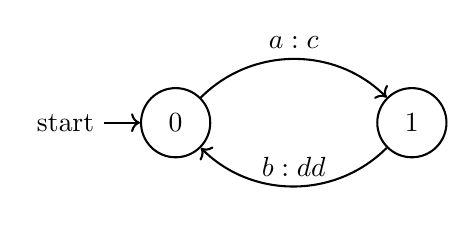
\begin{tikzpicture}
\node[state, initial]  at (0,0) (q0) {$0$};
\node[state] at (3,0) (q1) {$1$};
\path[->] (q0) edge[above,bend left = 45] node{$a:c$} (q1)
	(q1) edge[above,bend left = 45] node{$b:dd$} (q0);
\end{tikzpicture}
\caption{An example of the FST.}
\label{fig:transabcd}
\end{figure}

A transducer in Figure \ref{fig:transabcd} accepts strings that start with $a$ and alternate $a$ and $b$.
Every time $a$ is read, $c$ is written, and every time $b$ is read, $dd$ is written.
It translates \emph{aba} as \emph{cddc}, and \emph{abab} as \emph{cddcdd}.
I employ \textbf{rational} transducers in which all states can be final.


We can construct an FST mapping Buryat URs to the corresponding SFs, as depicted in Figure \ref{buryattransducera}.
For simplicity, $N$ represents all elements that are not involved in the harmony -- consonants and the transparent vowel /i/.
Such a transducer has $5$ states, with $q_0$ being the initial state.
Every state has a loop $N$:$N$ on it, and it means that the irrelevant symbols for the harmony are left as is and do not move the machine to another state.
If the initial vowel is $e$ or $u$, it moves the machine to state $q_1$, and all the following low and high vowels are rewritten as $e$ and $u$, respectively.
If the initial vowel is $o$, state $q_2$ is activated, so all the following low vowels agree in tense and rounding, and therefore are realized as $o$.
However, reading a high vowel $u$ moves the machine to $q_1$ thus blocking the rounding spreading.
States $q_3$ and $q_4$ similarly encode the rounding harmony for lax stems.
In such a way, the transducer in Figure \ref{buryattransducera} takes a Buryat UR as input and returns the corresponding SF as output, where the underspecified segments $H$ and $L$ are rewritten with respect to the rules of the harmony.


\begin{figure}[h!] 
\centering
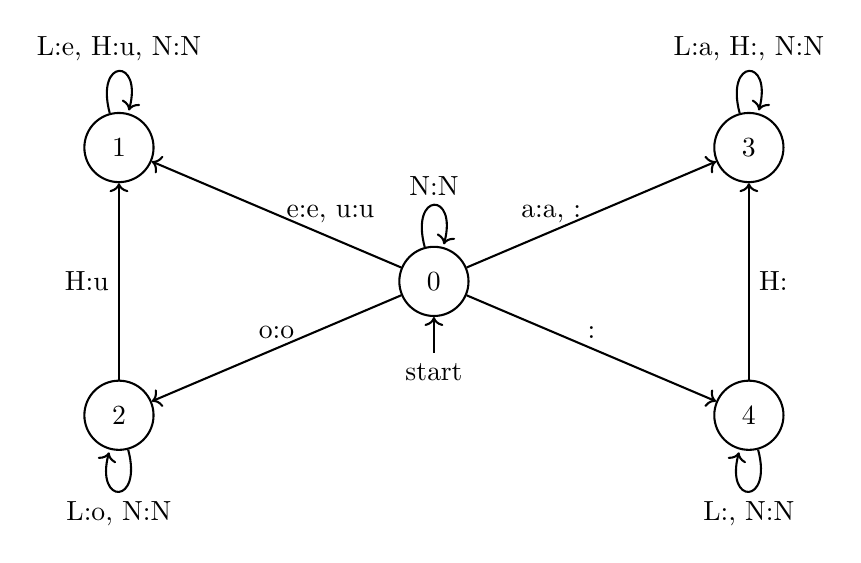
\begin{tikzpicture}
\node[state, initial below]  at (0,0) (q0) {$0$};
\node[state] at (4,1.7) (q1) {$3$};
\node[state] at (4,-1.7) (q2) {$4$};
\node[state] at (-4,1.7) (q3) {$1$};
\node[state] at (-4,-1.7) (q4) {$2$};
\path[->]
	(q0) edge[loop above] node{N:N} (q0)
	(q1) edge[loop above] node{L:a, H:\textupsilon, N:N} (q1)
	(q3) edge[loop above] node{L:e, H:u, N:N} (q3)
	(q2) edge[loop below] node{L:\textopeno, N:N} (q2)
	(q4) edge[loop below] node{L:o, N:N} (q4)
	(q0) edge[left] node{a:a, \textupsilon:\textupsilon} (q1)
	(q0) edge[above] node{\textopeno:\textopeno} (q2)
	(q0) edge[right] node{e:e, u:u} (q3)
	(q0) edge[above] node{o:o} (q4)
	(q4) edge[left] node{H:u} (q3)
	(q2) edge[right] node{H:\textupsilon} (q1);
\end{tikzpicture}
\caption{Transducer for Buryat vowel harmony.}
\label{buryattransducera}
\end{figure}

For example, assume that the word \emph{\textopeno r\textbf{L}d} is given as input.
The initial \textopeno~ brings the machine to the state $q_4$, and $r$ is rewritten as $r$ because of the loop annotated with $N$:$N$.
The following $L$ is now specified: the reflexive loop on the state $q_4$ changes its value to \textopeno.
Finally, $d$ is left without modifications.
The FST in \ref{buryattransducera} rewrites that input form as \emph{\textopeno r\textopeno d} and it is indeed the expected output, see the example (33).
Alternatively, consider the UR \emph{tor\textbf{H}l\textbf{L}d}.
The initial vowel $o$ brings the machine to the state $q_2$, meaning that all the consecutive vowels will be tense.
The following underspecified vowel is high, so it is rewritten as $u$.
Reading that high vowel moves the FST to $q_1$.
The spreading of the rounding feature is blocked, and given that the following vowel is low, it is realized as $e$.
This results in the translation \emph{toruled}, and the example (36) confirms it.
In such a way, FSTs model phonological processes that change URs to the corresponding SFs.





\subsection{Subsequential mappings}
\label{RussianWFDFST}

In line with the regularity of languages satisfying the well-formedness conditions, phonological mappings are also regular \citep{Johnson1972,Koskenniemi1983,KaplanKay94}.
A \emph{regular mapping} is one that can be represented using a FST, similarly to the way the pattern of Buryat vowel harmony is represented as a FST in figure \ref{buryattransducera}.


Similar to the results discussed in the previous sections, resent research shows that phonological mappings also do not require a full power of regular languages.
Instead, subsequential mappings including input and output strictly local transformations were shown to be a good fit for natural language phonological and morphological processes \citep{Chandlee2014,ChandleeHeinz2018}.
Therefore, here, as well as in Chapter 4, I focus on \emph{subsequential transducers} representing subsequential mappings.


The term ``subsequential'', however, can be confusing.
It can be interpreted as \emph{is below sequential} or \emph{subsumes sequential}, and is used in the literature in both of these meanings.
Here following \cite{RocheSchabes1997} and  \cite{DeLaHiguera2010}, I use ``subsequential'' to mean a subclass of sequential machines.
A \textbf{sequential} FST reads symbols of the input string one by one.
Crucially, for every input symbol, there is at most one transition outgoing from any state of such FST that reads that symbol.
Additionally, \textbf{subsequential} machines implement a \emph{state outputting function} that allows for the final portion of the translation to be generated at the end of the parse, depending on the state in which the FST stopped after reading the last input symbol.

In Section \ref{russianwfdpatternn}, I described the pattern of word-final devoicing in Russian, where voiced obstruents are realized as voiceless at the end of the word.
For example, \emph{lob} `forehead' is pronounced as \emph{lo[p]}, and \emph{l$^j$od} `ice' as \emph{l$^j$o[t]}.
For simplicity, assume that all voiced obstruents are encoded as $B$, all voiceless ones are $P$, and other segments that are not relevant for the process of word-final devoicing as $N$.
The main rule of the target transducer is then to re-write all word-final $B$s as $P$s.
This simplified alphabet is used in Figure \ref{ssqwfdddd} showing a subsequential FST for Russian word-final devoicing.


\begin{figure}[h!] 
\centering
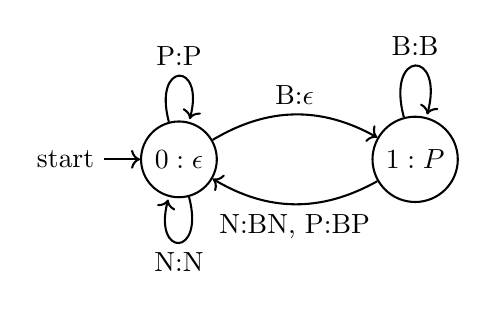
\begin{tikzpicture}
\node[state, initial]  at (0,0) (e) {$0:\epsilon$};
\node[state] at (3,0) (b) {$1:P$};
\path[->] (e) edge[loop above] node{P:P} (e)
		  (e) edge[loop below] node{N:N} (e)
		  (e) edge[above, bend left] node{B:$\epsilon$} (b)
		  (b) edge[below, bend left] node{N:BN, P:BP} (e)
		  (b) edge[loop above] node{B:B} (b);
\end{tikzpicture}
\caption{Subsequential FST for word-final devoicing.}
\label{ssqwfdddd}
\end{figure}

Consider how the transducer in Figure \ref{ssqwfdddd} rewrites the Russian word \emph{pedagog} `pedagogue'.
This word corresponds to the sequence  \emph{PNBNBNB} according to the simplified representation outlined above.
The FST reads symbols of that sequence one by one starting from the initial state $q_0$.
At first, it reads $P$ and $N$ and outputs the same symbols.
The following $B$ leads to the state $q_{1}$, and that $B$ is written together with the following $N$ when the machine moves back to the state $q_0$.
It was delaying the output of $B$ to make sure that only the word-final $B$ is rewritten as $P$.
Finally, when the FST reads the final $B$, it outputs $P$ instead by the state output of $q_{1}$, because it is the final activated state.
The translation of \emph{PNBNBNB} is \emph{PNBNBNP}, that corresponds to correctly rewriting \emph{pedagog} as \emph{pedago[k]} since \emph{[k]} is the voiceless counterpart of \emph{[g]}.


\cite{Chandlee2014}, and later \cite{ChandleeHeinz2018} show that the majority of phonological processes can be modeled in similar ways.
\cite{Chandlee2017} later extends these results to morphology and models different types of affixation, word boundary processes and some types of reduplication.
Other patterns that are shown to be subregular include metathesis, epenthesis, flapping, deletion, harmonies, and many others \citep{Chandlee2014}.
Even some suprasegmental processes, such as stress, seem to exhibit subregular properties \citep{RogersPres}.
For a survey of vowel harmonies and their computational complexities, see \citep{GainorLai12}.
However, some processes, such as reduplication, are not subregular \citep{DolatianHeinz2018}.


The limitations imposed by subregular models provide insights into typology and cognition.
They allow to detect and explain typological gaps, such as the absence of first-last and sour grapes harmonic patterns%
\footnote{The first-last vowel harmony enforces the agreement of the first and the last vowels within a word, and the sour grapes harmony spreads a harmonizing feature only if a blocker is not present \citep{Heinz-Lai-2013-VHS}.}
 \citep{Heinz-Lai-2013-VHS,Luo2017}, and give insights into human cognitive system \citep{RogersPullum2011,Lai15,Avcu2018}.


Although subsequential mappings fit a large portion of natural language patterns, there are phonological processes that are not subsequential.
For example, bidirectional feature spreadings cannot be captured by a subsequential machine because the latter ones can read a string either left-to-right or right-to-left: it cannot pass the value in \emph{both} directions.
Even though this pattern intuitively seems to be pretty simple, two runs of a transducer are required to capture it \citep{Heinz-Lai-2013-VHS}.
As another example, a transducer applying the rules of UTP to the underlying tonal representations is not subsequential either (see Sections \ref{SPldrestrictions} and 4.1.3): for a sequence of low tones to become high, it needs triggers on both sides.
Such mappings are still regular, namely, weakly deterministic and circumambient \citep{Heinz-Lai-2013-VHS,Jardine2016,LamontEtAl2019}.
However, I will focus on a class of subsequential mapping since it subsumes a large portion of attested phonological processes.





\subsection{Left and right subsequential mappings}


Subsequential transducers are a good fit for local and long-distance phonological processes such as intervocalic voicing, word-final devoicing, assimilations, harmonies, and many others.
In all the examples discussed so far (Buryat vowel harmony in Section \ref{FSTforburyat} and Russian word-final devoicing in Section \ref{RussianWFDFST}), the transducer reads the underlying representation left-to-right, correctly capturing the progressive feature spreading.
Such transducers are \textbf{left subsequential}, in contrast to \textbf{right subsequential} FSTs that read the input string right-to-left.

Whereas a left subsequential transducer captures progressive harmonies, it fails to generalize regressive ones.
In the latter, the \emph{last} harmonizing segment contains the information about the feature value that needs to be spread.
For example, in Tuareg, sibilants regressively assimilate in voicing and anteriority; see Section \ref{russianwfdpatternn} for details.
The data below repeats the SFs presented in (7-11), together with the URs, where /S/ represents the underspecified sibilant.

\medskip
\begin{tabular}{llcll}
(39) & \textbf{S}-\textschwa lm\textschwa d & $\rightarrow$ & s-\textschwa lm\textschwa d & `\textsc{caus}-learn' \\
(40) & \textbf{S}-\textschwa q:us\textschwa & $\rightarrow$ & s-\textschwa q:us\textschwa t & `\textsc{caus}-inherit' \\
(41) & \textbf{S}-\textschwa nt\textschwa z & $\rightarrow$ & z-\textschwa nt\textschwa z & `\textsc{caus}-extract' \\
(42) & \textbf{S}-\textschwa m:\textschwa\textesh\textschwa n & $\rightarrow$ & \textesh-\textschwa m:\textschwa\textesh\textschwa n & `\textsc{caus}-be.overwhelmed' \\
(43) & \textbf{S}-\textschwa k:u\textyogh\textschwa t & $\rightarrow$ & \textyogh-\textschwa k:u\textyogh\textschwa t & `\textsc{caus}-saw'
\end{tabular}
\medskip

The right subsequential FST in Figure \ref{ksgjkjgsk} implements the regressive Tuareg sibilant harmony.
For simplicity, $N$ refers to any segment that is not a sibilant.
Every state has a loop reading $N$ and writing the same $N$, therefore non-sibilants are not affected by the harmony in any way.
Additionally, the loop on the state $q_0$ rewrites $S$ as $s$, because an underspecified sibilant is realized as /s/ if there is no other sibilant to its right.
For example, in (39), there is no sibilant in the root, and therefore the causative prefix is realized as /s/.
In other cases (40-43), /S/ agrees with the root sibilant in voicing and anteriority.
For example, in (43), the third segment from the end is \textyogh~ that moves the FST to the state $q_4$, and all following underspecified sibilants are rewritten as \textyogh.



\begin{figure}[h!] 
\centering
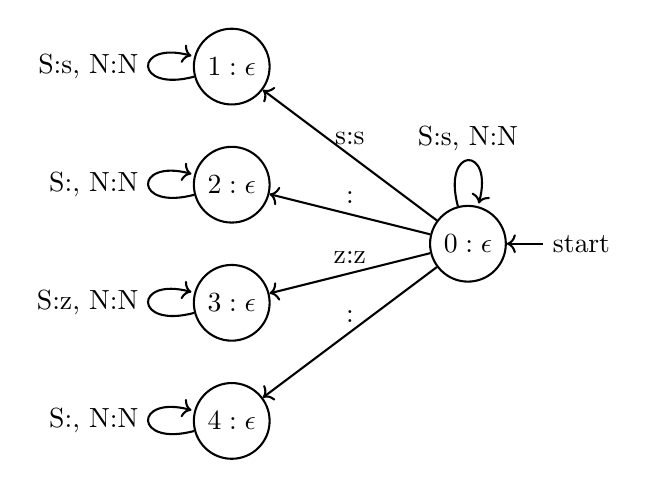
\begin{tikzpicture}
\node[state, initial right]  at (3,0) (e) {$0:\epsilon$};
\node[state] at (0,2.25) (s) {$1:\epsilon$};
\node[state] at (0,0.75) (S) {$2:\epsilon$};
\node[state] at (0,-0.75) (z) {$3:\epsilon$};
\node[state] at (0,-2.25) (Z) {$4:\epsilon$};
\path[->] (e) edge[loop above] node{S:s, N:N} (e)
		  (s) edge[loop left] node{S:s, N:N} (s)
		  (z) edge[loop left] node{S:z, N:N} (z)
		  (S) edge[loop left] node{S:\textesh, N:N} (S)
		  (Z) edge[loop left] node{S:\textyogh, N:N} (Z)
		  (e) edge[above] node{s:s} (s)
		  (e) edge[above] node{\textesh:\textesh} (S)
		  (e) edge[above] node{z:z} (z)
		  (e) edge[above] node{\textyogh:\textyogh} (Z);
\end{tikzpicture}
\caption{Right subsequential FST for Tuareg regressive sibilant harmony.}
\label{ksgjkjgsk}
\end{figure}







\subsection{ISL and OSL mappings}

In this section, I look at two different ways transformational rules can be applied to the underlying representations.
Thus, instead of discussing linguistic patterns, I focus on the \emph{manner of the rule application}.
For instance, consider an SPE-style rule $a \rightarrow b / a~ \_~ a$ from \citep{Chandlee2014}.
There are two ways it can be applied.
Given the UR \emph{aaaaa}, the simultaneous application of this rule to all positions yields the SF \emph{abbba}.
However, if this rule was applied step-by-step, the obtained SF would be \emph{ababa}, since the change of the second $a$ to $b$ makes the context of the third $a$ incompatible with the one specified by the transformation.
To reflect this difference, \cite{Chandlee2014} introduces smaller subclasses of subsequential mappings: \emph{input strictly local} (ISL) and \emph{output strictly local} (OSL) ones.
The ISL functions encode simultaneous rule application of strictly local functions, while the OSL ones reflect the iterative one.
Figure \ref{fig:ssqfunctionsmanyy} shows the relationship among left/right subsequential, ISL and OSL functions.


\begin{figure}[h!]
\begin{center}
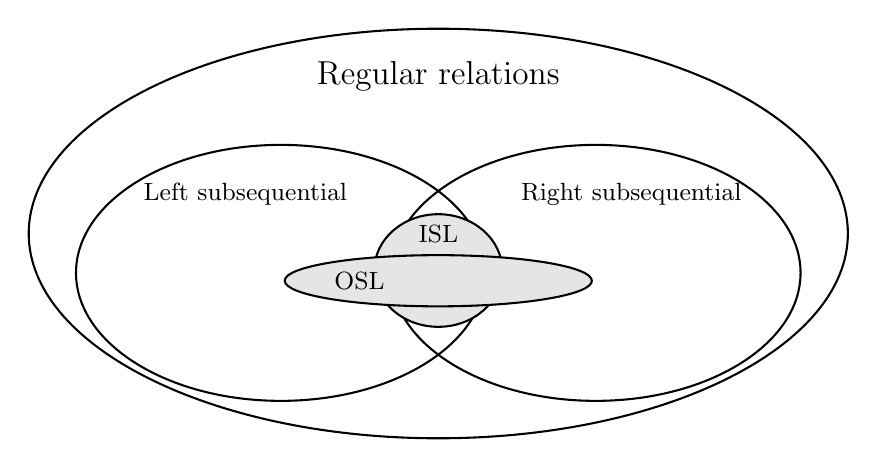
\begin{tikzpicture}
\small    
	\draw (0,0) ellipse (16em and 8em);
    \node at (0,2) {\large Regular relations};
    %
    \draw (-2,-0.5) ellipse (8em and 5em);
    \node at (-2.45,0.5) {Left subsequential};
    %
    \draw (2,-0.5) ellipse (8em and 5em);
    \node at (2.45,0.5) {Right subsequential};
    %
    \draw[black,fill=gray!20] (0, -0.47) ellipse (2.5em and 2.2em);
    \node at (0,0) {ISL};
    %
    \draw[black,fill=gray!20] (0, -0.6) ellipse (6em and 1em);
    \node at (-1,-0.6) {OSL};
\end{tikzpicture}
\caption{Relationship among left subsequential, right subsequential, OSL, and ISL functions; adapted from \citep{Chandlee2014}.}
\label{fig:ssqfunctionsmanyy}
\end{center}
\end{figure}





\cite{ChandleeEtAl2014} define both ISL and OSL mappings using the notion of \textbf{tails}.
Tails show the dependency between the possible continuations of input strings, and portions of the output contributed by those continuations.
Formally, tails are defined as $tails(x) = \{(y, v) : f(x\cdot y) = u\cdot v \textrm{ and } u = lcp(f(x\cdot \Sigma^*))\}$, where $f$ is the function mapping the input strings to the corresponding outputs, $\cdot$ is the concatenation operator, and $lcp$ is the longest common prefix.
For example, the longest common prefix of $abc$ and $abde$ is $ab$, since it is the longest prefix shared by those two strings.
A slightly extended notation introduced below changes that definition to $tails(\vv{\bm{x}}) = \{(y, v) : f(\vv{\bm{x}}\cdot y) = \bm{u}\cdot v \textrm{ and } u = lcp(f(\vv{\bm{x}}\cdot \Sigma^*))\}$.



Assume that $\Sigma$ and $\Gamma$ are (possibly different) alphabets used to represent the strings before and after application of some rule.
Additionally, strings $\vv{\bm{x}}$ and $y$ belong to $\Sigma^*$, and $\bm{u}$ and $v$ belong to $\Gamma^*$, i.e.\ these strings consist only of symbols included in $\Sigma^*$ or $\Gamma^*$, respectively.
A tail of the prefix $\vv{\bm{x}}$ is a list of all pairs $(y, v)$, where $y$ is a possible continuation of the input prefix $\vv{\bm{x}}$, i.e.\ $\vv{\bm{x}}\cdot y$ is the input string.
The corresponding to $\vv{\bm{x}}\cdot y$ output string is $\bm{u}\cdot v$, where $\bm{u}$ is the longest prefix shared by all outputs corresponding to inputs starting with $\vv{\bm{x}}$.


As an example, let us find a list of tails of the input prefix $\vv{\bm{\bow aa}}$ in the mapping $M$.
Note, that only the input strings are annotated with the edges $\bow$ and $\eow$.


\begin{multline*}
M = (\bow aa\eow, aa), (\bow aaa\eow, aba), (\bow aaaa\eow, abba), (\bow aaaaa\eow, abbba), \\
 \qquad\quad \shoveleft{(\bow aaaaaa\eow, abbbba), (\bow aaaaaaa\eow, abbbbba)\dots}
\end{multline*}


All input strings of that mapping start with $\vv{\bm{\bow aa}}$.
The longest common prefix of the corresponding output strings is $\bm{a}$: for example, the second symbol is different in $aa$ and $aba$.
Below, I mark the selected input prefix $\vv{\bm{\bow aa}}$ and the longest common prefix $\bm{a}$.


$$
M_{marked} = (\vv{\bm{\bow aa}}\eow, \bm{a}a), (\vv{\bm{\bow aa}}a\eow, \bm{a}ba), (\vv{\bm{\bow aa}}aa\eow, \bm{a}bba), (\vv{\bm{\bow aa}}aaa\eow, \bm{a}bbba) \dots
$$

The list of tails of $\vv{\bm{\bow aa}}$ can be computed by removing $\vv{\bm{\bow aa}}$ and $\bm{a}$ from the input and output strings of $M_{marked}$, respectively.

$$
tails(\vv{\bm{\bow aa}}) = (\eow, a), (a\eow, ba), (aa\eow, bba), (aaa\eow, bbba)\dots
$$

The obtained list of tails implies that after observing $\vv{\bm{\bow aa}}$, the input continuation $\eow$ introduces $a$ to the translation,  $a\eow$ contributes $ba$, and so on.
Further in this subsection, I show how the notion of tails is used to define ISL and OSL mappings \citep{Chandlee2014,ChandleeEtAl2014,ChandleeEtAl2015}.



\subsubsection{Input strictly local mappings}

The $k$-ISL functions encode simultaneous rule application, i.e.\ when a transformational rule applied to all positions at the same time.
In mapping $M$, for example, $a$ is substituted by $b$ if it is surrounded by $a$ \emph{in the input string}.
It creates pairs such as $(aaaaa, abbba)$: three internal $a$ 
are changed to $b$ since their context in the input string is the same as specified by the rule $a \rightarrow b / a~ \_~ a$.

\cite{ChandleeEtAl2014} define an ISL mapping as follows.
If two input strings $u_1$ and $u_2$ share the same $k-1$-local suffix, their set of tails is identical as well.

\[
	\textrm{\emph{suff}}^{k-1}(u_1) = \textrm{\emph{suff}}^{k-1}(u_2) \Rightarrow~ tails(u_1) = tails(u_2)
\]

If the mapping $M$ is indeed ISL, the set of tails is the same for all strings ending with the same $k-1$ local prefix.
Let us assume that $k=3$, since the rule targets an item in the context of two other elements.
Input strings $\bow aa\eow$ and $\bow aaa\eow$ both have the $2$-local suffix $a\eow$, and that definition states that their sets of tails must be identical as well.
To confirm this, let us compare tails of $\bow aa$ and $\bow aaa$.


\begin{multline*}
tails(\vv{\bm{\bow aa}}) = (\vv{\bm{\bow aa}}\eow, \bm{a}a), (\vv{\bm{\bow aa}}a\eow, \bm{a}ba), (\vv{\bm{\bow aa}}aa\eow, \bm{a}bba) \dots~ =  \\
 \qquad\qquad\qquad\qquad\quad \shoveleft{(\eow, a), (a\eow, ba), (aa\eow, bba) \dots}
\end{multline*}

\begin{multline*}
tails(\vv{\bm{\bow aaa}}) = (\vv{\bm{\bow aaa}}\eow, \bm{ab}a), (\vv{\bm{\bow aaa}}a\eow, \bm{ab}ba), (\vv{\bm{\bow aaa}}aa\eow, \bm{ab}bba) \dots~ =  \\
 \qquad\qquad\qquad\qquad\quad \shoveleft{(\eow, a), (a\eow, ba), (aa\eow, bba) \dots}
\end{multline*}

Their tails are indeed the same, and it confirms that the \emph{simultaneous application} of the rule $a \rightarrow b / a~ \_~ a$ is an \emph{ISL} function.
The corresponding transducer encodes a $3$-local window reading the input string.
Knowledge of the previous $2$ input symbols informs the transducer about the next action regarding the following symbol that it reads.
Figure \ref{fig:fwoeirwj} demonstrates these steps.

\begin{figure}[h!]
\begin{center}
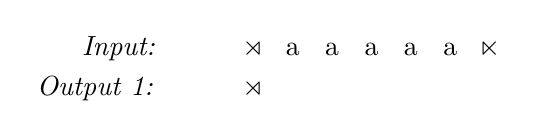
\begin{tikzpicture}
\node at (-1.7,0.25) {\emph{Input:}};
\node (0) at (0,0.25) {$\rtimes$};
\node (1) at (0.5,0.25) {a};
\node (2) at (1,0.25) {a};
\node (3) at (1.5,0.25) {a};
\node (4) at (2,0.25) {a};
\node (5) at (2.5,0.25) {a};
\node (6) at (3,0.25) {$\ltimes$};
%
\node at (-2,-0.25) {\emph{Output 1:}};
\node (0) at (0,-0.25) {$\rtimes$};
\end{tikzpicture}
\vspace{0.5em}


\begin{tikzpicture}
\node at (-1.7,0.25) {\emph{Input:}};
\node (0) at (0,0.25) {$\rtimes$};
\node (1) at (0.5,0.25) {a};
\node (2) at (1,0.25) {a};
\node (3) at (1.5,0.25) {a};
\node (4) at (2,0.25) {a};
\node (5) at (2.5,0.25) {a};
\node (6) at (3,0.25) {$\ltimes$};
%
\node at (-2,-0.25) {\emph{Output 2:}};
\node (0) at (0,-0.25) {$\rtimes$};
\node (01) at (0.5,-0.25) {a};
%
\draw [dashed] (-0.2,0) -- (-0.2,0.5) -- (1.2,0.5) -- (1.2,0) -- (-0.2,0);
\draw [dashed] (0.25, 0) -- (0.25, 0.5);
\draw [dashed] (0.75, 0) -- (0.75, 0.5);
\end{tikzpicture}
\vspace{0.5em}


\begin{tikzpicture}
\node at (-1.7,0.25) {\emph{Input:}};
\node (0) at (0,0.25) {$\rtimes$};
\node (1) at (0.5,0.25) {a};
\node (2) at (1,0.25) {a};
\node (3) at (1.5,0.25) {a};
\node (4) at (2,0.25) {a};
\node (5) at (2.5,0.25) {a};
\node (6) at (3,0.25) {$\ltimes$};
%
\node at (-2,-0.25) {\emph{Output 3:}};
\node (0) at (0,-0.25) {$\rtimes$};
\node (01) at (0.5,-0.25) {a};
\node (01) at (1,-0.25) {b};
%
\draw [dashed] (-0.2+0.5,0) -- (-0.2+0.5,0.5) -- (1.2+0.5,0.5) -- (1.2+0.5,0) -- (-0.2+0.5,0);
\draw [dashed] (0.25+0.5, 0) -- (0.25+0.5, 0.5);
\draw [dashed] (0.75+0.5, 0) -- (0.75+0.5, 0.5);
\end{tikzpicture}
\vspace{0.5em}

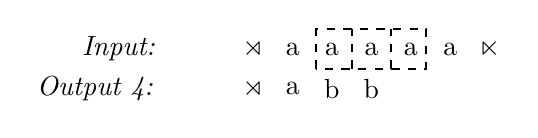
\begin{tikzpicture}
\node at (-1.7,0.25) {\emph{Input:}};
\node (0) at (0,0.25) {$\rtimes$};
\node (1) at (0.5,0.25) {a};
\node (2) at (1,0.25) {a};
\node (3) at (1.5,0.25) {a};
\node (4) at (2,0.25) {a};
\node (5) at (2.5,0.25) {a};
\node (6) at (3,0.25) {$\ltimes$};
%
\node at (-2,-0.25) {\emph{Output 4:}};
\node (0) at (0,-0.25) {$\rtimes$};
\node (01) at (0.5,-0.25) {a};
\node (01) at (1,-0.25) {b};
\node (01) at (1.5,-0.25) {b};
%
\draw [dashed] (-0.2+1,0) -- (-0.2+1,0.5) -- (1.2+1,0.5) -- (1.2+1,0) -- (-0.2+1,0);
\draw [dashed] (0.25+1, 0) -- (0.25+1, 0.5);
\draw [dashed] (0.75+1, 0) -- (0.75+1, 0.5);
\end{tikzpicture}
\vspace{0.5em}

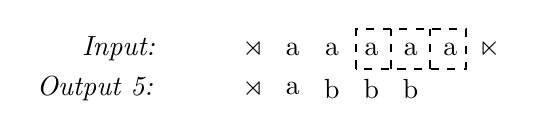
\begin{tikzpicture}
\node at (-1.7,0.25) {\emph{Input:}};
\node (0) at (0,0.25) {$\rtimes$};
\node (1) at (0.5,0.25) {a};
\node (2) at (1,0.25) {a};
\node (3) at (1.5,0.25) {a};
\node (4) at (2,0.25) {a};
\node (5) at (2.5,0.25) {a};
\node (6) at (3,0.25) {$\ltimes$};
%
\node at (-2,-0.25) {\emph{Output 5:}};
\node (0) at (0,-0.25) {$\rtimes$};
\node (01) at (0.5,-0.25) {a};
\node (01) at (1,-0.25) {b};
\node (01) at (1.5,-0.25) {b};
\node (01) at (2,-0.25) {b};
%
\draw [dashed] (-0.2+1.5,0) -- (-0.2+1.5,0.5) -- (1.2+1.5,0.5) -- (1.2+1.5,0) -- (-0.2+1.5,0);
\draw [dashed] (0.25+1.5, 0) -- (0.25+1.5, 0.5);
\draw [dashed] (0.75+1.5, 0) -- (0.75+1.5, 0.5);
\end{tikzpicture}
\vspace{0.5em}

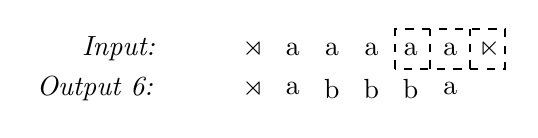
\begin{tikzpicture}
\node at (-1.7,0.25) {\emph{Input:}};
\node (0) at (0,0.25) {$\rtimes$};
\node (1) at (0.5,0.25) {a};
\node (2) at (1,0.25) {a};
\node (3) at (1.5,0.25) {a};
\node (4) at (2,0.25) {a};
\node (5) at (2.5,0.25) {a};
\node (6) at (3,0.25) {$\ltimes$};
%
\node at (-2,-0.25) {\emph{Output 6:}};
\node (0) at (0,-0.25) {$\rtimes$};
\node (01) at (0.5,-0.25) {a};
\node (01) at (1,-0.25) {b};
\node (01) at (1.5,-0.25) {b};
\node (01) at (2,-0.25) {b};
\node (01) at (2.5,-0.25) {a};
%
\draw [dashed] (-0.2+2,0) -- (-0.2+2,0.5) -- (1.2+2,0.5) -- (1.2+2,0) -- (-0.2+2,0);
\draw [dashed] (0.25+2, 0) -- (0.25+2, 0.5);
\draw [dashed] (0.75+2, 0) -- (0.75+2, 0.5);
\end{tikzpicture}
\vspace{0.5em}

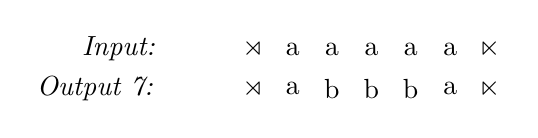
\begin{tikzpicture}
\node at (-1.7,0.25) {\emph{Input:}};
\node (0) at (0,0.25) {$\rtimes$};
\node (1) at (0.5,0.25) {a};
\node (2) at (1,0.25) {a};
\node (3) at (1.5,0.25) {a};
\node (4) at (2,0.25) {a};
\node (5) at (2.5,0.25) {a};
\node (6) at (3,0.25) {$\ltimes$};
%
\node at (-2,-0.25) {\emph{Output 7:}};
\node (0) at (0,-0.25) {$\rtimes$};
\node (01) at (0.5,-0.25) {a};
\node (01) at (1,-0.25) {b};
\node (01) at (1.5,-0.25) {b};
\node (01) at (2,-0.25) {b};
\node (01) at (2.5,-0.25) {a};
\node (6) at (3,-0.25) {$\ltimes$};
\end{tikzpicture}
\caption{ISL application of the rule $a \rightarrow b / a~ \_~ a$ to \emph{aaaaa}.}
\label{fig:fwoeirwj}
\end{center}
\end{figure}

\subsubsection{Output strictly local mappings}

Now, let us consider the iterative application of the same rule $a \rightarrow b / a~ \_~ a$.
In this case, every time the rule is applied, it changes the form that the same rule produced earlier, and therefore $aaaaa$ is changed to $ababa$.
This type of transformation can be visualized as a $3$-local window moving through the input string and rewriting the middle item if the contexts match.
The steps below show the application of the rule; the underlined segments are the contexts, and the boxed items show how the target element was changed.
The list of pairs in $M'$ shows the corresponding mapping.

$$
\underline{\bow}\dbox{a:a}\underline{a}aaa\eow~ \rightarrow
\bow\underline{a}\dbox{a:b}\underline{a}aa\eow~ \rightarrow
\bow a\underline{b}\dbox{a:a}\underline{a}a\eow~ \rightarrow
\bow ab\underline{a}\dbox{a:b}\underline{a}\eow~ \rightarrow
\bow aba\underline{b}\dbox{a:a}\underline{\eow}
$$

\begin{multline*}
M' = (\bow aa\eow, aa), (\bow aaa\eow, aba), (\bow aaaa\eow, abaa), (\bow aaaaa\eow, ababa), \\
 \qquad\quad \shoveleft{(\bow aaaaaa\eow, ababaa), (\bow aaaaaaa\eow, abababa)\dots}
\end{multline*}

\cite{ChandleeEtAl2015} shows that such mappings are $k$-OSL since the previous application of this rule affects the following one.
Their definition of OSL mappings is below, where the function $f$, as previously, maps its argument (input string) to the corresponding output.
For a mapping to be OSL, the following needs to be true: if two output strings share the same $k-1$-local suffix, the tails of the corresponding input strings are the same.


\[
	suff^{k-1}(f(u_1)) = suff^{k-1}(f(u_2)) \Rightarrow~ tails(u_1) = tails(u_2)
\]

That would imply that in the mapping $M'$, tails of $\vv{\bm{\bow aaa}}$ and $\vv{\bm{\bow aaaaa}}$ are the same because the translations of $\bow aaa\eow$ and $\bow aaaaa\eow$ share the same $k-1$-local suffix $ba$ (those translations are $aba$ and $ababa$, respectively).

\begin{multline*}
tails(\vv{\bm{\bow aaa}}) = (\vv{\bm{\bow aaa}}\eow, \bm{aba}), (\vv{\bm{\bow aaa}}a\eow, \bm{aba}a), (\vv{\bm{\bow aaa}}aa\eow, \bm{aba}ba) \dots~ =  \\
 \qquad\qquad\qquad\qquad\quad \shoveleft{(\eow, \epsilon), (a\eow, a), (aa\eow, ba) \dots}
\end{multline*}

\begin{multline*}
tails(\vv{\bm{\bow aaaaa}}) = \\
\qquad \shoveleft{(\vv{\bm{\bow aaaaa}}\eow, \bm{ababa}), (\vv{\bm{\bow aaaaa}}a\eow, \bm{ababa}a), (\vv{\bm{\bow aaaaa}}aa\eow, \bm{ababa}ba) \dots~ =}  \\
 \qquad\qquad\qquad\qquad\quad \shoveleft{(\eow, \epsilon), (a\eow, a), (aa\eow, ba) \dots}
\end{multline*}

Indeed, since their tails are the same, this shows that the mapping is OSL.
The corresponding transducer encodes a $3$-local window that keeps track of the last $2$ output symbols.
Based on those symbols and the current symbol it decides how that current symbol is changed.
The iterative rule application is demonstrated in Figure \ref{fig:dgsldkgjsd}.



\begin{figure}[t]
\begin{center}
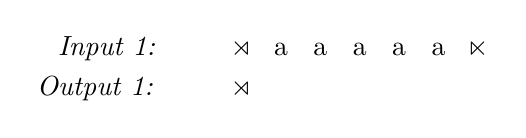
\begin{tikzpicture}
\node at (-1.7,0.25) {\emph{Input 1:}};
\node (0) at (0,0.25) {$\rtimes$};
\node (1) at (0.5,0.25) {a};
\node (2) at (1,0.25) {a};
\node (3) at (1.5,0.25) {a};
\node (4) at (2,0.25) {a};
\node (5) at (2.5,0.25) {a};
\node (6) at (3,0.25) {$\ltimes$};
%
\node at (-1.85,-0.25) {\emph{Output 1:}};
\node (0) at (0,-0.25) {$\rtimes$};
\end{tikzpicture}
\vspace{0.5em}


\begin{tikzpicture}
\node at (-1.7,0.25) {\emph{Input 2:}};
\node (0) at (0,0.25) {$\rtimes$};
\node (1) at (0.5,0.25) {a};
\node (2) at (1,0.25) {a};
\node (3) at (1.5,0.25) {a};
\node (4) at (2,0.25) {a};
\node (5) at (2.5,0.25) {a};
\node (6) at (3,0.25) {$\ltimes$};
%
\node at (-1.85,-0.25) {\emph{Output 2:}};
\node (0) at (0,-0.25) {$\rtimes$};
\node (01) at (0.5,-0.25) {a};
%
\draw [dashed] (0.25,0) -- (0.25,0.5) -- (1.2,0.5) -- (1.2,0) -- (0.25,0);
\draw [dashed] (-0.2, 0) -- (0.25, 0) -- (0.25, -0.5) -- (-0.2, -0.5) -- (-0.2, 0);
\draw [dashed] (0.75, 0) -- (0.75, 0.5);
\end{tikzpicture}
\vspace{0.5em}

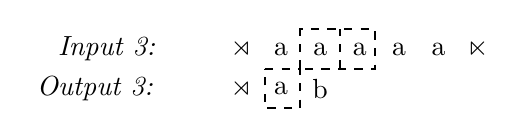
\begin{tikzpicture}
\node at (-1.7,0.25) {\emph{Input 3:}};
\node (0) at (0,0.25) {$\rtimes$};
\node (1) at (0.5,0.25) {a};
\node (2) at (1,0.25) {a};
\node (3) at (1.5,0.25) {a};
\node (4) at (2,0.25) {a};
\node (5) at (2.5,0.25) {a};
\node (6) at (3,0.25) {$\ltimes$};
%
\node at (-1.85,-0.25) {\emph{Output 3:}};
\node (0) at (0,-0.25) {$\rtimes$};
\node (01) at (0.5,-0.25) {a};
\node (01) at (1,-0.25) {b};
%
\draw [dashed] (0.25 + 0.5,0) -- (0.25 + 0.5,0.5) -- (1.2 + 0.5,0.5) -- (1.2 + 0.5,0) -- (0.25 + 0.5,0);
\draw [dashed] (-0.2 + 0.5, 0) -- (0.25 + 0.5, 0) -- (0.25 + 0.5, -0.5) -- (-0.2 + 0.5, -0.5) -- (-0.2 + 0.5, 0);
\draw [dashed] (0.75 + 0.5, 0) -- (0.75 + 0.5, 0.5);
\end{tikzpicture}
\vspace{0.5em}

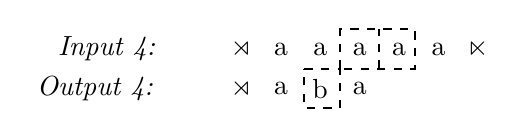
\begin{tikzpicture}
\node at (-1.7,0.25) {\emph{Input 4:}};
\node (0) at (0,0.25) {$\rtimes$};
\node (1) at (0.5,0.25) {a};
\node (2) at (1,0.25) {a};
\node (3) at (1.5,0.25) {a};
\node (4) at (2,0.25) {a};
\node (5) at (2.5,0.25) {a};
\node (6) at (3,0.25) {$\ltimes$};
%
\node at (-1.85,-0.25) {\emph{Output 4:}};
\node (0) at (0,-0.25) {$\rtimes$};
\node (01) at (0.5,-0.25) {a};
\node (01) at (1,-0.25) {b};
\node (01) at (1.5,-0.25) {a};
%
\draw [dashed] (0.25 + 1,0) -- (0.25 + 1,0.5) -- (1.2 + 1,0.5) -- (1.2 + 1,0) -- (0.25 + 1,0);
\draw [dashed] (-0.2 + 1, 0) -- (0.25 + 1, 0) -- (0.25 + 1, -0.5) -- (-0.2 + 1, -0.5) -- (-0.2 + 1, 0);
\draw [dashed] (0.75 + 1, 0) -- (0.75 + 1, 0.5);
\end{tikzpicture}
\vspace{0.5em}

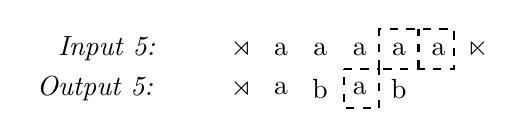
\begin{tikzpicture}
\node at (-1.7,0.25) {\emph{Input 5:}};
\node (0) at (0,0.25) {$\rtimes$};
\node (1) at (0.5,0.25) {a};
\node (2) at (1,0.25) {a};
\node (3) at (1.5,0.25) {a};
\node (4) at (2,0.25) {a};
\node (5) at (2.5,0.25) {a};
\node (6) at (3,0.25) {$\ltimes$};
%
\node at (-1.85,-0.25) {\emph{Output 5:}};
\node (0) at (0,-0.25) {$\rtimes$};
\node (01) at (0.5,-0.25) {a};
\node (01) at (1,-0.25) {b};
\node (01) at (1.5,-0.25) {a};
\node (01) at (2,-0.25) {b};
%
\draw [dashed] (0.25 + 1.5,0) -- (0.25 + 1.5,0.5) -- (1.2 + 1.5,0.5) -- (1.2 + 1.5,0) -- (0.25 + 1.5,0);
\draw [dashed] (-0.2 + 1.5, 0) -- (0.25 + 1.5, 0) -- (0.25 + 1.5, -0.5) -- (-0.2 + 1.5, -0.5) -- (-0.2 + 1.5, 0);
\draw [dashed] (0.75 + 1.5, 0) -- (0.75 + 1.5, 0.5);
\end{tikzpicture}
\vspace{0.5em}

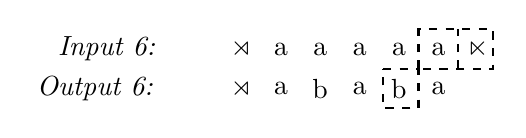
\begin{tikzpicture}
\node at (-1.7,0.25) {\emph{Input 6:}};
\node (0) at (0,0.25) {$\rtimes$};
\node (1) at (0.5,0.25) {a};
\node (2) at (1,0.25) {a};
\node (3) at (1.5,0.25) {a};
\node (4) at (2,0.25) {a};
\node (5) at (2.5,0.25) {a};
\node (6) at (3,0.25) {$\ltimes$};
%
\node at (-1.85,-0.25) {\emph{Output 6:}};
\node (0) at (0,-0.25) {$\rtimes$};
\node (01) at (0.5,-0.25) {a};
\node (01) at (1,-0.25) {b};
\node (01) at (1.5,-0.25) {a};
\node (01) at (2,-0.25) {b};
\node (01) at (2.5,-0.25) {a};
%
\draw [dashed] (0.25 + 2,0) -- (0.25 + 2,0.5) -- (1.2 + 2,0.5) -- (1.2 + 2,0) -- (0.25 + 2,0);
\draw [dashed] (-0.2 + 2, 0) -- (0.25 + 2, 0) -- (0.25 + 2, -0.5) -- (-0.2 + 2, -0.5) -- (-0.2 + 2, 0);
\draw [dashed] (0.75 + 2, 0) -- (0.75 + 2, 0.5);
\end{tikzpicture}
\vspace{0.5em}

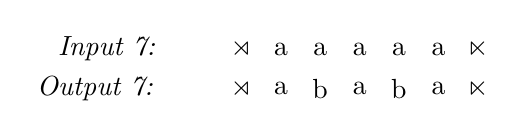
\begin{tikzpicture}
\node at (-1.7,0.25) {\emph{Input 7:}};
\node (0) at (0,0.25) {$\rtimes$};
\node (1) at (0.5,0.25) {a};
\node (2) at (1,0.25) {a};
\node (3) at (1.5,0.25) {a};
\node (4) at (2,0.25) {a};
\node (5) at (2.5,0.25) {a};
\node (6) at (3,0.25) {$\ltimes$};
%
\node at (-1.85,-0.25) {\emph{Output 7:}};
\node (0) at (0,-0.25) {$\rtimes$};
\node (01) at (0.5,-0.25) {a};
\node (01) at (1,-0.25) {b};
\node (01) at (1.5,-0.25) {a};
\node (01) at (2,-0.25) {b};
\node (01) at (2.5,-0.25) {a};
\node (6) at (3,-0.25) {$\ltimes$};
\end{tikzpicture}

\caption{OSL application of the rule $a \rightarrow b / a~ \_~ a$ to \emph{aaaaa}.}
\label{fig:dgsldkgjsd}
\end{center}
\end{figure}




To sum up, $k$-ISL and $k$-OSL mappings encode dependencies affecting $k$-local windows.
ISL functions apply a rule simultaneously to all the positions of the input string, whereas the OSL functions apply a rule step-by-step.
While in the former case, the changes are independent from each other, the latter uses information about the previous change to inform the following one.
\cite{Chandlee2014} argues that linguistic strictly local processes are ISL or OSL, and demonstrates it using a variety of linguistic examples such as Greek fricative deletion, English flapping, and others \citep{JosephPhilippakiWarburton1987}.




\subsection{Models of transformations: summary}


FSTs encode regular mappings that are well-known to be a good fit for natural language phonology and morphology \citep{Johnson1972,KaplanKay94,BeesleyKartunnen03}.
However, a particular class of functions, namely, \emph{subsequential}, includes the major part of natural language patterns.
Transducers implementing subsequential mappings read the symbols of the underlying representations one by one and output the corresponding surface forms.
This allows one to model local and long-distance processes, such as word-final devoicing and vowel harmony.

It should be noted that some attested phonological processes are not subsequential.
Among them, there are circumambient pattern of unbounded tonal plateauing and reduplication requiring the power of two-way FSTs \citep{Jardine2016,DolatianHeinz2018}.
Those patterns, however, are beyond the scope of this dissertation.


In Chapter 4, I discuss results of tool-assisted learning experiments targeting various phonological processes such as tone plateauing, local processes, and different types of harmony systems with and without blockers.





\section{Learning grammars from data}
\label{learningframework}


Previous sections showed that subregular grammars can model natural language dependencies.
However, all the previously presented grammars were constructed manually.
In this section, I discuss the possibility of building those models \emph{automatically}.
It not only allows the researchers to avoid the burden of manual grammar construction, but also gives us insights into the mechanisms helping to discover those patters.


\emph{Grammatical inference} is a sub-field of machine learning 
that is concerned with the extraction of grammars from data.
As Colin de la Higuera formulates in his book ``Grammatical Inference'' (\citeyear{DeLaHiguera2010}), this field lies at the intersection of linguistics, inductive analysis, and pattern recognition.
\emph{Linguistics}, and computational linguistics, in particular, brings the core idea of the existence of a \emph{formal grammar}, or a set of rules defining a \emph{language}.
\emph{Language learning} can then be viewed as a process of discovering a language's grammar by the learner.
The field of \emph{inductive inference} aims at a problem of inferring the underlying grammar that consistently predicts what is grammatical and what is not after observing a set of elements of the language, where those elements can be strings, trees, or other structured objects.
Finally, \emph{pattern recognition} describes the best model and its properties that would explain the data; it \emph{analyzes} the pattern.

If the task is to model a language, then the goal is to find a grammar that describes that language.
If the grammar is not known a priori, it might be possible to \emph{learn} its rules by observing and exploring the language.
\emph{Grammatical inference algorithms} require a finite sample of usually positive data drawn from the target language as input, and return a grammar hypothesis as output.
That grammar solves a \emph{membership problem} for that language, or, in other words, it correctly predicts for any given string if that string belongs to the target language, see Figure \ref{fig:LGrel}.
If instead a mapping needs to be learned, grammatical inference algorithms require a sufficient sample of the input-output pairs as input and construct a transducer that generalizes that mapping.

\begin{figure}[t]
  \centering
  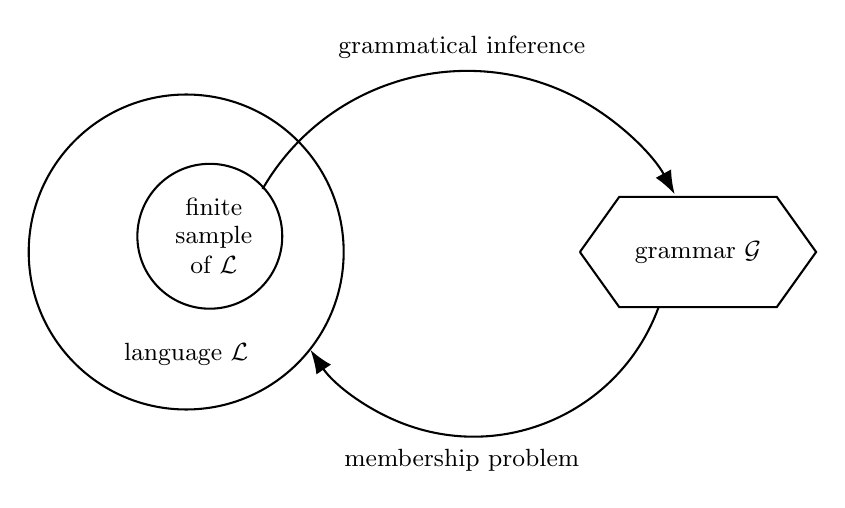
\begin{tikzpicture}
  \small
    \draw (0.3,0.2) circle (0.92cm);
    \draw (0,0) circle (2cm);
    \draw (5,0) -- (5.5,0.7) -- (7.5,0.7) -- (8,0) -- (7.5,-0.7) -- (5.5,-0.7) -- (5,0);
    \draw[-{Latex[length=3mm]}] (0.97,0.8) arc (150:28.5:3cm);
    \draw[-{Latex[length=3mm]}] (6,-0.7) arc (-20:-146:2.5cm);
    
    \path (0.35,0.2) node[text width=1.5cm,align=center] {\baselineskip=10pt finite sample \\ of $\mathcal{L}$};
    \path (0, -1.3) node[text width=2cm,align=center] {\baselineskip=10pt language $\mathcal{L}$};
    \path (6.5, 0) node[text width=2cm,align=center] {\baselineskip=10pt grammar $\mathcal{G}$};
    \path (3.5, 2.6) node[text width=4cm,align=center] {\baselineskip=10pt grammatical inference};
     \path (3.5,-2.65) node[text width=4cm,align=center] {\baselineskip=10pt membership problem};
  \end{tikzpicture}
  \caption{Relationship between a language $\mathcal{L}$ and a grammar $\mathcal{G}$.}
  \label{fig:LGrel}
\end{figure}


The learning algorithms for SL, SP, TSL and MTSL languages, and also the algorithm inferring subsequential mappings, will be discussed in details in Chapters 3 and 4.
These algorithms share several common properties, namely, they all require only positive data to find the grammar, they are fully interpretable, and work in polynomial time and data.
Indeed, \emph{learning only from the positive data} is the desired characteristic, since human learners do not have access to what is not possible in their languages \citep{Chomsky1986}.
Only some of the subregular languages have this property: the full class of regular languages cannot be learned from positive data.
\emph{Interpretability} of an algorithm means that both the learning process and the outcome are transparent: it is possible to trace how the learner came to a certain conclusion, and explain the obtained results.
These learners extract grammars in \emph{polynomial time}, so they can be computed in practice.
(The running time of polynomial algorithms is $n^c$, where $n$ is the size of the training sample, and $c$ is some constant \citep{Sipser2013}.)
Finally, \emph{learning in the limit} guarantees that after a finite number of errors, the learner will start making only correct predictions \citep{Gold1967}. 

As a part of my dissertation, I implemented the \emph{SigmaPie} package \href{https://pypi.org/project/SigmaPie/}{\faCube} for working with subregular languages and mappings.
It provides learners for SL, TSL, MTSL, SP languages and subsequential mappings \citep{sigmapie}.
In Chapter 3, I explore how well those subregular learners extract \emph{well-formedness conditions} from artificial automatically generated datasets exhibiting human language-like patterns such as one or more harmonies with or without blockers, word-final devoicing, tone plateauing, and others.
The training sample for those experiments is a collection of words well-formed according to one of those generalizations.
Later in Chapter 4, I explore modeling of \emph{processes} similar to the ones listed above.
In this case, the training sample contains pairs of underlying representations and the corresponding surface forms.
In such a way, I model processes and well-formedness conditions using tools implemented as a part of \emph{SigmaPie}.


\section{Aspects of practical applications}
\label{aspects}


There were several successful applications of grammatical inference algorithms in the previous decades.
For example, Alexander Clark won the Tenjinno competition in 2006 by using a modified version of OSTIA, a subsequential learner discussed further in Chapter 4 \citep{OncinaEtAl1993,Clark2006}.
Also, \cite{Chandlee-FuEtAl-2012-IGIRP} explore the integration of FSA-based grammatical inference techniques into robotic planning.


However, the subregular learners are \emph{structural} and not probabilistic, and therefore frequently, the absence of some particular configuration in the training sample results in the algorithm failing to learn simple patterns.
For instance, \cite{GildeaJurafsky1996} show that a corpus of English pronunciations is not enough for OSTIA to generalize a rule of English flapping.


Indeed, the results of my Chapters 3 and 4 confirm that local restrictions and gaps in the natural language data obscure the extraction of some dependencies.
This is why I mostly focused on learning \emph{sub-phenomena} instead of the complex interactions of local and long-distance dependencies found in natural language data.
Alternatively, capturing different aspects of the data can be done by combining forces of different learners \citep{Heinz10ldp,HeinzIdsardi13}.


There are other directions of research that could improve the performance of subregular learners.
For example, implementing linguistic notions such as features can help to see the behavior of elements as groups instead of individual segments.
The initial results on integrating features and natural classes are available in \citep{Strother-Garcia-HeinzEtAl-2016-UMTGICSP,chandlee-etal-2019-learning}.
Some prior knowledge about the shape of the data can be encoded into the learners using methods that help to systematically exclude certain possible configurations from consideration, as it was shown by \cite{WellmanHenrion1993}.
Also, adding probabilities to the learning algorithms allows abandoning the ``black and white'' structural approach incapable of modeling such probabilistic phenomena as harmony fading or the occurrence of disharmonic words.
\cite{HeinzRogers2010SPdist,Shibata-Heinz-2019-MLEFRDSL} explore the probabilistic subregular models, and \cite{Heinz-Koirala-2010-MLEFD,VuZehfrooshEtal2018-SRLUSM} add together features and probabilities.



%\setcounter{chapter}{2}
\chapter{Learning languages}
\label{languageschapter}
In the previous chapter, I showed that different phonological and morphological phenomena can be modeled as subregular languages.
Indeed, local processes can be expressed with strictly local (SL) grammars and long-distance processes with strictly piecewise (SP) grammars.
If a long-distance process uses blockers (e.g., opaque vowels in vowel harmony), then we use tier-based strictly local (TSL) grammars.
If the language shows multiple long-distance processes, then we may also need  multi-tier strictly local (MTSL) grammars.
This perspective on morphotactics and phonotactics also rules out typologically unattested patterns such as first-last harmony, majority harmony, or embedded circumfixation.

In this chapter, I discuss algorithms which extract SL, SP, TSL and MTSL grammars from the data.
Apart from the training sample, these algorithms require knowing the class of the target grammar, and the locality window of that grammar, i.e.\ the length of substructures with which it operates.
In other words, we need to know the formal complexity of the target language in order to learn it efficiently using subregular learning algorithms.
Given a sufficient and representative training sample and proper specifications of the target grammar, the subregular learners discover the pattern in polynomial time and data.

I start by introducing the datasets that I will use throughout the chapter to perform the learning experiments.
These datasets vary from automatically generated artificial languages to real wordlists exemplifying concrete linguistic phenomena, such as word-final devoicing in German, vowel harmony in Turkish, and others.
I then use these datasets as training samples for the subregular learners, discuss the obtained grammars, and automatically evaluate the predictions of those grammars based on the well-formedness of the strings they generate.
At the end of the chapter, I provide a table that summarizes the results of the learning experiments.

The exemplified learners work exclusively with \emph{string representations}.
These algorithms focus on structural properties; they are limited to non-probabilistic algorithms which evaluate the well-formedness of input strings.
As of now, I have not implemented statistical versions of these algorithms, or algorithms which work with non-string-based representations.


The subregular learners, scanners and sample generators are available as a module of my Python package \emph{SigmaPie} \href{https://pypi.org/project/SigmaPie/}{\faCube} \citep{sigmapie}.
All of the code and datasets are available on GitHub \href{https://github.com/alenaks/subregular-experiments}{\faGithub} \citep{GHsubex}.


\section{The experimental setup}

I use both artificial and natural languages to explore the performance of the SL, SP, TSL and MTSL learners.
The artificial languages imitate concrete natural language phenomena.
The learning of these artificial languages shows us if the extraction of those patterns is possible \emph{conceptually}, whereas the performance of those algorithms on the natural language datasets shows us what is currently possible \emph{in practice}.
Due to the transparency and interpretability of the subregular learners, we can always see the path the learner took to extract the target grammar.
If the learning experiment was unsuccessful, we can always look inside those algorithms and see what obstructed the convergence.

\subsection{Experimental pipeline}

The \textbf{experimental pipeline} involved $3$ steps: learning, generation, and evaluation.
\textbf{Learning} included automatic extraction of subregular grammars from the given training samples.
I then used those extracted grammars to \textbf{generate} samples of strings.%
\footnote{The functionality of subregular generators comes from the \emph{SigmaPie} toolkit.}
Finally, during the \textbf{evaluation} step, I computed the percentage of the strings from the automatically generated datasets that are well-formed with respect to the target grammars.

Regardless of what can be considered a general practice, I am \emph{not} testing the performance of the grammars on the held out parts of the training sample to detect the cases in which the learner ``overgeneralized'' the pattern.
For example, some learning experiments resulted in the learner incorrectly converging on the empty negative grammar: such a learner simply assumed that "anything goes".
Trivially, it will score $100$\% on all the held-out data.
Only by looking at the predictions of the grammar it is possible to see if the learner generalized the language of the training sample.

The results showing the performance of the subregular models are presented in \ref{interimsummarylanguages}.
Only negative grammars were employed for the experiments due to the succinctness of their grammars.


\subsection{Natural languages}

The real data used for the experiments comes from German, Finnish and Turkish.
The German dataset is a wordlist for wordgames posted by \texttt{enz} \href{https://github.com/enz/german-wordlist}{\faGithub} \citep{GHenz}.
The Finnish data is taken from a collection of wordlists scraped by \texttt{douglasbuzatto} \href{https://github.com/douglasbuzatto/WordLists}{\faGithub} \citep{GHdouglasbuzatto}.
The collection of Turkish words was uploaded by \cite{HarrisonEtAl2004} from Swarthmore College as a part of his project \emph{The Vowel Harmony Calculator} \href{http://www.swarthmore.edu/SocSci/harmony/public_html/dummyresults.html}{\faChain}.
Due to the non-probabilistic nature of the algorithms, I removed the data items that violate the target generalizations, such as disharmonic stems.

The target patterns exemplified by natural language datasets involved three levels of abstraction.
The \emph{raw representations} contained the strings from the wordlists; it allows us to explore the problems that the learner faces when it is given realistic data.
The \emph{masked representation} is more abstract and involved substituting all the symbols in the original data that are not relevant for the target pattern by a single symbol of choice.
It allows the learner to focus on the generalization since all the ``irrelevant'' material is masked.
It lets us explore if there is enough information in the simplified strings of the language to notice the pattern behind the behavior of the dependent elements.
For example, if Turkish vowel harmony was explored under this perspective, all consonants were masked as $x$.
Finally, the \emph{abstract representation} represented the pattern with the highest degree of generality, therefore compelling the learner to discover only the ``core'' part of the generalization.
This allows us to carefully examine the learning process: the levels of abstraction help remove the ``concreteness'' of the natural language dependencies and focus on the general properties of the target patterns.


\subsection{Artificial languages}
\label{secartlang}

I used $5$ artificial language generators for the experiments in this and the following chapters. Their code is available on GitHub \href{https://github.com/alenaks/subregular-experiments}{\faGithub} \citep{GHsubex}.
In all of these generators, the number of strings (the default value is $10$) and the length of those strings (the default value is also $10$) can be defined a priori.


The \textbf{Simple Harmony Generator} implements long-distance processes such as vowel harmony and consonant harmony.
The generator lets us define several harmonic classes, where a \emph{harmonic class} is a collection of elements that cannot co-occur within the same well-formed word of the language.
For example, if there are two harmonic classes $A = \{a, o\}$ and $B = \{b, p\}$, the well-formed words of this language can use at most $1$ element of these class, unless a blocker intervenes.
These classes $A$ and $B$ define strings such as \emph{apappa}, \emph{oppooo}, \emph{bbaab}, and so on; but the ones such as \emph{abbobb} cannot be produced by this generator.
The blockers are defined as $\{f$:$a, s$:$p\}$, meaning that the occurrence of $f$ in the string allows only $a$ to be seen after itself.
Other elements of $a$'s harmonic class are now prohibited, e.g., $f$ blocks any subsequent $o$.
Additionally, $b$ is prohibited after an $s$.
This generator now produces words such as \emph{ababb\textbf{s}appp} and \emph{obbo\textbf{f}ba\textbf{s}aapp}.
Transparent elements can be expressed as single-item harmonic classes, such as $X = \{x\}$; it lets $x$ be freely inserted in different parts of any string.
Additionally, the minimal and maximal length of every harmonic class is also parametrized (the default values are $\textrm{min} = 1$ and $\textrm{max} = 3$), as well as the emission probability of every blocker (the default probability is $p(s) = p(f) = 0.2$).


The \textbf{Fake Turkish Generator} is much more specialized in comparison to the generator outlined above.
It produces sequences of vowels that are well-formed with respect to the rules of Turkish vowel harmony, with all the consonants simplified to a single symbol.
Like that, it produces harmonic sequences such as \emph{\"ox\"u\"uxeei} and \emph{oa\textsci xxx\textsci\textsci}.
The ``choice'' of the consonant, as well as the minimal and maximal lengths of vowel and consonant clusters, can be specified in the generator.
The Turkish dataset cannot be defined by the Simple Harmony Generator because the same set of segments participates in two types of harmonies (backness and rounding), and some of the vowels that are undergoers for the backness harmony serve as blockers for the rounding one.


The \textbf{Word-Final Devoicing Generator} simply produces a set of strings that follow the rule of the word-final devoicing.
For this, we define a list of voiced and voiceless segments, as well as the alphabet of the language.
By default, the voiced and voiceless segments are $\{b\}$ and $\{p\}$ respectively, and the alphabet of the language is $\{a, b, p\}$.
For example, this generator produces strings such as \emph{apabaa} and \emph{abbap}, but never the ones such as \emph{paab}.


The \textbf{UTP Generator} produces strings of low ($L$) and high ($H$) tones that are well-formed concerning the unbounded tonal plateauing (UTP) generalization in Luganda.
This generalization prohibits a low tone from appearing in a string if surrounded by high tones.
For example, it produces strings such as \emph{LLHH} and \emph{LHHHL}, but is incapable of generating the ones such as \emph{HHLHH} and \emph{HLLLH}.


The \textbf{First-Last Harmony Generator} generates a language with first-last harmony.
The language enforces agreement between the first and the last elements within the string.
A list of agreeing elements needs to be specified (the default value is $\{a, o\}$), as well as the list of all other elements that can appear in the well-formed strings of this language ($\{a, o, x\}$ is the default).
Strings such as \emph{axoxoxa} and \emph{ooaxo} are then grammatical, but \emph{axaxxo} or \emph{oaa} are not.
Importantly, harmonic systems of this type are unattested in natural languages.%
\footnote{First-last harmony can be unattested due to several different reasons.
It might be impossible for such a pattern to naturally occur from language changes, or it can simply be not learnable by humans.
\cite{Lai15} discusses the differences between the attested and unattested harmony patterns.}

These generators were employed to produce data that was then fed to the SL, SP, TSL and MTSL learners.
The next subsection provides the detailed description of the datasets used as training samples during the subregular experiments.


\subsection{Target patterns}

The learning experiments in this chapter target typologically widespread linguistic patterns such as word-final devoicing, tone plateauing and harmonic systems of different kinds.
Here, I explain how I obtained the artificial training samples for every one of these patterns.
For German, Finnish and Turkish natural language datasets, I also discuss the preprocessing steps that I did to get the data in the shape appropriate for the experiments.


\subsubsection{Pattern 1: word-final devoicing}

The phenomenon of word-final devoicing is attested in languages such as Russian and German.
It prohibits underlyingly voiced obstruents from being pronounced voiced at the end of the word.
In German, word-final /b/, /d/, and /g/ are realized as [p], [t], and [k] \citep{Wiebke1995}.
For example, the word for `children' is \emph{Kinder}, but its singular form is pronounced as \emph{Kin[t]}, i.e.\ the underlyingly voiced segment is realized as voiceless at the end of the word.

For this experiment, I used a German wordlist \href{https://github.com/enz/german-wordlist}{\faGithub} \citep{GHenz}, its masked version, and an abstract representation of this pattern.
During the masking step, all irrelevant segments were simply represented as $a$, and the abstract representation of this pattern only included $3$ types of elements: voiced obstruents ($b$), voiceless obstruents ($p$), and others ($a$).

\paragraph{Raw representation}

This wordlist in its original form contains $685,618$ words written in German orthography.
However, German orthography does not reflect the process of the word-final devoicing and therefore the preprocessing of this corpus was necessary.
It included two steps: incorporating the effect of the word-final devoicing and filtering words that contain non-German symbols.
Firstly, I substituted every occurrence of the word-final /g/, /b/ and /d/ by their voiceless counterparts /k/, /p/, and /d/, respectively.
In total, there were $1,599$ words that end with /b/ ($0.2$\% of the total number of words); $15,294$ words that end with /d/ ($2.2$\%); and $17,098$ words with a word-final /g/ ($2.4$\%).
This step resulted in words such as \emph{Kind} being changed to \emph{Kint}, \emph{Rad} to \emph{Rat}, etc.
Secondly, I excluded all strings that use letters that do not belong to the German alphabet, such as \emph{z\textbarl oty}, \emph{ch\^ateau}, and some others.
After those words were excluded, the size of the German wordlist became $685,147$ words.
%The post-processed German sample is further referred to throughout this chapter as \texttt{german\_wfd}.

\begin{lstlisting}[language=Python]
print(german_wfd)
# ['hochjagende', 'zugebliebener', 'verbricht', 'besuchszimmer', 'beschneien', ...]
\end{lstlisting}


\paragraph{Masked representation}

The next step was to simplify German wordlist.
Namely, for the phenomenon of the word-final devoicing, segments other than $\{b, p, g, k, d, t\}$ are not important, and therefore all of them can be simply masked as $a$.
The rules of the masking are summarized in table \ref{germanmap1}.
Since none of the words were deleted during this step, the size of that sample was the same as before: $685,147$ words.

\begin{table}[h!]
\begin{center}
\begin{tabular}{rcl}
b, g, d & $\leftarrow$ & b, g, d \\
p, k, t & $\leftarrow$ & p, k, t \\
a & $\leftarrow$ & a, \"a, c, e, f, h, i, j, l, m, n, o, \"o, q, r, s, u, \"u, v, w, x, y, z, \ss
\end{tabular}
\end{center}
\caption{German: \emph{raw} $\rightarrow$ \emph{masked} representation.}
\label{germanmap1}
\end{table}

\begin{lstlisting}[language=Python]
print(german_wfd_masked)
# ['aakaabaaaa', 'aakaabaaak', 'aakaa', 'aakat', 'aaa, ...']
\end{lstlisting}

\paragraph{Abstract representation}

Finally, the pattern can be simplified even further to only three classes of elements: voiced obstruents, voiceless obstruents, and items that are irrelevant for the word-final devoicing.
Let us then refer to these classes as $b$, $p$ and $a$, respectively.
The rules of this simplification for the German alphabet are presented in table \ref{germanmap2}.

\begin{table}[h!]
\begin{center}
\begin{tabular}{rcl}
b & $\leftarrow$ & b, g, d \\
p & $\leftarrow$ & p, k, t \\
a & $\leftarrow$ & a, \"a, c, e, f, h, i, j, l, m, n, o, \"o, q, r, s, u, \"u, v, w, x, y, z, \ss
\end{tabular}
\end{center}
\caption{German: \emph{raw} $\rightarrow$ \emph{abstract} representation.}
\label{germanmap2}
\end{table}

To generate such a pattern, I used the word-final devoicing generator previously discussed in section \ref{secartlang}.
Like this, I obtained a sample of $1,000$ strings that represent the target pattern abstractly.
The length of every word of this sample is $10$ symbols.

\begin{lstlisting}[language=Python]
toy_wfd = generate_wfd(n = 1000)
print(toy_wfd)
# ['aaabbpbbbp', 'pbapbapapa', 'apabaappap', 'bbbbaabbbp', 'pbbpabppap', ...]
\end{lstlisting}


\subsubsection{Pattern 2: a single vowel harmony without blocking}

The next targeted phenomenon was a simple case of a vowel harmony that does not exhibit a blocking effect.
In Finnish, vowels can be sub-divided into $3$ categories: front (\emph{\"a}, \emph{\"o}, \emph{y}), back (\emph{a}, \emph{o}, \emph{u}) and neutral (\emph{e}, \emph{i}).
Vowels within a word must agree with respect to their fronting or backness features, and the initial vowel controls the spreading \citep{RoseWalker2011}.
The neutral vowels are transparent regarding the harmonic process, and therefore they can occur in both types of words.
For example, a word \emph{puisto} `park' contains back and neutral vowels, whereas \emph{ik\"a\"antyvien} `older' contains front and neutral ones.

For this experiment, I used a Finnish wordlist \href{https://github.com/douglasbuzatto/WordLists}{\faGithub} \citep{GHdouglasbuzatto}, its masked version, and a simplified abstract representation of this pattern.
The masked representation of the Finnish sample included masking all elements transparent for the harmony as $x$, and the alphabet of the abstract pattern only included $3$ elements: vowels of one harmonic class ($a$), vowels of another harmonic class ($o$), and transparent elements ($x$).


\paragraph{Raw representation}

Originally, the Finnish wordlist contained $287,699$ words.
Three preprocessing steps were necessary: removing the words with non-Finnish letters from the sample, filtering the disharmonic words, and making changes to the representation of some letters.
Firstly, I eliminated words that contain symbols that are not included in the Finnish alphabet, such as digits and punctuations.
I also removed words such as \emph{l\r{a}ngsamt} `slowly', that are in fact Swedish and therefore use the Swedish letter \emph{\r{a}} represented as \emph{\}} in this dataset.
The behavior of such words is not clear regarding Finnish vowel harmony.
A total of $331$ such words were removed from the dataset ($0.1$\% of all words).
Then, I substituted \emph{\{} and \emph{$\mid$} that stand in this wordlist for \emph{\"a} and \emph{\"o}, respectively, by their more legible counterparts \emph{A} and \emph{O}.
Finally, I filtered the disharmonic stems such as \emph{etuk\"ateen} `in advance' and \emph{juhlap\"aiv\"a} `holiday', there were $36,563$ of such words in total ($12,7$\%).
$250,805$ words remained after the preprocessing steps were completed.

\begin{lstlisting}[language=Python]
print(finnish_harmony)
# ['mathilden', 'lisAnimen', 'macmillanin', 'urquhartin', 'ilmeneviksi', ...]
\end{lstlisting}


\paragraph{Masked representation}

Next, I created a dataset where every segment transparent for the Finnish vowel harmony was masked.
The vowels \{\emph{\"a}, \emph{\"o}, \emph{y}, \emph{a}, \emph{o}, \emph{u}\} were left intact, whereas the other elements were rewritten as \emph{x}, see the table \ref{finnishmap1}.
The obtained dataset also contains $250,805$ words.

\begin{table}[h!]
\begin{center}
\begin{tabular}{rcl}
\"a, \"o, y & $\leftarrow$ & \"a, \"o, y \\
a, o, u & $\leftarrow$ & a, o, u \\
x & $\leftarrow$ & b, c, d, e, f, g, h, i, j, k, l, m, n, p, q, r, s, t, v, w, x, z
\end{tabular}
\end{center}
\caption{Finnish: \emph{raw} $\rightarrow$ \emph{masked} representation.}
\label{finnishmap1}
\end{table}

\begin{lstlisting}[language=Python]
print(finnish_harmony_simplified)
# ['xaxxixxex', 'xixAxixex', 'xaxxixxaxix', 'uxxuxaxxix', 'ixxexexixxi', ...]
\end{lstlisting}

\paragraph{Abstract representation}

Lastly, I simplified the pattern even more by generalizing the harmonic and transparent elements of Finnish to three classes: $a$ for the class of front vowels, $o$ for the class of back vowels
\footnote{Although $a$ and $o$ are both back vowels, this is just an abstraction to keep the alphabet as simple as possible.}
, and $x$ for all other elements that make this dependency long-distant, see table \ref{finnishmap2}.

\begin{table}[h!]
\begin{center}
\begin{tabular}{rcl}
a & $\leftarrow$ & \"a, \"o, y \\
o & $\leftarrow$ & a, o, u \\
x & $\leftarrow$ & b, c, d, e, f, g, h, i, j, k, l, m, n, p, q, r, s, t, v, w, x, z
\end{tabular}
\end{center}
\caption{Finnish: \emph{raw} $\rightarrow$ \emph{abstract} representation.}
\label{finnishmap2}
\end{table}

To generate artificial data, I used the harmonic generator discussed in \ref{secartlang}.
I defined a single harmonic class $A = \{a, o\}$ with $X = \{x\}$ representing the transparent elements.
Any word was able to contain $x$, however, $a$ and $o$ could not co-occur within the same word.
I generated a sample of $1,000$ words that were well-formed regarding the rules of this simplified vowel harmony.

\begin{lstlisting}[language=Python]
generator = Harmony({("a", "o"):"A", ("x"):"X"})
toy_vhnb = generator.generate_words(n = 1000)
print(toy_vhnb)
# ['oxxxooxxxx', 'ooxxxooxxo', 'aaxxxaaxxx', 'oxxxxoxxxo', 'xxxaaxxaxx', ...]
\end{lstlisting}


\subsubsection{Pattern 3: a single vowel harmony with blocking}

The previous example concerns the case when there is a single vowel harmony that does not exhibit a blocking effect.
However, blocking is a frequent phenomenon in harmonic systems.
Consider Assamese, where vowels regressively harmonize in the advanced tongue root (ATR) feature \citep{Mahanta07}.
In the word \emph{p\textopeno l\textopeno x} `silt' all vowels are lax, however, when the tense suffix \emph{-uw\textturna} is applied to that stem, all the vowels become tense: \emph{poloxuw\textturna} `fertile land'.
Nasals, as well as some other segments, block this long-distance spreading.
In \emph{z\textopeno m\textopeno ni} `humorous', lax vowels precede the nasal \emph{n}, whereas the tense one follows it.
Unfortunately, I found no available dataset exhibiting such a harmony.
However, patterns of this type are widespread among the languages of the world, so in this experiment, I model the blocking effect.

\paragraph{Abstract representation}

In the harmonic system without blockers, there were $3$ classes of elements: undergoers expressing one value of the harmonic feature ($a$), undergoers expressing the other value ($o$), and segments irrelevant for the harmony ($x$) that are present in the abstract representation just to make the dependency long-distant.
Now, let us model \emph{blockers} that enforce some particular value of the harmonic feature further in the string.
Continuing the previous example, let us introduce a blocker $f$ that only allows for $a$ to be seen after itself thus allowing for well-formed sequences such as \emph{ooxoxofxaxa} and \emph{aaxaxaffaaa}.

\begin{table}[h!]
\begin{center}
\begin{tabular}{rcl}
a & $\leftarrow$ & {[}$+\alpha${]} vowels \\
o & $\leftarrow$ & {[}$-\alpha${]} vowels \\
x & $\leftarrow$ & transparent elements \\
f & $\leftarrow$ & blockers enforcing {[}$+\alpha${]} specification
\end{tabular}
\end{center}
\caption{A harmony in {[}$\alpha${]} exhibiting blocking effect; \emph{abstract} representation.}
\label{vhwbmap}
\end{table}

Strings representing this pattern are automatically produced by the harmonic generator.
Its setup is similar to the one discussed in the previous experiment, but also includes the definition of the blocker $f$ that prohibits $o$ after itself, i.e.\ only $a$ can be seen further in the string.
The blocker together with the value that it licenses must be provided to the generator as the parameter \texttt{blocker}.
In this case, this parameter is set to $\{f$:$a\}$.
I generated $1,000$ strings that follow the target pattern.

\begin{lstlisting}[language=Python]
generator = Harmony({("a", "o"):"A", ("x"):"X"}, blockers = {"f":"a"})
toy_vhwb = generator.generate_words(n = 1000)
print(toy_vhwb)
# ['oxxxooxxxx', 'xxooxfaaax', 'aaxxxaaxxx', 'ofxxafxxaa', 'aafaaaxaaf', ...]
\end{lstlisting}


\subsubsection{Pattern 4: several vowel harmonies without blocking}

In some languages, harmonic systems involve the spreading of more than one feature.
For example, in Kirghiz, vowels agree in fronting and rounding \citep{Nanaev1950,Kaun95}.
All vowels within a word can be of $4$ types: back and unrounded (\emph{k\textbari z-da} `girl-\textsc{loc}'), back and rounded (\emph{ot-to} `fire-\textsc{loc}'), fronted and unrounded (\emph{kim-de} `who-\textsc{loc}'), and fronted and rounded (\emph{\"{u}j-d\"{o}} `house-\textsc{loc}').
Modeling this type of harmony involves increasing the inventory of the harmonic class: now there are $4$ options of feature specifications that are available for vowels within words.

\paragraph{Abstract representation}

To have an abstract picture of this pattern, let us assume that we are dealing with the long-distant vowel agreement in features {[}$\alpha${]} and {[}$\beta${]}.
Then it is possible to generalize {[}$-\alpha, -\beta${]} vowels as $a$, {[}$-\alpha, +\beta${]} ones as $e$, {[}$+\alpha, -\beta${]} ones as $o$, and, finally, {[}$+\alpha, +\beta${]} vowels as $u$.
I will again use $x$ as a transparent element.
This abstract harmony will enforce all vowels within the same word to agree in both features {[}$\alpha${]} and {[}$\beta${]}: as the result, only one element out of the set $\{a, e, o, u\}$ can appear in the well-formed words of such language.

\begin{table}[h!]
\begin{center}
\begin{tabular}{rcl}
a & $\leftarrow$ & {[}$-\alpha, -\beta${]} vowels \\
e & $\leftarrow$ & {[}$-\alpha, +\beta${]} vowels \\
o & $\leftarrow$ & {[}$+\alpha, -\beta${]} vowels \\
u & $\leftarrow$ & {[}$+\alpha, +\beta${]} vowels \\
x & $\leftarrow$ & transparent elements
\end{tabular}
\end{center}
\caption{A harmony in {[}$\alpha${]} and {[}$\beta${]}; \emph{abstract} representation.}
\label{mhnbmap}
\end{table}

Such a harmonic pattern can be encoded by extending the harmonic class of the generator: now, instead of two elements, it includes four.
$1,000$ strings of such language were generated.

\begin{lstlisting}[language=Python]
generator = Harmony({("a", "o", "e", "u"):"A", ("x"):"X"})
toy_mhnb = generator.generate_words(n = 1000)
print(toy_mhnb)
# ['xuuuxxxuuu', 'xxxeeexeee', 'xxxaaxxxaa', 'xoooxooxox', ...]
\end{lstlisting}

\subsubsection{Pattern 5: several vowel harmonies with blocking}

In this experiment, I target another type of a harmonic system spreading several features, but in this case, it also involves the blocking effect.
For example, in Turkish, vowel harmony enforces vowels to agree in backness and rounding.
For backness, all vowels within a word need to agree in this feature.
However for roundness, only high vowels acquire the rounding value of the previous vowel; therefore, the non-high vowels are always realized unrounded in the non-initial syllables \citep{Levi2001,Kramer2003}.
For example, the word \emph{son-lar-\textturnm n} `end-\textsc{pl-gen}' exemplifies that a non-high vowel from the plural suffix cannot acquire a rounding feature from the previous vowel, and therefore cannot further transmit it to the following high vowel.
However, in \emph{son-un} `end-\textsc{gen}', the high vowel is realized rounded because it is preceded by a rounded vowel.
In both words, all vowels agree in backness.
In such a system, non-high vowels have a double nature: they are undergoers for the backness harmony, however, they are blockers for the rounding one.
Thus to test the performance of subregular models with this complex type of harmonic system, I will be using the Turkish wordlist \href{http://www.swarthmore.edu/SocSci/harmony/public_html/dummyresults.html}{\faChain} \citep{HarrisonEtAl2004}.

I start by preprocessing the Turkish corpus by eliminating the words that contain non-Turkish characters and filtering the disharmonic stems.
Then I generalize the pattern by masking all the consonants since they are irrelevant for the harmonic pattern%
\footnote{I ignore the cases when stem-final palatalized $\lambda$ starts its backness harmony domain}.
Finally, I generate an artificial dataset exhibiting Turkish harmony.

\paragraph{Raw representation}

The wordlist that I use contains $23,501$ lexemes.
However, it also required several preprocessing steps.
Firstly, I eliminated all words that used non-Turkish characters and nonce-words, such as \emph{bungalow} and \emph{lx}; there were $890$ of such words ($3.8$\% of total words).
Secondly, I removed the stems that violate the rules for backness and rounding harmony (such as \emph{koreografi} and \emph{k\"um\"ulatif}).
Since Turkish vowel harmony is frequently violated \citep{Pochtrager2010}%
\footnote{It is hard to imagine a better name for a paper about Turkish disharmony than P\"ochtrager's \emph{Does Turkish diss harmony?}}, there were $10,545$ such words ($44.9$\%).
After those forms were eliminated, the corpus contained $14,434$ Turkish harmonizing words.

\begin{lstlisting}[language=Python]
print(turkish_harmony)
# ['som', 'lafazan', 'konuk', 'kekti', 'lafzan', ...]
\end{lstlisting}

\paragraph{Masked representation}

At the next step, I masked all the symbols that are not relevant to the Turkish harmony.
Namely, all the consonants are transparent, and therefore were substituted as $x$, whereas the vowels \{a, e, o, \"o, u, \"u, i, \textbari\} were left intact, see table \ref{turkishmap1}.
The obtained dataset contains $14,434$ words as well.

\begin{table}[h!]
\begin{center}
\begin{tabular}{rcl}
a, e, o, \"o, u, \"u, i, \textbari & $\leftarrow$ & a, e, o, \"o, u, \"u, i, \textbari \\
x & $\leftarrow$ & \c{c}, \u{g}, \c{s}, b, c, d, f, g, h, j, k, l, m, n, p, r, s, t, v, y, z
\end{tabular}
\end{center}
\caption{Turkish: \emph{raw} $\rightarrow$ \emph{masked \&~ abstract} representations.}
\label{turkishmap1}
\end{table}

\begin{lstlisting}[language=Python]
print(turkish_harmony_simplified)
# ['xixxix', 'xuxx', 'xaaxa', 'xexxe', 'xaxIx', ...]
\end{lstlisting}


\paragraph{Abstract representation}

The vowel inventory of Turkish cannot be further simplified: all $3$ features -- backness, rounding, and height -- are important for the choice of the following vowel, and this yields exactly $2^3 = 8$ vowels.
However, it is highly likely that the Turkish data contains ``accidental'' gaps: some subregular learners require to observe all symbols of the alphabet adjacent to each other to make a decision, but this is rarely the case with natural language data.

I implemented a generator of fake Turkish, that imitates Turkish vowel sequences and uses $x$ as a transparent element.
In this way, it is possible to be sure that given enough data, the learner will always observe all the combinations of elements that it needs.
In this case, $1,000$ strings were not enough since the alphabet of the artificial language is larger in comparison to the previous cases, and the generalization is more complex, therefore I used a wordlist of $15,000$ fake Turkish words.

\begin{lstlisting}[language=Python]
print(toy_mhwb)
# ['xxOexxix', 'xxUUxUUx', 'exxiixee', 'iiexxxex', 'xuuxxuuu', ...]
\end{lstlisting}


\subsubsection{Pattern 6: vowel harmony and consonant harmony without blocking}

There are also typologically attested cases where there are several independent harmonies within the same language.
For instance, in several Bantu languages (Kikongo, Kiyaka, Bukusu a.o.), a vowel harmony co-occurs with long-distance consonant assimilation.
As a case study, consider Bukusu, where vowels agree in height, and /l/ assimilates to /r/ if it is preceded by /r/ within the same word \citep{Odden1994,Hansson2010}.
This can be demonstrated by a causative affix that includes both a high vowel and a liquid.
As a result, the affix /il/ can be realized in four different ways: \emph{il}, \emph{ir}, \emph{el}, and \emph{er}.
In \emph{teex-el-} `cook-\textsc{appl}', the affixal vowel is low due to the low vowel in the stem, and the liquid surfaces as /l/; the version of this affix with a high vowel is \emph{lim-il-} `cultivate-\textsc{appl}'.
However, if the rhotic liquid precedes the affix, it is realized with /r/: \emph{reeb-er-} `ask-\textsc{appl}' and \emph{rum-ir-} `send-\textsc{appl}'.
To model this pattern, we need to imitate two harmonies: one affects vowels, and another one targets the consonants.

\paragraph{Abstract representation}

The abstract representation of such harmonic pattern exhibits two harmonic classes, one of them includes vowels $\{a, o\}$, and another one includes consonants $\{b, p\}$, see table \ref{dhnbmap}.
This language then allows for the words such as \emph{poppooo} and \emph{aaabba}, but not for the ones such as \emph{babboo} or \emph{opobp}.
As previously, there are no transparent elements because vowels make the consonant harmony long-distant, and vise versa.

\begin{table}[h!]
\begin{center}
\begin{tabular}{rcl}
a & $\leftarrow$ & {[}$-\alpha${]} vowels \\
o & $\leftarrow$ & {[}$+\alpha${]} vowels \\
b & $\leftarrow$ & {[}$-\beta${]} consonants \\
p & $\leftarrow$ & {[}$+\beta${]} consonants
\end{tabular}
\end{center}
\caption{A harmony in {[}$\alpha${]} and a harmony in {[}$\beta${]}; \emph{abstract} representation.}
\label{dhnbmap}
\end{table}

We can encode this pattern by increasing the number of harmonic classes.
Now, the harmonic class $A = \{a, o\}$ represents vowel harmony, and $B = \{b, p\}$ depicts the consonant one.
Given these specifications, I generated a sample of $1,000$ words of such abstract harmonic language.


\begin{lstlisting}[language=Python]
generator = Harmony({("a", "o"):"A", ("b", "p"):"B"})
toy_dhnb = generator.generate_words(n = 1000)
print(toy_dhnb)
# ['bbbaaabbaa', 'bbooboboob', 'pppoopppop', 'appaaappaa', ...]
\end{lstlisting}


\subsubsection{Pattern 7: vowel harmony and consonant harmony with blocking}

We can also imagine a harmony that affects vowels and consonants, and additionally exhibits a blocking effect.
Although such a pattern, to the best of my knowledge, is unattested, it is a typologically plausible one.

\paragraph{Abstract representation}

Let us build on the harmonic system discussed before, and add one modification to it: now, the consonant harmony can be blocked.
The blocker is then represented as $t$, and it prohibits $b$ to be seen after itself.
This blocker will not affect the simultaneous vowel harmony in any way, see table \ref{dhwbmap}.
Words such as \emph{abbabab}, \emph{abataapap} and \emph{oobobtoop} are well-formed regarding the rules of this harmony, but \emph{ababtab} or \emph{obbotppaap} are not.

\begin{table}[h!]
\begin{center}
\begin{tabular}{rcl}
a & $\leftarrow$ & {[}$-\alpha${]} vowels \\
o & $\leftarrow$ & {[}$+\alpha${]} vowels \\
b & $\leftarrow$ & {[}$-\beta${]} consonants \\
p & $\leftarrow$ & {[}$+\beta${]} consonants \\
t & $\leftarrow$ & blocks spreading of {[}$-\beta${]}
\end{tabular}
\end{center}
\caption{A harmony in {[}$\alpha${]} and a harmony in {[}$\beta${]} with blockers; \emph{abstract} representation.}
\label{dhwbmap}
\end{table}

Again, it is possible to employ the harmonic generator to generate this language.
The setup is similar to the one discussed in the previous subsection, with the blocker $\{t$:$p\}$ introduced as well.
The generated dataset contains $1,000$ strings of this language.

\begin{lstlisting}[language=Python]
generator = Harmony({("a", "o"):"A", ("b", "p"):"B"}, blockers = {"t":"p"})
toy_dhwb = generator.generate_words(n = 1000)
print(toy_dhwb)
# ['pppoootopt', 'obbbtpooot', 'aabbbaatat', 'pppaapappp', 'bbbtpppaap', ...]
\end{lstlisting}

\subsubsection{Pattern 8: unbounded tone plateauing}

Next, I will target the phenomenon of \emph{unbounded tone plateauing} (UTP).
This pattern is observed in some Niger-Congo languages such as Luganda, where all low tones (L) are realized as high (H) if they are surrounded by high tones.
For example, tonal sequences such as \emph{LLHH}, \emph{HHLLL} and \emph{LLHL} are well-formed, whereas the ones such as \emph{HLLLH} are not \citep{Hyman2011,Jardine2016}.
The learner would then need to induce that after observing a high tone followed by a low tone, the appearance of another high tone is impossible.

\paragraph{Abstract representation}

Such a pattern required implementing a separate generator.
The output of that generator is a sample of well-formed sequences of high and low tones in languages such as Luganda.
For the subregular experiment, I used a wordlist of $1,000$ such sequences.

\begin{lstlisting}[language=Python]
toy_utp = generate_utp_strings(n = 1000)
print(toy_utp)
# ['HHHHH', 'LHHLL', 'LHHHH', 'LHHHH', 'HHHHH', ...]
\end{lstlisting}


\subsubsection{Pattern 9: first-last harmony}

The final challenge for the subregular learners is the one they shall \emph{not} meet: learning a language that is neither SL, nor SP, TSL or MTSL.
As an example of one, I will be using the \emph{first-last harmony} pattern discussed by \cite{Lai15}.
The artificial pattern of the first-last harmony requires that the first element of the word to agree with the last one, therefore considering words such as \emph{aaooxoxoa} and \emph{oxoaxo} well-formed, and rejecting ones such as \emph{oxxoa}.
This language requires a generator that handles more complicated dependencies than SL, SP, TSL, and MTSL grammars can express, and therefore learners for those classes are expected to fail to generalize patterns such as first-last harmony.

\paragraph{Abstract representation}

I used another generator to obtain a sample of this unattested language.
Its alphabet included symbols $a$, $o$, and $x$, and the generalization was simplified to \emph{words can either start and end with $a$, or with $o$, but cannot have the initial and final symbols different}.
A first-last harmony generator produced a sample of $5,000$ strings that I used to show that subregular learners indeed cannot capture this pattern.


\begin{lstlisting}[language=Python]
first_last_data = first_last_words(n = 5000)
print(first_last_data)
# ['axoaaxaxaa', 'aaxaaxxxoa', 'ooaxaoaooo', 'axxoaxaaaa', 'oxaoaxxxao', ...]
\end{lstlisting}

\subsubsection{Expected results}

In this section, I discuss the $9$ types of patterns that I modeled using automatically learned subregular grammars.
This list exhausts the options for the modeling possibilities by SP, SL, TSL and MTSL grammars: every one of those phenomena can be represented by a different combination of those four subregular classes.
For example, \emph{word-final devoicing} can be modeled by SL, TSL, and MTSL grammars; \emph{a single vowel harmony without blocking} can be expressed via SP, TSL, and MTSL grammars; \emph{tone plateauing} can only be generalized as SP, \emph{first-last harmony} cannot be modeled by either of them, etc.
%Interestingly, the only languages that can be generated by all of these classes at the same time are closed under permutation (Thomas Graf, p.c.), it is not a property that natural languages have.
The list of patterns and the corresponding grammars can be found in table \ref{explanglearn}.

\begin{table}[t!]
\begin{center}
\begin{tabular}{|r|c|c|c|c|}
\hline
\multicolumn{1}{|c|}{\textbf{Target patterns}}           & \multicolumn{1}{l|}{\textbf{SP}} & \multicolumn{1}{l|}{\textbf{SL}} & \multicolumn{1}{l|}{\textbf{TSL}} & \multicolumn{1}{l|}{\textbf{MTSL}} \\ \hline
\textit{word-final devoicing}                            & \cellcolor{gray!50}\faTimes                               & \faThumbsOUp                                & \faThumbsOUp                                 & \faThumbsOUp                                  \\ \hline
\textit{a single vowel harmony without blocking}               & \faThumbsOUp                                & \cellcolor{gray!50}\faTimes                                & \faThumbsOUp                                 & \faThumbsOUp                                  \\ \hline
\textit{a single vowel harmony with blocking}              & \cellcolor{gray!50}\faTimes                                & \cellcolor{gray!50}\faTimes                                & \faThumbsOUp                                 & \faThumbsOUp                                  \\ \hline
\textit{several vowel harmonies without blocking}              & \faThumbsOUp                                & \cellcolor{gray!50}\faTimes                                & \faThumbsOUp                                 & \faThumbsOUp                                  \\ \hline
\textit{several vowel harmonies with blocking}              & \cellcolor{gray!50}\faTimes                                & \cellcolor{gray!50}\faTimes                                & \faThumbsOUp                                 & \faThumbsOUp                                  \\ \hline
\textit{vowel harmony and consonant harmony without blocking}  & \faThumbsOUp                                & \cellcolor{gray!50}\faTimes                                & \cellcolor{gray!50}\faTimes                                 & \faThumbsOUp                                  \\ \hline
\textit{vowel harmony and consonant harmony with blocking} &\cellcolor{gray!50} \faTimes                               &\cellcolor{gray!50} \faTimes                                &\cellcolor{gray!50} \faTimes                                 & \faThumbsOUp                                  \\ \hline
\textit{unbounded tone plateauing}                       & \faThumbsOUp                                &\cellcolor{gray!50} \faTimes                                & \cellcolor{gray!50}\faTimes                                 &\cellcolor{gray!50} \faTimes                                  \\ \hline
\textit{first-last harmony}                              & \cellcolor{gray!50}\faTimes                                &\cellcolor{gray!50} \faTimes                                &\cellcolor{gray!50} \faTimes                                 & \cellcolor{gray!50}\faTimes                                  \\ \hline
\end{tabular}
\end{center}
\caption{The expected results of the language learning experiments.}
\label{explanglearn}
\end{table}



\section{Strictly local models}

Strictly local grammars express local generalizations by listing substrings that \emph{cannot} be present in well-formed words of their languages.
In linguistics, they are employed to model local dependencies such as intervocalic voicing, consonant cluster assimilation, or others.
In this section, I show that the SL inference algorithm is capable of automatically extracting the pattern of \emph{word-final devoicing} from the German dataset.
SL grammars cannot handle long-distance dependencies, and therefore their performance on harmonic datasets is extremely poor.


\subsection{SL learning algorithm}

The \textbf{intuition} behind the learning algorithm is that it simply assumes that every $k$-gram that was not observed in the training sample is prohibited.
The alphabet of the SL grammar and its locality window need to be defined a priori.
As a pre-processing step, all words of the training sample are annotated with the start- and end-markers \bow~ and \eow; this allows to distinguish word-initial and word-final positions from any other position in the string.%
\footnote{Grammars can be represented as $3$ sets: a set of $n$-grams that can occur word-initially, a set of $n$-grams that can appear word-internally, and a set of $n$-grams that can be word-final \citep{Heinz10ldp}.}
The learner records all $k$-grams that are attested in the input data, therefore, constructing the \emph{positive} SL grammar.
The \emph{negative} SL grammar then lists all the unattested $k$-grams.
For example, if the alphabet is \{a, b\}, the locality of the grammar is $2$, and the observed bigrams are $P = \{\bow a, a\eow, ab, ba\}$, the negative $2$-local SL grammar is $R = \{\bow\eow, \bow b, b\eow, aa, bb\}$.

The \textbf{pseudocode} of the $k$-SL learner can be found below.
$I$ is the training sample, i.e.\ it contains the collection of the well-formed strings of the language.
$|w|$ refers to the length of the word $w$, $w[i]$ targets the $i$th character of the string $w$, and $\cdot$ is a concatenation operator.

\begin{algorithm}[h!]
\caption{Extracts $G_{SL_k}$ from $I$}
\begin{algorithmic}
\STATE $G \leftarrow \varnothing$
\FOR {$w$ in $I$}
	\STATE w $\leftarrow \rtimes\cdot\textrm{w}\cdot\ltimes$
	\IF {$|\textrm{w}| \geq~ k$}
		\FOR {$i \textrm{ in } k\dots|\textrm{w}|$}
			\STATE $G \leftarrow~ G \cup \{\textrm{w}[i\textrm{-}k]\dots\textrm{w}[i]\}$
		\ENDFOR
	\ENDIF
\ENDFOR
\end{algorithmic}
\end{algorithm}

This algorithm extracts a positive grammar from the data.
The equivalent negative grammar is then obtained by simply subtracting the set of allowed $k$-grams from a list of all possible $k$-grams that can be built from the grammar's alphabet $\Sigma$.
The positive SL grammar and its equivalent negative SL grammar recognize the same language: $L(NEG\_G_{SL_k}) = L(\Sigma^k \cap POS\_G_{SL_k})$, where $\Sigma^k$ refers to all $k$-long strings that can be generated based on the elements of $\Sigma$.


\subsection{Successful experiments}

Strictly local grammars are capable of expressing local dependencies, and therefore the only experiment in which the SL learner performed very well ($100$\%) was for word-final devoicing.
The runners-up were some cases of artificially generated datasets of simple vowel harmonies ($83\sim89$\%) and tone plateauing ($85$\%), but these numbers are unsurprising given that the alphabets of those grammars are very small and the generated strings are usually not very long; hence, the chance of ``guessing'' a grammatical word is significant.
The decent performance of the SL grammars on artificial harmonic datasets comes from the shape of the generated data itself, giving insight into the additional parameters that need to be controlled for in the subsequent experiments.
The performance of the SL learners is extremely bad ($30\sim70$\%) on more complex cases of harmonic systems, especially the ones that involve several harmonies.


\paragraph{Experiment 1: word-final devoicing}

This experiment involved testing the learner using three types of training samples: artificially generated, masked German, and raw German data.
Since the pattern has a local nature, the performance of the learner in all of these cases was $100$\%.

\begin{lstlisting}[language=Python]
sl = SL(polar = "n")
sl.data = toy_wfd
sl.extract_alphabet()
sl.learn()
\end{lstlisting}

The first line initializes a negative SL grammar \texttt{sl}.
The locality of the grammar is not specified, and therefore by default it is set to $2$.
Then, the artificial datset for word-final devoicing \texttt{toy\_wfd} is passed into the \texttt{data} attribute of the class \texttt{sl}.
To avoid the burden of listing the elements of the alphabet manually, I am using the function \texttt{extract\_alphabet} that does it automatically.
Finally, the last line invokes the learning algorithm.

\begin{lstlisting}[language=Python]
print(sl.alphabet)
# ['a', 'b', 'p']
print(sl.grammar)
# [('b', '<'), ('>', '<')]
\end{lstlisting}

The automatically extracted alphabet is $\Sigma = \{a, b, p\}$, and the set of unattested bigrams is $R = \{b\eow, \bow\eow\}$.
The learner indeed saw that it is impossible to have a voiced obstruent $b$ in a word-final position.
Additionally, it did not observe an empty string in the training sample, and therefore assumed that it needs to be ruled out as well.

\begin{lstlisting}[language=Python]
sample = sl1.generate_sample(n = 1000)
print(sample)
# ['pbpababa', 'apaapa', 'ap', 'bbp', 'bbbabpbbp', ...]
\end{lstlisting}

After the grammar was extracted, I generated a sample of well-formed strings with respect to the rules of the learned grammar using the function \texttt{generate\_sample}.
The parameter \texttt{n} indicates the number of words that need to be generated.

\begin{lstlisting}[language=Python]
evaluate_wfd_words(sample)
# Percentage of well-formed words: 100%.
\end{lstlisting}

Then I used an evaluative function \texttt{evaluate\_wfd\_words} to compute the percentage of words generated by \texttt{sl} that comply with the rule of the word-final devoicing.
Indeed, none of the generated words violated the target pattern.
Notice how it was possible to ``look inside'' the algorithm and explore the exact generalizations that it made due to the \emph{interpretability} of the subregular grammars.

\begin{table}[h!]
\centering
\resizebox{\linewidth}{!}{%
\begin{tabular}{|r|l|}
\hline
\textbf{Pattern}            & \textit{word-final devoicing}                                                   \\ \hline
\textbf{Type of data}       & artificial data                                                          \\ \hline
\textbf{Example of data}    & aaabbpbbbp, pbapbapapa, apabaappap, bbbbaabbbp, ... \\ \hline
\textbf{Learned $2$-SL grammar} & b\eow, \bow\eow                      \\ \hline
\textbf{Generated sample}   & pbpababa, apaapa, ap, bbp, bbbabpbbp, ...                       \\ \hline
\textbf{Evaluation}         & \texttt{evaluate\_wfd\_words(sample)}                                                    \\ \hline
\textbf{Score}              & $100$\%                                                                           \\ \hline
\end{tabular}
}
\caption{SL learning of the word-final devoicing; abstract representation.}
\end{table}

I used a similar setup for all of the consequent experiments in what follows.
From now on, for a more succinct representation, I will represent the experimental setup as a table.


Now, let us explore the performance of the SL learner using the masked German dataset.
From the corpus of masked German words, the SL grammar again extracted the correct rules: none of the voiced obstruents /b/, /d/, and /g/ can appear at the end of the well-formed words.
As before, all of the words generated by this grammar are well-formed.

\begin{table}[h!]
\centering
\resizebox{\linewidth}{!}{%
\begin{tabular}{|r|l|}
\hline
\textbf{Pattern}            & \textit{word-final devoicing}                                                   \\ \hline
\textbf{Type of data}       & masked German data \\ \hline
\textbf{Example of data}    & aakaabaaaa, aakaabaaak, aakaa, aakat, aaa, ... \\ \hline
\textbf{Learned $2$-SL grammar} & b\eow, d\eow, g\eow, \bow\eow              \\ \hline
\textbf{Generated sample}   & btddta, gpttk, batktbtgbktbba, gatdkbgkgdp, ... \\ \hline
\textbf{Evaluation}         & \texttt{evaluate\_wfd\_words(sample)}                                                    \\ \hline
\textbf{Score}              & $100$\%                                                                           \\ \hline
\end{tabular}}
\caption{SL learning of the word-final devoicing; masked representation.}
\end{table}

This learner was also able to extract the correct rule from the German dataset.
But in this case, the size of the learned grammar was very large: $109$ bigrams.
In other words, $109$ bigrams are unattested in the German wordlist.
Indeed, among others, the learner extracted the bigrams representing the word-final devoicing, namely \emph{*b$\ltimes$}, \emph{*g$\ltimes$}, and \emph{*k$\ltimes$}.
Apart from the target grammar, the learner induced lots of other unattested restrictions such as \emph{*cj}, \emph{*d\ss}, \emph{*\"o\"a}, \emph{*\"uz} and so on.

\begin{table}[h!]
\centering
\resizebox{\linewidth}{!}{%
\begin{tabular}{|r|l|}
\hline
\textbf{Pattern}            & \textit{word-final devoicing}                                                   \\ \hline
\textbf{Type of data}       & raw German data \\ \hline
\textbf{Example of data}    & hochjagende, zugebliebener, verbricht, besuchszimmer, ... \\ \hline
\textbf{Learned $2$-SL grammar} & b\eow, cj, cv, cw, cx, ... \\ \hline
\textbf{Generated sample}   & pi\"u\"udkizfhr, nzjbpcb\"opfbniabga... \\ \hline
\textbf{Evaluation}         & \texttt{evaluate\_wfd\_words(sample)}                                                    \\ \hline
\textbf{Score}              & $100$\%                                                                           \\ \hline
\end{tabular}}
\caption{SL learning of the word-final devoicing; raw representation.}
\end{table}

We could also explore the dataset generated by the learned grammar.
It includes words such as \emph{pi\"u\"udkizfhr} and \emph{nzjbpcb\"opfbniabga}.
We can increase the locality of the grammar, and learn the prohibited trigrams.
The $3$-SL grammar generates words such as \emph{k\"anckhacix} and \emph{flaw}.
Finally, the $4$-local grammar generates words that look more ``German'', such as \emph{Eipotfeigsucktbohnt} and \emph{luxmetie}.
What is the most important for the current experiment, is that all of the words generated by this grammar follow the rule of the word-final devoicing.
We can conclude that SL grammars are capable of learning this pattern even when facing raw data as the training sample.



\subsection{Unsuccessful experiments}

All conducted experiments show that SL grammars were only able to successfully extract the pattern of word-final devoicing.
In this subsection, I list the results of the experiments that showed negative results and numerically evaluate the learning outcomes.


\paragraph{Experiment 2: a single vowel harmony without blocking}

SL grammars are only suited to model local dependencies, and therefore the SL learner is not expected to generalize a long-distant pattern like vowel harmony.
Given an artificial dataset, the grammar indeed learned that vowels $a$ and $o$ cannot be adjacent to each other \emph{locally}, so it is never the case in the strings generated by the extracted grammar.
But it does not see a problem with disagreeing vowels at a distance from each other.
Therefore in the output of the generator, we see ungrammatical strings such as \emph{xoxaxxxxaa} and \emph{oxaa}.
The performance of the SL model on this task is $83$\%, mostly due to the learned local generalization and the fact that the majority of the generated strings are pretty short.

\begin{table}[h!]
\centering
\resizebox{\linewidth}{!}{%
\begin{tabular}{|r|l|}
\hline
\textbf{Pattern}            & \textit{one vowel harmony, no blockers}                                                   \\ \hline
\textbf{Type of data}       & artificial data \\ \hline
\textbf{Example of data}    & oxxxooxxxx, ooxxxooxxo, aaxxxaaxxx, oxxxxoxxxo, ... \\ \hline
\textbf{Learned $2$-SL grammar} & ao, oa, \bow\eow \\ \hline
\textbf{Generated sample}   & \textcolor{red!75!black}{xoxaxxxxaa}, oo, \textcolor{red!75!black}{oxaa}, x, xo, ... \\ \hline
\textbf{Evaluation}         & \texttt{harmonic\_evaluator(sample, single\_harmony\_no\_blockers)}                                                    \\ \hline
\textbf{Score}              & $83$\%                                                                           \\ \hline
\end{tabular}}
\caption{SL learning of a single harmony without blockers; abstract representation.}
\end{table}

The grammar performed worse on the masked Finnish corpus, because only $72$\% of the generated words were grammatical.
As before, it succeeded in learning the local version of the restriction.
However, it could not generalize it thus predicting the well-formedness of words such as \emph{aoooooox\"ayy\"o\"o}.
An SL grammar trained on the raw Finnish data performed much worse: only $41$\% words that were predicted to be well-formed by this grammar, were, in fact, well-formed.
I omit the table with those results.

\begin{table}[h!]
\centering
\resizebox{\linewidth}{!}{%
\begin{tabular}{|r|l|}
\hline
\textbf{Pattern}            & \textit{one vowel harmony, no blockers}                                                   \\ \hline
\textbf{Type of data}       & masked Finnish data \\ \hline
\textbf{Example of data}    & xaxxixxex, xix\"axixex, xaxxixxaxix, uxxuxaxxix, ... \\ \hline
\textbf{Learned $2$-SL grammar} & \"aa, \"ao, \"au, \"oa, \"oo, ... \\ \hline
\textbf{Generated sample}   & yxy, y\"o, uuuux, oaa, \textcolor{red!75!black}{aoooooox\"ayy\"o\"o}, ... \\ \hline
\textbf{Evaluation}         & \texttt{harmonic\_evaluator(sample, front\_harmony)}                                                    \\ \hline
\textbf{Score}              & $72$\%                                                                           \\ \hline
\end{tabular}}
\caption{SL learning of a single harmony without blockers; masked representation.}
\end{table}




%\begin{table}[h!]
%\centering
%\begin{tabular}{|r|l|}
%\hline
%\textbf{Pattern}            & \textit{one vowel harmony, no blockers}                                                   \\ \hline
%\textbf{Type of data}       & raw Finnish data \\ \hline
%\textbf{Example of data}    & mathilden, lis\"animen, macmillanin, urquhartin, ... \\ \hline
%\textbf{Learned $2$-SL grammar} & \"aq, \"au, \"aw, \"oa, \"oo, ... \\ \hline
%\textbf{Generated sample}   & gzweyzrkvvjzm\"apywnxf, g\"atdtw, nvarfgpslmuz, tgr\"osjvpukplfcu, ... \\ \hline
%\textbf{Evaluation}         & \texttt{harmonic\_evaluator(sample, front\_harmony)}                                                    \\ \hline
%\textbf{Score}              & $41$\%                                                                           \\ \hline
%\end{tabular}
%%\caption{SL learning of a single harmony without blockers; raw representation}
%\end{table}


\paragraph{Experiment 3: a single vowel harmony with blocking}

Adding a blocker to the vowel harmony pattern resulted, as previously, in the learner capturing the local generalization, but failing to generalize it to the long-distant pattern.
The performance of the model is $89$\%.
But again, this is mostly due to the small size of the alphabet and the short average length of the generated strings; thus, this increased the chances of getting a harmonizing word simply by chance.

\begin{table}[h!]
\centering
\resizebox{\linewidth}{!}{%
\begin{tabular}{|r|l|}
\hline
\textbf{Pattern}            & \textit{one vowel harmony with blockers}                                                   \\ \hline
\textbf{Type of data}       & artificial data \\ \hline
\textbf{Example of data}    & oxxxooxxxx, xxooxfaaax, aaxxxaaxxx, ofxxafxxaa, ... \\ \hline
\textbf{Learned $2$-SL grammar} & ao, fo, oa, \bow\eow \\ \hline
\textbf{Generated sample}   & x, fafafxfxa, \textcolor{red!75!black}{axooxo}, ox, x, ...\\ \hline
\textbf{Evaluation}         & \texttt{harmonic\_evaluator(sample, single\_harmony\_with\_blockers)}                                                    \\ \hline
\textbf{Score}              & $89$\%                                                                           \\ \hline
\end{tabular}}
\caption{SL learning of a single harmony with blockers; abstract representation.}
\end{table}


\paragraph{Experiment 4: several vowel harmonies without blocking}

Similarly to the cases before, when challenged with several vowel harmonies without a blocking effect, the SL learner only captured the local version of the generalization.
But in this case, the performance of the learner is worse than with the previously discussed artificial grammars: indeed, there are now $4$ choices of vowels instead of $2$, and only one of them can be chosen and used throughout the word.
It is now harder to get the harmonizing words ``by chance'', and therefore such a model has a performance of only $69$\%.

\begin{table}[h!]
\centering
\resizebox{\linewidth}{!}{%
\begin{tabular}{|r|l|}
\hline
\textbf{Pattern}            & \textit{several vowel harmonies, no blockers}                                                   \\ \hline
\textbf{Type of data}       & artificial data \\ \hline
\textbf{Example of data}    & xuuuxxxuuu, xxxeeexeee, xxxaaxxxaa, xoooxooxox, ... \\ \hline
\textbf{Learned $2$-SL grammar} & ae, ao, ua, ue, uo, ... \\ \hline
\textbf{Generated sample}   & xaaaa, u, \textcolor{red!75!black}{oxuuxeexux}, a, aaxxxu, ...\\ \hline
\textbf{Evaluation}         & \texttt{harmonic\_evaluator(sample, double\_harmony)}                                                    \\ \hline
\textbf{Score}              & $69$\%                                                                           \\ \hline
\end{tabular}}
\caption{SL learning of several vowel harmonies without blockers; abstract representation.}
\end{table}


\paragraph{Experiment 5: several vowel harmonies with blocking}

Expectedly, SL grammars performed even worse when trying to learn a pattern of several long-distance assimilation among vowels, where some of these assimilations exhibit blocking effect.
The learner predicted the correct backness harmony in $67$\% of the words, and the rounding harmony was correct in $70$\%.
However, overall, only $59$\% of the words predicted by the grammar were, in fact, grammatical with respect to the rules of the Turkish harmonic system.

\begin{table}[h!]
\centering
\resizebox{\linewidth}{!}{%
\begin{tabular}{|r|l|}
\hline
\textbf{Pattern}            & \textit{several vowel harmonies with blockers}                                                   \\ \hline
\textbf{Type of data}       & artificial data \\ \hline
\textbf{Example of data}    & xx\"oexxix, xx\"u\"ux\"u\"ux, exxiixee, iiexxxex, xuuxxuuu, ... \\ \hline
\textbf{Learned $2$-SL grammar} & \textsci\"o, \textsci\"u, \textsci e, \textsci i, \textsci o, ...\\ \hline
\textbf{Generated sample}   & \"oxi, \textcolor{red!75!black}{oa\textsci x\"u\"uee}, \textsci a\textsci a, ua\textsci aaax, \"u, ...\\ \hline
\textbf{Evaluation}         & \texttt{harmonic\_evaluator(sample, backness\_and\_rounding)}                                                    \\ \hline
\textbf{Score}              & $59$\% overall ($67$\% backness only,                                                              $70$\% rounding only)         \\ \hline
\end{tabular}}
\caption{SL learning of several harmonies with blockers; abstract representation.}
\end{table}

When given a masked Turkish dataset as input, the accuracy of the learner increased to $70$\%.
%The individual scores for these two harmonies are $75$\% for the backness assimilation, and $72$\% for the rounding one.
In the future, I would be interested in understanding why the learner performs on masked Turkish words better than on the artificially generated language.
Only $30$\% of the predicted words were grammatical when trained on the actual Turkish data.
%The performance of the grammar on the backness and rounding harmonies individually is $37$\% each.

%\begin{table}[h!]
%\centering
%\begin{tabular}{|r|l|}
%\hline
%\textbf{Pattern}            & \textit{several vowel harmonies with blockers} \\ \hline
%\textbf{Type of data}       & masked Turkish data \\ \hline
%\textbf{Example of data}    & xixxix, xuxx, xaaxa, xexxe, xax\textsci x, ... \\ \hline
%\textbf{Learned $2$-SL grammar} & \textsci\"o, \textsci\"u, \textsci e, \textsci i, \textsci o, ...\\ \hline
%\textbf{Generated sample}   & \"oxaa, axe, xe, aaxa, \"ueeeiex, ...\\ \hline
%\textbf{Evaluation}         & \texttt{harmonic\_evaluator(sample, backness\_and\_rounding)} \\ \hline
%\textbf{Score}              & $70$\% overall ($75$\% backness only, $72$\% rounding only) \\ \hline
%\end{tabular}
%\caption{SL learning of several harmonies with blockers; masked representation}
%\end{table}

%This learner consistently predicted the grammaticality of such disharmonic words as \emph{oyugp\textbari y} and \emph{lsphuh\"of\"u}.

%\begin{table}[h!]
%\centering
%\begin{tabular}{|r|l|}
%\hline
%\textbf{Pattern}            & \textit{several vowel harmonies with blockers} \\ \hline
%\textbf{Type of data}       & raw Turkish data \\ \hline
%\textbf{Example of data}    & som, lafazan, konuk, kekti, lafzan, ... \\ \hline
%\textbf{Learned $2$-SL grammar} & \c{g}o, \c{g}t, \c{g}v, \textsci\"o, \textsci\"u, ...\\ \hline
%\textbf{Generated sample}   & bp\"otbe\c{s}rs, oyugp\textsci y, \textsci psscpfl\c{c}v, lsphuh\"of\"u, \c{s}nadd\c{c}tvi, ...\\ \hline
%\textbf{Evaluation}         & \texttt{harmonic\_evaluator(sample, backness\_and\_rounding)} \\ \hline
%\textbf{Score}              & $30$\% overall ($37$\% backness only, $37$\% rounding only) \\ \hline
%\end{tabular}
%\caption{SL learning of several harmonies with blockers; raw representation}
%\end{table}


\paragraph{Experiment 6: vowel harmony and consonant harmony without blocking}

This experiment tests the SL learner on data showcasing two harmonies that affect different sets of segments.
The learner is not successful since the elements participating in one harmony make the other harmony non-local, and vice versa.
As a result, it predicts the generated words correctly only in $64$\% of the cases.

\begin{table}[h!]
\centering
\resizebox{\linewidth}{!}{%
\begin{tabular}{|r|l|}
\hline
\textbf{Pattern}            & \textit{vowel and consonant harmonies, no blockers} \\ \hline
\textbf{Type of data}       & artificial data \\ \hline
\textbf{Example of data}    & bbbaaabbaa, bbooboboob, pppoopppop, appaaappaa, ... \\ \hline
\textbf{Learned $2$-SL grammar} & ao, oa, bp, pb, \bow\eow \\ \hline
\textbf{Generated sample}   & b, p, ppp, \textcolor{red!75!black}{pooobap}, \textcolor{red!75!black}{obbboboopp}, ...\\ \hline
\textbf{Evaluation}         & \texttt{harmonic\_evaluator(sample, double\_harmony\_no\_blockers)} \\ \hline
\textbf{Score}              & $64$\% \\ \hline
\end{tabular}}
\caption{SL learning of vowel and consonant harmonies without blockers; abstract representation.}
\end{table}


\paragraph{Experiment 7: vowel harmony and consonant harmony with blocking}

The performance of the SL learner on the dataset exhibiting vowel and consonant harmonies with blocking effect is not different from the one before: only $64$\% of the words generated by the grammar are well-formed.

\begin{table}[h!]
\centering
\resizebox{\linewidth}{!}{%
\begin{tabular}{|r|l|}
\hline
\textbf{Pattern}            & \textit{vowel and consonant harmonies with blockers} \\ \hline
\textbf{Type of data}       & artificial data \\ \hline
\textbf{Example of data}    & pppoootopt, obbbtpooot, aabbbaatat, pppaapappp, ... \\ \hline
\textbf{Learned $2$-SL grammar} & ao, oa, bp, pb, tb, \bow\eow \\ \hline
\textbf{Generated sample}   & p, \textcolor{red!75!black}{oobobbaaattapapot}, a, aa, \textcolor{red!75!black}{ota}, ... \\ \hline
\textbf{Evaluation}         & \texttt{harmonic\_evaluator(sample, double\_harmony\_with\_blockers)} \\ \hline
\textbf{Score}              & $64$\% \\ \hline
\end{tabular}}
\caption{SL learning of vowel and consonant harmonies with blockers; abstract representation.}
\end{table}


\paragraph{Experiment 8: unbounded tone plateauing}

The phenomenon of UTP prohibits the occurrence of low tones in-between high tones.
Because this process looks at minimally $3$ segments at any time, I use a window of $k=3$. 
However, it does not learn this pattern.
Indeed, it learns it locally, but as before, it does not induce its long-distant nature.
The performance of the generator is $85$\%, but it is mostly due to frequently occurring short words and a small alphabet that contains only two elements.

\begin{table}[h!]
\centering
\resizebox{\linewidth}{!}{%
\begin{tabular}{|r|l|}
\hline
\textbf{Pattern}            & \textit{unbounded tone plateauing} \\ \hline
\textbf{Type of data}       & artificial data \\ \hline
\textbf{Example of data}    & HHHHH, LHHLL, LHHHH, LHHHH, HHHHH, ... \\ \hline
\textbf{Learned $3$-SL grammar} & HLH \\ \hline
\textbf{Generated sample}   & \textcolor{red!75!black}{HHHLLH}, LLHL, \textcolor{red!75!black}{LHLLLH}, HL, LHH, ... \\ \hline
\textbf{Evaluation}         & \texttt{evaluate\_utp\_strings(sample)} \\ \hline
\textbf{Score}              & $85$\% \\ \hline
\end{tabular}}
\caption{SL learning of unbounded tone plateauing; abstract representation.}
\end{table}

\paragraph{Experiment 9: first-last harmony}

As expected, the SL learner fails to generalize the pattern of the first-last harmony.
Apart from this pattern not being SL/TSL/MTSL, it involves a long-distance dependency between the beginning and the end of the word.
The sole long-distance nature makes this phenomenon already impossible to model with SL grammars.
The learner only induces that $x$ cannot be the first or the last symbol in the well-formed strings of that language because all well-formed strings start and end with either $a$ or $o$.
The performance of such model is $51$\%.

\begin{table}[h!]
\centering
\resizebox{\linewidth}{!}{%
\begin{tabular}{|r|l|}
\hline
\textbf{Pattern}            & \textit{first-last harmony} \\ \hline
\textbf{Type of data}       & artificial data \\ \hline
\textbf{Example of data}    & axoaaxaxaa, aaxaaxxxoa, ooaxaoaooo, axxoaxaaaa, ... \\ \hline
\textbf{Learned $2$-SL grammar} & \bow x, x\eow \\ \hline
\textbf{Generated sample}   & \textcolor{red!75!black}{oxa}, aaaoaxxooaoaoa, ooo, oxxo, oao, a, \textcolor{red!75!black}{ooa}, ... \\ \hline
\textbf{Evaluation}         & \texttt{evaluate\_first\_last\_words(sample)} \\ \hline
\textbf{Score}              & $51$\% \\ \hline
\end{tabular}}
\caption{SL learning of first-last harmony; abstract representation.}
\end{table}


\subsection{SL experiments: interim summary}

The nature of SL models is to capture local generalizations.
As a result, the only challenge that SL grammars successfully passed was learning \emph{word-final devoicing} that can be rephrased as ``do not have voiced obstruents /b/, /d/ and /g/ at the end of the word''.
This experiment involved learning the pattern from $3$ different representations of data: artificially generated sample, simplified German data, and the raw German wordlist.
SL succeeded in generalizing this local pattern from all three representations, scoring $100$\% on every one of them.

The rest of the experiments included different versions of long-distant harmonies or other non-local patterns such as unbounded tone plateauing, and unattested pattern of the first-last harmony.
Needless to say, the SL learner is not suited for those types of patterns, and therefore its average score was relatively low.
Section \ref{interimsummarylanguages} shows the chart of the performance of SL models in comparison to the results obtained by other subregular learners.

\section{Strictly piecewise models}

The previous section shows that SL grammars are not capable of modeling long-distance dependencies such as tone plateauing and vowel harmonies of different types.
SP grammars, on the contrary, are not able to model local generalizations.
They prohibit \emph{subsequences} and not \emph{substrings}: if a bigram $ab$ is prohibited, it means that $a$ cannot be followed by $b$ anywhere further in the string.
For example, an SL language prohibiting $ab$ will rule out a word \emph{baa\textbf{ab}b} but will consider \emph{\textbf{a}ccc\textbf{b}} grammatical.
However, an SP language with the same bigram listed in its grammar will rule out both words: in both of them, $a$ is followed by $b$.
Therefore, in linguistics, SP models are used to model long-distance processes that do not exhibit a blocking effect, such as some cases of harmonies and unbounded tone plateauing.


\subsection{SP learning algorithm}

The \textbf{intuition} behind the SP learner is similar to the one behind the SL induction algorithm.
But instead of recording all the attested substrings, the SP learner memorizes all the subsequences that were observed in the training sample.
In such a way, it constructs a hypothesis of a positive grammar describing the input data.
If a negative grammar needs to be constructed instead, it generates all possible $k$-local subsequences based on the given alphabet and then removes from that set the ones that were attested in the training data.
Read more about such learners in \citep{Heinz10ldp}.

The \textbf{pseudocode} of the $k$-SP learner is given below.
It iteratively expands a set of $k$-long subsequences $P$ based on the word $w$ contained in the training sample.

\begin{algorithm}[h!]
\caption{Extracts $G_{SP_k}$ from $w$}
\begin{algorithmic}
\REQUIRE $|w| \geq~ k$
\STATE $P \leftarrow~ \{w[0] \dots w[k-1]\}$
\STATE $C \leftarrow \varnothing$
\FOR {$s$ in $\{w[k] \dots w[|w|]\}$}
	\FOR {$p$ in $P$}
		\FOR {$i$ in $\{0 \dots~ k-1\}$}
			\STATE $sq \leftarrow \{p[0]\dots~p[i-1]\} \cup \{p[i+1] \dots p[|p|]\} \cup \{s\}$
			\STATE $C \leftarrow C \cup \{sq\}$
		\ENDFOR
	\ENDFOR
	\STATE $P \leftarrow~ P \cup C$
	\STATE $C \leftarrow~ \varnothing$
\ENDFOR
\RETURN $P$
\end{algorithmic}
\end{algorithm}


\subsection{Successful experiments}

The experiments in which the SP learner performed exceptionally well were the ones that included long-distance dependencies that cannot be blocked by anything.
Those were some of the harmonic systems and the pattern of unbounded tone plateauing.
However, in cases where the dependency was local or a blocking effect was involved, the learner failed to capture the pattern.
As a result, the SP learner did not model the patterns of the word-final devoicing, and even the simplest cases of harmonic systems that included a blocker.

\paragraph{Experiment 2: a single vowel harmony without blocking}

The SP learner performed extremely well when challenged with the task of learning a single vowel harmony pattern without a blocker.
For this experiment, I used $3$ different datasets: automatically generated words imitating the harmonic pattern, masked Finnish words, and the raw Finnish data.
On all these datasets, the output of the SP models consisted exclusively of well-formed words therefore scoring $100$\%.

When faced with the abstract representation of the pattern, the SP learner extracted the grammar $\{ao, oa\}$ that can be interpreted as \emph{after $a$ occurred in the string, $o$ cannot be seen, and vice versa.}
This is exactly the correct generalization, and therefore the output of the generator contained only well-formed words: \emph{axxaax}, \emph{xooxoo}, and so on.
The accuracy of such a model is $100$\%.

\begin{table}[h!]
\centering
\resizebox{\linewidth}{!}{%
\begin{tabular}{|r|l|}
\hline
\textbf{Pattern}            & \textit{one vowel harmony, no blockers} \\ \hline
\textbf{Type of data}       & artificial data \\ \hline
\textbf{Example of data}    & oxxxooxxxx, ooxxxooxxo, aaxxxaaxxx, oxxxxoxxxo, ... \\ \hline
\textbf{Learned $2$-SP grammar} & ao, oa \\ \hline
\textbf{Generated sample}   & axxaax, aa, oo, ooxxxox, ooxxxo, xooxoo, 'xaxa, ... \\ \hline
\textbf{Evaluation}         & \texttt{harmonic\_evaluator(sample, single\_harmony\_no\_blockers)}  \\ \hline
\textbf{Score}              & $100$\%   \\ \hline
\end{tabular}}
\caption{SP learning of a single harmony without blockers; abstract representation.}
\end{table}

Not much changed when the learner was challenged with the masked Finnish dataset: it observed that front vowels are never followed by back vowels in Finnish words and vice versa.
As a consequence, it extracted all the combinations of the type [$\alpha$front][$-\alpha$front]: \emph{\"aa}, \emph{\"ao}, \emph{\"au}, and others.
Even with the larger vowel vocabulary, the performance of such a learner was still $100$\%.

\begin{table}[h!]
\centering
\resizebox{\linewidth}{!}{%
\begin{tabular}{|r|l|}
\hline
\textbf{Pattern}            & \textit{one vowel harmony, no blockers}  \\ \hline
\textbf{Type of data}       & masked Finnish data \\ \hline
\textbf{Example of data}    & xaxxixxex, xix\"axixex, xaxxixxaxix, uxxuxaxxix, ... \\ \hline
\textbf{Learned $2$-SP grammar} & \"aa, \"ao, \"au, \"oa, \"oo, \"ou, ... \\ \hline
\textbf{Generated sample}   & ua, xouuaxu, ooa, axu, \"ayxx\"a, a, \"a\"a ... \\ \hline
\textbf{Evaluation}         & \texttt{harmonic\_evaluator(sample, front\_harmony)}   \\ \hline
\textbf{Score}              & $100$\%  \\ \hline
\end{tabular}}
\caption{SP learning of a single harmony without blockers; masked representation.}
\end{table}


%\paragraph{Raw representation}

Finally, even when the learner was given raw Finnish data, it saw the same pattern of fronting harmony.
Apart from the rules of the harmony it also extracted the irrelevant subsequences that were never observed in the training sample such as \emph{\"aw} or \emph{wq}.
All of the words generated with the obtained grammar were grammatical regarding the rules of Finnish vowel harmony.

\begin{table}[h!]
\centering
\resizebox{\linewidth}{!}{%
\begin{tabular}{|r|l|}
\hline
\textbf{Pattern}            & \textit{one vowel harmony, no blockers}  \\ \hline
\textbf{Type of data}       & raw Finnish data \\ \hline
\textbf{Example of data}    & mathilden, lis\"animen, macmillanin, urquhartin, ... \\ \hline
\textbf{Learned $2$-SP grammar} & \"aq, \"au, \"aw, \"oa, \"oo, vq, ... \\ \hline
\textbf{Generated sample}   & cykq\"akpjprpbhft\"a, yesx\"oven, h\"agvgs, dtvza, ... \\ \hline
\textbf{Evaluation}         & \texttt{harmonic\_evaluator(sample, front\_harmony)} \\ \hline
\textbf{Score}              & $100$\%  \\ \hline
\end{tabular}}
\caption{SP learning of a single harmony without blockers; raw representation.}
\end{table}


\paragraph{Experiment 4: several vowel harmonies without blocking}

The SP leaner correctly constructed a grammar for an artificial language where vowels harmonize for two features, therefore creating $4$ choices of vowels: {[}$-\alpha, -\beta${]}, {[}$-\alpha, +\beta${]}, {[}$+\alpha, -\beta${]}, and {[}$+\alpha, +\beta${]}.
The obtained SP grammar that represents this patter is $au$, $ae$, $ao$, $ua$, etc.
$100$\% of the words generated by the learner are harmonic and well-formed.

\begin{table}[h!]
\centering
\resizebox{\linewidth}{!}{%
\begin{tabular}{|r|l|}
\hline
\textbf{Pattern}            & \textit{several vowel harmonies, no blockers} \\ \hline
\textbf{Type of data}       & artificial data \\ \hline
\textbf{Example of data}    & xuuuxxxuuu, xxxeeexeee, xxxaaxxxaa, xoooxooxox, ... \\ \hline
\textbf{Learned $2$-SP grammar} & ae, ao, ua, ue, uo, ... \\ \hline
\textbf{Generated sample}   & 'a', 'ooxooo', 'ooo', 'oxoxoo', 'exexee', ...\\ \hline
\textbf{Evaluation}         & \texttt{harmonic\_evaluator(sample, double\_harmony)} \\ \hline
\textbf{Score}              & $100$\%  \\ \hline
\end{tabular}}
\caption{SP learning of several vowel harmonies without blockers; abstract representation.}
\end{table}

\paragraph{Experiment 6: several vowel harmonies without blocking}

The learner also successfully learned the pattern involving two independent spreadings, such as consonant harmony for {[}$\alpha${]} and vowel harmony for {[}$\beta${]}.
It inferred the exactly correct rules: don't have consonants disagree ($pb$, $bp$) and don't have vowels disagree ($ao$, $oa$).
Again, the performance of the learner is $100$\%.

\begin{table}[h!]
\centering
\resizebox{\linewidth}{!}{%
\begin{tabular}{|r|l|}
\hline
\textbf{Pattern}            & \textit{vowel and consonant harmonies, no blockers} \\ \hline
\textbf{Type of data}       & artificial data \\ \hline
\textbf{Example of data}    & bbbaaabbaa, bbooboboob, pppoopppop, appaaappaa, ... \\ \hline
\textbf{Learned $2$-SP grammar} & ao, oa, bp, pb, \bow\eow \\ \hline
\textbf{Generated sample}   & pp, bobbbb, pppapp, ppa, ...\\ \hline
\textbf{Evaluation}         & \texttt{harmonic\_evaluator(sample, double\_harmony\_no\_blockers)} \\ \hline
\textbf{Score}              & $100$\% \\ \hline
\end{tabular}}
\caption{SP learning of vowel and consonant harmonies without blockers; abstract representation.}
\end{table}



\paragraph{Experiment 8: unbounded tone plateauing}

The learner also succeeded in learning the UTP pattern.
Notice, that this requires examining three elements, since the low tones ($L$) are prohibited if they are \emph{in-between} two high tones ($H$).
SP generalization $HLH$ exactly describes this pattern and correctly rules out strings such as \emph{\textbf{H}HH\textbf{L}LLL\textbf{H}H} that contain the illicit subsequence.


\begin{table}[h!]
\centering
\resizebox{\linewidth}{!}{%
\begin{tabular}{|r|l|}
\hline
\textbf{Pattern}            & \textit{unbounded tone plateauing} \\ \hline
\textbf{Type of data}       & artificial data \\ \hline
\textbf{Example of data}    & HHHHH, LHHLL, LHHHH, LHHHH, HHHHH, ... \\ \hline
\textbf{Learned $3$-SP grammar} & HLH, \bow\eow\eow, \bow\bow\eow, ... \\ \hline
\textbf{Generated sample}   & HHHLL, LLL, LHHH, HH, LLLHHLLL ... \\ \hline
\textbf{Evaluation}         & \texttt{evaluate\_utp\_strings(sample)} \\ \hline
\textbf{Score}              & $100$\% \\ \hline
\end{tabular}}
\caption{SP learning of unbounded tone plateauing; abstract representation.}
\end{table}



\subsection{Unsuccessful experiments}

SP models failed to learn other patterns such as word-final devoicing and all cases of harmonies with a blocking effect.
Strictly local generalizations, as well as the notion of a blocker, cannot be expressed in a strictly piecewise way.
Also, as expected, the algorithm failed to learn first-last harmony.

\paragraph{Experiment 1: word-final devoicing}

The phenomenon of word-final devoicing cannot be expressed via SP grammars. 
More generally, the core notion of word-initial and word-final markers is not relevant for SP.
For example, prohibiting the subsequence $b \eow$ would rule out any word in which $b$ is present since if the words are annotated with the end markers, then any word containing $b$ contains $b\eow$ as a subsequence.
The extracted grammar is empty, and given that the grammar is negative, it translates to the generalization \emph{anything goes}.
The learner fails to acquire the pattern and produces well-formed strings only in $68$\% of the cases.


\begin{table}[h!]
\centering
\resizebox{\linewidth}{!}{%
\begin{tabular}{|r|l|}
\hline
\textbf{Pattern}            & \textit{word-final devoicing} \\ \hline
\textbf{Type of data}       & artificial data  \\ \hline
\textbf{Example of data}    & aaabbpbbbp, pbapbapapa, apabaappap, bbbbaabbbp, ... \\ \hline
\textbf{Learned $2$-SP grammar} &  $\emptyset$ \\ \hline
\textbf{Generated sample}   &  \textcolor{red!75!black}{bapaaab}, bpbpababa, pppabbpbba, bpaaap, \textcolor{red!75!black}{pb}, ...  \\ \hline
\textbf{Evaluation}         & \texttt{evaluate\_wfd\_words(sample)} \\ \hline
\textbf{Score}              & $68$\% \\ \hline
\end{tabular}}
\caption{SP learning of the word-final devoicing; abstract representation.}
\end{table}




\paragraph{Experiment 3: a single vowel harmony with blocking}


Strictly piecewise constraints target subsequences at \emph{any distance} from each other within a word.
Therefore, if an SP grammar prohibits $oa$, it will simply miss a blocker that could license such configurations.
Under the perspective of such an SP grammar, both strings \emph{oox\textbf{o}x\textbf{a}a} and \emph{xxo\textbf{o}xf\textbf{a}aax} contain $oa$, and therefore need to be ruled out.
However, if given a dataset of harmony with a blocker that includes words such as \emph{xxo\textbf{o}xf\textbf{a}aax}, the learner assumes that the sequence $oa$ is observed and, in fact, possible.
Since $ao$ is not prohibited, words such as \emph{ooaa} are generated by the learned grammar.
SP grammars, therefore, cannot express blockers, so the performance of the learner on this artificial dataset is $84$\%.


\begin{table}[h!]
\centering
\resizebox{\linewidth}{!}{%
\begin{tabular}{|r|l|}
\hline
\textbf{Pattern}            & \textit{one vowel harmony with blockers} \\ \hline
\textbf{Type of data}       & artificial data \\ \hline
\textbf{Example of data}    & oxxxooxxxx, xxooxfaaax, aaxxxaaxxx, ofxxafxxaa, ... \\ \hline
\textbf{Learned $2$-SP grammar} & ao, fo \\ \hline
\textbf{Generated sample}   & fafa, \textcolor{red!75!black}{oa}, x, \textcolor{red!75!black}{ooaa}, aafxxfxaxafxffffaxfax ...\\ \hline
\textbf{Evaluation}         & \texttt{harmonic\_evaluator(sample, single\_harmony\_with\_blockers)}    \\ \hline
\textbf{Score}              & $84$\%  \\ \hline
\end{tabular}}
\caption{SP learning of a single harmony with blockers; abstract representation.}
\end{table}


\paragraph{Experiment 5: several vowel harmonies with blocking}

As shown before, SP grammars cannot model a blocking effect.
Therefore they do not perform well even on the artificial dataset exhibiting Turkish harmony, where non-high vowels serve as blockers for the rounding harmony.
The fronting harmony cannot be blocked by anything, and therefore fronting harmony can in fact be modeled in a strictly piecewise way.
However, the violations of the rounding harmony cause the accuracy of the predictions of the grammar to not be higher than $76$\%.


\begin{table}[h!]
\centering
\resizebox{\linewidth}{!}{%
\begin{tabular}{|r|l|}
\hline
\textbf{Pattern}            & \textit{several vowel harmonies with blockers} \\ \hline
\textbf{Type of data}       & artificial data \\ \hline
\textbf{Example of data}    & xx\"oexxix, xx\"u\"ux\"u\"ux, exxiixee, iiexxxex, xuuxxuuu, ... \\ \hline
\textbf{Learned $2$-SP grammar} & \textsci\"o, \textsci\"u, \textsci e, \textsci i, \textsci o, ...\\ \hline
\textbf{Generated sample}   & ux, e, ax\textsci, ixxxix, uax, \textcolor{red!75!black}{ox\textsci}, a\textsci, ...\\ \hline
\textbf{Evaluation}         & \texttt{harmonic\_evaluator(sample, backness\_and\_rounding)} \\ \hline
\textbf{Score}              & $76$\% overall ($100$\% backness only, $76$\% rounding only) \\ \hline
\end{tabular}}
\caption{SP learning of several harmonies with blockers; abstract representation.}
\end{table}


Since the SP learner fails on the artificial dataset, its performance is also far from ideal on the masked and raw Turkish data.
Interestingly, however, it performed the best ($89$\%) on the raw Turkish data, while scoring $76$\% percent on the masked corpus.
This case is similar to German, where the SP model performed badly on the artificial and masked corpora ($68$\% and $58$\%, correspondingly), but was able to achieve the accuracy of $89$\% on the raw data.




\paragraph{Experiment 7: vowel harmony and consonant harmony with blocking}

This dataset included blockers as well, therefore making it impossible to model the target generalization using an SP grammar.
This double harmonic pattern included two types of assimilations: vowel and consonantal.
The vowel harmony cannot be blocked by anything, and therefore SP grammars model it well.
However, the consonant harmony included a blocker.
Thus, the SP grammar cannot model the consonant harmony since it predicts such ungrammatical strings as \emph{\textbf{bp}tottpptttp}.
The overall accuracy of the model is $83$\%.

\begin{table}[h!]
\centering
\resizebox{\linewidth}{!}{%
\begin{tabular}{|r|l|}
\hline
\textbf{Pattern}            & \textit{vowel and consonant harmonies with blockers} \\ \hline
\textbf{Type of data}       & artificial data \\ \hline
\textbf{Example of data}    & pppoootopt, obbbtpooot, aabbbaatat, pppaapappp, ... \\ \hline
\textbf{Learned $2$-SP grammar} & ao, oa, pb, tb \\ \hline
\textbf{Generated sample}   & bptottpptttp, ppp, obtp, o, bttoop, \textcolor{red!75!black}{babpapp}, ... \\ \hline
\textbf{Evaluation}         & \texttt{harmonic\_evaluator(sample, double\_harmony\_with\_blockers)} \\ \hline
\textbf{Score}              & $83$\% \\ \hline
\end{tabular}}
\caption{SP learning of vowel and consonant harmonies with blockers; abstract representation.}
\end{table}


\paragraph{Experiment 9: first-last harmony}

SP grammars cannot capture the pattern of first-last harmony.
The learner extracts an empty grammar, so it allows for any sequence of $x$, $a$ and $o$: clearly, it does not enforce the first and the last vowels to match.
In fact, as the German final devoicing experiments show, SP grammars cannot distinguish between word-internal and word-final/initial positions. 
Only $32$\% of the strings predicted by the learned grammar were grammatical with respect to the rules of the first-last harmony.

\begin{table}[h!]
\centering
\resizebox{\linewidth}{!}{%
\begin{tabular}{|r|l|}
\hline
\textbf{Pattern}            & \textit{first-last harmony} \\ \hline
\textbf{Type of data}       & artificial data \\ \hline
\textbf{Example of data}    & axoaaxaxaa, aaxaaxxxoa, ooaxaoaooo, axxoaxaaaa, ... \\ \hline
\textbf{Learned $2$-SP grammar} & $\emptyset$\\ \hline
\textbf{Generated sample}   & \textcolor{red!75!black}{oxa}, aaaoaxxooaoaoa, ooo, oxxo, oao, a, \textcolor{red!75!black}{ooa}, ... \\ \hline
\textbf{Evaluation}         & \texttt{evaluate\_first\_last\_words(sample)} \\ \hline
\textbf{Score}              & $32$\% \\ \hline
\end{tabular}}
\caption{SP learning of first-last harmony; abstract representation.}
\end{table}


\subsection{SP experiments: interim summary}


The nature of strictly piecewise grammars allows them to capture long-distant generalizations.
The SP learner thus performs incredibly well ($100$\%) on challenges such 
as single and multiple long-distance harmonies without blockers, and also on the pattern of unbounded tone plateauing.

However, the effect of blocking cannot be expressed in an SP way since as soon as the learner observes the disagreeing elements across the blocker, it assumes that those elements can disagree in general.
Both word-final devoicing and first-last harmony patterns rely on the notion of being word-initial or word-final, and they cannot be represented with a SP perspective: an SP constraint $x\eow$ would simply rule out all strings where $x$ is present.
The long-distant nature of the SP generalizations makes it impossible for them to capture local generalizations. 




\section{Tier-based strictly local models}
\label{TSLresultssection}

Previous sections discussed strictly local and strictly piecewise languages.
The first ones were \emph{only} able to model local dependencies, whereas the latter ones \emph{only} expressed the long-distance ones, without the ability to be sensitive to intervening material.
As a result, none of these two classes were able to handle long-distance harmonies with blockers.
The subregular class of tier-based strictly local grammars has a way of representing long-distance constrains locally.
TSL grammars project some characters of a string on a \emph{tier} therefore making elements from that set local, and ignoring the elements that are not included in that set.
For example, a grammar with tier symbols $a$ and $b$ and the restriction $ab$ rules out words such as \emph{accccbb}: its \emph{tier image} is \emph{abb}, and it is ill-formed since it contains the prohibited substring $ab$.
In this way, we get another perspective on modeling long-distance dependencies.


\subsection{TSL learning algorithm}

To learn a TSL grammar, simply extracting factors from the data is not sufficient.
The goal is to uncover the \emph{tier alphabet}, or a set of elements exhibiting a long-distance dependency.
Currently, the most powerful learner for the TSL class is \emph{$k$TSLIA} designed by \cite{JardineMcMullin2017}.%
\footnote{Its earlier versions were presented in \citep{Jardine2016lrn} and \citep{Jardine-Heinz-2016-LTSLL}.}
\textbf{Intuitively}, it initially assumes that every symbol of the alphabet ($\Sigma$) is also a member of a tier alphabet ($T$), and then looks for evidence if it can remove that symbol from $T$.
For an item to be removed from $T$, it needs to satisfy two conditions.
First, it can be freely removed from anywhere; and second, it needs to be able to be inserted everywhere.
This algorithm is interpretable, and learns the $k$-TSL class of languages in polynomial time and data for any value of $k$.

\begin{algorithm}[h!]
\caption{Extracts $G_{TSL_{k}}$ from $I$}
\begin{algorithmic}
\REQUIRE a finite input sample $I \in \Sigma^*$, a positive integer $k$
\STATE $L \leftarrow~ \textrm{ngram}(I, k-1)$
\STATE $N \leftarrow~ \textrm{ngram}(I, k)$
\STATE $M \leftarrow~ \textrm{ngram}(I, k+1)$
\STATE $T \leftarrow~ \Sigma$
\FOR {$x$ in $T$}
	\IF {$\forall uv \in L, uxv \in N$ and
	     $\forall uxv \in M, uv \in N$}
	     \STATE $T \leftarrow~ T \cap \{x\}$
	\ENDIF
\ENDFOR
\STATE $R \leftarrow~ T^k \cap~ \{\textrm{tier}(s) : s \in I\}$
%\STATE $Z \leftarrow~ \{\textrm{tier}(s) : s \in I\}$
%\STATE $R \leftarrow~ R \cap Z$
\RETURN $T$, $R$
\end{algorithmic}
\end{algorithm}

The \textbf{pseudocode} of this algorithm uses two auxiliary functions -- \texttt{ngrams} and \texttt{tier}, where \texttt{ngrams(I, k)} extracts all $k$-local substrings from the given set of strings $I$, and \texttt{tier(s)} creates a tier representation of a string $s$.
So, for example, if the string is $s =$ \emph{cacbcca} and the tier is $T = \{a, b\}$,  \texttt{tier(s)} evaluates to \emph{aba}.
$\Sigma^k$ stands for all $k$-grams that can be build using the elements of $\Sigma$.
This algorithm starts by assuming that every member of $\Sigma$ needs to be included in $T$.
Then for every symbol $x$, it explores all ($k$-$1$)-grams of the observed data sample and tries to insert $x$ in all positions of those ($k$-$1$)-grams: like this, it yields a set of $k$-grams, let us call it $A$.
It also explores all ($k$+$1$)-grams containing $x$ and removes $x$ from those therefore yielding another set of $k$-grams, let's call it $B$.
If the sets $A$ and $B$ are subsets of $k$-grams found in the input sample, the symbol $x$ is removed from the tier alphabet because its behavior is not crucial for the target language.
Finally, it constructs a list of restricted bigrams $R$ by collecting $n$-grams that were \emph{not} observed in tier images of the training sample.

\subsection{Successful experiments}

TSL grammars can learn patterns in which a set of items exhibits some local or long-distant dependency.
However, when several different long-distant dependencies are affecting different sets of elements, such as the independent vowel and consonant harmonies, the power of TSL grammars is not enough.


\paragraph{Experiment 1: word-final devoicing}

TSL grammars are a superset of the SL ones, and therefore it is following from the subregular hierarchy itself that TSL grammars can express patterns that are expressible using the SL ones.
I represent tiers as tuples of the form \emph{(a, b, p)$_T$} followed by a list of restrictions that are imposed on that tier.

\begin{table}[h!]
\centering
\resizebox{\linewidth}{!}{%
\begin{tabular}{|r|l|}
\hline
\textbf{Pattern}            & \textit{word-final devoicing} \\ \hline
\textbf{Type of data}       & artificial data  \\ \hline
\textbf{Example of data}    & aaabbpbbbp, pbapbapapa, apabaappap, bbbbaabbbp, ... \\ \hline
\textbf{Learned $2$-TSL grammar} & (a, b, p)$_T$: b\eow, \bow\eow  \\ \hline
\textbf{Generated sample}   & bppaapbaabp, aabbbabbp, abbpaba, a, babpp ...  \\ \hline
\textbf{Evaluation}         & \texttt{evaluate\_wfd\_words(sample)} \\ \hline
\textbf{Score}              & $100$\% \\ \hline
\end{tabular}
}
\caption{TSL learning of the word-final devoicing; abstract representation.}
\end{table}

The performance of the TSL learner remained $100$\% on the dataset of masked and raw German data as well, therefore I am only presenting the results of the latter experiment.
In these cases, the TSL learner learned the tier that is the same as the alphabet of the language, thus simply learning the SL grammar.

%
%\begin{table}[h!]
%\centering
%\begin{tabular}{|r|l|}
%\hline
%\textbf{Pattern}            & \textit{word-final devoicing}    \\ \hline
%\textbf{Type of data}       & masked German data \\ \hline
%\textbf{Example of data}    & aakaabaaaa, aakaabaaak, aakaa, aakat, aaa, ... \\ \hline
%\textbf{Learned tier} & a, b, d, g, k, p, t  \\ \hline
%\textbf{Learned $2$-TSL grammar} & b\eow, d\eow, g\eow, \bow\eow              \\ \hline
%\textbf{Generated sample}   & pddtaddttktt, gt, akktkbp, tadgakaakdbbgdp, ... \\ \hline
%\textbf{Evaluation}         & \texttt{evaluate\_wfd\_words(sample)} \\ \hline
%\textbf{Score}              & $100$\%  \\ \hline
%\end{tabular}
%\caption{TSL learning of the word-final devoicing; masked representation}
%\end{table}

\begin{table}[h!]
\centering
\resizebox{\linewidth}{!}{%
\begin{tabular}{|r|l|}
\hline
\textbf{Pattern}            & \textit{word-final devoicing}  \\ \hline
\textbf{Type of data}       & raw German data \\ \hline
\textbf{Example of data}    & hochjagende, zugebliebener, verbricht, besuchszimmer, ... \\ \hline
\textbf{Learned $2$-TSL grammar} & (a, b, c, d, e, f, ...)$_T$: b\eow, cj, cv, cw, cx, ... \\ \hline
\textbf{Generated sample}   & mlqftorjoi\"ax\"azm\"olnmt, nlca, uo\"u\ss mako\"or\"azum... \\ \hline
\textbf{Evaluation}         & \texttt{evaluate\_wfd\_words(sample)}   \\ \hline
\textbf{Score}              & $100$\%   \\ \hline
\end{tabular}}
\caption{TSL learning of the word-final devoicing; raw representation.}
\end{table}





\paragraph{Experiment 2: a single vowel harmony without blocking}

The TSL learner extracted a grammar describing a single harmony pattern without blocking from two datasets: the masked version of Finnish harmony, and the abstract representation of Finnish.
On both representations, it performed superbly: $100$\%.

The abstract representation is based on an artificial language dataset.
When this is given as the input, the learner extracted the tier $T = \{a, o\}$.
Notice, that it correctly excluded $x$ from the tier.
Based on the set of unigrams of the data $\{a, o, x, \bow, \eow\}$, it constructed a list of bigrams $\{xa, ax, ox, xo, xx, \bow x, x\eow\}$, and all these bigrams appeared in the input sample.
Then, it tried to remove $x$ from all observed $3$-grams, and again, the obtained list of bigrams was found in the input data.
Therefore, $x$ was considered not a tier element.
This TSL grammar rules out ungrammatical strings such as \emph{axaxxxxxoo}, since the tier image of that string is \emph{a\textbf{ao}o}: the bigram that is seen on the tier image.

\begin{table}[h!]
\centering
\resizebox{\linewidth}{!}{%
\begin{tabular}{|r|l|}
\hline
\textbf{Pattern}            & \textit{one vowel harmony, no blockers} \\ \hline
\textbf{Type of data}       & artificial data \\ \hline
\textbf{Example of data}    & oxxxooxxxx, ooxxxooxxo, aaxxxaaxxx, oxxxxoxxxo, ... \\ \hline
%\textbf{Learned tier} & a, o  \\ \hline
\textbf{Learned $2$-TSL grammar} & (a, o)$_T$: ao, oa, \bow\eow \\ \hline
\textbf{Generated sample}   & xaxxxaxx, xxoxxxoxxx, xxaxax, xxoxx, xxxoxxox, ... \\ \hline
\textbf{Evaluation}         & \texttt{harmonic\_evaluator(sample, single\_harmony\_no\_blockers)}  \\ \hline
\textbf{Score}              & $100$\%   \\ \hline
\end{tabular}}
\caption{TSL learning of a single harmony without blockers; abstract representation.}
\end{table}

The learner also extracted the TSL grammar from masked Finnish data: it also conjectured that $x$ is not a tier element.
On a tier of all vowels, that grammar prohibited all combinations of vowels that disagree in backness.

\begin{table}[h!]
\centering
\resizebox{\linewidth}{!}{%
\begin{tabular}{|r|l|}
\hline
\textbf{Pattern}            & \textit{one vowel harmony, no blockers}  \\ \hline
\textbf{Type of data}       & masked Finnish data \\ \hline
\textbf{Example of data}    & xaxxixxex, xix\"axixex, xaxxixxaxix, uxxuxaxxix, ... \\ \hline
%\textbf{Learned tier} & a, o, u, \"a, \"o, y  \\ \hline
\textbf{Learned $2$-TSL grammar} & (a, o, u, \"a, \"o, y)$_T$: \"aa, \"ao, \"au, \"oa, \"oo, ... \\ \hline
\textbf{Generated sample}   & xxyy\"axxyxxyx\"axx, \"ox\"o\"axxyxx, y\"axxyxxxyxx\"ax\"oxx\"axxx\"a, ... \\ \hline
\textbf{Evaluation}         & \texttt{harmonic\_evaluator(sample, front\_harmony)}   \\ \hline
\textbf{Score}              & $100$\%  \\ \hline
\end{tabular}}
\caption{TSL learning of a single harmony without blockers; masked representation.}
\end{table}

However, it failed to learn the rule of the Finnish vowel harmony from a raw data: only $42$\% of the words that that grammar generated, were, in fact, well-formed regarding the rules of Finnish vowel harmony.
The majority of the Finnish letters, for the exception of $l$ and $n$, were unable to be freely inserted into any $n-1$-gram, or deleted from any $n+1$-gram of the data, and therefore they were not excluded from the tier alphabet.


\begin{table}[h!]
\centering
\resizebox{\linewidth}{!}{%
\begin{tabular}{|r|l|}
\hline
\textbf{Pattern}            & \textit{one vowel harmony, no blockers}  \\ \hline
\textbf{Type of data}       & raw Finnish data \\ \hline
\textbf{Example of data}    & mathilden, lis\"animen, macmillanin, urquhartin, ... \\ \hline
%\textbf{Learned tier} & a, b, c, d, e, f, g, ...  \\ \hline
\textbf{Learned $2$-TSL grammar} & (a, b, c, d, e, f, g, ...)$_T$: \"aq, \"au, \"aw, \"oa, \"oo, ... \\ \hline
\textbf{Generated sample}   & nololdln\"olllyn, tlnynlpll, leldznnleln ... \\ \hline
\textbf{Evaluation}         & \texttt{harmonic\_evaluator(sample, front\_harmony)} \\ \hline
\textbf{Score}              & $42$\%  \\ \hline
\end{tabular}}
\caption{TSL learning of a single harmony without blockers; raw representation.}
\end{table}


\paragraph{Experiment 3: a single vowel harmony with blocking}

Among the learners discussed so far, the TSL learner was the only one that was able to learn the rules of a single vowel harmony with blocking effect.
In doing so, it achieved the accuracy of $100$\%.
The learned grammar correctly excluded $x$ from the tier, and noticed that the blocker $f$ is crucial for this language.
It prohibited disagreeing vowels adjacent on the tier; and if a blocker intervenes, the following vowel must not be $o$.
Thus this grammar correctly rules out words such as \emph{ooxxfxxo} and \emph{ooxxxxa} since tiers of these strings contain the prohibited bigrams $fo$ and $oa$, correspondingly, see figure \ref{sgmnsge}.

\begin{table}[h!]
\centering
\resizebox{\linewidth}{!}{%
\begin{tabular}{|r|l|}
\hline
\textbf{Pattern}            & \textit{one vowel harmony with blockers} \\ \hline
\textbf{Type of data}       & artificial data \\ \hline
\textbf{Example of data}    & oxxxooxxxx, xxooxfaaax, aaxxxaaxxx, ofxxafxxaa, ... \\ \hline
%\textbf{Learned tier} & a, f, o  \\ \hline
\textbf{Learned $2$-TSL grammar} & (a, f, o)$_T$: ao, fo, oa \\ \hline
\textbf{Generated sample}   & xxoxfx, xxa, xxxoxxoxfxxaxaxfx, xxaxaxxx, ...\\ \hline
\textbf{Evaluation}         & \texttt{harmonic\_evaluator(sample, single\_harmony\_with\_blockers)}    \\ \hline
\textbf{Score}              & $100$\%  \\ \hline
\end{tabular}}
\caption{TSL learning of a single harmony with blockers; abstract representation.}
\end{table}

\begin{figure}[h!]
\begin{center}
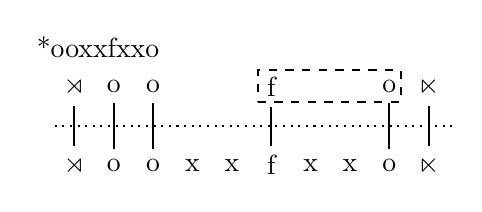
\begin{tikzpicture}
\node (1) at (0,0) {$\rtimes$};
\node (2) at (0.5,0) {o};
\node (3) at (1,0) {o};
\node (4) at (1.5,0) {x};
\node (5) at (2,0) {x};
\node (6) at (2.5,0) {f};
\node (7) at (3,0) {x};
\node (8) at (3.5,0) {x};
\node (9) at (4,0) {o};
\node (10) at (4.5,0) {$\ltimes$};
%
\node (01) at (0,1) {$\rtimes$};
\node (02) at (0.5,1) {o};
\node (03) at (1,1) {o};
\node (06) at (2.5,1) {f};
\node (09) at (4,1) {o};
\node (010) at (4.5,1) {$\ltimes$};
%
\foreach \Source/\Target in {%
	1.north/01.south,
	2.north/02.south,
	3.north/03.south,
	6.north/06.south,
	9.north/09.south,
	10.north/010.south%
    }
\draw (\Source) to (\Target);
%
\draw[dotted] (-0.25,0.5) to (4.8,0.5);
%
\node at (0.3,1.5) {*ooxxfxxo};
%
\draw [dashed] (2.33,0.81) -- (4.15,0.81) -- (4.15,1.21) -- (2.33,1.21) -- (2.33,0.81);
\end{tikzpicture}
\hspace{3em}
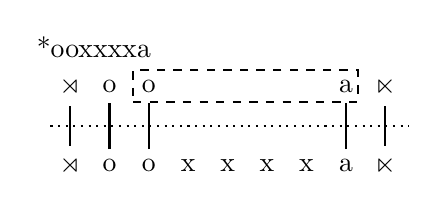
\begin{tikzpicture}
\node (1) at (0,0) {$\rtimes$};
\node (2) at (0.5,0) {o};
\node (3) at (1,0) {o};
\node (4) at (1.5,0) {x};
\node (5) at (2,0) {x};
\node (7) at (2.5,0) {x};
\node (8) at (3,0) {x};
\node (9) at (3.5,0) {a};
\node (10) at (4,0) {$\ltimes$};
%
\node (01) at (0,1) {$\rtimes$};
\node (02) at (0.5,1) {o};
\node (03) at (1,1) {o};
\node (09) at (3.5,1) {a};
\node (010) at (4,1) {$\ltimes$};
%
\foreach \Source/\Target in {%
	1.north/01.south,
	2.north/02.south,
	3.north/03.south,
	9.north/09.south,
	10.north/010.south%
    }
\draw (\Source) to (\Target);
%
\draw[dotted] (-0.25,0.5) to (4.3,0.5);
%
\node at (0.3,1.5) {*ooxxxxa};
%
\draw [dashed] (0.8,0.81) -- (3.65,0.81) -- (3.65,1.21) -- (0.8,1.21) -- (0.8,0.81);
\end{tikzpicture}
\end{center}
\caption{The extracted TSL grammar evaluating strings (Experiment $3$)}
\label{sgmnsge}
\end{figure}

\paragraph{Experiment 4: several vowel harmonies without blocking}

The learner induced that the ``consonant'' $x$ is not relevant for the vowel harmony system, and it also learned that on the tier of vowels, no disagreeing vowels can appear next to each other.
This learning outcome is therefore similar to the one of the second experiment, but with $4$ harmonic classes inferred instead of $2$.
This TSL grammar only generates words that are well-formed with respect to the rules of the vowel harmony  thus scoring $100$\% accuracy.

\begin{table}[h!]
\centering
\resizebox{\linewidth}{!}{%
\begin{tabular}{|r|l|}
\hline
\textbf{Pattern}            & \textit{several vowel harmonies, no blockers} \\ \hline
\textbf{Type of data}       & artificial data \\ \hline
\textbf{Example of data}    & xuuuxxxuuu, xxxeeexeee, xxxaaxxxaa, xoooxooxox, ... \\ \hline
%\textbf{Learned tier} & a, e, o, u  \\ \hline
\textbf{Learned $2$-TSL grammar} & (a, e, o, u)$_T$: ae, ao, ua, ue, uo, ... \\ \hline
\textbf{Generated sample}   & xxxaxaxaxax, xexxxexx, xxuxx, oxoxxox, ...\\ \hline
\textbf{Evaluation}         & \texttt{harmonic\_evaluator(sample, double\_harmony)} \\ \hline
\textbf{Score}              & $100$\%  \\ \hline
\end{tabular}}
\caption{TSL learning of several vowel harmonies without blockers; abstract representation.}
\end{table}


\paragraph{Experiment 5: several vowel harmonies with blocking}

The TSL learner correctly built a model for a Turkish-style harmonic system.
One tier is, indeed, able to capture both spreadings at the same time.
Given the tier consisting of all the vowels, the backness harmony can be expressed by a set of constraints of the type {[}$\alpha$front{]}{[}$-\alpha$front{]} (\emph{\"uu}, \emph{u\"u}, \emph{ae}, \emph{ea}, \emph{\"ua}, ...), and the rounding harmony that is blocked by non-high vowels is generalized as restrictions of the shape {[}$\alpha$round{]}{[}$-$high,$+$round{]} (\emph{oo}, \emph{uo}, \emph{eo}, ...) and {[}$\alpha$round{]}{[}$-\alpha$round, $+$high{]} (\emph{\"oi}, \emph{o\textsci}, \emph{au}, ...).
The performance of such model is $100$\%.

\begin{table}[h!]
\centering
\resizebox{\linewidth}{!}{%
\begin{tabular}{|r|l|}
\hline
\textbf{Pattern}            & \textit{several vowel harmonies with blockers} \\ \hline
\textbf{Type of data}       & artificial data \\ \hline
\textbf{Example of data}    & xx\"oexxix, xx\"u\"ux\"u\"ux, exxiixee, iiexxxex, xuuxxuuu, ... \\ \hline
%\textbf{Learned tier} & \textsci, \"o, \"u, a, e, i, o, u \\ \hline
\textbf{Learned $2$-TSL grammar} &  (\textsci, \"o, \"u, a, e, i, o, u)$_T$: \textsci\"o, \textsci\"u, \textsci e, \textsci i, \textsci o, ...\\ \hline
\textbf{Generated sample}   & xx\"oxxexx, x\textsci xxx, ax\textsci xxx, xaxxaxx, ...\\ \hline
\textbf{Evaluation}         & \texttt{harmonic\_evaluator(sample, backness\_and\_rounding)} \\ \hline
\textbf{Score}              & $100$\% overall ($100$\% backness only, $100$\% rounding only) \\ \hline
\end{tabular}
}
\caption{TSL learning of several harmonies with blockers; abstract representation.}
\end{table}

This result is theoretically expected since, in this pattern, there are two vowel harmonies happening at the same and affecting the same set of segments.
If we take two TSL grammars $G_1$ and $G_2$ that have the same tier alphabet but different sets of prohibited $n$-grams, taking a union of the prohibited $n$-grams would yield us another TSL grammar $G_3$.
Importantly, $G_3$ generates a language that is the intersection of the languages of $G_1$ and $G_2$.
To re-iterate this in more linguistic terms, \emph{two harmonies can fit on the same tier if the same sets of elements are involved in them}.




However, the learner did not perform well on the masked Turkish data.
It failed to remove $x$ from the tier since it did not observe \emph{\"o\"u} and \emph{ou} adjacent to each other, even though they are well-formed regarding the harmonic rules.
Its hypothesis, therefore, was not different from the one postulated by the SL grammar, and the accuracy of the model is $67$\%.

\begin{table}[h!]
\centering
\resizebox{\linewidth}{!}{%
\begin{tabular}{|r|l|}
\hline
\textbf{Pattern}            & \textit{several vowel harmonies with blockers} \\ \hline
\textbf{Type of data}       & masked Turkish data \\ \hline
\textbf{Example of data}    & xixxix, xuxx, xaaxa, xexxe, xax\textsci x, ... \\ \hline
%\textbf{Learned tier} & \textsci, \"o, \"u, a, e, i, o, u, x \\ \hline
\textbf{Learned $2$-TSL grammar} & (\textsci, \"o, \"u, a, e, i, o, u, x)$_T$: \textsci\"o, \textsci\"u, \textsci e, \textsci i, \textsci o, ...\\ \hline
\textbf{Generated sample}   & uux\"u\"ux, \"u, \textsci aaxeix, x\textsci\textsci\textsci\textsci x\"ue, ...\\ \hline
\textbf{Evaluation}         & \texttt{harmonic\_evaluator(sample, backness\_and\_rounding)} \\ \hline
\textbf{Score}              & $67$\% overall ($74$\% backness only, $74$\% rounding only) \\ \hline
\end{tabular}}
\caption{TSL learning of several harmonies with blockers; masked representation.}
\end{table}

The artificial dataset freely allowed vowel hiatus.
Harmonic vowels could be adjancent, such as in \emph{xxouxx}.
However, Turkish has gaps in what pairs of harmonic vowels can be adjacent in vowel hiatus.
Consequently, the performance of the TSL learner on the raw Turkish data was even worse, namely, $30$\%.



%The learner did not perform well on masked Turkish data, so, consequently, its performance was even worse on the raw data.
%Again, it failed to generalize the tier to a tier of vowels, and therefore was doing the same type of mistakes as the SL learner.
%Only $30$\% of the words predicted by the learned model were well-formed.



%
%\begin{table}[h!]
%\centering
%\begin{tabular}{|r|l|}
%\hline
%\textbf{Pattern}            & \textit{several vowel harmonies with blockers} \\ \hline
%\textbf{Type of data}       & raw Turkish data \\ \hline
%\textbf{Example of data}    & som, lafazan, konuk, kekti, lafzan, ... \\ \hline
%\textbf{Learned tier} & a, b, c, d, e, f, g, h, ... \\ \hline
%\textbf{Learned $2$-TSL grammar} & \u{g}o, \u{g}t, \u{g}v, \textsci\"o, \textsci\"u, ...\\ \hline
%\textbf{Generated sample}   & \"opoctal\textsci yov, sk, logsfig, eyu\c{c}m, ...\\ \hline
%\textbf{Evaluation}         & \texttt{harmonic\_evaluator(sample, backness\_and\_rounding)} \\ \hline
%\textbf{Score}              & $30$\% overall ($33$\% backness only, $35$\% rounding only) \\ \hline
%\end{tabular}
%\caption{TSL learning of several harmonies with blockers; raw representation}
%\end{table}


\subsection{Unsuccessful experiments}

TSL grammars can model patterns when a single set of elements is involved in a long-distance dependency.
However, if there is more than one long-distant process affecting different sets of elements, such as independent vowel and consonant harmonies, one tier is not enough.


\paragraph{Experiment 6: vowel harmony and consonant harmony without blocking}

It is impossible to model independent vowel and consonant harmonies using TSL grammars.
Vowels and consonants are involved in different long-distant processes, and therefore neither of them can be removed from the tier.
However, the presence of consonants does not allow us to represent vowels in a tier-based local fashion, and vice versa.
Therefore, neither vowel nor consonant harmony can be enforced: only $74$\% of the words generated by such grammar are well-formed.
This model is the same as its SL counterpart.

\begin{table}[h!]
\centering
\resizebox{\linewidth}{!}{%
\begin{tabular}{|r|l|}
\hline
\textbf{Pattern}            & \textit{vowel and consonant harmonies, no blockers} \\ \hline
\textbf{Type of data}       & artificial data \\ \hline
\textbf{Example of data}    & bbbaaabbaa, bbooboboob, pppoopppop, appaaappaa, ... \\ \hline
%\textbf{Learned tier} & a, b, o, p \\ \hline
\textbf{Learned $2$-TSL grammar} & (a, b, o, p)$_T$: ao, oa, bp, pb \\ \hline
\textbf{Generated sample}   & \textcolor{red!75!black}{apapoopop}, \textcolor{red!75!black}{oppoobbboopppob}, abab, \textcolor{red!75!black}{baaaap}, ...\\ \hline
\textbf{Evaluation}         & \texttt{harmonic\_evaluator(sample, double\_harmony\_no\_blockers)} \\ \hline
\textbf{Score}              & $74$\% \\ \hline
\end{tabular}}
\caption{TSL learning of vowel and consonant harmonies w/o blockers; abstract representation.}
\end{table}


\paragraph{Experiment 7: vowel harmony and consonant harmony with blocking}


Since TSL grammars failed to model the previous pattern with the independent vowel and consonant harmonies, they also fail to learn a similar pattern with a blocking effect.
Thus the performance of the TSL grammar, in this case, is again similar to its SL counterpart: $69$\%.


\begin{table}[h!]
\centering
\resizebox{\linewidth}{!}{%
\begin{tabular}{|r|l|}
\hline
\textbf{Pattern}            & \textit{vowel and consonant harmonies with blockers} \\ \hline
\textbf{Type of data}       & artificial data \\ \hline
\textbf{Example of data}    & pppoootopt, obbbtpooot, aabbbaatat, pppaapappp, ... \\ \hline
%\textbf{Learned tier} & a, b, o, p, t \\ \hline
\textbf{Learned $2$-TSL grammar} & (a, b, o, p, t)$_T$: ao, oa, bp, pb, tb \\ \hline
\textbf{Generated sample}   & \textcolor{red!75!black}{ptopaba}, btoptttpt, a, pppa, ob, ... \\ \hline
\textbf{Evaluation}         & \texttt{harmonic\_evaluator(sample, double\_harmony\_with\_blockers)} \\ \hline
\textbf{Score}              & $69$\% \\ \hline
\end{tabular}}
\caption{TSL learning of vowel and consonant harmonies with blockers; abstract representation.}
\end{table}


\paragraph{Experiment 8: unbounded tone plateauing}

There is no choice of a tier alphabet that would allow a TSL grammar to capture the \emph{no H...L...H} generalization.
If $H$ and $L$ are both present on the tier, such TSL grammar behaves like the SL one.
Otherwise either $H$ or $L$ needs to be omitted from the tier, but both of them are crucially important for the generalization.
Hence the pattern of UTP is neither SL nor TSL.
The learned grammar performs with the accuracy of $90$\% exclusively due to a small alphabet and the majority of the generated strings being short.

\begin{table}[h!]
\centering
\resizebox{\linewidth}{!}{%
\begin{tabular}{|r|l|}
\hline
\textbf{Pattern}            & \textit{unbounded tone plateauing} \\ \hline
\textbf{Type of data}       & artificial data \\ \hline
\textbf{Example of data}    & HHHHH, LHHLL, LHHHH, LHHHH, HHHHH, ... \\ \hline
%\textbf{Learned tier} & H, L \\ \hline
\textbf{Learned $3$-TSL grammar} & (H, L)$_T$: HLH \\ \hline
\textbf{Generated sample}   & \textcolor{red!75!black}{HHHLLH}, HLL, \textcolor{red!75!black}{HHLLHHLLLHLLLLLHHL}, LLLLH, ... \\ \hline
\textbf{Evaluation}         & \texttt{evaluate\_utp\_strings(sample)} \\ \hline
\textbf{Score}              & $90$\% \\ \hline
\end{tabular}}
\caption{TSL learning of unbounded tone plateauing; abstract representation.}
\end{table}


\paragraph{Experiment 9: first-last harmony}

As expected, the TSL learner cannot learn the unattested pattern of the first-last harmony.
In fact, the obtained grammar is the same as the one proposed by the SL learner, and therefore it makes exactly the same types of mistakes.

\begin{table}[h!]
\centering
\resizebox{\linewidth}{!}{%
\begin{tabular}{|r|l|}
\hline
\textbf{Pattern}            & \textit{first-last harmony} \\ \hline
\textbf{Type of data}       & artificial data \\ \hline
\textbf{Example of data}    & axoaaxaxaa, aaxaaxxxoa, ooaxaoaooo, axxoaxaaaa, ... \\ \hline
%\textbf{Learned tier} & a, o, x \\ \hline
\textbf{Learned $2$-TSL grammar} & (a, o, x)$_T$: \bow x, x\eow \\ \hline
\textbf{Generated sample}   & \textcolor{red!75!black}{aaoxaxxoxao}, aaxaooxa, \textcolor{red!75!black}{axooaao}, oxxo, ... \\ \hline
\textbf{Evaluation}         & \texttt{evaluate\_first\_last\_words(sample)} \\ \hline
\textbf{Score}              & $50$\% \\ \hline
\end{tabular}}
\caption{TSL learning of first-last harmony; abstract representation.}
\end{table}



\subsection{TSL experiments: interim summary}

A TSL learner, if given a representative sample of data, extracts a \emph{tier alphabet} that represents a set of elements involved in a long-distance dependency.
If every item of that set is also involved in another dependency, it can capture such cases as well, as it did in case of the abstract pattern of Turkish harmony.
Overall, TSL learner succeeded in building a grammar for every pattern that exhibited either a local dependency or a long-distance dependency among a single set of elements if given a representative sample.

However, if there is more than a single set of items involved in different long-distance dependencies, this cannot be modeled by TSL grammars.
Therefore TSL learner failed on a challenge that included learning separate vowel and consonant harmonies: for those cases, one tier is not enough.


\section{Multi-tier strictly local models}

Previous two sections explore two different perspectives on modeling long-distance dependencies.
Strictly piecewise grammars prohibit subsequences elements of which can be \emph{arbitrarily far} from each other.
SP models thus handle cases of multiple long-distance dependencies; however, none of them can include blockers.
Also, SP models can \emph{only} model long-distance dependencies: they cannot handle locally bounded patterns.
TSL grammars can encode local patterns and also blocking effects; however, they are limited to a \emph{single} set of items involved in a long-distance dependency.
Hence they cannot encode such cases as independent vowel and consonant harmonies within the same language.
In this section, I explore the performance of multi-tier strictly local (MTSL) models: namely, models that employ several TSL grammars at the same time.



\subsection{MTSL learning algorithm}
\label{mtsllearner}

The subregular class of MTSL grammars is a proper extension of TSL.
However, the $k$TSLIA algorithm introduced earlier cannot be simply extended from a single tier to multiple ones since its initial assumption is that \emph{all members of $\Sigma$} belong to a tier alphabet: it implicitly assumes the existence of just a single tier.

Together with Kevin McMullin and Aniello De Santo, we developed the MTSL learning algorithm \emph{MTSL$2$IA} \citep{McMullinAksenovaDeSanto2019}.
While there are several approaches to learning SL, SP, and TSL languages, MTSL$2$IA is the first published algorithm that tackles the problem of extracting MTSL grammars.
It relies on the assumption that we can first detect all the prohibited $k$-grams, and then learn a tier for every one of them .
Thus, we learn \emph{a tier for every negative bigram} of the MTSL grammar.
Currently, this algorithm only works with $2$-local restrictions, and the work of extending it to $k$ is ongoing.

Crucially, the MTSL$2$IA algorithm relies on the notion of a \emph{path} denoted as $\langle\rho_1, X, \rho_2\rangle$.
It can be thought of as a subsequence $(\rho_1\dots\rho_2)$ accompanied by a set of symbols $X$ that occurred in-between $\rho_1$ and $\rho_2$ in the training sample. For example, the following paths can be extracted from a string \emph{abac}:
$\langle a, \{\}, b \rangle$,
$\langle a, \{b\}, a \rangle$,
$\langle a, \{b, a\}, c \rangle$,
$\langle b, \{\}, a \rangle$,
$\langle b, \{a\}, c \rangle$, and 
$\langle b, \{\}, c \rangle$.


\begin{algorithm}
\caption{Extracts $G_{MTSL_{2}}$ from $I$}
\begin{algorithmic}
\REQUIRE a finite input sample $I \in \Sigma^*$
\STATE $B \leftarrow~ \Sigma^2 \cap \textrm{ngram}(I, 2)$
\STATE $i \leftarrow~ 1$
\FOR {$\rho_1\rho_2 \in~ B$}
	\STATE $R_i \leftarrow~ \rho_1\rho_2$
	\STATE $T_i \leftarrow~ \Sigma$
	\FOR {$\sigma \in~ \Sigma \cap \{\rho_1, \rho_2\}$}
		\IF {$\forall \langle\rho_1, X, \rho_2\rangle \in \textrm{path}(I) \textrm{ s.t. } \sigma\in~X, \langle\rho_1, X - \{\sigma\}, \rho_2\rangle~ \in \textrm{path}(I)$}
			\STATE $T_i \leftarrow~ T_i - \{\sigma\}$
		\ENDIF
	\ENDFOR
	\STATE $G_i \leftarrow~ \langle~ T_i, R_i \rangle$
	\STATE $i \leftarrow~ i+1$
\ENDFOR
\STATE $G \leftarrow~ G_1 \wedge G_2 \dots G_{\mid B\mid -1} \wedge G_{\mid B\mid}$
\RETURN $G$
\end{algorithmic}
\end{algorithm}

\textbf{Intuitively}, this algorithm works as follows.
At first, it detects a list of bigrams $B$ that is unattested in the training sample $I$.
Then it loops over all elements of $B$, and for every bigram $\rho_1\rho_2 \in~ B$, it assumes that the tier for that bigram is $\Sigma$.
Afterwards it collects a set of all paths of the form $\langle\rho_1, X, \rho_2\rangle$, and finds all symbols $\sigma \in~ \Sigma$ that can be removed from $X$ so that the newly obtained path $\langle\rho_1, X\setminus\{\sigma\}, \rho_2\rangle$ is still attested in the list of paths of $I$.
It then removes such $\sigma$ from a tier associated with $\rho_1\rho_2$.
After all members of $B$ were processed, the algorithm outputs a grammar $G$ that is a collection of all unattested bigrams with the tiers corresponding to those bigrams; see the \textbf{pseudocode} above.
Similarly to the learners discussed in the previous subsections, MTSL$2$IA learns the grammar from a positive sample in polynomial time and data \citep{McMullinAksenovaDeSanto2019}.

\paragraph{Example}
Imagine having a dataset that exhibits long-distance sibilant assimilation between \emph{\textesh} and \emph{s} unless blocked by \emph{f}.
Additionally, it also has vowel harmony affecting \emph{a} and \emph{o}.
This dataset includes the following strings: \emph{saasa, \textesh a\textesh aa, sooos, o\textesh o\textesh o, \textesh ofos, \textesh afas, sofo\textesh, safa\textesh, sf\textesh, sf\textesh,} and so on.
Of course, strings violating the rules of sibilant (such as \emph{\textesh aa\textesh as} or \emph{so\textesh ooa}) or vowel (\emph{a\textesh oo}, \emph{sosoa}) harmony are not included in the training sample.
As soon as the sample is given as input to the learner, the learner notices the absence of bigrams \emph{s\textesh , \textesh s, ao} and \emph{oa}.
When it explores the bigram \emph{s\textesh}, one of the paths to consider is $\langle s, \{a\}, \textrm{\textesh}\rangle$.
However, $\langle s, \{\}, \textrm{\textesh}\rangle$ is also a valid path, so \emph{a} is not a tier element for the bigram \emph{s\textesh}, and neither is \emph{o}.
When the unattested bigram \emph{ao} is explored, the learner does not detect any paths that would involve the symbols \{$s$, \textesh, $f$\}.
The condition of the if-statement is then trivially satisfied, and therefore \emph{s, \textesh} and \emph{f} are removed from the tier of that bigram.
A concise representation of the grammar that the learner induced is the following:

\begin{itemize}
	\item $G_1 = \langle T_1 = \{a, o\}, R_1 = \{ao, oa\}\rangle$;
	\item $G_2 = \langle T_2 = \{s, \textrm{\textesh}, f\}, R_2 = \{\textrm{\textesh}s, s\textrm{\textesh}\}\rangle$.
\end{itemize}

However, the \emph{tier-per-bigram} assumption comes with a caveat.
It results in the algorithm failing to capture patterns where the same bigram is present on several different tiers.
For example, consider an MTSL grammar where the bigram \emph{xx} is prohibited on two tiers: $T_1 = \{x, a\}$ and $T_2 = \{x, b\}$.
Instead, the MTSL$2$IA learner would converge on the incorrect tier $T = \{x, a, b\}$.
Tier configurations that cannot be learned by this learner is a sub-case of a general case when two tier alphabets have a non-empty intersection that does not overlap with either of the alphabets.
Interestingly, we show in \citet{AksenovaDeshmukh2018} that in natural languages, if two agreements require two different tiers, those tiers never overlap unless one of them is properly contained within the other one.
Therefore if applied to phonological data, this learner could be more efficient in comparison to the learner that would also explore the typologically unattested class of tier configurations.

As noted previously, this algorithm learns $2$-local MTSL grammars, but we are currently working on extending it to arbitrary $k$.
Intuitively, this can be done by extending the notion of a path.
Its shape could be generalized as $\langle\rho_1, X_1, \rho_2, X_2, \dots \rho_{n-1}, X_{n-1}, \rho_n\rangle$, where $\rho_1\rho_2\dots\rho_n$ is a $k$-long sequence, and $X_i$ is the set of symbols that occurred in-between $\rho_i$ and $\rho_{i+1}$ in the training sample.
The condition of the if-statement needs to also be adjusted to accommodate for longer paths; but otherwise, the logic of the algorithm stays the same.



\subsection{Successful experiments}

In this subsection, I show that MTSL grammars can be used to successfully model all of the discussed types of local processes and long-distant harmonies.
Even when challenged with the raw data of German, Finnish, and Turkish, the MTSL learner extracts the corresponding MTSL grammars with the impressive accuracies of $100$\%, $100$\%, and $95$\%, correspondingly.
The patterns of unbounded tone plateauing and the first-last harmony are not MTSL in their nature, and therefore cannot be learned using the MTSL inference algorithm.


\paragraph{Experiment 1: word-final devoicing}

Since MTSL grammars are a proper superclass of TSL grammars, and, consequently, of the SL ones, the MTSL learning algorithm acquires the pattern of word-final devoicing.
The performance of the MTSL model on the raw German dataset is $100$\%, as well as on the other representations of that pattern.

\begin{table}[h!]
\centering
\resizebox{\linewidth}{!}{%
\begin{tabular}{|r|l|}
\hline
\textbf{Pattern}            & \textit{word-final devoicing}  \\ \hline
\textbf{Type of data}       & raw German data \\ \hline
\textbf{Example of data}    & hochjagende, zugebliebener, verbricht, besuchszimmer, ... \\ \hline
\textbf{Learned $2$-MTSL grammar} & \emph{too large: $294$ tiers!} \\ \hline
\textbf{Generated sample}   & mugoftkuh\"ampo, kisizkkokg\"up, rk\"ums\"ubtal... \\ \hline
\textbf{Evaluation}         & \texttt{evaluate\_wfd\_words(sample)}   \\ \hline
\textbf{Score}              & $100$\%   \\ \hline
\end{tabular}}
\caption{MTSL learning of the word-final devoicing; raw representation.}
\end{table}


%
%\begin{table}[h!]
%\centering
%\begin{tabular}{|r|l|}
%\hline
%\textbf{Pattern}            & \textit{word-final devoicing} \\ \hline
%\textbf{Type of data}       & artificial data  \\ \hline
%\textbf{Example of data}    & aaabbpbbbp, pbapbapapa, apabaappap, bbbbaabbbp, ... \\ \hline
%\textbf{Learned $2$-MTSL grammar} & (a, b, p)$_T$: b\eow, \bow\eow  \\ \hline
%\textbf{Generated sample}   & pp, pbpapaba, bpppp, aap, bp, ...  \\ \hline
%\textbf{Evaluation}         & \texttt{evaluate\_wfd\_words(sample)} \\ \hline
%\textbf{Score}              & $100$\% \\ \hline
%\end{tabular}
%\caption{MTSL learning of the word-final devoicing; abstract representation}
%\end{table}

%\begin{table}[h!]
%\centering
%\begin{tabular}{|r|l|}
%\hline
%\textbf{Pattern}            & \textit{word-final devoicing}    \\ \hline
%\textbf{Type of data}       & masked German data \\ \hline
%\textbf{Example of data}    & aakaabaaaa, aakaabaaak, aakaa, aakat, aaa, ... \\ \hline
%\textbf{Learned $2$-MTSL grammar} & (a, b, d, g, k, p, t)$_T$: b\eow, d\eow, g\eow, \bow\eow              \\ \hline
%\textbf{Generated sample}   & agdgdbgkdapk, dptkp, pktbdkgtadpa, tgdgp, ... \\ \hline
%\textbf{Evaluation}         & \texttt{evaluate\_wfd\_words(sample)} \\ \hline
%\textbf{Score}              & $100$\%  \\ \hline
%\end{tabular}
%\caption{MTSL learning of the word-final devoicing; masked representation}
%\end{table}




\paragraph{Experiment 2: a single vowel harmony without blocking}

Similarly, the MTSL learner extracted the grammar representing a single vowel harmony pattern without a blocking effect.
The learner induced a single tier containing symbols $a$ and $o$.
The grammar for this tier was the same one as in the TSL version of this experiment: $ao$, $oa$.
$100$\% of the words generated by the obtained grammar were well-formed.
The success of the MTSL learner on this and further experiments where the TSL learner performed well follows from the fact that the class of MTSL languages subsumes TSL languages. 


\begin{table}[h!]
\centering
\resizebox{\linewidth}{!}{%
\begin{tabular}{|r|l|}
\hline
\textbf{Pattern}            & \textit{one vowel harmony, no blockers} \\ \hline
\textbf{Type of data}       & artificial data \\ \hline
\textbf{Example of data}    & oxxxooxxxx, ooxxxooxxo, aaxxxaaxxx, oxxxxoxxxo, ... \\ \hline
\textbf{Learned $2$-MTSL grammar} & (a, o)$_T$: ao, oa \\ \hline
\textbf{Generated sample}   & xxoox, xxaxaxa, axaaax, xooox, ... \\ \hline
\textbf{Evaluation}         & \texttt{harmonic\_evaluator(sample, single\_harmony\_no\_blockers)}  \\ \hline
\textbf{Score}              & $100$\%   \\ \hline
\end{tabular}}
\caption{MTSL learning of a single harmony without blockers; abstract representation.}
\end{table}

%\begin{table}[h!]
%\centering
%\begin{tabular}{|r|l|}
%\hline
%\textbf{Pattern}            & \textit{one vowel harmony, no blockers}  \\ \hline
%\textbf{Type of data}       & masked Finnish data \\ \hline
%\textbf{Example of data}    & xaxxixxex, xix\"axixex, xaxxixxaxix, uxxuxaxxix, ... \\ \hline
%\textbf{Learned $2$-MTSL grammar} & \begin{tabular}[c]{@{}l@{}}
%(u, y)$_T$: yu, uy; 
%(\"a, u)$_T$: \"au, u\"a; 
%(\"o, o)$_T$: \"oo, o\"o; etc.
%\end{tabular} \\ \hline
%\textbf{Generated sample}   & \"oyxy\"a\"o\"oyyy\"o, \"oyxy\"a\"o, \"ayx, oxxuxaxu, ... \\ \hline
%\textbf{Evaluation}         & \texttt{harmonic\_evaluator(sample, front\_harmony)}   \\ \hline
%\textbf{Score}              & $100$\%  \\ \hline
%\end{tabular}
%\caption{MTSL learning of a single harmony without blockers; masked representation}
%\end{table}

The MTSL inference algorithm also successfully learned the generalization from raw and masked Finnish datasets.
Indeed, $100$\% of the words generated by the grammar, such as \emph{rjegovnj} or \emph{l\"ay\"omppl}, are harmonic.
Although the grammar is transparent and fully interpretable, it postulates $266$ tiers.
An open question is to explain \emph{how exactly} increasing the number of tiers helped the learner to tackle this challenge.


\begin{table}[h!]
\centering
\resizebox{\linewidth}{!}{%
\begin{tabular}{|r|l|}
\hline
\textbf{Pattern}            & \textit{one vowel harmony, no blockers}  \\ \hline
\textbf{Type of data}       & raw Finnish data \\ \hline
\textbf{Example of data}    & mathilden, lis\"animen, macmillanin, urquhartin, ... \\ \hline
\textbf{Learned $2$-MTSL grammar} & \emph{too large: $266$ tiers!} \\ \hline
\textbf{Generated sample}   & rjegovnj, l\"ay\"omppl, axiflt, sil\"o\"a\"amydv, ... \\ \hline
\textbf{Evaluation}         & \texttt{harmonic\_evaluator(sample, front\_harmony)} \\ \hline
\textbf{Score}              & $100$\%  \\ \hline
\end{tabular}}
\caption{MTSL learning of a single harmony without blockers; raw representation.}
\end{table}



\paragraph{Experiment 3: a single vowel harmony with blocking}

Again, the success of the MTSL learner in this experiment follows from the fact that TSL grammars are a proper subset of the MTSL ones.
However, what is surprising is that the MTSL inference algorithm did not converge on a single tier: instead, it postulated $3$ different tiers.

The learner discovered $3$ unattested bigrams: $ao$, $fo$, and $oa$.
However, in none of the data points $a$ was ever followed by $o$, so there were no paths of the type $\langle a, X, o\rangle$: trivially, elements $f$ and $x$ were considered irrelevant for this restriction.
Similarly, $a$ was excluded from a tier induced for the restriction $fo$ because $f$ is never followed by $o$.
But when considering the unattested bigram $oa$, paths such as $\langle o, \{f\}, a\rangle$ and $\langle o, \{f, x\}, a\rangle$ were found in the data, while the ones such as $\langle o, \{\}, a\rangle$ were not.
A symbol $x$ was hence removed from the tier of the bigram $oa$, but the blocker $f$ was not.
In such a way, MTSL learner constructs $3$ different tiers, but the language of the obtained grammar is equivalent to the one of the TSL grammar $\{oa, ao, fo\}$ with the tier $T = \{a, o, f\}$.

\begin{table}[h!]
\centering
\resizebox{\linewidth}{!}{%
\begin{tabular}{|r|l|}
\hline
\textbf{Pattern}            & \textit{one vowel harmony with blockers} \\ \hline
\textbf{Type of data}       & artificial data \\ \hline
\textbf{Example of data}    & oxxxooxxxx, xxooxfaaax, aaxxxaaxxx, ofxxafxxaa, ... \\ \hline
\textbf{Learned $2$-MTSL grammar} & \begin{tabular}[c]{@{}l@{}}
(a, o)$_T$: ao; 
(f, o)$_T$: fo; 
(a, f, o)$_T$: oa.
\end{tabular} \\ \hline
\textbf{Generated sample}   & oxffxax, faaaxffa, ofxaaf, fa, ooooof, ...\\ \hline
\textbf{Evaluation}         & \texttt{harmonic\_evaluator(sample, single\_harmony\_with\_blockers)}    \\ \hline
\textbf{Score}              & $100$\%  \\ \hline
\end{tabular}}
\caption{MTSL learning of a single harmony with blockers; abstract representation.}
\end{table}


\paragraph{Experiment 4: several vowel harmonies without blocking}

This experiment was successful since the MTSL learner extracted the grammar for the pattern of several vowel harmonies without a blocking effect.
However, similarly to the previous example, the resulting grammar was not the same as the one extracted by the TSL learner.
The MTSL algorithm constructed a separate tier for every pair of the potentially disagreeing elements, while correctly noticing that the transparent element $x$ is irrelevant for the generalization.

\begin{table}[h!]
\centering
\resizebox{\linewidth}{!}{%
\begin{tabular}{|r|l|}
\hline
\textbf{Pattern}            & \textit{several vowel harmonies, no blockers} \\ \hline
\textbf{Type of data}       & artificial data \\ \hline
\textbf{Example of data}    & xuuuxxxuuu, xxxeeexeee, xxxaaxxxaa, xoooxooxox, ... \\ \hline
\textbf{Learned $2$-MTSL grammar} & \begin{tabular}[c]{@{}l@{}}
(u, o)$_T$: uo, ou; 
(a, u)$_T$: au, ua; 
(o, e)$_T$: eo, oe; etc.
\end{tabular} \\ \hline
\textbf{Generated sample}   & xuxuuuxu, xoox, aaa, exexxe ...\\ \hline
\textbf{Evaluation}         & \texttt{harmonic\_evaluator(sample, double\_harmony)} \\ \hline
\textbf{Score}              & $100$\%  \\ \hline
\end{tabular}}
\caption{MTSL learning of several vowel harmonies without blockers; abstract representation.}
\end{table}



\paragraph{Experiment 5: several vowel harmonies with blocking}

The MTSL induction algorithm found a way to model several vowel harmonies with a blocking effect.
Also, similarly to the examples discussed above, more than a single tier was inferred.
All of the words generated by the extracted MTSL grammar were well-formed regarding the rules of Turkish harmony.

\begin{table}[h!]
\centering
\resizebox{\linewidth}{!}{%
\begin{tabular}{|r|l|}
\hline
\textbf{Pattern}            & \textit{several vowel harmonies with blockers} \\ \hline
\textbf{Type of data}       & artificial data \\ \hline
\textbf{Example of data}    & xx\"oexxix, xx\"u\"ux\"u\"ux, exxiixee, iiexxxex, xuuxxuuu, ... \\ \hline
\textbf{Learned $2$-MTSL grammar} & \begin{tabular}[c]{@{}l@{}}
(\"u, e, i)$_T$: \"ui; 
(\"u, e)$_T$: e\"u; 
(\textsci, \"o)$_T$: \textsci\"o, \"o\textsci; etc.
\end{tabular} \\ \hline
\textbf{Generated sample}   & \textsci xxaaaa, \"uexi, \"uxeexe, \"o\"u\"u\"ue, \"o\"uexe, ... \\ \hline
\textbf{Evaluation}         & \texttt{harmonic\_evaluator(sample, backness\_and\_rounding)} \\ \hline
\textbf{Score}              & $100$\% overall ($100$\% backness only, $100$\% rounding only) \\ \hline
\end{tabular}}
\caption{MTSL learning of several harmonies with blockers; abstract representation.}
\end{table}


Some of the configurations that the MTSL learner was looking for were missing in the masked and raw representations of the Turkish data, and therefore the accuracies of those models were slightly worse than ideal: both of them scored $95$\%.
As of the MTSL grammar inferred from the raw data, it relies on $266$ tiers, and the way it is able to perform so well is worth further investigation.

%\begin{table}[h!]
%\centering
%\begin{tabular}{|r|l|}
%\hline
%\textbf{Pattern}            & \textit{several vowel harmonies with blockers} \\ \hline
%\textbf{Type of data}       & masked Turkish data \\ \hline
%\textbf{Example of data}    & xixxix, xuxx, xaaxa, xexxe, xax\textsci x, ... \\ \hline
%\textbf{Learned $2$-MTSL grammar} & \begin{tabular}[c]{@{}l@{}}
%(\"u, e, i, x)$_T$: \"ui; 
%(\"u, o, x)$_T$: \"o\"u; 
%(\"u, e)$_T$: \"ue; etc.
%\end{tabular} \\ \hline
%\textbf{Generated sample}   & \"uxxeeee, xox\textsci a\textsci, exxxeixixei, ux\textsci xxa, ...\\ \hline
%\textbf{Evaluation}         & \texttt{harmonic\_evaluator(sample, backness\_and\_rounding)} \\ \hline
%\textbf{Score}              & $95$\% overall ($100$\% backness only, $95$\% rounding only) \\ \hline
%\end{tabular}
%\caption{MTSL learning of several harmonies with blockers; masked representation}
%\end{table}

\begin{table}[h!]
\centering
\resizebox{\linewidth}{!}{%
\begin{tabular}{|r|l|}
\hline
\textbf{Pattern}            & \textit{several vowel harmonies with blockers} \\ \hline
\textbf{Type of data}       & raw Turkish data \\ \hline
\textbf{Example of data}    & som, lafazan, konuk, kekti, lafzan, ... \\ \hline
\textbf{Learned $2$-MTSL grammar} &  \emph{too large: $266$ tiers!} \\ \hline
\textbf{Generated sample}   & apn\textsci c\textsci r\textsci saa,  tel\c{c}it\c{c}eeriden, mbezkdenic, ...\\ \hline
\textbf{Evaluation}         & \texttt{harmonic\_evaluator(sample, backness\_and\_rounding)} \\ \hline
\textbf{Score}              & $95$\% overall ($100$\% backness only, $95$\% rounding only) \\ \hline
\end{tabular}}
\caption{MTSL learning of several harmonies with blockers; raw representation.}
\end{table}


\paragraph{Experiment 6: vowel harmony and consonant harmony without blocking}

The pattern of independent vowel and consonant harmonies can be captured using two tiers: one for vowels, and another one for consonants.
The tier of vowels prohibits $oa$ and $ao$, and the tier of consonants rules out $pb$ and $bp$.
To evaluate the well-formedness of a word, both of its tiers need to be inspected individually.
For example, consider a word \emph{ababbabb}.
Tts consonant tier contains \emph{bbbbb}, and the vowel tier is \emph{aaa}: both of them are well-formed.
However, words such as \emph{ababbbob} are not grammatical: even though the consonant tier does not contain violations, the vowel tier is \emph{a\textbf{ao}}, and it violates the rules of the vowel harmony.
The language of this MTSL grammar is the intersection of two TSL grammars, one per every harmony.
The accuracy of this model is $100$\%.

\begin{table}[h!]
\centering
\resizebox{\linewidth}{!}{%
\begin{tabular}{|r|l|}
\hline
\textbf{Pattern}            & \textit{vowel and consonant harmonies, no blockers} \\ \hline
\textbf{Type of data}       & artificial data \\ \hline
\textbf{Example of data}    & bbbaaabbaa, bbooboboob, pppoopppop, appaaappaa, ... \\ \hline
\textbf{Learned $2$-MTSL grammar} & \begin{tabular}[c]{@{}l@{}}
(a, o)$_T$: ao, oa; 
(b, p)$_T$: pb, bp.
\end{tabular} \\ \hline
\textbf{Generated sample}   & oapapaaa, obbb, babbba, poop, ...\\ \hline
\textbf{Evaluation}         & \texttt{harmonic\_evaluator(sample, double\_harmony\_no\_blockers)} \\ \hline
\textbf{Score}              & $100$\% \\ \hline
\end{tabular}}
\caption{MTSL learning of vowel and consonant harmonies w/o blockers; abstract representation.}
\end{table}


\paragraph{Experiment 7: vowel harmony and consonant harmony with blocking}

MTSL learner performs $100$\% accurate on the pattern with vowel and consonant harmonies even if they include blockers, and it is the only subregular model among the discussed ones that is able to do so.
In this case, the learner extracts $4$ tiers, and a total of $5$ prohibited bigrams.
The choice of the tiers can be explained in the same way it was done for the third experiment.
On the tier of vowels, the grammar prohibits their disagreeing combinations $ao$ and $oa$.
The consonant-related restrictions are located across $3$ different tiers due to the inference steps of the algorithm, but these restrictions, in fact, can be expressed on a single tier containing $p$, $b$, and $t$.
Figure \ref{fakjfanfk} shows the MTSL evaluation of strings \emph{aabbotoob} and \emph{aabbaaaap} using a simplified yet equivalent MTSL grammar containing only $2$ tiers: one for vowels, and another for consonants.

\begin{table}[h!]
\centering
\resizebox{\linewidth}{!}{%
\begin{tabular}{|r|l|}
\hline
\textbf{Pattern}            & \textit{vowel and consonant harmonies with blockers} \\ \hline
\textbf{Type of data}       & artificial data \\ \hline
\textbf{Example of data}    & pppoootopt, obbbtpooot, aabbbaatat, pppaapappp, ... \\ \hline
\textbf{Learned $2$-MTSL grammar} & \begin{tabular}[c]{@{}l@{}}
(b, p, t)$_T$: bp; 
(a, o)$_T$: ao, oa;
(b, p)$_T$: pb;
(b, t)$_T$: tb.
\end{tabular} \\ \hline
\textbf{Generated sample}   & obtppoppo, totoo, ap, ooptpp, abtatat, ... \\ \hline
\textbf{Evaluation}         & \texttt{harmonic\_evaluator(sample, double\_harmony\_with\_blockers)} \\ \hline
\textbf{Score}              & $100$\% \\ \hline
\end{tabular}}
\caption{MTSL learning of vowel and consonant harmonies with blockers; abstract representation.}
\end{table}

\begin{figure}[h!]
\begin{center}
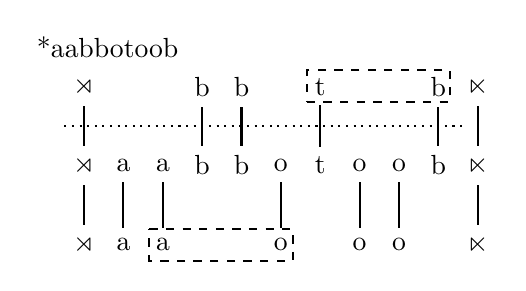
\begin{tikzpicture}
\node (1) at (0,0) {$\rtimes$};
\node (2) at (0.5,0) {a};
\node (3) at (1,0) {a};
\node (4) at (1.5,0) {b};
\node (5) at (2,0) {b};
\node (6) at (2.5,0) {o};
\node (7) at (3,0) {t};
\node (8) at (3.5,0) {o};
\node (9) at (4,0) {o};
\node (10) at (4.5,0) {b};
\node (11) at (5,0) {$\ltimes$};
%
\node (001) at (0,-1) {$\rtimes$};
\node (002) at (0.5,-1) {a};
\node (003) at (1,-1) {a};
\node (006) at (2.5,-1) {o};
\node (008) at (3.5,-1) {o};
\node (009) at (4,-1) {o};
\node (0011) at (5,-1) {$\ltimes$};
%
\node (01) at (0,1) {$\rtimes$};
\node (04) at (1.5,1) {b};
\node (05) at (2,1) {b};
\node (07) at (3,1) {t};
\node (010) at (4.5,1) {b};
\node (011) at (5,1) {$\ltimes$};
%
\foreach \Source/\Target in {%
	1.north/01.south,
	4.north/04.south,
	5.north/05.south,
	7.north/07.south,
	11.north/011.south,
	10.north/010.south%
    }
\draw (\Source) to (\Target);
%
\foreach \Source/\Target in {%
	001.north/1.south,
	002.north/2.south,
	003.north/3.south,
	006.north/6.south,
	008.north/8.south,
	009.north/9.south,
	0011.north/11.south%
    }
\draw (\Source) to (\Target);
%
\draw[dotted] (-0.25,0.5) to (4.8,0.5);
%
\node at (0.3,1.5) {*aabbotoob};
%
\draw [dashed] (2.83,0.81) -- (4.65,0.81) -- (4.65,1.21) -- (2.83,1.21) -- (2.83,0.81);
\draw [dashed] (0.83,-0.81) -- (2.65,-0.81) -- (2.65,-1.21) -- (0.83,-1.21) -- (0.83,-0.81);
\end{tikzpicture}
\hspace{3em}
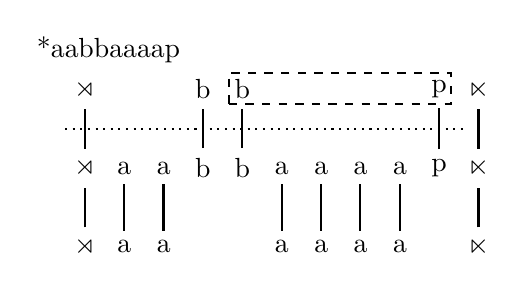
\begin{tikzpicture}
\node (1) at (0,0) {$\rtimes$};
\node (2) at (0.5,0) {a};
\node (3) at (1,0) {a};
\node (4) at (1.5,0) {b};
\node (5) at (2,0) {b};
\node (6) at (2.5,0) {a};
\node (7) at (3,0) {a};
\node (8) at (3.5,0) {a};
\node (9) at (4,0) {a};
\node (10) at (4.5,0) {p};
\node (11) at (5,0) {$\ltimes$};
%
\node (001) at (0,-1) {$\rtimes$};
\node (002) at (0.5,-1) {a};
\node (003) at (1,-1) {a};
\node (006) at (2.5,-1) {a};
\node (007) at (3,-1) {a};
\node (008) at (3.5,-1) {a};
\node (009) at (4,-1) {a};
\node (0011) at (5,-1) {$\ltimes$};
%
\node (01) at (0,1) {$\rtimes$};
\node (04) at (1.5,1) {b};
\node (05) at (2,1) {b};
\node (010) at (4.5,1) {p};
\node (011) at (5,1) {$\ltimes$};
%
\foreach \Source/\Target in {%
	1.north/01.south,
	4.north/04.south,
	5.north/05.south,
	11.north/011.south,
	10.north/010.south%
    }
\draw (\Source) to (\Target);
%
\foreach \Source/\Target in {%
	001.north/1.south,
	002.north/2.south,
	003.north/3.south,
	006.north/6.south,
	007.north/7.south,
	008.north/8.south,
	009.north/9.south,
	0011.north/11.south%
    }
\draw (\Source) to (\Target);
%
\draw[dotted] (-0.25,0.5) to (4.8,0.5);
%
\node at (0.3,1.5) {*aabbaaaap};
%
\draw [dashed] (1.83,0.81) -- (4.65,0.81) -- (4.65,1.21) -- (1.83,1.21) -- (1.83,0.81);
\end{tikzpicture}
\end{center}
\caption{Experiment $7$: the extracted MTSL grammar evaluating the ungrammatical strings \emph{aabbotoob} and \emph{aabbaaaap}.}
\label{fakjfanfk}
\end{figure}



\subsection{Unsuccessful experiments}

I was not able to test the performance of the MTSL learner on the UTP pattern since this learner currently exists only for $2$-local dependencies, and UTP requires postulating a $3$-local restriction.
However, this pattern is not MTSL expressible since there is no tier or a combination of tiers that would be able to express that generalization.
Hence the only unsuccessful experiment that I present in this subsection is the expected inability of MTSL grammars to express the first-last harmony.


\paragraph{Experiment 9: first-last harmony}

MTSL grammars cannot encode the pattern of the first-last harmony.
The MTSL learner extracts exactly the same grammar as TSL and SL learners: it only notices that the ``non-agreeing'' item $x$ cannot occur string-initially and string-finally.
It fails to generalize that the string-initial and string-final symbols need to match, and therefore the accuracy of this model is $50$\%.

\begin{table}[h!]
\centering
\resizebox{\linewidth}{!}{%
\begin{tabular}{|r|l|}
\hline
\textbf{Pattern}            & \textit{first-last harmony} \\ \hline
\textbf{Type of data}       & artificial data \\ \hline
\textbf{Example of data}    & axoaaxaxaa, aaxaaxxxoa, ooaxaoaooo, axxoaxaaaa, ... \\ \hline
\textbf{Learned $2$-MTSL grammar} & (a, o, x)$_T$: \bow x, x\eow \\ \hline
\textbf{Generated sample}   & \textcolor{red!75!black}{ooaaa}, aaoa, \textcolor{red!75!black}{ooooaxxa}, oaaaxao, ...
 \\ \hline
\textbf{Evaluation}         & \texttt{evaluate\_first\_last\_words(sample)} \\ \hline
\textbf{Score}              & $50$\% \\ \hline
\end{tabular}}
\caption{MTSL learning of first-last harmony; abstract representation.}
\end{table}


\subsection{MTSL experiments: interim summary}

The MTSL learner successfully extracted MTSL grammars corresponding to all types of harmonic systems present in the list of the experiments, performing equally well on cases with or without the blocking effect.
While being able to capture long-distance dependencies, it also performed extremely well on the local pattern of word-final devoicing.
Importantly, apart from learning the patterns from the artificially generated datasets, it also was able to generalize the rules from the raw data, scoring $100$\% on German and Finnish, and $95$\% on Turkish datasets.
The experiment using the non-MTSL pattern of unbounded tone plateauing is not discussed due to the unavailability of the $3$-local MTSL learner at the current moment.
Finally, as expected, the first-last harmony is not learnable by either of the discussed subregular learners.


However, as explained before in section \ref{mtsllearner}, there is a type of MTSL grammars that the current learner cannot induce due to its tier-per-bigram assumption.
Namely, it cannot learn an MTSL grammar where one bigram belongs to two different tiers.
Interestingly, according to \cite{AksenovaDeshmukh2018}, languages with multiple harmonies typologically lack this type of tier configuration.
Therefore this learner could be more efficient for language-related tasks then the one that would investigate typologically unattested possibilities.


\section{Learning languages: summary}
\label{interimsummarylanguages}

In this chapter, I discussed possibilities of modeling natural language patterns using subregular methods.
Namely, I explored the performance of strictly piecewise (SP), strictly local (SL), tier-based strictly local (TLS), and multi-tier strictly local (MTSL) learning algorithms using different datasets exhibiting natural language dependencies.
The experiments ranged from ones that were using artificially generated samples imitating linguistic patterns, to extracting grammars from raw language data.
Artificial language learning shows if the modeling of those generalizations is possible \emph{conceptually}, whereas using raw data shows what is possible \emph{in practice}.

The discussed learning experiments targeted following patterns: word-final devoicing, a single vowel harmony pattern with/without a blocking effect, several vowel harmonies with/without a blocking effect, independent vowel and consonant harmonies with/without blocking effect, and the unbounded tone plateauing.
Additionally, I also challenged the learners with a typologically unattested pattern of first-last harmony.
Every one among these $9$ patterns can be theoretically modeled using different set of subregular classes.
Namely, word-final devoicing can be captured by SL, TSL, and MTSL grammars; several vowel harmonies with blocking are expressible by TSL and MTSL grammars, and the unbounded tone plateauing can only be encoded using a SP grammar.
Finally, none of the subregular languages should be able to capture the first-last harmony since it is not SL, SP, TSL, or MTSL.
In \ref{explanglearn2}, I repeat the table with the expected results of the language learning experiments that was previously shown in \ref{explanglearn}.


\begin{table}[b!]
\begin{center}
\resizebox{\linewidth}{!}{%
\begin{tabular}{|r|c|c|c|c|}
\hline
\multicolumn{1}{|c|}{\textbf{Target patterns}}           & \multicolumn{1}{l|}{\textbf{SP}} & \multicolumn{1}{l|}{\textbf{SL}} & \multicolumn{1}{l|}{\textbf{TSL}} & \multicolumn{1}{l|}{\textbf{MTSL}} \\ \hline
\textit{word-final devoicing}                            & \cellcolor{gray!50}\faTimes                               & \faThumbsOUp                                & \faThumbsOUp                                 & \faThumbsOUp                                  \\ \hline
\textit{a single vowel harmony without blocking}               & \faThumbsOUp                                & \cellcolor{gray!50}\faTimes                                & \faThumbsOUp                                 & \faThumbsOUp                                  \\ \hline
\textit{a single vowel harmony with blocking}              & \cellcolor{gray!50}\faTimes                                & \cellcolor{gray!50}\faTimes                                & \faThumbsOUp                                 & \faThumbsOUp                                  \\ \hline
\textit{several vowel harmonies without blocking}              & \faThumbsOUp                                & \cellcolor{gray!50}\faTimes                                & \faThumbsOUp                                 & \faThumbsOUp                                  \\ \hline
\textit{several vowel harmonies with blocking}              & \cellcolor{gray!50}\faTimes                                & \cellcolor{gray!50}\faTimes                                & \faThumbsOUp                                 & \faThumbsOUp                                  \\ \hline
\textit{vowel harmony and consonant harmony without blocking}  & \faThumbsOUp                                & \cellcolor{gray!50}\faTimes                                & \cellcolor{gray!50}\faTimes                                 & \faThumbsOUp                                  \\ \hline
\textit{vowel harmony and consonant harmony with blocking} &\cellcolor{gray!50} \faTimes                               &\cellcolor{gray!50} \faTimes                                &\cellcolor{gray!50} \faTimes                                 & \faThumbsOUp                                  \\ \hline
\textit{unbounded tone plateauing}                       & \faThumbsOUp                                &\cellcolor{gray!50} \faTimes                                & \cellcolor{gray!50}\faTimes                                 &\cellcolor{gray!50} \faTimes                                  \\ \hline
\textit{first-last harmony}                              & \cellcolor{gray!50}\faTimes                                &\cellcolor{gray!50} \faTimes                                &\cellcolor{gray!50} \faTimes                                 & \cellcolor{gray!50}\faTimes                                  \\ \hline
\end{tabular}}
\end{center}
\caption{The expected results of the language learning experiments; repeated from the end of the section 3.1.4.}
\label{explanglearn2}
\end{table}

Every experiment included $4$ steps: data colleciton or generation, subregular learning, sample generation using the constructed grammar, and model evaluation.
At first, I prepared the \emph{training samples}. 
They range from the automatically generated artificial languages, to simplified (masked) representations of the natural language data, to wordlists of German, Finnish and Turkish.
During the \emph{learning} step, a grammar was obtained by the inference algorithm based on the provided training data.
Then I \emph{generated} a large set of strings that are grammatical according to the extracted grammar.
Finally, I computed the number of strings of the generated sample that are well-formed according to the target generalization thus numerically \emph{evaluating} the performance of the model.
The table \ref{languagesresults} summarizes how the automatically extracted subregular grammars performed on those experiments.


{\small
\begin{table}[h!]
\begin{center}
\scalebox{0.7}{%
\begin{tabular}{|r|c|c|c|c|}
\hline
\multicolumn{1}{|c|}{\textbf{Data}}   & \textbf{SP}   & \textbf{SL}  & \textbf{TSL}  & \textbf{MTSL}  \\ \hline
\multicolumn{5}{|l|}{\cellcolor{gray!30!white}\textit{\textbf{Experiment 1: word-final devoicing}}}                                 \\ \hline
Theoretical expectations  & \faTimes & \faThumbsOUp & \faThumbsOUp & \faThumbsOUp  \\ \hline
Artificial \emph{(1,000)}                         & \cellcolor{red!85!black!50!white}68\%          & \cellcolor{green!75!black}100\%        & \cellcolor{green!75!black}100\%         & \cellcolor{green!75!black}100\%          \\ \hline
German simplified \emph{(658,147)}                & \cellcolor{red!85!black}58\%          &\cellcolor{green!75!black} 100\%        &\cellcolor{green!75!black} 100\%         &\cellcolor{green!75!black} 100\%          \\ \hline
German \emph{(658,147)}                & \cellcolor{green!75!black!20!yellow}89\%          & \cellcolor{green!75!black}100\%        & \cellcolor{green!75!black}100\%         &  \cellcolor{green!75!black} 100\%            \\ \hline

\multicolumn{5}{|l|}{\cellcolor{gray!30!white}\textit{\textbf{Experiment 2: a single vowel harmony without blocking}}}              \\ \hline
Theoretical expectations  & \faThumbsOUp & \faTimes & \faThumbsOUp & \faThumbsOUp  \\ \hline
Artificial \emph{(1,000)}                         & \cellcolor{green!75!black}100\%         & \cellcolor{green!75!black!20!yellow}83\%         & \cellcolor{green!75!black}100\%         & \cellcolor{green!75!black}100\%          \\ \hline
Finnish simplified \emph{(250,805)}               &\cellcolor{green!75!black} 100\%         & \cellcolor{red!85!black!30!white}72\%         & \cellcolor{green!75!black}100\%         &  \cellcolor{green!75!black} 100\%            \\ \hline
Finnish \emph{(250,805)}                          & \cellcolor{green!75!black}100\%         & \cellcolor{red!85!black}41\%         & \cellcolor{red!85!black}42\%          &  \cellcolor{green!75!black} 100\%            \\ \hline

\multicolumn{5}{|l|}{\cellcolor{gray!30!white}\textit{\textbf{Experiment 3: a single vowel harmony with blocking}}}                 \\ \hline
Theoretical expectations  & \faTimes & \faTimes & \faThumbsOUp & \faThumbsOUp  \\ \hline
Artificial \emph{(1,000)}                         & \cellcolor{green!75!black!20!yellow}84\%          & \cellcolor{green!75!black!20!yellow}89\%         & \cellcolor{green!75!black}100\%       \cellcolor{green!75!black}  & \cellcolor{green!75!black}100\%          \\ \hline

\multicolumn{5}{|l|}{\cellcolor{gray!30!white}\textit{\textbf{Experiment 4: several vowel harmonies without blocking}}}             \\ \hline
Theoretical expectations  & \faThumbsOUp & \faTimes & \faThumbsOUp & \faThumbsOUp  \\ \hline
Artificial \emph{(1,000)}                         &\cellcolor{green!75!black} 100\%         & \cellcolor{red!85!black!50!white}69\%         & \cellcolor{green!75!black}100\%         & \cellcolor{green!75!black}100\%          \\ \hline

\multicolumn{5}{|l|}{\cellcolor{gray!30!white}\textit{\textbf{Experiment 5: several vowel harmonies with blocking}}}                \\ \hline
Theoretical expectations  & \faTimes & \faTimes & \faThumbsOUp & \faThumbsOUp  \\ \hline
Artificial \emph{(15,000)}                        & \cellcolor{red!85!black!30!white}76\%          & \cellcolor{red!85!black}59\%         & \cellcolor{green!75!black}100\%         & \cellcolor{green!75!black}100\%           \\ \hline
Turkish simplified \emph{(14,434)}                & \cellcolor{red!85!black!30!white}76\%          & \cellcolor{red!85!black!30!white}70\%         & \cellcolor{red!85!black!50!white}67\%          & \cellcolor{green!75!black!50!yellow}95\%            \\ \hline
Turkish \emph{(14,434)}                           & \cellcolor{green!75!black!20!yellow}89\%          & \cellcolor{red!85!black}30\%         & \cellcolor{red!85!black}30\%          &  \cellcolor{green!75!black!50!yellow}95\%            \\ \hline

\multicolumn{5}{|l|}{\cellcolor{gray!30!white}\textit{\textbf{Experiment 6: vowel harmony and consonant harmony without blocking}}} \\ \hline
Theoretical expectations  & \faThumbsOUp & \faTimes & \faTimes & \faThumbsOUp  \\ \hline
Artificial \emph{(1,000)}                         & \cellcolor{green!75!black}100\%         & \cellcolor{red!85!black!50!white}64\%         & \cellcolor{red!85!black!30!white}74\%          &\cellcolor{green!75!black} 100\%          \\ \hline

\multicolumn{5}{|l|}{\cellcolor{gray!30!white}\textit{\textbf{Experiment 7: vowel harmony and consonant harmony with blocking}}}    \\ \hline
Theoretical expectations  & \faTimes & \faTimes & \faTimes & \faThumbsOUp  \\ \hline
Artificial \emph{(1,000)}                         & \cellcolor{green!75!black!20!yellow}83\%          & \cellcolor{red!85!black!50!white}64\%         & \cellcolor{red!85!black!50!white}69\%          &  \cellcolor{green!75!black} 100\%           \\ \hline

\multicolumn{5}{|l|}{\cellcolor{gray!30!white}\textit{\textbf{Experiment 8: unbounded tone plateauing}}}                            \\ \hline
Theoretical expectations  & \faThumbsOUp & \faTimes & \faTimes & \faTimes  \\ \hline
Artificial \emph{(1,000)}                         &\cellcolor{green!75!black} 100\%         & \cellcolor{green!75!black!20!yellow}85\%         & \cellcolor{green!75!black!20!yellow}90\%          &\cellcolor{black} NaN            \\ \hline

\multicolumn{5}{|l|}{\cellcolor{gray!30!white}\textit{\textbf{Experiment 9: first-last harmony}}}                                   \\ \hline
Theoretical expectations  & \faTimes & \faTimes & \faTimes & \faTimes  \\ \hline
Artificial \emph{(5,000)}                         &     \cellcolor{red!85!black}32\%      &   \cellcolor{red!85!black}51\%       & \cellcolor{red!85!black}50\%          & \cellcolor{red!85!black}50\%           \\ \hline
\end{tabular}}
\end{center}
\caption{The expected vs.\ the actual results of the subregular language learning experiments; the experiment $8$ cannot be conducted using MTSL learner because it is currently not available for $k > 2$; all other learners are used with $k=2$.}
\label{languagesresults}
\end{table}}

There are two important results of this work.
First, every artificial language learning experiment that was predicted to be successful given some particular subregular model was, in fact, successful.
It confirms that the implemented algorithms are indeed implemented correctly, and therefore can be reliably used in future.
Second, the MTSL learner performed extremely well on raw language data: it learned German word-final devoicing and Finnish harmonic system from a raw data with an accuracy of $100$\%, and scored $95$\% on a challenge of learning Turkish harmony.

However, any non-perfect score implies that the pattern was not acquired.
Indeed, due to the non-probabilistic nature of the learners, results below $100$\% indicate the presence of ill-formed words generated by the learned grammar, showing that the learner did not converge.
The learned grammars can do mistakes due to overgeneration or overfitting, and further research is needed to develop metrics similar to the precision and recall that would highlight these problems.
The current metric only shows the overall performance of the model, without focusing on the issues of overgeneration and overfitting.

For example, the SP learner scores $89$\% on the German dataset. 
Given that the exemplified phenomenon of the word-final devoicing is not SP, this result is quite surprising.
Looking into the learned grammar shows that the learner is \emph{overgenerating:} indeed, it observed voiced obstruents indirectly followed by the word-final marker, and thus assumed that such configuration is grammatical. 
SP grammars do not differentiate between long-distance and local dependencies, and therefore after observing a word such as $\bow aba\eow$ it assumed that all its subsequences are also grammatical.
Indeed, it results in allowing words such as $\bow ab\eow$ that violate the rule.
The score is relatively high only due to a low probability for a word to end with a voiced obstruent: among $30$ German segments, only $5$ of them are voiced obstruents.
This type of problem is caused by the overgeneration that arises in some of the learning experiments.

Another issue -- \emph{overfitting} -- emerges when the model represents the training data but fails to generalize beyond it.
Although further research is needed, the results suggest that it is indeed the case with the MTSL grammars capturing phenomena such as Turkish vowel harmony.
Theoretically, we know that this pattern, as well as Finnish harmony, is TSL, i.e.\ requires just a single tier.
However, the learned MTSL grammar extracts $266$ tiers, and it shows a high probability of the overfitting.
Further work is needed to designing the appropriate metrics for subregular models evaluations that would take the distinction between overgeneration and overfitting into account.


As discussed in Section 2.4, the learners can be greatly improved by introduction of linguistic notions such as natural classes and features.
It can help to learn harmonies more efficiently: instead of considering segments individually, the feature-based representation helps to detect the common behavior of segments bearing a particular feature.
Alternatively, a greater accuracy can be achieved by combining the learners together, as suggested in \cite{Heinz10ldp,HeinzIdsardi13}.



This line of research needs to be further investigated, as many questions are yet to be answered.
These models need to be challenged with more data exhibiting different linguistic dependencies.
In case of a successful learning outcome, we need to understand \emph{how exactly} the learner came to the convergence.
Otherwise, we need to know \emph{what exactly} prevented the learner from discovering the pattern.
Also, there are other subregular classes, such as IO-TSL and IBSP, that are important for natural language modeling: learning algorithms for those classes need to be implemented and explored as well.

This chapter, however, is only concerned with modeling the \emph{well-formedness conditions}.
In the next chapter, I discuss ways to model \emph{processes} that apply to strings, and transform them according to some set of rules.
Namely, similarly to this chapter, I will focus on the ways to infer those rules automatically.
Since subregular grammars are interpretable, and subregular learning algorithms are fully transparent, this type of research can in a long run give us larger insights in understanding how human language works.
%
%\setcounter{chapter}{3}
\chapter{Learning mappings}
\label{mappingsschapter}
Finite-state transducers are a convenient way to represent natural language processes: they rewrite strings according to the rules they encode.
\cite{Koskenniemi1983} and \cite{Kiraz1996}, among the first ones, show that concatenative and non-concatenative morphological processes can be modeled using FSTs.
\cite{Chandlee2014} in her dissertation shows that subregular functions are a good fit for phonology, and later extends the results to also include morphology \citep{Chandlee2017}.
\cite{Heinz-Lai-2013-VHS} argue that subsequentiality is crucially important for long-distant phonological processes such as different types of harmonies.
Subsequential transducers encode subsequential transformations: they read the input string symbol-by-symbol and output the translation, or a modified representation of that string.
Thus, automatically extracting subsequential transducers from data allows to computationally model natural language processes.
The learning algorithms analyze the provided pairs of underlying representations (UR) and surface forms (SF), therefore inducing the changes applied to the URs.

In his chapter, I explore the extraction of patterns that occur in natural languages using a popular transduction learning algorithm OSTIA \citep{OncinaEtAl1993}.
Previously, \cite{GildeaJurafsky1996} showed that a corpus of English pronunciations was not enough for OSTIA to generalize the rule of English flapping.
However, they further proceeded to test modified versions of the algorithm on the same corpus yielding improved accuracy.
My aim here is to explore what generalizations are possible to model, and which ones cannot be extracted given the current version of the learner.
The focus of the chapter is thus understanding what \emph{types} of patterns OSTIA can learn from samples of automatically generated data.


\section{The OSTIA algorithm}

The name \emph{OSTIA} stands for \textbf{O}nward  \textbf{S}ubsequential \textbf{T}ransducer \textbf{I}nference \textbf{A}lgorithm.
Discussed in \cite{OncinaEtAl1993} and \cite{DeLaHiguera2010}, this algorithm infers subsequential functions mapping input strings to output strings from a finite sample of such input-output pairs.
It identifies any subsequential function in the limit.
In other words, given a finite sample of pairs of strings before and after the application of some rule, it extracts a subsequential transducer representing that rule.
The property of \emph{the identification in the limit} means that the learner would need a \emph{finite} number of such pairs to induce the target machine.
Below I discuss the main steps of this algorithm in \ref{pipelinesec}, and then present a walk-through of examples in \ref{exam1} and \ref{exam2}, one successful and one unsuccessful.

\subsection{The pipeline}
\label{pipelinesec}

This algorithm requires a sample of input-output pairs of strings for training, and returns a finite-state subsequential transducer as the output.
The algorithm consists of two main parts: creating a representation of data as an onward prefix tree transducer (PTT), thus \emph{structuring} the input data, and \emph{merging} the states of the PTT, therefore, formulating the hypothesis about the underlying rule.
The structuring step includes building a PTT for the input sample and making that PTT onward.
Folding sub-trees into one another results in pairs of states being \emph{merged} into a single state.
For the pseudocode of the algorithm, refer to \cite{OncinaEtAl1993} and \cite{DeLaHiguera2010}.
%\footnote{Note that on page $382$, line $11$ of the function \texttt{OSTIA-FOLD}, \citeauthor{DeLaHiguera2010} gives an incorrect condition for returning \texttt{false}.
%It must be $\tau_1(q, a) \not\in \textrm{pref}(\tau_1(q', a))$ instead of $\tau_1(q, a) \neq \tau_1(q', a)$, confirm as well in \citep{OncinaEtAl1993}.}
The implementation of OSTIA which I used to obtain the results is a part of the SigmaPie toolkit \href{https://github.com/alenaks/SigmaPie}{\faGithub} \citep{GHsigmapie}, and the discussion of that implementation is available on GitHub \href{https://github.com/alenaks/OSTIA/blob/master/ostia.ipynb}{\faGithub} \citep{GHostia}.
The main steps are presented in figure \ref{ostiamainsteps}.

\begin{figure}[h!] 
\centering
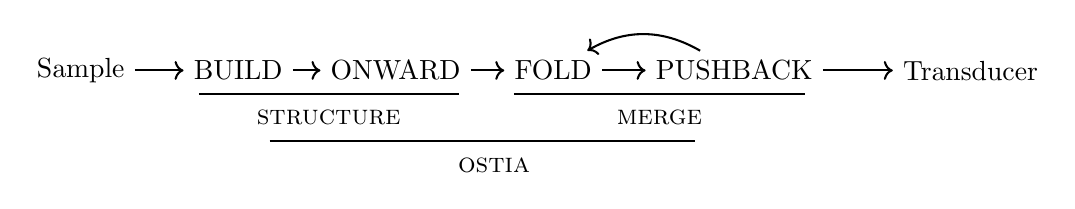
\begin{tikzpicture}
\node[]  at (0, 0) (s) {Sample};
\node[]  at (2, 0) (b) {BUILD};
\node[]  at (4, 0) (o) {ONWARD};
\node[]  at (6, 0) (f) {FOLD};
\node[]  at (8.3, 0) (p) {PUSHBACK};
\node[]  at (11.3, 0) (t) {Transducer};
\path[->]   (s) edge (b)
			(b) edge (o)
			(o) edge (f)
			(f) edge (p)
			(p) edge (t)
			(p) edge[bend right] (f);
\draw[thick] (1.5, -0.3) -- (4.8, -0.3);
\draw[thick] (5.5, -0.3) -- (9.2, -0.3);
\node[]  at (3.15, -0.6) {\textsc{structure}};
\node[]  at (7.35, -0.6) {\textsc{merge}};
\draw[thick] (2.4, -0.9) -- (7.8, -0.9);
\node[]  at (5.25, -1.2) {\textsc{ostia}};
\end{tikzpicture}
\caption{The main steps of OSTIA: \textsc{build}, \textsc{onward}, \textsc{fold} and \textsc{pushback}.}
\label{ostiamainsteps}
\end{figure}



\paragraph{BUILD}

The first step is to represent the input data using a transducer-like data structure.
For this purpose, we can build a \emph{prefix-tree transducer} that reads input strings of the training sample symbol-by-symbol, with the common prefixes of those strings stored in the states.
The initial state $q_\epsilon$ of such a PTT refers to the only common prefix of all the input strings: $\epsilon$.
The names of the later states refer to the common prefix those strings are sharing: the states accessible from the state $q_\epsilon$ correspond to different first symbols of the input strings.
So, for example, a state $q_{aba}$ reads a prefix \emph{aba} by passing through the following states: $q_\epsilon$, $q_{a}$, $q_{ab}$, and $q_{aba}$.
State outputs are set to the translations of the input strings that end up in that state.
For example, given the input pair $(ab, 01)$, we save $01$ in the state output of the state $q_{ab}$.

If the state output is not known, it is marked as $\perp$, or \emph{unknown}.
The unknown state output has two properties: \emph{absorbency} and \emph{neutrality}.
It is absorbent since its concatenation with any other string returns the same ``unknown'' output $\perp$.
It is neutral because the longest common prefix of any set of strings $W$ and $\perp$ is the same as the one of $W$ by itself, i.e.\  $\perp$ is transparent for this operation.
In such a way, the training sample provided to OSTIA is represented as a PTT.


\paragraph{ONWARD}

The outputs of the PTT are then modified to be \emph{onward}: such a PTT outputs translations as early as possible.
During this step, common prefixes of state outputs are pushed closer to the initial state.
For example, assume that the intermediate state of the PTT is the one as pictured in \ref{onwardgfsts} on the left side, with the onward version of that PTT on the right side.
In the input PPT, the state output of the state $q_a$ is $1$, and the translations on all edges coming out of $q_a$ ($q_a\xrightarrow{\text{a:10}}q_{aa}$ and $q_a\xrightarrow{\text{b:11}}q_{ab}$) also contain $1$ as their prefix.
Therefore, this prefix can be removed from the state output and transitions, and be introduced in the transducer earlier, namely, on the transition incoming into the state $q_a$.
Onwarding starts from the \emph{leaves} of the PTT (the nodes that do not have any outcoming arcs), and percolates to the initial state $q_\epsilon$.




\begin{figure}[h!] 
\centering
\begin{tikzpicture}
\node[state, initial]  at (0,1) (e) {$\epsilon:\epsilon$};
\node[state]  at (2,1) (a) {a:1};
\node[state]  at (4,2) (aa) {aa:$\epsilon$};
\node[state]  at (4,0) (ab) {ab:$\epsilon$};
\path[->] (e) edge[above] node{a:$\epsilon$} (a)
		  (a) edge[above] node{a:10} (aa)
		  (a) edge[above] node{b:11} (ab);
\end{tikzpicture}
%
\hspace{3em}
%
\begin{tikzpicture}
\node[state, initial]  at (0,1) (e) {$\epsilon:\epsilon$};
\node[state]  at (2,1) (a) {a:$\epsilon$};
\node[state]  at (4,2) (aa) {aa:$\epsilon$};
\node[state]  at (4,0) (ab) {ab:$\epsilon$};
\path[->] (e) edge[above] node{a:1} (a)
		  (a) edge[above] node{a:0} (aa)
		  (a) edge[above] node{b:1} (ab);
\end{tikzpicture}
\caption{Non-onward and onward PTTs that are otherwise equivalent.}
\label{onwardgfsts}
\end{figure}



\paragraph{FOLD}

Then, we try to merge every pair of states of the PTT.
If (a) the state outputs of $q$ and $q'$ are the same or are $\perp$, (b) all the incoming branches of $q'$ can be redirected to $q$, and (c) all outgoing branches from $q'$ are consistent with the outgoing branches of $q$, states $q$ and $q'$ are merged.
Consistency implies either having matching outgoing branches, a possibility to add a missing branch, or, if required, being able to successfully delay a part of the output during the \emph{pushback} step.
Folding one state into another decreases the size of the transducer, and shows that the learner generalized the pattern.


\paragraph{PUSHBACK}

The pushback operation checks if a part of the output can be delayed and therefore removed from some transitions.
If pushing back a portion of the output is possible, states $q$ and $q'$ considered during the previous \emph{merge} step are combined, otherwise, their merge is rejected.
For example, consider the FST on the left side in figure \ref{pushbackostia}.
Reading \emph{a} from the state $q_\epsilon$ yields the translation \emph{uv}.
However, as the machine on the right shows, the translation's suffix \emph{v} can be delayed to the state output of $q_a$ and all the transitions outgoing from $q_a$.
It could let the state $q_e$ be merged with some other state in the FST.
After the pushback, OSTIA returns to the merging step and checks if there are other pairs of states that could be merged.
When no such pairs remain, OSTIA outputs the FST.
In some sense, \emph{pushback} is the operation opposite to \emph{onward} since it delays the outputs, but the resulting FST is always onward.

\begin{figure}[h!] 
\centering
\begin{tikzpicture}
\node[state, initial]  at (0,1) (e) {$\epsilon:\epsilon$};
\node[state]  at (2,1) (a) {a:$\epsilon$};
\node[state]  at (4,2) (aa) {aa:$\epsilon$};
\node[state]  at (4,0) (ab) {ab:$\epsilon$};
\path[->] (e) edge[above] node{a:uv} (a)
		  (a) edge[above] node{a:$\epsilon$} (aa)
		  (a) edge[above] node{b:$\epsilon$} (ab);
\end{tikzpicture}
%
\hspace{3em}
%
\begin{tikzpicture}
\node[state, initial]  at (0,1) (e) {$\epsilon:\epsilon$};
\node[state]  at (2,1) (a) {a:v};
\node[state]  at (4,2) (aa) {aa:$\epsilon$};
\node[state]  at (4,0) (ab) {ab:$\epsilon$};
\path[->] (e) edge[above] node{a:u} (a)
		  (a) edge[above] node{a:v} (aa)
		  (a) edge[above] node{b:v} (ab);
\end{tikzpicture}
\caption{OSTIA pushes back the suffix \emph{v}.}
\label{pushbackostia}
\end{figure}


In such a way, OSTIA constructs a subsequential FST that generalizes the mapping from the input strings into their output representations.
Note, that as well as the subregular learning algorithms discussed earlier in Chapter $3$, OSTIA requires a sample of only positive data.%
\footnote{The algorithmic complexity of OSTIA is $\mathcal{O}(n^3(m + \mid\Sigma\mid) + nm\mid\Sigma\mid)$, where $n$ is the sum of the input string lengths, $m$ is the length of the longest output string, and $\Sigma$ is the input alphabet \citep{DeLaHiguera2010}.}
The next subsection presents the inference steps of this algorithm given a concrete example.



\subsection{The successful example}
\label{exam1}

Here, I discuss a slightly modified example of the OSTIA inference steps originally presented in \cite{DeLaHiguera2010}.
The task is to learn the following mapping: word-final $a$ is rewritten as $1$, non-word-final $a$ corresponds to $0$, and $b$ is always translated as $1$.
Notice, that this pattern can be viewed as a generalization of a linguistically-motivated process of word-final devoicing since it involves a segment changing its value to the opposite at the end of the word.
The training sample that I use in this example is enlarged in comparison to the one presented by \cite{DeLaHiguera2010}: it provides \emph{all} the necessary pairs that guarantee the extraction of the pattern.

\textbf{Sample} = {[}(b, 1), (a, 1), (aa, 01), (ab, 01), (aba, 011), (aaa, 001){]}


\paragraph{Step I.}

At first, OSTIA constructs a PTT representing the input sample.
This PTT reads the left sides of the training sample one symbol at a time.
For every string $w$ of the input pair ($w$, $o$), there exists a state $q_w$ with the state output $o$.
All transitions of this PTT output an empty string.
If there is a state $q_{w'}$ that does not correspond to any input string of the training sample, its state output is $\perp$.
For example, there is no empty string in the given sample, so the state output of $q_\epsilon$ is $\perp$.

%\begin{figure}[h!] 
%\centering
\begin{center}
\begin{tikzpicture}
\small
\node[state, initial]  at (0,0) (e) {$\epsilon:\perp$};
\node[state]  at (2,1) (a) {a:1};
\node[state]  at (2,-1) (b) {b:1};
\node[state]  at (4,2) (aa) {aa:01};
\node[state]  at (6,2) (aaa) {aaa:001};
\node[state]  at (4,0) (ab) {ab:01};
\node[state]  at (6,0) (aba) {aba:011};
\path[->] (e) edge[above] node{a:$\epsilon$} (a)
		  (e) edge[above] node{b:$\epsilon$} (b)
		  (a) edge[above] node{a:$\epsilon$} (aa)
		  (a) edge[above] node{b:$\epsilon$} (ab)
		  (aa) edge[above] node{a:$\epsilon$} (aaa)
		  (ab) edge[above] node{a:$\epsilon$} (aba);
\end{tikzpicture}
\end{center}
%\caption{After step I: constructing the PTT}
%\label{ostiastep1}
%\end{figure}

\paragraph{Step II.}

Then, this PTT is onwarded.
For example, consider the state $q_{aaa}$ with the state output $001$.
We can replace it by $\epsilon$, and instead move $001$ to the incoming arc therefore obtaining a transition $q_{aa}\xrightarrow{\text{a:001}}q_{aaa}$.
The longest common prefix of the modified transition and the state output of $q_{aa}$ is the longest common prefix of $01$ and $001$, and that $0$ can be moved to the output of the arc $q_{a}\xrightarrow{\text{a:0}}q_{aa}$.
Other leaves of the FST are processed similarly.
After this step, the input sample is represented as an onward PTT.

\begin{center}
\begin{tikzpicture}
\small
\node[state, initial]  at (0,0) (e) {$\epsilon:\perp$};
\node[state]  at (2,1) (a) {a:1};
\node[state]  at (2,-1) (b) {b:$\epsilon$};
\node[state]  at (4,2) (aa) {aa:1};
\node[state]  at (6,2) (aaa) {aaa:$\epsilon$};
\node[state]  at (4,0) (ab) {ab:$\epsilon$};
\node[state]  at (6,0) (aba) {aba:$\epsilon$};
\path[->] (e) edge[above] node{a:$\epsilon$} (a)
		  (e) edge[above] node{b:1} (b)
		  (a) edge[above] node{a:0} (aa)
		  (a) edge[above] node{b:01} (ab)
		  (aa) edge[above] node{a:01} (aaa)
		  (ab) edge[above] node{a:1} (aba);
\end{tikzpicture}
\end{center}

\paragraph{Step III.}

Next, we start the process of generalizing the obtained PTT by trying to merge pairs of its states.
States are colored in two colors: red and blue.
\emph{Red states} cannot be eliminated from the FST: they are crucial and therefore cannot be folded into any other state.
At first, only the initial state $q_\epsilon$ is colored red.
All states that can be reached in one step from the red states are colored blue.
The status of \emph{blue states} is unclear: either they will be folded into some red states, or they will eventually be re-colored red.
After a state was colored red, its immediate children are automatically added to the list of blue states.
In our example, two states are colored blue -- $q_a$ and $q_b$ -- since they can be reached from $q_\epsilon$ in one step.


%\begin{figure}[h!] 
%\centering
\begin{center}
\begin{tikzpicture}
\small
\node[state, initial, red]  at (0,0) (e) {$\epsilon:\perp$};
\node[state, blue]  at (2,1) (a) {a:1};
\node[state, blue]  at (2,-1) (b) {b:$\epsilon$};
\node[state]  at (4,2) (aa) {aa:1};
\node[state]  at (6,2) (aaa) {aaa:$\epsilon$};
\node[state]  at (4,0) (ab) {ab:$\epsilon$};
\node[state]  at (6,0) (aba) {aba:$\epsilon$};
\path[->] (e) edge[above] node{a:$\epsilon$} (a)
		  (e) edge[above] node{b:1} (b)
		  (a) edge[above] node{a:0} (aa)
		  (a) edge[above] node{b:01} (ab)
		  (aa) edge[above] node{a:01} (aaa)
		  (ab) edge[above] node{a:1} (aba);
\end{tikzpicture}
\end{center}
%\caption{After steps II and III: onwarding the PTT and coloring the states}
%\label{ostiastep23}
%\end{figure}

\paragraph{Step IV.}

Then, the algorithm considers pairs where one state is red and another one is blue and tries to fold the blue state into the red one.
Let us then fold the state $q_b$ into $q_\epsilon$.
At first, we check if the state outputs of $q_b$ and $q_\epsilon$ are compatible.
They are $\perp$ and $\epsilon$, and therefore could be merged: they are \emph{not different} due to the transparency of $\perp$, so we assign $\epsilon$ to the state output of $q_\epsilon$.
The transition coming to the state $q_b$ is re-directed into the state $q_\epsilon$ thus yielding a loop on that state.
There is no other sub-tree rooted in $q_b$, so folding $q_b$ into $q_\epsilon$ can be finalized, and $q_b$ is removed from the FST.

\begin{center}
\begin{tikzpicture}
\small
\node[state, initial, red]  at (0,1) (e) {$\epsilon:\epsilon$};
\node[state, blue]  at (2,1) (a) {a:1};
\node[state]  at (4,2) (aa) {aa:1};
\node[state]  at (6,2) (aaa) {aaa:$\epsilon$};
\node[state]  at (4,0) (ab) {ab:$\epsilon$};
\node[state]  at (6,0) (aba) {aba:$\epsilon$};
\path[->] (e) edge[above] node{a:$\epsilon$} (a)
		  (e) edge[loop above] node{b:1} (e)
		  (a) edge[above] node{a:0} (aa)
		  (a) edge[above] node{b:01} (ab)
		  (aa) edge[above] node{a:01} (aaa)
		  (ab) edge[above] node{a:1} (aba);
\end{tikzpicture}
\end{center}

\paragraph{Step V.}

After the state $q_b$ is eliminated, $q_a$ is the only blue state left.
We therefore consider merging $q_a$ into $q_\epsilon$.
However, these two states have different state outputs, and therefore it is impossible.
As the result, $q_a$ is re-colored red, and $q_{aa}$ and $q_{ab}$ accessible in one step from $q_a$ are colored blue.


%\begin{figure}[h!] 
%\centering
\begin{center}
\begin{tikzpicture}
\small
\node[state, initial, red]  at (0,1) (e) {$\epsilon:\epsilon$};
\node[state, red]  at (2,1) (a) {a:1};
\node[state, blue]  at (4,2) (aa) {aa:1};
\node[state]  at (6,2) (aaa) {aaa:$\epsilon$};
\node[state, blue]  at (4,0) (ab) {ab:$\epsilon$};
\node[state]  at (6,0) (aba) {aba:$\epsilon$};
\path[->] (e) edge[above] node{a:$\epsilon$} (a)
		  (e) edge[loop above] node{b:1} (e)
		  (a) edge[above] node{a:0} (aa)
		  (a) edge[above] node{b:01} (ab)
		  (aa) edge[above] node{a:01} (aaa)
		  (ab) edge[above] node{a:1} (aba);
\end{tikzpicture}
\end{center}
%\caption{After steps IV and V: folded $q_b$ into $q_\epsilon$ and re-colored the states}
%\label{ostiastep45}
%\end{figure}

\paragraph{Step VI.}

We then try to merge $q_\epsilon$ and $q_{aa}$, but it is not possible since they have different state outputs.
States $q_{a}$ and $q_{aa}$ could be merged because they have the same state output: $1$.
The outgoing arcs reading $a$ from these two states are different: one outputs $0$, and another outputs $01$.
However, the difference is the suffix $1$ that can be pushed further to the state output of $q_{aaa}$, therefore making those two transitions identical.
The arrow incoming to $q_{aa}$ is then re-directed to $q_{a}$, and $q_{aa}$ is eliminated from the list of states.

%\begin{figure}[h!] 
%\centering
\begin{center}
\begin{tikzpicture}
\small
\node[state, initial, red]  at (0,1) (e) {$\epsilon:\epsilon$};
\node[state, red]  at (2,1) (a) {a:1};
%\node[state, blue]  at (4,2) (aa) {aa:1};
\node[state]  at (6,2) (aaa) {aaa:1};
\node[state, blue]  at (4,0) (ab) {ab:$\epsilon$};
\node[state]  at (6,0) (aba) {aba:$\epsilon$};
\path[->] (e) edge[above] node{a:$\epsilon$} (a)
		  (e) edge[loop above] node{b:1} (e)
		  (a) edge[loop above] node{a:0} (a)
		  (a) edge[above] node{b:01} (ab)
%		  (aa) edge[above] node{a:01} (aaa)
		  (ab) edge[above] node{a:1} (aba);
\end{tikzpicture}
\end{center}
%\caption{After step VI: folded $q_{aa}$ into $q_{a}$}
%\label{ostiastep6}
%\end{figure}


\paragraph{Step VII.}

The state $q_{ab}$ is then folded into $q_{\epsilon}$.
The incoming arrow is re-directed to $q_{\epsilon}$, and $1$ is pushed back to state state output of $q_{aba}$.
Since $q_{ab}$ was merged with another state, it is eliminated from the machine.
This leaves no other blue states in the machine, and it signifies that OSTIA completed the inference.

%\begin{figure}[h!] 
%\centering
\begin{center}
\begin{tikzpicture}
\small
\node[state, initial, red]  at (0,1) (e) {$\epsilon:\epsilon$};
\node[state, red]  at (3,1) (a) {a:1};
\node[state]  at (6,2) (aaa) {aaa:1};
\node[state]  at (6,0) (aba) {aba:1};
\path[->] (e) edge[above,, bend left] node{a:$\epsilon$} (a)
		  (e) edge[loop above] node{b:1} (e)
		  (a) edge[loop above] node{a:0} (a)
		  (a) edge[above, bend left] node{b:01} (e);
\end{tikzpicture}
\end{center}
%\caption{After step VII: folded $q_{ab}$ into $q_{\epsilon}$}
%\label{ostiastep7}
%\end{figure}

\paragraph{Step VIII.}

All blue states are now eliminated from the machine.
However, the states that were never colored are still present.
In SigmaPie, the last step included in the \emph{OSTIA} algorithm is the elimination of the unaccessible states from the machine.
After those steps are completed, we obtain the FST visualized below.% in \ref{ostialaststep}.

%\begin{figure}[h!] 
%\centering
\begin{center}
\begin{tikzpicture}
\small
\node[state, initial]  at (0,0) (e) {$\epsilon:\epsilon$};
\node[state] at (3,0) (a) {a:1};
\path[->] (e) edge[loop above] node{b:1} (e)
	(e) edge[above, bend left] node{a:$\epsilon$} (a)
	(a) edge[below, bend left] node{b:01} (e)
	(a) edge[loop above] node{a:0} (a);
\end{tikzpicture}
\end{center}
%\caption{OSTIA: the resulting FST}
%\label{ostialaststep}
%\end{figure}


\subsection{The unsuccessful example}
\label{exam2}

Now, consider a pattern of \emph{unbounded tone plateauing} (UTP).
In a pattern like that, a sequence of low tones is converted to high if surrounded by high tones.
For example, inputs \emph{HLH} and \emph{HLLLH} are mapped to the outputs \emph{HHH} and \emph{HHHHH}, correspondingly.
When a low tone $L$ follows a high tone, it might be written as either $L$ or $H$ depending on the presence of another $H$ anywhere further in the input.
In other words, it requires an \emph{unbounded lookahead}.

Patterns requiring lookahead, such as UTP, are called \emph{unbounded circumambient processes} since the triggers are located on both sides of the undergoer, and they can be arbitrary far from it.
Unbounded circumambient processes are not subsequential \citep{Jardine2016}, and therefore it is expected that OSTIA is unable to capture UTP.
I show that OSTIA fails to learn UTP with the following sample.

\textbf{Sample} = {[}(HHH, HHH), (HHL, HHL), (HL, HL), (HLH, HHH), (HLL, HLL), (HLLH, HHHH){]}

\paragraph{Step I.}
At first, consider a PTT corresponding to the given training sample $S$.

\begin{center}
\begin{tikzpicture}
\small
\node[state, initial]  at (0,0) (e) {$\epsilon:\perp$};
\node[state]  at (2,0) (H) {H:$\perp$};
\node[state]  at (4,2.3) (HH) {HH:$\perp$};
\node[state]  at (7,3.5) (HHH) {HHH:HHH};
\node[state]  at (7,1.1) (HHL) {HHL:HHL};
\node[state]  at (4,-2.3) (HL) {HL:HL};
\node[state]  at (7,-1.1) (HLH) {HLH:HHH};
\node[state]  at (7,-3.5) (HLL) {HLL:HLL};
\node[state]  at (10,-3.5) (HLLH) {HLLH:HLLH};
\path[->] (e) edge[above] node{H:$\epsilon$} (H)
		(H) edge[left] node{H:$\epsilon$} (HH)
		(H) edge[left] node{L:$\epsilon$} (HL)
		(HH) edge[above] node{H:$\epsilon$} (HHH)
		(HH) edge[above] node{L:$\epsilon$} (HHL)
		(HL) edge[above] node{H:$\epsilon$} (HLH)
		(HL) edge[above] node{L:$\epsilon$} (HLL)
		(HLL) edge[above] node{H:$\epsilon$} (HLLH);
\end{tikzpicture}
\end{center}

\paragraph{Step II.}
Then, as previously, let us push the state outputs from the leaf nodes closer to the initial state $q_\epsilon$.
The resulting PTT is onward.

\begin{center}
\begin{tikzpicture}
\small
\node[state, initial]  at (0,0.25) (e) {$\epsilon:\perp$};
\node[state]  at (2,0.25) (H) {H:$\perp$};
\node[state]  at (4,1.9) (HH) {HH:$\perp$};
\node[state]  at (7,2.7) (HHH) {HHH:$\epsilon$};
\node[state]  at (7,1.1) (HHL) {HHL:$\epsilon$};
\node[state]  at (4,-1.4) (HL) {HL:L};
\node[state]  at (7,-0.6) (HLH) {HLH:$\epsilon$};
\node[state]  at (7,-2.2) (HLL) {HLL:LL};
\node[state]  at (10,-2.2) (HLLH) {HLLH:$\epsilon$};
\path[->] (e) edge[above] node{H:H} (H)
		(H) edge[left] node{H:H} (HH)
		(H) edge[left] node{L:$\epsilon$} (HL)
		(HH) edge[above] node{H:H} (HHH)
		(HH) edge[above] node{L:L} (HHL)
		(HL) edge[above] node{H:HH} (HLH)
		(HL) edge[above] node{L:$\epsilon$} (HLL)
		(HLL) edge[above] node{H:HHH} (HLLH);
\end{tikzpicture}
\end{center}

\paragraph{Step III.}

Next, we prepare to start folding states and sub-trees of the PTT into each other by coloring the states in red and blue.
As previously, the initial state $q_\epsilon$ is colored red, and the state $q_H$ available from $q_\epsilon$ in one step is colored blue.

\begin{center}
\begin{tikzpicture}
\small
\node[state, initial, red]  at (0,0.25) (e) {$\epsilon:\perp$};
\node[state, blue]  at (2,0.25) (H) {H:$\perp$};
\node[state]  at (4,1.9) (HH) {HH:$\perp$};
\node[state]  at (7,2.7) (HHH) {HHH:$\epsilon$};
\node[state]  at (7,1.1) (HHL) {HHL:$\epsilon$};
\node[state]  at (4,-1.4) (HL) {HL:L};
\node[state]  at (7,-0.6) (HLH) {HLH:$\epsilon$};
\node[state]  at (7,-2.2) (HLL) {HLL:LL};
\node[state]  at (10,-2.2) (HLLH) {HLLH:$\epsilon$};
\path[->] (e) edge[above] node{H:H} (H)
		(H) edge[left] node{H:H} (HH)
		(H) edge[left] node{L:$\epsilon$} (HL)
		(HH) edge[above] node{H:H} (HHH)
		(HH) edge[above] node{L:L} (HHL)
		(HL) edge[above] node{H:HH} (HLH)
		(HL) edge[above] node{L:$\epsilon$} (HLL)
		(HLL) edge[above] node{H:HHH} (HLLH);
\end{tikzpicture}
\end{center}

\paragraph{Step IV.}

The algorithm attempts to merge the blue state into the red state.
However, it is not possible to fold the sub-tree of $q_H$ into $q_\epsilon$.
It would cause the arrow $q_{HH}\xrightarrow{\text{L:L}}q_{HHL}$ to be changed to $q_{\epsilon}\xrightarrow{\text{L:L}}q_{HHL}$.
It means that states $q_{HHL}$ and $q_{HL}$ need to be merged since both of them would be available from $q_\epsilon$ by reading $L$, but it is not possible because the state outputs of $q_{HHL}$ and $q_{HL}$ are different: \emph{$\epsilon$} and \emph{L}, correspondingly.
Therefore the merge is rejected, and $q_H$ is colored red.
Its daughter nodes $q_{HH}$ and $q_{HL}$ are now blue.

\begin{center}
\begin{tikzpicture}
\small
\node[state, initial, red]  at (0,0.25) (e) {$\epsilon:\perp$};
\node[state, red]  at (2,0.25) (H) {H:$\perp$};
\node[state, blue]  at (4,1.9) (HH) {HH:$\perp$};
\node[state]  at (7,2.7) (HHH) {HHH:$\epsilon$};
\node[state]  at (7,1.1) (HHL) {HHL:$\epsilon$};
\node[state, blue]  at (4,-1.4) (HL) {HL:L};
\node[state]  at (7,-0.6) (HLH) {HLH:$\epsilon$};
\node[state]  at (7,-2.2) (HLL) {HLL:LL};
\node[state]  at (10,-2.2) (HLLH) {HLLH:$\epsilon$};
\path[->] (e) edge[above] node{H:H} (H)
		(H) edge[left] node{H:H} (HH)
		(H) edge[left] node{L:$\epsilon$} (HL)
		(HH) edge[above] node{H:H} (HHH)
		(HH) edge[above] node{L:L} (HHL)
		(HL) edge[above] node{H:HH} (HLH)
		(HL) edge[above] node{L:$\epsilon$} (HLL)
		(HLL) edge[above] node{H:HHH} (HLLH);
\end{tikzpicture}
\end{center}

\paragraph{Step V.}

The state $q_{HH}$ can be merged with $q_\epsilon$.
Indeed, the outgoing arcs reading and writing $H$ are present in both of these states, and the outgoing arc from $q_{HH}$ to $q_{HHL}$ is now re-directed and originates from $q_{\epsilon}$.
All the incoming arcs into the state $q_{HH}$ are re-directed to target $q_\epsilon$.
It created two outgoing from the state $q_\epsilon$ arrows reading $H$: $q_{\epsilon}\xrightarrow{\text{H:H}}q_{H}$ and $q_{\epsilon}\xrightarrow{\text{H:H}}q_{HHH}$, so $q_{HHH}$ needed to be folded into $q_{H}$.
Their state outputs are compatible since they are $\perp$ and $\epsilon$, therefore, the output of the state $q_{H}$ was rewritten to $\epsilon$.


\begin{center}
\begin{tikzpicture}
\small
\node[state, initial, red]  at (0,0) (e) {$\epsilon:\perp$};
\node[state, red]  at (2,0) (H) {H:$\epsilon$};
\node[state]  at (1.3,1.9) (HHL) {HHL:$\epsilon$};
\node[state, blue]  at (4,0) (HL) {HL:L};
\node[state]  at (7,0.8) (HLH) {HLH:$\epsilon$};
\node[state]  at (7,-0.8) (HLL) {HLL:LL};
\node[state]  at (10,-0.8) (HLLH) {HLLH:$\epsilon$};
\path[->] (e) edge[above, bend left] node{H:H} (H)
		(H) edge[below, bend left] node{H:$\epsilon$} (e)
		(H) edge[above] node{L:$\epsilon$} (HL)
		(e) edge[left] node{L:L} (HHL)
		(HL) edge[above] node{H:HH} (HLH)
		(HL) edge[above] node{L:$\epsilon$} (HLL)
		(HLL) edge[above] node{H:HHH} (HLLH);
\end{tikzpicture}
\end{center}

\paragraph{Step VI.}

The state $q_{HL}$ can be merged with neither $q_\epsilon$ nor $q_{H}$ because the arrows reading $L$ bring the machine to states with different state outputs.
While the state output of $q_{HLL}$ is $LL$, $q_{HL}$ and $q_{HHL}$ output $L$ and $\epsilon$, correspondingly.
Therefore $q_{HL}$ is colored red, and its children $q_{HLH}$ and $q_{HLL}$ are now blue.
Additionally, $q_{HHL}$ is also blue because it originates from the red state $q_\epsilon$.


\begin{center}
\begin{tikzpicture}
\small
\node[state, initial, red]  at (0,0) (e) {$\epsilon:\perp$};
\node[state, red]  at (2,0) (H) {H:$\epsilon$};
\node[state, blue]  at (1.3,1.9) (HHL) {HHL:$\epsilon$};
\node[state, red]  at (4,0) (HL) {HL:L};
\node[state, blue]  at (7,0.8) (HLH) {HLH:$\epsilon$};
\node[state, blue]  at (7,-0.8) (HLL) {HLL:LL};
\node[state]  at (10,-0.8) (HLLH) {HLLH:$\epsilon$};
\path[->] (e) edge[above, bend left] node{H:H} (H)
		(H) edge[below, bend left] node{H:$\epsilon$} (e)
		(H) edge[above] node{L:$\epsilon$} (HL)
		(e) edge[left] node{L:L} (HHL)
		(HL) edge[above] node{H:HH} (HLH)
		(HL) edge[above] node{L:$\epsilon$} (HLL)
		(HLL) edge[above] node{H:HHH} (HLLH);
\end{tikzpicture}
\end{center}

\paragraph{Step VII.}

The state $q_{HLH}$ is merged with $q_\epsilon$, and the only arrow incoming in $q_{HLH}$ from $q_{HL}$ is now targeting $q_\epsilon$.
Since the state output of $q_{HLH}$ was $\epsilon$ and the one of $q_\epsilon$ was unknown, it is now re-defined as $\epsilon$.

\begin{center}
\begin{tikzpicture}
\small
\node[state, initial, red]  at (0,0) (e) {$\epsilon:\epsilon$};
\node[state, red]  at (2,0) (H) {H:$\epsilon$};
\node[state, blue]  at (1.3,1.9) (HHL) {HHL:$\epsilon$};
\node[state, red]  at (4,0) (HL) {HL:L};
\node[state, blue]  at (6,0) (HLL) {HLL:LL};
\node[state]  at (9,0) (HLLH) {HLLH:$\epsilon$};
\path[->] (e) edge[above, bend left] node{H:H} (H)
		(H) edge[below, bend left] node{H:$\epsilon$} (e)
		(H) edge[above] node{L:$\epsilon$} (HL)
		(e) edge[left] node{L:L} (HHL)
		(HL) edge[above, bend left=60] node{H:HH} (e)
		(HL) edge[above] node{L:$\epsilon$} (HLL)
		(HLL) edge[above] node{H:HHH} (HLLH);
\end{tikzpicture}
\end{center}

\paragraph{Step VIII.}

The state $q_{HLL}$ cannot be merged with any red state.
Its state output differs from those of all the red states.
The state $q_{HLL}$ is thus colored red, and its daughter state $q_{HLLH}$ is blue.

\begin{center}
\begin{tikzpicture}
\small
\node[state, initial, red]  at (0,0) (e) {$\epsilon:\epsilon$};
\node[state, red]  at (2,0) (H) {H:$\epsilon$};
\node[state, blue]  at (1.3,1.9) (HHL) {HHL:$\epsilon$};
\node[state, red]  at (4,0) (HL) {HL:L};
\node[state, red]  at (6,0) (HLL) {HLL:LL};
\node[state, blue]  at (9,0) (HLLH) {HLLH:$\epsilon$};
\path[->] (e) edge[above, bend left] node{H:H} (H)
		(H) edge[below, bend left] node{H:$\epsilon$} (e)
		(H) edge[above] node{L:$\epsilon$} (HL)
		(e) edge[left] node{L:L} (HHL)
		(HL) edge[above, bend left=60] node{H:HH} (e)
		(HL) edge[above] node{L:$\epsilon$} (HLL)
		(HLL) edge[above] node{H:HHH} (HLLH);
\end{tikzpicture}
\end{center}

\paragraph{Step IX.}

The state $q_{HLLH}$ is then merged with $q_\epsilon$, and the arrow incoming in it from the state $q_{HLL}$ is re-directed.
At this moment it is already clear that the algorithm failed to learn the UTP pattern.
The learner memorized that one or two $L$ need to be substituted by $H$ if they are followed by $H$, but did not generalize it to an unbounded number of $L$s.

\begin{center}
\begin{tikzpicture}
\small
\node[state, initial, red]  at (0,0) (e) {$\epsilon:\epsilon$};
\node[state, red]  at (2,0) (H) {H:$\epsilon$};
\node[state, blue]  at (1.3,1.9) (HHL) {HHL:$\epsilon$};
\node[state, red]  at (4,0) (HL) {HL:L};
\node[state, red]  at (6,0) (HLL) {HLL:LL};
\path[->] (e) edge[above, bend left] node{H:H} (H)
		(H) edge[below, bend left] node{H:$\epsilon$} (e)
		(H) edge[above] node{L:$\epsilon$} (HL)
		(e) edge[left] node{L:L} (HHL)
		(HL) edge[above, bend left=60] node{H:HH} (e)
		(HL) edge[above] node{L:$\epsilon$} (HLL)
		(HLL) edge[above, bend left=60] node{H:HHH} (e);
\end{tikzpicture}
\end{center}


\paragraph{Step X.}

Finally, the only remaining state $q_{HHL}$ is merged with $q_\epsilon$, therefore, creating a loop that reads and writes $L$ on that state.
There are no other remaining blue states, and therefore the learner outputs the FST.


\begin{center}
\begin{tikzpicture}
\small
\node[state, initial]  at (0,0) (e) {$\epsilon:\epsilon$};
\node[state]  at (2,0) (H) {H:$\epsilon$};
\node[state]  at (4,0) (HL) {HL:L};
\node[state]  at (6,0) (HLL) {HLL:LL};
\path[->] (e) edge[above, bend left] node{H:H} (H)
		(H) edge[below, bend left] node{H:$\epsilon$} (e)
		(H) edge[above] node{L:$\epsilon$} (HL)
		(e) edge[loop above, left] node{L:L} (e)
		(HL) edge[above, bend left=60] node{H:HH} (e)
		(HL) edge[above] node{L:$\epsilon$} (HLL)
		(HLL) edge[above, bend left=60] node{H:HHH} (e);
\end{tikzpicture}
\end{center}

As one can see, this transducer does not represent the UTP pattern.
For example, it would re-write an input string \emph{HLHLH} as \emph{HHHLH} by passing through the following states: $q_{\epsilon}\xrightarrow{\text{H:H}}q_{H}\xrightarrow{\text{L:$\epsilon$}}q_{HL}\xrightarrow{\text{H:HH}}q_{\epsilon}\xrightarrow{\text{L:L}}q_{\epsilon}\xrightarrow{\text{H:H}}q_{H}$.
Indeed, UTP cannot be expressed using a subsequential function: it requires an unbounded lookahead \citep{Jardine2016}.


\section{Learning experiments}
\label{learningexperiments}

Here, I discuss the learning experiments that I used to explore the capacities of the OSTIA algorithm.
Interestingly, OSTIA performed extremely well ($100$\%) on one or more harmonies without blockers.
However, the blocking effect showed itself as a challenge for the learner: the accuracy was falling drastically with the increasing length of the evaluated strings.

In this chapter, in contrast to the previous one, the learner extracts the ``rewrite rules'' instead of acquiring well-formedness conditions.
Namely, the learner is given a pair of strings imitating the underlying representation (UR) and the surface form (SF), and its goal is to learn how to map one into another.
This allows us to explore the capacities of OSTIA when challenged with natural language-like patterns discussed in the previous chapter: single and double harmonic systems with or without blockers, and others.
The code behind the experiments is available on GitHub \href{https://github.com/alenaks/subregular-experiments}{\faGithub} \citep{GHsubex}.

Note, however, the critical importance of the concrete implementation for the results of OSTIA.
For example, the condition activating pushback is slightly different in various OSTIA's pseudocodes.
\cite{OncinaEtAl1993} in the original formulation of OSTIA execute the pushback step depending on the output of $q_a$ transitions being a prefix of the corresponding $q_b$ transitions.
The core architecture of their learner, however, is a bit different from the one described in this section since their learner necessarily annotates the data with the end-markers and uses this information for the inference steps.
\cite{DeLaHiguera2010} executes the pushback and folds the states $q_a$ and $q_b$ if all outgoing transitions from those states carry the same output.
As one can see, in this case, the pushback step would not be useful: if the outputs of the transitions are identical, there is no disagreeing affix to be pushed further in the FST.
In the errata for his book, \cite{DeLaHiguera2011} changes that condition to depend on the color of the states accessible from $q_b$.
The OSTIA version implemented and used in this chapter has its core architecture following \cite{DeLaHiguera2010}, but the condition is in line with \cite{OncinaEtAl1993}.
There is a multitude of different versions of pseudocodes, and, therefore, even more versions of the possible implementations.
Thus the results obtained in this chapter are specific to the concrete interpretation of the fold and pushback conditions and need to be tested with different perspectives as well.


\subsection{Experimental setup}

As before, the experiments include $3$ main steps: \emph{data generation}, \emph{learning}, and \emph{model evaluation}.
%In this case, however, there are no experiments targeting raw natural language data since to the best of my knowledge, there are no such datasets available where underlying representations are mapped to their surface forms.

At first, the training pairs were generated.
For example, assume that we are trying to learn a single vowel harmony without blockers, where vowels are $A = \{a, o\}$, and the only consonant is $x$ that is making this harmony long-distant.
The training sample will then contain pairs such as \emph{(xoxxAxAxxxA, xoxxoxoxxxo)} and \emph{(axAxAxxA, axaxaxxa)}, where $A$ refers to an underspecified harmonizing vowel.
The left side of every pair contains the ``underlying representation'', where only the value of the first vowel is established, and all the consecutive vowels are hidden and represented as the name of their harmonic set, in this case, $A$.
The right side contains the ``surface forms'', where all the vowels harmonize with each other.
Such training pairs were then fed to OSTIA that outputted an FST representing the pattern. 

To evaluate the performance of the obtained FST, following \cite{GildeaJurafsky1996}, I generated another set of pairs that are used as a testing sample.
I provided the left-hand sides of those pairs to the FST as input and observed if the output strings were the same as the right-hand sides of the testing sample.

I used two types of testing samples: one includes strings of the same length as the ones that were used for training, and the second one contains strings that are twice longer than the latter.
The test sets containing a longer strings helped me to explore how well OSTIA generalized the target pattern beyond memorization of the concrete shapes found in the training sample.


\subsection{Target patterns}

Among the patterns that I targeted while exploring the capacities of the learner, there were some local patterns such as word-final devoicing, different types of long-distance harmonies, and some circumambient and unattested patterns.
Below I explain the parameters that I considered when choosing the learning experiments, see the summary in figure \ref{typesofexperiments}.

\paragraph{Long-distance}
The difference between local and long-distance processes is one of the very important distinctions for phonology.
In the first case, the process is locally bounded, whereas, in the second one, it involves a potentially unbounded amount of the intervening material.
As I show in chapter 3, this difference is crucial for strictly local models.
They can evaluate local dependencies, but cannot capture long-distant ones.
As an example of a purely local process, I use the phenomenon of word-final devoicing.

\paragraph{Includes blockers}
The blocking effect is widely discussed in the phonological literature.
Harmony systems with and without blockers cannot always be modeled in the same way.
For example, in chapter 3, I show that strictly piecewise models can express multiple well-formedness conditions, but they cannot capture even simple cases of blocking effects.
In the sample of explored datasets, $3$ out of the $7$ employed harmonies involve blockers.

\paragraph{Multiple processes}
A model cannot always handle multiple processes at the same time.
For example, a single tier-based strictly local grammar can express a vowel or a consonant harmony, but it cannot capture both of them at the same time.
There are a total of $4$ harmonies that involve several harmonic spreadings, and $2$ of them exhibit a blocking effect.


\paragraph{Different undergoers}
Some models can express several spreadings at once if all the harmonizing features are spread among the same sets of elements.
For example, the only case when a tier-based strictly local grammar can capture the agreement in two features is when both features are affecting vowels.
Therefore, $2$ of the explored datasets present this type of a harmonic system, with and without a blocking effect.

\paragraph{Unbounded lookahead}
In subsection \ref{exam2}, I showed that processes that require an unbounded lookahead are not subsequential, and therefore cannot be learned by OSTIA.
Therefore, I use $2$ automatically generated datasets that exhibit circumambient patterns, and show that they cannot be learned by a subsequential learner.

\paragraph{Typologically attested}
Finally, I explore both typologically attested and unattested patterns.
All types of harmonic processes are indeed attested in natural languages, as well as the unbounded tone plateauing.
As an example of a typologically unattested pattern, I use the first-last harmony enforcing the agreement among the initial and the final vowels.
Two datasets are exhibiting the first-last harmony: one of them includes an unbounded lookahead, and the other one does not.


\begin{table}[h]
\centering
\scalebox{0.78}{%
\begin{tabular}{|c|c|c|c|c|c|}
\hline
\textbf{\begin{tabular}[c]{@{}c@{}}long-\\ distant\end{tabular}} & \textbf{\begin{tabular}[c]{@{}c@{}}includes\\ blockers\end{tabular}} & \textbf{\begin{tabular}[c]{@{}c@{}}multiple\\ processes\end{tabular}} & \textbf{\begin{tabular}[c]{@{}c@{}}different\\ undergoers\end{tabular}} & \textbf{\begin{tabular}[c]{@{}c@{}}unbounded\\ lookahead\end{tabular}} & 
\textbf{\begin{tabular}[c]{@{}c@{}}typologically\\ attested\end{tabular}} \\ \hline
\multicolumn{6}{|c|}{\large \textit{word-final devoicing}}    \\ \hline
\cellcolor{gray!50}\faTimes                                                               & \cellcolor{gray!50}\faTimes &  \cellcolor{gray!50}                                                                    \faTimes & \cellcolor{gray!50}\faTimes                                                                        &       \cellcolor{gray!50}\faTimes  & {\Large\faCheck}                                                                 \\ \hline
\multicolumn{6}{|c|}{\large \textit{a single vowel harmony without blocking}}                                                                                                                                                                                        \\ \hline
{\Large\faCheck}  & \cellcolor{gray!50}\faTimes & \cellcolor{gray!50}\faTimes                                                                       &   \cellcolor{gray!50}\faTimes                                                                      &         \cellcolor{gray!50}\faTimes  & {\Large\faCheck}                                                               \\ \hline
\multicolumn{6}{|c|}{\large \textit{a single vowel harmony with blocking}}                                                                                                                                                                                           \\ \hline
{\Large\faCheck} & {\Large\faCheck} & \cellcolor{gray!50}\faTimes                                                                       &     \cellcolor{gray!50}\faTimes                                                                    &         \cellcolor{gray!50}\faTimes  & {\Large\faCheck}                                                               \\ \hline
\multicolumn{6}{|c|}{\large \textit{several vowel harmonies without blocking}}                                                                                                                                                                                       \\ \hline
{\Large\faCheck} &  \cellcolor{gray!50}\faTimes & {\Large\faCheck}                                                                       &        \cellcolor{gray!50}\faTimes                                                                 &          \cellcolor{gray!50}\faTimes  & {\Large\faCheck}                                                              \\ \hline
\multicolumn{6}{|c|}{\large \textit{several vowel harmonies with blocking}}                                                                                                                                                                                          \\ \hline
{\Large\faCheck} &  {\Large\faCheck}                 &                                                                      {\Large\faCheck} &       \cellcolor{gray!50}\faTimes                                                                  &           \cellcolor{gray!50}\faTimes  & {\Large\faCheck}                                                             \\ \hline
\multicolumn{6}{|c|}{\large \textit{vowel harmony and consonant harmony without blocking}}                                                                                                                                                                           \\ \hline
{\Large\faCheck} &  \cellcolor{gray!50}\faTimes &{\Large\faCheck}                                                                       &  {\Large\faCheck}                                                                       &\cellcolor{gray!50}\faTimes  & {\Large\faCheck}                                                                        \\ \hline
\multicolumn{6}{|c|}{\large \textit{vowel harmony and consonant harmony with blocking}}                                                                                                                                                                              \\ \hline
{\Large\faCheck} & {\Large\faCheck}   & {\Large\faCheck} & {\Large\faCheck}                & \cellcolor{gray!50}\faTimes  & {\Large\faCheck}                                                                       \\ \hline
\multicolumn{6}{|c|}{\large \textit{unbounded tone plateauing}}                                                                                                                                                                                                      \\ \hline
{\Large\faCheck} & \cellcolor{gray!50}\faTimes & \cellcolor{gray!50}\faTimes                                                                       &       \cellcolor{gray!50}\faTimes                                                                   &{\Large\faCheck}  & {\Large\faCheck}                                                                        \\ \hline
\multicolumn{6}{|c|}{\large \textit{simple first-last harmony}}                                                                                                                                                                                                      \\ \hline
{\Large\faCheck} & \cellcolor{gray!50}\faTimes & \cellcolor{gray!50}\faTimes                                                                       &         \cellcolor{gray!50}\faTimes                                                                &               \cellcolor{gray!50}\faTimes &               \cellcolor{gray!50}\faTimes  \\ \hline
\multicolumn{6}{|c|}{\large \textit{complex first-last harmony}}                                                                                                                                                                                                     \\ \hline
{\Large\faCheck} &  \cellcolor{gray!50}\faTimes & \cellcolor{gray!50}\faTimes                                                                       &           \cellcolor{gray!50}\faTimes                                                              &   {\Large\faCheck} &               \cellcolor{gray!50}\faTimes                                                                                                                             \\ \hline
\end{tabular}}
\caption{Parameters of the explored natural language patterns.}
\label{typesofexperiments}
\end{table}

\subsection{Experiment 1: word-final devoicing}

The rule of word-final devoicing prohibits underlyingly voiced obstruents from being voiced at the end of the word.
So, for example, in German, word-final /b/, /d/, and /g/ are realized as [p], [t], and [k] \citep{Wiebke1995}.
While the word for `children' is \emph{Kinder}, its singular form is \emph{Kin[t]}, i.e.\ the underlyingly voiced segment is voiceless at the end of the word.


\paragraph{Encoding}

As previously in Chapter 3, I used $3$ elements to encode this pattern: $b$ corresponding to voiced obstruents, $p$ to their voiceless counterparts, and $a$ standing for any other sound.
Like this, I generated pairs such as \emph{(apab, apap), (aba, aba)} and \emph{(app, app)}, where every $b$ of the first word of the pair is rewritten as $p$ in the second one.


\paragraph{Results}

I produced $1,500$ pairs exhibiting word-final devoicing and used them to build an FST using OSTIA.
The obtained FST performed excellently on both testing samples.
The first testing sample contained strings $1$ to $5$ characters long, similar to the training sample.
The second testing sample contained longer strings, namely $5$ to $10$ characters.
The perfect score of the FST on both tests signifies that it correctly acquired the pattern.



\begin{table}[h!]
\centering
\resizebox{\linewidth}{!}{%
\begin{tabular}{|r|l|}
\hline
\textbf{Pattern:} & word-final devoicing  \\ \hline
\textbf{Training sample (info):} & $1500$ pairs, $1$ to $5$ characters long \\ \hline
\textbf{Testing sample 1 (info):} & $1000$ pairs, $1$ to $5$ characters long \\ \hline
\textbf{Testing 1, accuracy:}         & $100$\% \\ \hline
\textbf{Testing 1, predictions:}      & ('apaap', 'apaap'), ('bpaab', 'bpaap'), ('abppp', 'abppp'), ... \\ \hline
\textbf{Testing sample 2 (info):} & $1000$ pairs, $5$ to $10$ characters long \\ \hline
\textbf{Testing 2, accuracy:}         & $100$\% \\ \hline
\textbf{Testing 2, predictions:}      & ('pappbab', 'pappbap'), ('aapppbapbb', 'aapppbapbp'), ... \\ \hline
\textbf{Number of states:}      & $2$ \\ \hline
\textbf{Number of transitions:} & $5$ \\ \hline
\end{tabular}}
\caption{Results of OSTIA learning word-final devoicing.}
\end{table}

The FST outputted by OSTIA is fully interpretable.
It has $2$ states and $5$ transitions in-between them.
In such a machine, the first state corresponds to the state of not observing $b$, and the second state to keeping $b$ in memory.
If $a$ or $p$ follow the memorized $b$, that $b$ is outputted together with $a$ or $p$.
If another $b$ follows a $b$, only one $b$ is written.
If $b$ is a final character of the input sequence, $p$ is written instead by the state output of $q_{b}$.
The obtained machine exactly corresponds to the target generalization, see figure \ref{exp1fst}.


\begin{figure}[h!] 
\centering
\begin{tikzpicture}
\node[state, initial]  at (0,0) (e) {$\epsilon:\epsilon$};
\node[state] at (3,0) (b) {b:p};
\path[->] (e) edge[loop above] node{p:p} (e)
		  (e) edge[loop below] node{a:a} (e)
		  (e) edge[above, bend left] node{b:$\epsilon$} (b)
		  (b) edge[below, bend left] node{a:ba, p:bp} (e)
		  (b) edge[loop above] node{b:b} (b);
\end{tikzpicture}
\caption{FST for word-final devoicing obtained by OSTIA.}
\label{exp1fst}
\end{figure}


\subsection{Experiment 2: a single vowel harmony without blocking}

The next challenge for OSTIA is to learn a pattern of a single vowel harmony without blocking.
For example, in Finnish, vowels harmonize in fronting.
Let us generalize a harmonic system where a single feature is spread without the possibility of being blocked.


\paragraph{Encoding}

Such a pattern can be generalized to a system where among vowels $A = \{a, o\}$, either $o$ or $a$ can occur in a surface representation, but not both.
We can then refer to the underspecified vowel of the underlying representation as $A$.
In order to make the spreading long-distant, $x$ encodes the transparent element.
This encoding defines pairs such as \emph{(axAxxAAxx, axaxxaaxx)} and \emph{(xxoxxAxAxx, xxoxxoxoxx)}.


\paragraph{Results}

OSTIA induces the FST that correctly generalizes the pattern, therefore, scoring $100$\% on both testing samples.
The inferred FST has $4$ states and $14$ transitions in-between them.
It is depicted in figure \ref{exp2fst}: note, that this machine is not minimal, i.e.\ there are states that do not express any information significant for the rule of harmony.
For example, $q_{x}$ and $q_{xx}$ only keep track of one or two $x$.
After $a$ was observed and written in the translation, the machine moves to the state $q_{a}$ and any $A$ from the input side is written as $a$ on the output side.
Instead, observing $o$ keeps the FST in the initial state $q_{e}$, and any following $A$ is then re-written as $o$.
Such an FST, although not minimal, correctly captures the intended harmonic system.

\begin{table}[h!]
\centering
\resizebox{\linewidth}{!}{%
\begin{tabular}{|r|l|}
\hline
\textbf{Pattern:} & a single vowel harmony without blocking  \\ \hline
\textbf{Training sample (info):} & $5000$ pairs, $1$ to $10$ characters long \\ \hline
\textbf{Testing sample 1 (info):} & $1000$ pairs, $1$ to $10$ characters long \\ \hline
\textbf{Testing 1, accuracy:}         & $100$\% \\ \hline
\textbf{Testing 1, predictions:}      & ('oAxxxAxxx', 'ooxxxoxxx'), ('xxaAxxAAxA', 'xxaaxxaaxa'), ... \\ \hline
\textbf{Testing sample 2 (info):} & $1000$ pairs, $15$ to $20$ characters long \\ \hline
\textbf{Testing 2, accuracy:}         & $100$\% \\ \hline
\textbf{Testing 2, predictions:}      & ('oAxAAxxAAxxxAxAAxA', 'ooxooxxooxxxoxooxo'), ... \\ \hline
\textbf{Number of states:}      & $4$ \\ \hline
\textbf{Number of transitions:} & $14$ \\ \hline
\end{tabular}}
\caption{Results of OSTIA learning a single vowel harmony without blocking.}
\end{table}


\begin{figure}[h!] 
\centering
\begin{tikzpicture}
\node[state, initial]  at (0,0) (e) {$\epsilon:\epsilon$};
\node[state]  at (3,-2) (x) {x:$\epsilon$};
\node[state]  at (6,0) (xx) {xx:$\epsilon$};
\node[state]  at (3,-4) (a) {a:$\epsilon$};
\path[->] (e) edge[loop above] node{o:o} (e)
		(e) edge[above, bend left] node{A:o} (xx)
		(xx) edge[above] node{A:o, x:x, o:o} (e)
		(e) edge[left, bend right] node{a:a} (a)
		(xx) edge[right, bend left] node{a:a} (a)
		(e) edge[above, bend left] node{x:x} (x)
		(x) edge[above, bend left] node{A:o} (e)
		(x) edge[below] node{o:o, x:x} (xx)
		(x) edge[below] node{a:a} (a)
		(a) edge[loop below] node{A:a, x:x} (a);
\end{tikzpicture}
\caption{FST for a single vowel harmony without blocking obtained by OSTIA.}
\label{exp2fst}
\end{figure}



\subsection{Experiment 3: a single vowel harmony with blocking}

While the previous experiment explores the performance of OSTIA on a dataset exhibiting no blocking effect, this one adds it to the picture.
In this case, while vowels within a word need to agree with respect to a certain feature, a blocker stops the spreading and only allows for its particular value after itself.

\paragraph{Encoding}

This pattern can be encoded as earlier, by using a class of vowels $A = \{a, o\}$, but now only $a$ can be observed after the blocker $f$.
As before, $x$ stands for a transparent element.
This defines pairs such as \emph{(oxAA, oxoo)}, \emph{(xaxxAxxA, xaxxaxxa)} and \emph{(xoxxAxfxxAx, xoxxoxfxxax)}.

\paragraph{Results}
In this case, the performance of the learner was not perfect.
Namely, if faced with a testing sample where the length of the words is $1$ to $10$ characters, it performs with the accuracy of $99.2$\%.
While mostly predicting the correct forms, for example, it rewrites the underlying form \emph{oxAxAA} as \emph{oxoxooxf}, incorrectly adding two extra characters to the end of the word.
The accuracy falls when the length of the testing sample is increased to $15$-$20$ characters: it only predicts $91.2$\% of the correct transformations.

\begin{table}[h!]
\centering
\resizebox{\linewidth}{!}{%
\begin{tabular}{|r|l|}
\hline
\textbf{Pattern:} & a single vowel harmony with blocking  \\ \hline
\textbf{Training sample (info):} & $5000$ pairs, $1$ to $10$ characters long \\ \hline
\textbf{Testing sample 1 (info):} & $1000$ pairs, $1$ to $10$ characters long \\ \hline
\textbf{Testing 1, accuracy:}         & $99.2$\% \\ \hline
\textbf{Testing 1, predictions:}      &  ('oxAxAA', 'oxoxoo\textcolor{red!50!black}{xf}'), ('xfxxaxAAx', 'xfxxaxaax\textcolor{red!50!black}{x}'), ... \\ \hline
\textbf{Testing sample 2 (info):} & $1000$ pairs, $15$ to $20$ characters long \\ \hline
\textbf{Testing 2, accuracy:}         & $91.2$\% \\ \hline
\textbf{Testing 2, predictions:}      & ('xxxoxfAxxxffxAxxx', 'xxxoxf\textcolor{red!50!black}{xxaaxxxffxaxxx}'), ... \\ \hline
\textbf{Number of states:}      & $74$ \\ \hline
\textbf{Number of transitions:} & $247$ \\ \hline
\end{tabular}}
\caption{Results of OSTIA learning a single vowel harmony with blocking.}
\end{table}


The obtained machine is not correct since some of the surface forms that it predicts are wrong.
However, the machine encoding the target generalization can be represented as a simple FST with $3$ states, see figure \ref{exp2fstrr} for the expected result.
It raises a question of what obstructed the inference of that machine, and why it happened in any consecutive experiment targeting a harmonic system involving a blocking effect.
I leave this issue aside for now, and come back to it further in the very end of the section 4.2.13.

\begin{figure}[h!] 
\centering
\begin{tikzpicture}
\node[state, initial]  at (0,0) (e) {$\epsilon:\epsilon$};
\node[state]  at (3,1) (a) {a:$\epsilon$};
\node[state]  at (3,-1) (o) {o:$\epsilon$};
\path[->] (e) edge[loop above] node{x:x} (e)
		  (a) edge[loop above] node{A:a, f:f, x:x} (a)
		  (o) edge[loop below] node{A:o, x:x} (o)
		(e) edge[above] node{a:a} (a)
		(e) edge[below] node{o:o} (o)
		(o) edge[right] node{f:f} (a);
\end{tikzpicture}
\caption{The expected FST for a single vowel harmony with blocking.}
\label{exp2fstrr}
\end{figure}



\subsection{Experiment 4: several vowel harmonies without blocking}

While the previous two experiments modeled spreadings of a single feature, this experiment targets the agreement in several features.
For example, in Kyrgyz, vowels agree in backness and rounding.
Abstractly, these features can be referred to as [$\alpha$] and [$\beta$].
Thus all possible stems can be of $4$ different types [$-\alpha, -\beta$], [$-\alpha, +\beta$], [$+\alpha, -\beta$], and [$+\alpha, +\beta$].


\paragraph{Encoding}

Now, let us assume that the class of vowels includes $4$ elements $A = \{a, e, o, u\}$.
Every one of these options encodes a possible type of vowel in a well-formed surface form.
As previously, $x$ is a transparent element.
Such encoding defines pairs \emph{(xxoxxAAxAx, xxoxxooxox)} and \emph{(xxxaxAxxx, xxxaxaxxx)}, among others.





\paragraph{Results}

Although the inferred machine is large ($37$ states and $90$ transitions), it performs perfectly on both testing samples.
In both cases, none of the forms predicted by the FST were disharmonic.



\begin{table}[h!]
\centering
\resizebox{\linewidth}{!}{%
\begin{tabular}{|r|l|}
\hline
\textbf{Pattern:} & several vowel harmonies without blocking  \\ \hline
\textbf{Training sample (info):} & $5000$ pairs, $1$ to $10$ characters long \\ \hline
\textbf{Testing sample 1 (info):} & $1000$ pairs, $1$ to $10$ characters long \\ \hline
\textbf{Testing 1, accuracy:}         & $100$\% \\ \hline
\textbf{Testing 1, predictions:}      &  ('xxoxxAAxAx', 'xxoxxooxox'), ('xxxexAxxA', 'xxxexexxe'), ... \\ \hline
\textbf{Testing sample 2 (info):} & $1000$ pairs, $15$ to $20$ characters long \\ \hline
\textbf{Testing 2, accuracy:}         & $100$\% \\ \hline
\textbf{Testing 2, predictions:}      & ('xxoAxxxAAxxAxxxAAx', 'xxooxxxooxxoxxxoox'), ... \\ \hline
\textbf{Number of states:}      & $37$ \\ \hline
\textbf{Number of transitions:} & $90$ \\ \hline
\end{tabular}}
\caption{Results of OSTIA learning several vowel harmonies without blocking.}
\end{table}

Interestingly, the learned machine has $37$ states, whereas smaller versions can easily be constructed, see figure \ref{exp4rests}.
It requires additional investigation to understand the conditions that were not satisfied during OSTIA execution, therefore, yielding the machine with a greater number of states than possible.

\begin{figure}[h!] 
\centering
\begin{tikzpicture}
\node[state, initial]  at (0,0) (e) {$\epsilon:\epsilon$};
\node[state]  at (3,1.3) (o) {o:$\epsilon$};
\node[state]  at (3,0) (u) {u:$\epsilon$};
\node[state]  at (3,-1.3) (ee) {e:$\epsilon$};
\path[->] (e) edge[loop above] node{a:a, A:a, x:x} (e)
		  (o) edge[loop right] node{A:o, x:x} (o)
		  (u) edge[loop right] node{A:u, x:x} (u)
		  (ee) edge[loop right] node{A:e, x:x} (ee)
		  (e) edge[above] node{o:o} (o)
		  (e) edge[above] node{u:u} (u)
		  (e) edge[above] node{e:e} (ee);
\end{tikzpicture}
\caption{The expected FST for several vowel harmonies without blocking.}
\label{exp4rests}
\end{figure}


\subsection{Experiment 5: several vowel harmonies with blocking}

The next task included learning Turkish vowel harmony.
It enforces vowels to agree in backness and rounding.
While all vowels within a word agree in backness, only high vowels acquire the rounding value of a previous vowel.
For example, the word \emph{son-lar-\textturnm n} `end-\textsc{pl-gen}' exemplifies that a non-high vowel from the plural suffix cannot acquire a rounding feature from the previous vowel, and therefore cannot transmit it to the following high vowel.
However, in \emph{son-un} `end-\textsc{gen}', the high vowel is realized rounded because it is preceded by a rounded vowel.
In both words, all vowels agree in backness.
In such a system, non-high vowels have a double nature: they are undergoers for the backness harmony, however, behave as blockers for the rounding one.


\paragraph{Encoding}

In the abstract representation of this pattern, it is impossible to use fewer vowels than already employed by Turkish.
This harmony depends on $3$ features (backness, rounding, and height), and therefore the minimum amount of vowels to encode it is $2^3 = 8$.
Now, there are two classes of underspecified vowels in the URs of the strings: high ($H$) and low ($L$).
The training pairs look like \emph{(uxHxLxxLLxxHxxL, uxuxaxxaaxx\textturnm xxa)}: the initial underspecified vowel is high, and therefore it agrees in rounding with a previous back rounded vowel, becoming $u$.
The next underspecified vowel is low and therefore is realized as unrounded $a$.
After several other low vowels, another high one follows, but it is not rounded (\textturnm) since it follows a non-round vowel.
Similarly to the earlier experiments, $x$ is transparent and makes this harmony long-distant.
The rules below summarize how exactly the underspecified segments $H$ and $L$ are realized in the SFs.

\medskip

$L = 
\left\{
\begin{tabular}{@{}l@{}}
    \textrm{`a' if the previous vowel is `o', `u', `a' or `\textturnm'} \\
    \textrm{`e' if the previous vowel is `\"o', `\"u', `e' or `i'}
\end{tabular}
\right\}$

\medskip

$H = 
\left\{
\begin{tabular}{@{}l@{}}
    \textrm{`\textopeno' if the previous vowel is `a' or `\textturnm'} \\
    \textrm{`a' if the previous vowel is `e' or `i'} \\
    \textrm{`o' if the previous vowel is `o' or `u'} \\
    \textrm{`e' if the previous vowel is `\"o' or `\"u'}
\end{tabular}
\right\}$

\bigskip


\begin{table}[h!]
\centering
\resizebox{\linewidth}{!}{%
\begin{tabular}{|r|l|}
\hline
\textbf{Pattern:} & several vowel harmonies with blocking  \\ \hline
\textbf{Training sample (info):} & $5000$ pairs, $1$ to $10$ characters long \\ \hline
\textbf{Testing sample 1 (info):} & $1000$ pairs, $1$ to $10$ characters long \\ \hline
\textbf{Testing 1, accuracy:}         & $97.9$\% \\ \hline
\textbf{Testing 1, predictions:}      &  ('exLxHxL', 'exexixe'), ('x\"uxxLxHxxL', 'x\"uxxex\textcolor{red!75!black}{\"u}xxe'), ... \\ \hline
\textbf{Testing sample 2 (info):} & $1000$ pairs, $15$ to $20$ characters long \\ \hline
\textbf{Testing 2, accuracy:}         & $87$\% \\ \hline
\textbf{Testing 2, predictions:}      & ('uxHxLxxLLxxHxxL', 'uxuxaxxaaxx\textcolor{red!75!black}{uxxa}'), ... \\ \hline
\textbf{Number of states:}      & $107$ \\ \hline
\textbf{Number of transitions:} & $318$ \\ \hline
\end{tabular}}
\caption{Results of OSTIA learning several vowel harmonies with blocking.}
\end{table}

\paragraph{Results}

Given the data sample of $5,000$ words $1$ to $10$ characters long, OSTIA did not learn this harmonic pattern completely.
When evaluated using the test data of the same length as the one in the training sample, $97.9$\% of the predicted surface forms were as expected.
On a test sample with longer words, the accuracy decreased to $87$\%.
Such a model consistently makes incorrect predictions such as \emph{(uxHxLxxLLxxHxxL, uxuxaxxaaxx\textbf{u}xxa)}, where a rounded high vowel $u$ occurs after a non-rounded low vowel $a$, instead of the expected high vowel \textturnm.
Interestingly, the performance of the algorithm did not increase significantly with the increased size of the training sample. 



\subsection{Experiment 6: vowel and consonant harmonies without blocking}

Now, let us consider two simultaneous yet independent harmonies.
A frequent case is when there are two classes of harmonizing elements: consonants and vowels.
Such a pattern is attested in several Bantu languages (Kikongo, Kiyaka, Bukusu a.o.).


\paragraph{Encoding}
Let us assume that vowels agree in [$\alpha$], and consonants agree in [$\beta$].
Such system would need at least $2$ vowels and $2$ consonants: $A = \{a, o\}$ and $B = \{b, p\}$.
Note that a special transparent element is not necessary since the presence of vowels makes the consonant harmony long-distant, and vise versa.
This encoding defines pairs such as \emph{(aApBAA, aappaa)} and \emph{(boABBABA, boobbobo)}, where in URs, every non-initial value of consonants and vowels is hidden under the name of the corresponding harmonic set.


\paragraph{Results}

The learner easily inferred the simultaneous vowel and consonant harmonies and scored $100$\% on both tests.
The FST has $4$ states and $16$ transitions in-between them.
Notice, that so far, the performance of OSTIA is $100$\% in every case when harmony does not include the blocking effect since it also performed extremely well on a single or double vowel harmonic systems earlier.


\begin{table}[h!]
\centering
\resizebox{\linewidth}{!}{%
\begin{tabular}{|r|l|}
\hline
\textbf{Pattern:} & vowel and consonant harmonies without blocking \\ \hline
\textbf{Training sample (info):} & $5000$ pairs, $1$ to $10$ characters long \\ \hline
\textbf{Testing sample 1 (info):} & $1000$ pairs, $1$ to $10$ characters long \\ \hline
\textbf{Testing 1, accuracy:}         & $100$\% \\ \hline
\textbf{Testing 1, predictions:}      &  ('oApBAA', 'ooppoo'), ('boABBABA', 'boobbobo'), ... \\ \hline
\textbf{Testing sample 2 (info):} & $1000$ pairs, $15$ to $20$ characters long \\ \hline
\textbf{Testing 2, accuracy:}         & $100$\% \\ \hline
\textbf{Testing 2, predictions:}      & ('opBAABAABBAABBAA', 'oppoopooppooppoo'), ... \\ \hline
\textbf{Number of states:}      & $4$ \\ \hline
\textbf{Number of transitions:} & $16$ \\ \hline
\end{tabular}}
\caption{Results of OSTIA learning vowel and consonant harmonies without blocking.}
\end{table}

The inferred FST is visualized in figure \ref{exp6fst}.
It has $4$ states, and every state corresponds to a type of vowel and consonant in a stem.
In particular, $q_\epsilon$ corresponds to stems where the vowel and consonant values are $a$ and $p$; $q_o$ corresponds to $o$ and $p$; $q_b$ to $a$ and $b$; and, finally, $q_{ob}$ encodes stems with $o$ and $b$.


\begin{figure}[h!] 
\centering
\begin{tikzpicture}
\node[state, initial]  at (0,0) (e) {$\epsilon:\epsilon$};
\node[state]  at (6,0) (ob) {ob:$\epsilon$};
\node[state]  at (3,2) (o) {o:$\epsilon$};
\node[state]  at (3,-2) (b) {b:$\epsilon$};
\path[->] (e) edge[loop above] node{a:a, A:a} (e)
		(e) edge[loop below] node{p:p, B:p} (e)
		(o) edge[loop above] node{A:o, B:p, p:p} (o)
		(b) edge[loop below] node{A:a, B:b, a:a} (b)
		(ob) edge[loop above] node{A:o} (ob)
		(ob) edge[loop below] node{B:b} (ob)
		(e) edge[above, bend right] node{o:o} (o)
		(e) edge[below, bend left] node{b:b} (b)
		(o) edge[above, bend right] node{b:b} (ob)
		(b) edge[below, bend left] node{o:o} (ob);
\end{tikzpicture}
\caption{FST for vowel and consonant harmonies without blocking obtained by OSTIA.}
\label{exp6fst}
\end{figure}


\subsection{Experiment 7: vowel and consonant harmonies with blocking}

Let us add a blocking effect to the pattern from the previous experiment.
Earlier we saw that OSTIA performs extremely well on data exhibiting a harmonic system that does not involve blockers.
However, adding a blocking effect in all cases resulted in the obtained FST not scoring $100$\% on either of the training datasets.

\paragraph{Encoding}

Let us use the encoding as in the previous experiment, where a stem is able to ``pick'' one vowel from the set $A = \{a, o\}$ and one consonant from $B = \{b, p\}$.
Additionally, I will introduce a blocker $t$, after which $b$ cannot occur, and needs to be realized as $p$ instead.
Along with all pairs that are well-formed for the same pattern without the blocker, it also introduces pairs such as \emph{(abABAtAABAB, ababataapap)}, where $B$ is rewritten as $b$ before the blocker since it inherited its value from the initial consonant $b$, however, $B$ is realized as $p$ after the blocker $t$.


\paragraph{Results}

The performance of OSTIA on this dataset is far from perfect.
While it scores $96.4$\% on the testing sample that includes strings of the same length as the training ones, the accuracy falls to $77.4$\% when the length of the test words is doubled.
It goes along with the previous results showing that OSTIA fails to generalize a blocking effect.



\begin{table}[h!]
\centering
\resizebox{\linewidth}{!}{%
\begin{tabular}{|r|l|}
\hline
\textbf{Pattern:} & vowel and consonant harmonies with blocking \\ \hline
\textbf{Training sample (info):} & $5000$ pairs, $1$ to $10$ characters long \\ \hline
\textbf{Testing sample 1 (info):} & $1000$ pairs, $1$ to $10$ characters long \\ \hline
\textbf{Testing 1, accuracy:}         & $96.4$\% \\ \hline
\textbf{Testing 1, predictions:}      &  ('aApABB', 'aapapp'), ('pBtaA', 'pptaa'), ('tpaBBAtAt', 'tpappatat\textcolor{red!75!black}{tppa}'), ... \\ \hline
\textbf{Testing sample 2 (info):} & $1000$ pairs, $15$ to $20$ characters long \\ \hline
\textbf{Testing 2, accuracy:}         & $77.4$\% \\ \hline
\textbf{Testing 2, predictions:}      & ('pBaBABBABttttABABBAB', 'ppapappaptttt\textcolor{red!75!black}{opoppop}'), ... \\ \hline
\textbf{Number of states:}      & $101$ \\ \hline
\textbf{Number of transitions:} & $406$ \\ \hline
\end{tabular}}
\caption{Results of OSTIA learning vowel and consonant harmonies with blocking.}
\end{table}



\subsection{Experiment 8: unbounded tone plateauing}

Now, consider a circumambient pattern of \emph{unbounded tone plateauing} (UTP).
This pattern is observed in some Niger-Congo languages such as Luganda, where all low tones (L) are realized as high (H) if they are surrounded by high tones.
As section \ref{exam2} shows, that pattern is not learnable by OSTIA since circumambient dependencies require an unbounded lookahead, and therefore cannot be expressed as subsequential transducers \citep{Jardine2016}.

\paragraph{Encoding}
This process involves low tones ($L$) changing their value to high ($H$) if they are surrounded by high tones.
To encode this pattern, we can simply create pairs where the underlying stretches of $L$s are realized as $H$ in the surface forms if surrounded by high tones, such as \emph{(LHHLHH, LHHHHH)}.
In all other cases, the underlying and the surface representations match.

\begin{table}[h!]
\centering
\resizebox{\linewidth}{!}{%
\begin{tabular}{|r|l|}
\hline
\textbf{Pattern:} & unbounded tone plateauing \\ \hline
\textbf{Training sample (info):} & $5000$ pairs, $1$ to $10$ characters long \\ \hline
\textbf{Testing sample 1 (info):} & $1000$ pairs, $1$ to $10$ characters long \\ \hline
\textbf{Testing 1, accuracy:}         & $100$\% \\ \hline
\textbf{Testing 1, predictions:}      &  ('HHHHL', 'HHHHL'), ('LLLHL', 'LLLHL'), ('LHHLHH', 'LHHHHH'), ... \\ \hline
\textbf{Testing sample 2 (info):} & $1000$ pairs, $15$ to $20$ characters long \\ \hline
\textbf{Testing 2, accuracy:}         & $94.9$\% \\ \hline
\textbf{Testing 2, predictions:}      & ('HLLLLLLLLHHLHHH', 'H\textcolor{red!75!black}{LLLLLLLL}HHHHHH'), ... \\ \hline
\textbf{Number of states:}      & $32$ \\ \hline
\textbf{Number of transitions:} & $64$ \\ \hline
\end{tabular}}
\caption{Results of OSTIA learning UTP.}
\end{table}

\paragraph{Results}

The obtained FST performs extremely well on the test set where the length of the words is the same as in the training sample.
However, the accuracy falls to $94.9$\% when the length of the test words is doubled.
This suggests that instead of capturing the pattern, the resulting machine simply memorized long substrings of tones that can be observed in the input.
Indeed, UTP cannot be captured as a subsequential machine.

\subsection{Experiment 9: a ``simple'' first-last harmony}

Now, let us consider learning a typologically unattested pattern such as \emph{first-last harmony} \citep{Lai15}.
This pattern enforces agreement among the first and the last vowels, while nothing else needs to agree.
First, let us consider a case when vowels are always the first and last elements of the word.

\paragraph{Encoding}

The encoding involves vowels $a$ and $o$, and a transparent element $x$.
In this representation of the pattern, words always start and end with a vowel, therefore the sample pairs look as follows: \emph{(oaoxaa, oaoxao), (axooxa, axooxa)}, etc.
If a final vowel of the underlying representation disagrees with the initial vowel, it is rewritten to match the initial vowel.

\paragraph{Results}

Such a pattern is easily induced by OSTIA.
The obtained model scores $100$\% on both test datasets.
The FST is pretty small and therefore interpretable: it has only $5$ states and $14$ transitions.


\begin{table}[h!]
\centering
\resizebox{\linewidth}{!}{%
\begin{tabular}{|r|l|}
\hline
\textbf{Pattern:} & a ``simple'' first-last harmony \\ \hline
\textbf{Training sample (info):} & $5000$ pairs, $1$ to $6$ characters long \\ \hline
\textbf{Testing sample 1 (info):} & $1000$ pairs, $1$ to $6$ characters long \\ \hline
\textbf{Testing 1, accuracy:}         & $100$\% \\ \hline
\textbf{Testing 1, predictions:}      & ('oaoxaa', 'oaoxao'), ('axooxa', 'axooxa'), ('oo', 'oo'), ... \\ \hline
\textbf{Testing sample 2 (info):} & $1000$ pairs, $10$ to $15$ characters long \\ \hline
\textbf{Testing 2, accuracy:}         & $100$\% \\ \hline
\textbf{Testing 2, predictions:}      & ('aoaxoaaoaaaoxaa', 'aoaxoaaoaaaoxaa'), ... \\ \hline
\textbf{Number of states:}      & $5$ \\ \hline
\textbf{Number of transitions:} & $14$ \\ \hline
\end{tabular}}
\caption{Results of OSTIA learning a ``simple'' first-last harmony.}
\end{table}

This FST is visualized below.
After starting to process the input string in $q_\epsilon$, it moves to either $q_a$ or $q_o$ depending on the first vowel that it reads.
States $q_o$ and $q_{ao}$ handle strings that start and end with $o$; similarly, the agreement within words that start with $a$ is enforced by states $q_a$ and $q_{oa}$.
Note the similarity of these two branches with the way the word-final devoicing was encoded earlier in FST \ref{exp1fst}.
While the disagreeing vowel is deleted from the transitions incoming to the states $q_{oa}$ and $q_{ao}$, that vowel is returned if it is not final.
If that vowel was, in fact, the last element of the input word, the other, ``agreeing'' vowel is written instead by the corresponding state output.



\begin{figure}[h!] 
\centering
\begin{tikzpicture}
\node[state, initial]  at (0,0) (e) {$\epsilon:\epsilon$};
\node[state]  at (3,1) (o) {o:$\epsilon$};
\node[state]  at (3,-1) (a) {a:$\epsilon$};
\node[state]  at (6,1) (oa) {oa:o};
\node[state]  at (6,-1) (ao) {ao:a};
\path[->] (o) edge[loop above] node{o:o, x:x} (o)
		  (a) edge[loop below] node{a:a, x:x} (a)
		  (oa) edge[loop right] node{a:a} (oa)
		  (ao) edge[loop right] node{o:o} (ao)
		(e) edge[below] node{a:a} (a)
		(e) edge[above] node{o:o} (o)
		(o) edge[below, bend left] node{a:$\epsilon$} (oa)
		(oa) edge[below, bend left] node{o:ao, x:ax} (o)
		(a) edge[below, bend left] node{o:$\epsilon$} (ao)
		(ao) edge[below, bend left] node{a:oa, x:ox} (a);
\end{tikzpicture}
\caption{FST for a ``simple'' first-last harmony obtained by OSTIA.}
\label{exp9fst}
\end{figure}



\subsection{Experiment 10: a ``complex'' first-last harmony}

The previous experiment targeted a pattern of the first-last harmony, where all words started and ended with a vowel.
Indeed, OSTIA learned that pattern with the accuracy of $100$\%.
Now, let us challenge the learner with a more complicated version of this rule: in this case, words are also able to start and end with a transparent element, however, the first vowel of the word still agrees with the final vowel.


\paragraph{Encoding}

The training sample, apart from including everything possible for the previous experiment, also includes pairs where the forms have a sequence of initial or final $x$.
So, for example, pairs such as \emph{(xxoxoaooaxx, xxoxoaoooxx)} and \emph{(axxoxoxxx, axxoxaxxx)} are added to the training sample.
Now, not all input-output pairs begin and end with a vowel.


\paragraph{Results}

The performance of OSTIA is not perfect on either of the tests.
The score is $98.6$\% on the test set that includes strings of the same length as the training sample, while it falls to $28.1$\% on a test set that includes longer words.
While OSTIA learned the previous version of this pattern, it failed to generalize a more complicated one.
Indeed, this result is expected since this case of first-last harmony requires an unbounded lookahead: there can be an unbounded amount of intervening material between the final vowel and the end of the word.
Patterns like this are not subsequential.


\begin{table}[h!]
\centering
\resizebox{\linewidth}{!}{%
\begin{tabular}{|r|l|}
\hline
\textbf{Pattern:} & ``complex'' first-last harmony \\ \hline
\textbf{Training sample (info):} & $5000$ pairs, $1$ to $12$ characters long \\ \hline
\textbf{Testing sample 1 (info):} & $1000$ pairs, $10$ to $29$ characters long \\ \hline
\textbf{Testing 1, accuracy:}         & $98.6$\% \\ \hline
\textbf{Testing 1, predictions:}      & ('oxaxooxx', 'oxaxoo\textcolor{red!75!black}{oxxaxx}'), ('xxaoxxaaxx', 'xxaoxxa\textcolor{red!75!black}{xaxx}'). ... \\ \hline
\textbf{Testing sample 2 (info):} & $1000$ pairs, $15$ to $20$ characters long \\ \hline
\textbf{Testing 2, accuracy:}         & $28.1$\% \\ \hline
\textbf{Testing 2, predictions:}      &  ('ooxaxoxoo\textcolor{red!75!black}{axxxxxx}', 'ooxaxoxoox\textcolor{red!75!black}{x}'), ... \\ \hline
\textbf{Number of states:}      & $79$ \\ \hline
\textbf{Number of transitions:} & $235$ \\ \hline
\end{tabular}}
\caption{Results of OSTIA learning a ``complex'' first-last harmony.}
\end{table}




\subsection{Summary of the results}

In this section, I explored automatic extraction of different types of harmonic or other assimilation processes, both attested and non-attested in natural languages.
These patterns were word-final devoicing, single and several vowel harmonies with and without blocking, independent vowel and consonant harmonies with and without blocking, unbounded tone plateauing, and different kinds of first-last harmony.


In the previous chapter I evaluated how learners acquire the well-formedness conditions imposed on the given training sample.
Here, I discuss learning the observed \emph{transformations} using the OSTIA algorithm.
The training sample then consists of pairs of examples, where the first element of the pair stands for the underlying representation, and the second element is the corresponding surface form.
Given such automatically generated sets of examples (see the code on GitHub \href{https://github.com/alenaks/subregular-experiments}{\faGithub} \citep{GHsubex}), I explored if OSTIA is capable of extracting the generalized rule from it.


As the first step, I generated the training data using the extension of the codebase explained in the previous chapter in 3.1.3.
Then, I provided those pairs as a training sample to OSTIA.
To test the performance of the learned FST, I generated another set of pairs and provided the left sides of those pairs as input to that FST.
The accuracy of the learned model is the percentage of times the FST outputted the same surface form as the right-hand side of the generated test pair.
I tested the obtained model on two types of test samples: in the first test sample, the strings are of the same length as in the training sample, and in the second one, they are approximately twice as long.
The first test sample evaluates the ``baseline'' performance of the learned models, while the second one uses longer strings to see how well the pattern was generalized.

%I will reiterate the importance of the concrete implementation of OSTIA for the obtained results, already discussed in section \ref{learningexperiments}.
%In this particular implementation, I followed the core architecture outlined by \cite{DeLaHiguera2010}, with the pushback condition in line with \cite{OncinaEtAl1993}.
%Therefore to have a full picture, it is important to conduct similar experiments%
% using other possible versions of OSTIA.


\begin{table}[h!]
\centering
\resizebox{\linewidth}{!}{%
\begin{tabular}{|l|c|c|}
\hline
\multicolumn{1}{|c|}{\textbf{Experiments}}                  & \textbf{$\mid\textrm{w}_{\textrm{train}}\mid$ = $\mid\textrm{w}_{\textrm{test}}\mid$} & \textbf{$\mid\textrm{w}_{\textrm{train}}\mid$ = $2 \times \mid\textrm{w}_{\textrm{test}}\mid$} \\ \hline
\textit{E1: word-final devoicing}                           & \cellcolor{green!75!black}100\%                    & \cellcolor{green!75!black}100\%                    \\ \hline
\textit{E2: a single vowel harmony without blocking}        & \cellcolor{green!75!black}100\%                    & \cellcolor{green!75!black}100\%                    \\ \hline
\textit{E3: a single vowel harmony with blocking}           &  \cellcolor{green!75!black!50!yellow}99.2\%                   & \cellcolor{green!75!black!20!yellow}91.2\%                   \\ \hline
\textit{E4: several vowel harmonies without blocking}       & \cellcolor{green!75!black}100\%                    & \cellcolor{green!75!black}100\%                    \\ \hline
\textit{E5: several vowel harmonies with blocking}          &  \cellcolor{green!75!black!50!yellow}97.9\%                   & \cellcolor{green!75!black!20!yellow}87\%                     \\ \hline
\textit{E6: vowel and consonant harmonies without blocking} & \cellcolor{green!75!black}100\%                    & \cellcolor{green!75!black}100\%                    \\ \hline
\textit{E7: vowel and consonant harmonies with blocking}    &  \cellcolor{green!75!black!50!yellow}96.4\%                   & \cellcolor{red!85!black!30!white} 77.4\%                   \\ \hline
\textit{E8: unbounded tone plateauing}                      &\cellcolor{green!75!black} 100\%                    &\cellcolor{green!75!black!20!yellow} 94.9\%                   \\ \hline
\textit{E9: ``simple'' first-last harmony}                             &  \cellcolor{green!75!black}100\%                   &  \cellcolor{green!75!black}100\%                   \\ \hline
\textit{E10: ``complex'' first-last harmony}                             &  \cellcolor{green!75!black!50!yellow}98.6\%                   &  \cellcolor{red!85!black}28.1\%                   \\ \hline
\end{tabular}}
\caption{Results of the learning experiments using OSTIA.}
\label{ostiaresults}
\end{table}


Table \ref{ostiaresults} provides a summary of the results discussed in this section.
The first column describes the results of testing on the same-length testsets, while the second one summarizes the performance of the models on the strings that are approximately twice longer.
Out of $10$ experiments, OSTIA generalized $5$ patterns extremely well, so its performance is $100$\% on both test sets.
These experiments were word-final devoicing, single and several vowel harmonies, independent vowel and consonant harmony, and a ``simple'' version of the first-last harmony.
Interestingly, none of the successful experiments included a pattern with a blocking effect. 
In fact, on the datasets with blocking, OSTIA performed significantly worse, scoring $91.2$\%, $87$\%, and $77.4$\% during the evaluations that used longer words.
Unbounded circumambient processes are not subsequential \citep{Jardine2016}, so OSTIA expectedly did not learn UTP.
Finally, the ``complex'' version of first-last harmony is also beyond the capacities of this learner because it requires an unbounded lookahead: only $28.1$\% of the predicted transformations are indeed correct.

The current implementation of OSTIA cannot capture the blocking effect, as the experiments 3, 5 and 7 show.
Theoretically, this can be caused by 3 different reasons: the inability of the algorithm to learn the blocking effect, the absence of the crucially important data points, and the inability of the current implementation of the algorithm to learn the blocking effect.
The algorithm behind OSTIA is proven to be correct by \cite{OncinaEtAl1993}.
The average error was not decreasing with the increased number of the training examples, and that shows that the problem is not rooted in the absence of some pairs of examples.
It only leaves one source of the issue, namely, the concrete implementation of the algorithm.
Indeed, as I discuss in the beginning of the section \ref{learningexperiments}, different pseudocodes of OSTIA have different conditions behind the activation of the pushback module.
In future work, re-implementing OSTIA with different versions of that condition is necessary to find the concrete implementation that can learn the full class of subsequential functions in practice%
\footnote{For example, one can attempt the pushback and fold of the states $q_a$ and $a_b$ if the outputs of the transitions with the same input symbol originating in those states have a non-empty common prefix.
Preliminary results show that OSTIA implementing this condition is capable of learning the blocking effect; however, it does not perform well on local processes.}.


\section{Beyond OSTIA}

So far, I presented OSTIA as the only way to learn mappings.
Alternatively, one might want to either specify OSTIA given some concrete assumptions or to use other transduction learners.
OSTIA learns \emph{total} functions, i.e.\ functions that are defined for all possible values of their input.
However, natural language input to output mappings are not total: not all inputs can be mapped to their output counterparts because some forms simply do not exist.
This results in the learner never having a chance to satisfy a certain condition, and therefore it might not converge on the target FST.
Learners can be redefined with respect to the natural language restrictions in ways that use negative data, require a deterministic finite-state acceptor (DFA) corresponding to the input or output, or define different types of locality.
In this section, I discuss available extensions of OSTIA (OSTIA-D/R, OSTIA-N), other learning algorithms (SOSFIA, ISLFLA, OSLFIA), and propose some ideas for further learners.
To the best of my knowledge, the performance of other transduction learners on different datasets was not explored as of now, and it would be an interesting project to be carried out in future.



\subsection{Specifying OSTIA}

Earlier in this chapter, I discussed the main version of the OSTIA algorithm: it builds a prefix tree using the input sides of the training sample, and then folds some states one into another, therefore generalizing the pattern.
However, the FST extraction can be greatly simplified by providing some extra information about the shape of the input or output strings, as it is done in OSTIA-D, OSTIA-R, and OSTIA-DR, or by giving a sample of negative strings, as in OSTIA-N.

A transducer encodes a mapping.
But in some cases, this mapping is not defined for \emph{any} input string, but rather for a subset of the possible strings.
If the constraints on the input are available a priori, one might use a form of OSTIA that encodes \textbf{D}omain knowledge, or OSTIA-D \citep{OncinaVaro1996}.
It takes as input not only the training sample but also the DFA describing the language of the input strings.
If that information is available for the output strings of the intended mapping, then the \textbf{R}ange is defined a priori.
OSTIA-R requires a DFA describing the output language \citep{CastellanosEtAl1998}.
Consequently, OSTIA-DR takes advantage of both domain and range DFAs \citep{OncinaVaro1996}.

As another type of prior knowledge, OSTIA-N uses the \textbf{N}egative data \citep{OncinaVaro1996}.
Such a learner is given a set of well-formed pairs, as well as a set of input strings that should \emph{not} be translated by the learned machine.
While merging the states, OSTIA-N checks that none of the prohibited inputs obtained a translation.


\subsection{Fixing outputs of some input symbols}

We might have information about some of the outputs.
Namely, the outputs of some input symbols can be fixed thus accelerating the convergence if the learner explores all possible options.
For example, assume observing a pair \emph{(sim, seen)} in the training sample.
Based on exclusively this pair, we can construct a total of $35$ prefix tree-shaped FSTs with different output values of input symbols $s$, $i$ and $m$, see some of the machines in \ref{seemsin1}.
Some of these FSTs output the translation \emph{seen} as soon as they read $s$, some of them distribute the string among different transitions, some of them only have this string as the state output of $q_{sim}$, and so on.


\begin{figure}[h!] 
\centering
\begin{tikzpicture}
\node[state, initial]  at (0,0) (e) {$\epsilon:\epsilon$};
\node[state]  at (1.7, 0) (s) {s:$\epsilon$};
\node[state]  at (3.4, 0) (si) {si:$\epsilon$};
\node[state]  at (5.1, 0) (sim) {sim:$\epsilon$};
\path[->] (e) edge[above, bend left] node{s:seen} (s)
		  (s) edge[above, bend left] node{i:$\epsilon$} (si)
		  (si) edge[above, bend left] node{m:$\epsilon$} (sim);
\end{tikzpicture}
\vspace{0.5em}
\begin{tikzpicture}
\node[state, initial]  at (8,0) (e1) {$\epsilon:\epsilon$};
\node[state]  at (8+1.7, 0) (s1) {s:$\epsilon$};
\node[state]  at (8+3.4, 0) (si1) {si:$\epsilon$};
\node[state]  at (8+5.1, 0) (sim1) {sim:$\epsilon$};
\path[->] (e1) edge[above, bend left] node{s:s} (s1)
		  (s1) edge[above, bend left] node{i:ee} (si1)
		  (si1) edge[above, bend left] node{m:n} (sim1);
\end{tikzpicture}
\vspace{0.5em}
\begin{tikzpicture}
\node[state, initial]  at (0,-1.5) (e2) {$\epsilon:\epsilon$};
\node[state]  at (1.7, -1.5) (s2) {s:$\epsilon$};
\node[state]  at (3.4, -1.5) (si2) {si:$\epsilon$};
\node[state]  at (5.1, -1.5) (sim2) {sim:n};
\path[->] (e2) edge[above, bend left] node{s:seen} (s2)
		  (s2) edge[above, bend left] node{i:se} (si2)
		  (si2) edge[above, bend left] node{m:e} (sim2);

\end{tikzpicture}
\vspace{0.5em}
\begin{tikzpicture}
\node[state, initial]  at (8,-1.5) (e3) {$\epsilon:\epsilon$};
\node[state]  at (8+1.7, -1.5) (s3) {s:$\epsilon$};
\node[state]  at (8+3.4, -1.5) (si3) {si:$\epsilon$};
\node[state]  at (8+5.1, -1.5) (sim3) {sim:$\epsilon$};
\path[->] (e3) edge[above, bend left] node{s:$\epsilon$} (s3)
		  (s3) edge[above, bend left] node{i:$\epsilon$} (si3)
		  (si3) edge[above, bend left] node{m:seen} (sim3);
\end{tikzpicture}
\caption{Some of the FSTs that can be built from the pair \emph{(sim, seen)} in the ``unbiased'' way; to be contrasted with the following figure.}
\label{seemsin1}
\end{figure}

However, if it is known in advance that some of the outputs can be fixed, the number of such $4$-state FSTs processing \emph{(sim, seen)} decreases significantly.
For example, if the output of the input symbol $s$ is fixed to $s$, only $10$ machines are possible.
In all of them, a transition $q_\epsilon\xrightarrow{\text{s:s}}q_{s}$ is fixed to only read and output $s$.
The number of possible machines then decreases to $10$, see figure \ref{seemsin2}.

\begin{figure}[h!] 
\centering
\begin{tikzpicture}
\node[state, initial]  at (0,0) (e) {$\epsilon:\epsilon$};
\node[state]  at (1.7, 0) (s) {s:$\epsilon$};
\node[state]  at (3.4, 0) (si) {si:$\epsilon$};
\node[state]  at (5.1, 0) (sim) {sim:$\epsilon$};
\path[->] (e) edge[above, bend left] node{s:s} (s)
		  (s) edge[above, bend left] node{i:ee} (si)
		  (si) edge[above, bend left] node{m:n} (sim);

\end{tikzpicture}
\vspace{0.5em}
\begin{tikzpicture}

\node[state, initial]  at (8,0) (e1) {$\epsilon:\epsilon$};
\node[state]  at (8+1.7, 0) (s1) {s:$\epsilon$};
\node[state]  at (8+3.4, 0) (si1) {si:$\epsilon$};
\node[state]  at (8+5.1, 0) (sim1) {sim:en};
\path[->] (e1) edge[above, bend left] node{s:s} (s1)
		  (s1) edge[above, bend left] node{i:$\epsilon$} (si1)
		  (si1) edge[above, bend left] node{m:e} (sim1);
\end{tikzpicture}
\caption{Some of the FSTs that can be built from the pair \emph{(sim, seen)} if the output of the input symbol $s$ is fixed to the output symbol $s$.}
\label{seemsin2}
\end{figure}

Instead, if we fix the output of the symbol $i$ to $ee$, there will be only $2$ possible machines that employ $4$ states.
The output of $s$ would be $s$ in both cases, but the way of obtaining $n$ in the translation will differ: in one case, its source is the transition $q_{si}\xrightarrow{\text{m:n}}q_{sim}$, and in another case, it is the state output of $q_{sim}$ that yields $n$.

See the implementation of OSTIA with the possibility of fixing outputs of some input symbols on GitHub \href{https://github.com/alenaks/OSTIA/blob/master/ostia_biased_outputs.ipynb}{\faGithub} \citep{GHtoktrans}.
However, this solution is not applicable if there are processes happening across the ``fixed'' symbol.
If a metathesis occurs across some segment the output of which is fixed, extraction of this pattern becomes tricky.
For example, in an Austronesian language Hawu, some vowels undergo metathesis across a consonant \citep{Blust2012}.
In this case, fixing the output of that consonant will make it more complicated for the learner to discover the pattern.




\subsection{Other transduction learners}

In this chapter, I only discussed the learning results obtained by conducting toy learning experiments using OSTIA.
However, there are several other subsequential learners available in the literature.
One of them presents a different from OSTIA approach to the induction of subsequential transducers from the set of training pairs, and the other two rely on the particular assumptions about the shape of the dependencies encoded in the mapping.

\textbf{Structured Onward Subsequential Function Inference Algorithm} (SOSFIA) proposed by \cite{JardineEtAl2014} assumes the existence of the $k$-local DFA that helps to navigate through the input sides of the training pairs.
The learner then induces a subsequential function that reads the input strings one-by-one and outputs their translations.
The obtained FST is onward, i.e.\ at any step, the biggest known part of the output string is produced.


ISLFLA and OSLFIA encode assumptions about the sources of dependencies.
\textbf{Input Strictly Local Function Learning Algorithm} (ISLFLA) assumes that the translations only depend on the input string, i.e.\ there is enough information in the input itself to construct the translation \citep{ChandleeEtAl2014}.
\textbf{Output Strictly Local Function Inference Algorithm} (OSLFIA), on the contrary, considers both the input string and the currently known output prefix as sources of the information for the prediction of the next output symbol \citep{ChandleeEtAl2015}.
See chapter 2 for the examples of input/output local functions.
Both learners require some integer $k$ to be known a priori, and their first step is a constriction of $k$-local DFA accepting input or output strings.

An enlarged set of experiments needs to be used when exploring SOSFIA, ISLFLA and OSLFIA.
The expected result is that SOSFIA will learn all subsequential mappings (word final devoicing, all types of harmonies, and the ``simple'' case of vowel harmony).
However, OSLFIA and ISLFLA cannot learn processes where a potentially unbounded number of segments can intervene in-between two agreeing elements, because such processes are neither ISL nor OSL \citep{ChandleeEtAl2015}.
It would imply that those two learners only capture the word-final devoicing, and fail on all other experiments, see figure \ref{predictedoresults}.
Extending the list of the experiment by different local dependencies, such as metathesis, epenthesis, and deletion, would allow one to explore the practical capabilities of those learning algorithms better.



\begin{table}[h!]
\centering
\resizebox{\linewidth}{!}{%
\begin{tabular}{|l|c|c|c|}
\hline
\multicolumn{1}{|c|}{\textbf{Experiments}}                  & \textbf{SOSFIA} & \textbf{OSLFIA} & \textbf{ISLFLA} \\ \hline

\textit{E1: word-final devoicing} 
& \faThumbsOUp*                    
& \faThumbsOUp*           
&    \faThumbsOUp*      \\ \hline

\textit{E2: a single vowel harmony without blocking}
& \faThumbsOUp*                  
& \cellcolor{gray!50}\faTimes*            
& \cellcolor{gray!50}\faTimes*    \\ \hline

\textit{E3: a single vowel harmony with blocking}           
&  \faThumbsOUp*               
& \cellcolor{gray!50}\faTimes*
& \cellcolor{gray!50}\faTimes* \\ \hline

\textit{E4: several vowel harmonies without blocking}       
& \faThumbsOUp*                 
& \cellcolor{gray!50}\faTimes*         
&  \cellcolor{gray!50}\faTimes*   \\ \hline

\textit{E5: several vowel harmonies with blocking}          
&  \faThumbsOUp*                   
& \cellcolor{gray!50}\faTimes*      
&  \cellcolor{gray!50}\faTimes*      \\ \hline

\textit{E6: vowel and consonant harmonies without blocking} 
& \faThumbsOUp*                
& \cellcolor{gray!50}\faTimes*       
&  \cellcolor{gray!50}\faTimes*  \\ \hline

\textit{E7: vowel and consonant harmonies with blocking}    
&  \faThumbsOUp*          
& \cellcolor{gray!50}\faTimes*
&  \cellcolor{gray!50}\faTimes*  \\ \hline

\textit{E8: unbounded tone plateauing}                      
& \cellcolor{gray!50}\faTimes*
& \cellcolor{gray!50}\faTimes*
& \cellcolor{gray!50}\faTimes* \\ \hline

\textit{E9: ``simple'' first-last harmony}                            
&  \faThumbsOUp*
& \cellcolor{gray!50}\faTimes*  
& \cellcolor{gray!50}\faTimes*   \\ \hline

\textit{E10: ``complex'' first-last harmony}                             &  \cellcolor{gray!50}\faTimes*                
&  \cellcolor{gray!50}\faTimes*           
&  \cellcolor{gray!50}\faTimes*  \\ \hline

\end{tabular}}
\caption{Predicted results (marked as *) of the learning experiments using SOSFIA, OSLFIA and ISLFLA learning algorithms.}
\label{predictedoresults}
\end{table}


\subsection{Learning groups of transducers}

Currently, the transduction learners proposed in the literature have a goal of constructing a working generalized transducer based on the finite data sample.
Different algorithms perform different strategies of pattern recognition.
However, all of them have an assumption that the input sample is sufficiently representative.
This is a very strong requirement: a fully representative data sample is not always available.
For this reason, it is possible to think of an algorithm that instead of extracting a single machine, builds a class of machines that behave equally with respect to the training sample but are non-equivalent otherwise.

For example, consider a learning algorithm for a group of equivalent yet not identical input local FSTs.
Such FSTs only rely on the information available in the input to predict the output.
A learner could start by taking an input $k$-local subsequential transducer template with unfilled outputs of the transitions.
Then the transducer reads the input strings and saves all substrings of the corresponding translation string in the outputs of the transitions taken to read the input string.
If the transition was taken before, the algorithm intersects the set of substrings of the current translation with the set of saved candidates, therefore, leaving only the candidates that are consistent throughout the whole training sample.
After the training data is processed, the algorithm builds a set of transducers based on the obtained guesses for every transition.

For example, when the pair \emph{(ab, aab)} is provided as the input to the learner, two out of many guesses about the target FST would be either (1) outputting $ab$ if we read $b$ after an $a$, or (2) $a$ is translated to $aa$, and $b$ stays intact, see figure \ref{fig:two_opt}.
However, as soon as the training pair \emph{(a, aa)} is encountered, the first machine from Figure \ref{fig:two_opt} is rejected, leaving the second machine as the applicable candidate.

\begin{figure}[h!] 
\centering
\begin{tikzpicture}
\node at (-4,0) {(1)};
\node[state, initial]  at (0,0) (q0) {$q_0$};
\node[state] at (2,0) (q1) {$q_a$};
\node[state] at (4,0) (q2) {$q_b$};
\path[->] 	(q0) edge[above] node{$a:a$} (q1)
			(q1) edge[above] node{$b:ab$} (q2);
\end{tikzpicture}
\begin{tikzpicture}
\node at (-4,0) {(2)};
\node[state, initial]  at (0,0) (q0) {$q_0$};
\node[state] at (2,0) (q1) {$q_a$};
\node[state] at (4,0) (q2) {$q_b$};
\path[->] 	(q0) edge[above] node{$a:aa$} (q1)
			(q1) edge[above] node{$b:b$} (q2);
\end{tikzpicture}
\caption{Possible guesses of the transition that can be built after observing the pair \emph{(ab, aab)}.}
\label{fig:two_opt}
\end{figure}

Similarly to OSTIA-D and SOSFIA, such a learner needs to know a priori the DFA corresponding to the input side of the language.
Therefore, assume that we have the input $k$-local DFA pre-initialized.
Every transition $q$ of that DFA corresponds to the set $\Omega_q$, and that set is empty upon the initialization.
Then, we read one pair from the training sample.
If $\Omega_q$ of that transition is empty, we fill every state activated while reading the input string with all the substrings of the right side of the training pair.
If $\Omega_q$ is not empty, we intersect all substrings of the newly encountered output string with the guesses that those transitions contain.
After the whole training sample is processed, we can build all possible transducers based on the remaining guesses in $\Omega$ of the transitions.
Finally, we can run the input sides of the training pairs through the transducers again to validate that it predicts only correct outputs.

At the moment, the algorithm is implemented \href{https://github.com/alenaks/subregular-experiments/blob/master/ISL_group_learner.ipynb}{\faGithub} \citep{GHbrutefst}, but it has not been extensively tested or optimized yet.
Further work on this algorithm includes elaborate presentation of the pseudocode, evaluating its time complexity, improving the implementation, and testing its performance on language data, as well as presenting the proof of its correctness.


\section{Learning processes: summary}

In this chapter, I discussed the automatic extraction of subsequential finite-state transducers from a sample of input-output pairs.
Namely, I summarized the main steps of the OSTIA algorithm, presented two walk-through examples, demonstrated the results of the learning experiments, and proposed ways to go beyond OSTIA's performance.

The learning experiments targeted extraction of natural language-like patterns.
The training samples exhibited in simplified ways such typologically attested processes as word-final devoicing, one or multiple harmonies with and without blocking effect, and unbounded tone plateauing.
Additionally, OSTIA was presented with a dataset exemplifying the unattested pattern of first-last harmony.
OSTIA successfully learned the generalization behind word-final devoicing, all harmonies without a blocking effect, and a ``simple'' version of first-last harmony.
If the target pattern exhibited a blocking effect, however, it significantly decreased the accuracy of OSTIA.
Finally and expectedly, the generalizations behind tone plateauing and the ``complex'' version of first-last harmony remained unlearned since they involve an unbounded lookahead, so these patterns are not subsequential.
I provided the obtained FSTs where applicable, but that was not enough to explain the learning outcomes of some of the experiments.


A lot of questions remain unanswered.
Firstly, it is unclear what makes it impossible for OSTIA to learn even a simple case of harmony with a blocking effect.
Second, it is also important to test OSTIA on non-length preserving processes and other phonological phenomena such as epenthesis, deletion, and metathesis.
Finally, there are learners such as ISLFLA and OSLFIA that induce input and output-local functions \citep{ChandleeEtAl2014,ChandleeEtAl2015}, and their performance on natural language patterns needs to be evaluated as well.


In this chapter, I discussed learning \emph{transformations} that capture processes which change underlying representations into the corresponding surface forms.
Previously, chapter 3 discussed learners that are capable of modeling \emph{well-formedness conditions} imposed on languages.
Following this line of research helps us to explore the ways to create computational models of language, therefore giving an opportunity for insights into how languages work.


%
%\setcounter{chapter}{4}
\chapter{Conclusion and future work}
The last decade was very fruitful in the field of subregular research.
New classes of subregular languages and mappings were uncovered for modeling natural language phenomena, and new learning algorithms were developed for these classes.
The subregular approach has been successfully applied to phonotactics \citep{Heinz10ldp}, rewrite processes in phonology and morphology \citep{Chandlee2014}, and even syntactic constraints over tree structures \citep{Graf18CLS}.
However, the rapid pace of the theoretical research has not been matched when it comes to engineering considerations.
Many of the proposed learning algorithms have not been implemented, and as a result, their performance on concrete data sets was not known.

My thesis is a first step towards closing this gap.
The development of my toolkit \emph{SigmaPie} has made it possible to evaluate subregular proposals over data sets of various degrees of abstractness.
The results in Chapters~ \ref{languageschapter} and \ref{mappingsschapter} show that this is a worthwile enterprise that yields new results that are relevant to computational and theoretical linguists.
Issues that may be negligible in theory become much more relevant when dealing with real-world data.
For instance, phonological features and natural classes are immaterial for claims about subregular complexity, nor do they affect learning under the idealized assumptions that are commonly made in the grammatical inference literature.
But when learning with realistic data, the inability to generalize across phonologically related sounds can cause the learner to fail unexpectedly, as was the case with the TSL learner \ref{TSLresultssection}.
This is a powerful demonstration of the importance of features and natural classes, two concepts for which linguists were advocating for decades.

That said, the work reported in this thesis is a starting point.
\emph{SigmaPie} and the experimental modeling approach I developed in this thesis could be taken in numerous directions to improve the balance between theory and practice in the subregular field.
In the last few pages of this thesis, I revisit the findings of the previous chapters, assess their implications for computational and theoretical linguistics, and outline potential future work. 
The latter might be the most important aspect of this thesis:
\emph{SigmaPie} provides a sandbox for tool-assisted subregular research, and there are many different things that can be done in this sandbox.
My thesis presented one particular use of \emph{SigmaPie}, but in order to unlock its full potential, the subregular community must keep adding new functionality to it and keep using it to probe the practical ramifications of its theorems and algorithms.



\section{Summary of the results}

My dissertation brings a two-sided approach to the problem of the theory-practice misbalance in subregular research.
First, I designed the Python package \emph{SigmaPie} \href{https://pypi.org/project/SigmaPie/}{\faCube}, which includes different subregular learners, scanners, sample generators, and some other functions that support subregular research \citep{sigmapie}.
Building on this package, I then explored the performance of several subregular learning algorithms on datasets that are modeled after widespread linguistic patterns such as word-final devoicing, harmonies of different types, and tone plateauing, among others.

\subsection{\emph{SigmaPie} \href{https://pypi.org/project/SigmaPie/}{\faCube}}

The package \emph{SigmaPie} mostly focuses on subregular languages and grammars, but also includes an implementation of \emph{OSTIA}, a learner for subsequential transducers \citep{OncinaEtAl1993,DeLaHiguera2010}.
The functionality of the package includes various functions that can be used to simplify the practical work with subregular languages.
\emph{Learners} extract subregular grammars from the provided dataset.
\emph{Scanners} evaluate the well-formedness of data items with respect to the given grammar.
\emph{Sample generators} produces a dataset of the required size that follows the given grammar.
\emph{Polarity switchers} convert the grammars from positive to negative, and the other way around.
Finally, \emph{FSM constructors} build a finite state machine based on the given grammar.
The implemented learning algorithms for strictly piecewise, strictly local, tier-based strictly local, and multi-tier strictly local languages are proposed in \citep{Heinz-2010-SEL,JardineMcMullin2017,McMullinAksenovaDeSanto2019}.
All of these aspects of \emph{SigmaPie} played a key role in the design of the experiments for this thesis.

\emph{SigmaPie} is implemented in Python 3, and uses the copyleft open-source \href{https://www.gnu.org/licenses/gpl-3.0.en.html}{GNU General Public License v3.0}.
It is available on PyPI and in \texttt{pip}.
\emph{SigmaPie} is an ongoing project and, by design, cannot be feature-complete as long as new subregular research keeps being published.
Researchers who modify or extend the code for their own projects are highly encouraged to create a pull request in the GitHub repository so that their code can be incorporated into future releases.


\subsection{Tool-assisted learning experiments: overview}

Building on the functionality provided by \emph{SigmaPie}, this dissertation also presented several learning experiments in Chapters~ \ref{languageschapter} and \ref{mappingsschapter}.
I used several wordlists from natural languages (Finnish, German, Turkish), and I also constructed artificial datasets exhibiting different linguistic patterns, e.g.\ word-final devoicing.
I then used \emph{SigmaPie} to test whether subregular learning algorithms can extract suitable grammars from these datasets.
The experiments conducted were of two types: the first type probed the learning of well-formedness conditions, while the second one explored generalizing the rules of rewrite processes.

The experiments on well-formedness conditions all follow the same procedure.
The input consists of lists of words that obey a specific well-formedness condition.
For example, if the condition to be tested is vowel harmony, then the training data includes only forms where all vowels agreed in the relevant harmony feature.
Alternatively, in the case of the word-final obstruent devoicing, the dataset only includes words that do not end in a voiced obstruent.
One of \emph{SigmaPie}'s learning algorithms is then used to infer a grammar from the dataset.
This grammar is then fed into \emph{SigmaPie}'s sample generator to produce a set of strings that are well-formed according to the learned grammar.
Finally, one of \emph{SigmaPie}'s scanner implementations is used to determine how many of these strings are well-formed with respect to the original grammar.
This generate-and-test paradigm is repeated multiple times to calculate an average accuracy score for the learner.

The learning of rewrite rules by the OSTIA algorithm follows a similar paradigm but changes some technical details.
Each training sample now consists of pairs of strings, which encode the underlying representation (UR) and the corresponding surface form (SF) that is produced by some rewrite rule.
As a toy example, assume that the inventory of vowels only contains $a$ and $o$, and that we have a progressive vowel harmony process that requires all vowels to agree in rounding.
Valid SFs then include either only $o$ vowels or only $a$ vowels.
The corresponding URs have all the non-initial vowels hidden (for example, represented as $A$), and only the initial vowel is specified as $a$ or $o$ to trigger the agreement.
%\footnote{
% In the encoding scheme used, the number of representations of vowels in the URs depends on the number of features that are important for the behavior of the vowels regarding the harmony.
% Namely, the number of vowel representations in URs is $2^f$, where $f$ is the number of such features.
% For example, in the mentioned toy pattern, no features were significant, and therefore there is only $2^0 = 1$ underspecified vowel.
% In some patterns, such as Turkish (see section 4.2.7), height plays a role in the behavior of the undergoers, and therefore there are $2^1 = 2$ underspecified vowels.
%}
In such a way, these pairs encode the URs that contain the underspecified elements, and the SFs where those elements are specified.

Note that the training data can exhibit various degrees of abstractness.
Consider the case of word-final obstruent devoicing in German, analyzed as a well-formedness condition rather than a rewrite rule.
A realistic dataset would be a finite list of attested German words.
A highly abstracted representation, on the other hand, would replace each German word with a string of $a$s and $b$s such that $a$ represents a voiced obstruent and $b$ any sound that is not a voiced obstruent.
One important insight of the experiments conducted in Chapter~\ref{languageschapter} is that the performance of a learning algorithm is not always uniform across these different levels of abstractness.
That is because a more abstract representation allows for fewer combinatorial possibilities --- with $k$ symbols, there are $k^n$ distinct $n$-grams, so the larger the value of $k$, the more $n$-grams there are.
The larger the space of combinatorial options, the more likely it is that the training data will miss a combination. 
Some subregular learners can easily get led astray by missing combinations, e.g.~the TSL learner, and as a result these learners fail to learn some phenomena over realistic data even if they succeed with the highly abstracted data sample.
Intuitively, this shows the importance of phonological features and natural classes, which allow the learner to generalize from observed combinations of sounds to other combinations that are missing in the data set.

The results of the learning experiments are summarized in Figure \ref{thesisresults}.
According to \cite{DeLaHiguera2010}, the task of grammatical inference algorithms is to \emph{constantly} predict the next correct element.
Therefore, an algorithm has not fully learned a pattern as long as it is still making errors, no matter how negligible or rare those errors are.
A single mistake means that the algorithm has failed to learn, and successful learning means perfect learning without any mistakes.
For this reason, Figure \ref{thesisresults} provides an abridged overview of the full results that were summarized in Figures \ref{languagesresults} and \ref{ostiaresults}.
% fixme: include page references (after the rest is ready)
In this abridged format, a success (\faThumbsOUp) indicates that the learner achieved an accuracy of $100\%$, and anything less than that is represented as a failure (\faTimes).

\begin{table}[h!]
\centering
\resizebox{\linewidth}{!}{%
\begin{tabular}{|l|c|c|c|c|c|}
\hline
\multicolumn{1}{|c|}{\multirow{2}{*}{\textbf{Experiments}}} &
\multicolumn{4}{|c|}{\textbf{Well-formedness}} &
\multicolumn{1}{|c|}{\textbf{Transformations}} \\ \cline{2-6} 

& \textbf{SP} & \textbf{SL} & \textbf{TSL} & \textbf{MTSL} & \textbf{OSTIA} \\ \hline

\textit{\textbf{E1:} word-final devoicing} 
& \cellcolor{gray!50}\faTimes
& \faThumbsOUp
&  \faThumbsOUp
& \faThumbsOUp
& \faThumbsOUp
\\ \hdashline

\textit{\textcolor{white}{\textbf{E1:}} learning from raw German data} 
& \cellcolor{gray!50}\faTimes
&  \faThumbsOUp
&  \faThumbsOUp
&\faThumbsOUp
& \cellcolor{black}
\\ \hline

\textit{\textbf{E2:} a single vowel harmony without blocking}
&           \faThumbsOUp     
& \cellcolor{gray!50}\faTimes
&  \faThumbsOUp
&\faThumbsOUp
& \faThumbsOUp
\\  \hdashline

\textit{\textcolor{white}{\textbf{E2:}} learning from raw Finnish data} 
&              \faThumbsOUp    
&        \cellcolor{gray!50}\faTimes
&  \cellcolor{gray!50}\faTimes
& \faThumbsOUp
& \cellcolor{black}
\\ \hline

\textit{\textbf{E3:} a single vowel harmony with blocking}           
& \cellcolor{gray!50}\faTimes
& \cellcolor{gray!50}\faTimes
& \faThumbsOUp
&\faThumbsOUp
& \cellcolor{gray!50}\faTimes
\\ \hline

\textit{\textbf{E4:} several vowel harmonies without blocking}       
& \faThumbsOUp
& \cellcolor{gray!50}\faTimes
& \faThumbsOUp
& \faThumbsOUp
&  \faThumbsOUp
\\ \hline

\textit{\textbf{E5:} several vowel harmonies with blocking}          
&         \cellcolor{gray!50}\faTimes      
& \cellcolor{gray!50}\faTimes
& \faThumbsOUp
&   \faThumbsOUp
&\cellcolor{gray!50}\faTimes
\\ \hdashline


\textit{\textcolor{white}{\textbf{E5:}} learning from raw Turkish data} 
&            \cellcolor{gray!50}\faTimes      
&        \cellcolor{gray!50}\faTimes
&  \cellcolor{gray!50}\faTimes
&\cellcolor{gray!50}\faTimes
& \cellcolor{black}
\\ \hline

\textit{\textbf{E6:} vowel and consonant harmonies without blocking} 
& \faThumbsOUp
& \cellcolor{gray!50}\faTimes
& \cellcolor{gray!50}\faTimes
& \faThumbsOUp
& \faThumbsOUp
\\ \hline

\textit{\textbf{E7:} vowel and consonant harmonies with blocking}    
& \cellcolor{gray!50}\faTimes
& \cellcolor{gray!50}\faTimes
& \cellcolor{gray!50}\faTimes
& \faThumbsOUp
&\cellcolor{gray!50}\faTimes
\\ \hline

\textit{\textbf{E8:} unbounded tone plateauing}                      
& \faThumbsOUp
& \cellcolor{gray!50}\faTimes
& \cellcolor{gray!50}\faTimes
& \cellcolor{black} 
& \cellcolor{gray!50}\faTimes
\\ \hline

\textit{\textbf{E9:} ``simple'' first-last harmony}                            
& \cellcolor{gray!50}\faTimes
& \cellcolor{gray!50}\faTimes
& \cellcolor{gray!50}\faTimes
& \cellcolor{gray!50}\faTimes
& \faThumbsOUp
\\ \hline

\textit{\textbf{E10:} ``complex'' first-last harmony}                            
& \cellcolor{black} 
& \cellcolor{black} 
&  \cellcolor{black} 
& \cellcolor{black} 
&\cellcolor{gray!50}\faTimes
\\ \hline
\end{tabular}}
\caption{Learning results that were experimentally obtained in this dissertation.
Black cells indicate that the experiments were not conducted due to the reasons discussed in \ref{omittedexpsection}.}
\label{thesisresults}
\end{table}

While these results largely mirror the theoretical expectations, they do not tell the full story.
The experiments for well-formedness conditions as well as the experiments for rewrite rules reveal subtle nuances of the subregular learning approach that deserve closer attention.

\subsection{Learning well-formedness conditions}
The learning of well-formedness conditions focused on four important subregular classes: strictly piecewise (SP), strictly local (SL), tier-based strictly local (TSL), and multi-tier strictly local (MTSL) languages.

SP grammars encode long-distance dependencies that prohibit certain substructures, while the distance between the elements of that substructure, as well as the type of intervening material, plays no role \citep{HeinzRogers2010SPdist,Heinz-2010-SEL}.
As a result, SP grammars are ideally suited to long-distance patterns as long as they do not involve blocking.
This is reflected in the training data.
The SP model achieved an accuracy of $100\%$ on all harmonies that do not exhibit a blocking effect, including the pattern of Finnish harmony learned from raw Finnish data, and even unbounded tone plateauing, which is challenge for other classes such as TSL and MTSL\@.
But the SP learner failed consistently on local processes such as word-final devoicing, and on long-distance processes that involve blocking.
Overall, then, the SP learning results are in line with the theoretical expectations.

At the same time, though, the SP learner performed unexpectedly well on some processes it should have failed on.
Most notably, it achieved an accuracy of 89\% on word-final devoicing.
But this should not be construed as a surprising ability of SP grammars to handle local processes over realistic data samples.
Thanks to the transparent nature of subregular grammars and learners, we could inspect the learned grammar and see that it does not enforce any kind of word-final devoicing.
The high accuracy score is an artefact that arises from the fact that it is very unlikely for a randomly generated string to have any obstruent at the end.
If we limited our attention to only strings that end in an obstruent, the performance of the learned SP grammar would be abysmal.
We see, then, that accuracy scores can be misleading when considered in a vacuum, and the linguistic transparency of the subregular approach allows us to reliably identify cases where the quantitative results do not match the qualitative facts.

The other classes SL, TSL, and MTSL also provide some interesting insights.
SL models only local phenomena and cannot handle long-distance dependencies.
This is reflected by learning results, where the SL learner succeeded only on word-final devoicing, but did so uniformly on all data sets, whether they were realistic or highly abstracted.
With SL learning, the previously mentioned issues of combinatorial explosion and data sparsity are much less relevant, at least as long as the $n$-grams are short.

A TSL grammar captures a single long-distance dependency \citep{HeinzRawal11,JardineMcMullin2017}.
In contrast to SP, it can handle blocking effects, but it fails on some long-distance phenomena such as unbounded tone plateauing.
Moreover, if different agreements affect different sets of elements, such as in the case of independent vowel and consonant harmonies, one needs several tiers.
This marks the step from TSL to MTSL.
Again the learning results largely match theoretical expectations \citep{DeSantoGraf19FG,McMullinAksenovaDeSanto2019}, with two notable exceptions.
The first one is the failure of the TSL algorithm to learn some phenomena over realistic data sets even though the algorithm succeeds over the abstracted dataset.
As explained earlier, this is a problem of combinatorial explosion: the TSL algorithm assumes that missing combinations always convey meaningful information about which sounds do or do not matter for the dependency, and as a result it is easily led astray by accidental gaps in the data.
The second unexpected result pertains to the MTSL learner.
This algorithm sometimes produced unnaturally large grammars with hundreds of tiers while a standard linguistic analysis would only posit a handful of tiers.
It is only because of the transparency of subregular methods that this shortcoming could even be noticed --- if the learners and grammars were opaque to human inspection, MTSL would seem to turn in a stellar performance across the board.
By looking under the hood, we see that the quantitative performance conceals some qualitative shortcomings, the cause of which will have to be left to future research.

Finally, none of the learners captured the unattested pattern of first-last harmony.
This is again in line with the theoretical predictions as first-last harmony does not fit into any of the classes SP, SL, TSL, or MTSL\@.
In sum, the finding of the learning experiments for well-formedness conditions can be summarized in the form of three key insights:

\begin{enumerate}
    \item \textbf{Theoretical predictions borne out}\\
          When trained on abstracted, artificially generated data, the subregular learners performed exactly as predicted by the theoretical work on subregular learning.
    \item \textbf{Learning failure on realistic data}\\
          When trained on realistic data, subregular learners can fail in unexpected ways.
          This is because realistic data uses a richer alphabet that causes data sparcity and a combinatorial explosion.
          In addition, realistic data will contain accidental gaps that a subregular learner could misinterpret as a part of the phenomenon.
          Natural classes and representations built on phonological features may mitigate this issue.
    \item \textbf{Understanding requires transparency}\\
          There are several cases where the quantitative performance of a learning algorithm paints an incomplete picture at best.
          The SP learner performs surprisingly well for word-final devoicing in German even though the learned grammar does not enforce any constraints on obstruents.
          The MTSL learner sometimes achieves a perfect accuracy score of 100\% but does so with a very complex grammar that does not reflect the linguistic naturalness of the relevant phenomena.
          Since subregular grammars and learners can be easily inspected by humans, these issues do not escape notice and can be explored further in future work.
\end{enumerate}


\subsection{Learning rewrite rules}

For the learning of rewrite rules I chose to focus on the OSTIA inference algorithm for subsequential mappings \citep{OncinaEtAl1993,DeLaHiguera2010}.
This choice was made because many phonological and morphological processed discussed in Section \ref{RussianWFDFST} are subsequential in nature.

As with the learning of well-formedness condition, the results of the learning experiments largely match the theoretical predictions but also hold some surprises.
OSTIA succeeded on the local process of word-final devoicing, as well as harmonies that do not exhibit a blocking effect.
Additionally, it also learned a simple version of first-last harmony where the two harmonic elements must be adjacent to the left and right word edge, respectively.
It failed on the more complex version of first-last harmony where the harmonic elements must be the first and last symbol of a specific type, but can occur anywhere in the word (for instance, this kind of first-last harmony might target the first and last vowel, but the vowel is not necessarily the first or the last sound in the word).
It also failed on the process of unbounded tone plateauing.
These learning successes as well as the learning failure on the more complex version of first-last harmony and unbounded tone plateauing are expected.

A major surprise, on the other hand, was the failure of OSTIA to learn harmony systems that include a blocking effect.
Such processes are subsequential, yet they were not generalized correctly by OSTIA\@.
In Section 4.2.13 I suggest that this might be rooted in the choice of OSTIA's ``pushback'' condition: several versions of it are proposed in the literature \citep{OncinaEtAl1993,DeLaHiguera2010,DeLaHiguera2011}, and the one implemented in \emph{SigmaPie} may not handle blocking effects correctly.
Further work is needed to accurately pinpoint the reason for the unexpected behavior of \emph{SigmaPie}'s implementation of OSTIA\@.
In particular, other versions of OSTIA should be implemented, and quite generally \emph{SigmaPie} needs a wider variety of transduction learners.

\subsection{Omitted experiments}
\label{omittedexpsection}

Some experiments were omitted for technical reasons or because they would not be insightful.
In the learning of well-formedness conditions, there was no reason to test the learner's performance on the complex first-last harmony since they already performed very poorly on the simple version of the harmony.
Unbounded tone plateauing was not tested for MTSL because the existing learner is limited to MTSL with bigrams ($2$-MTSL) whereas tone plateauing would require at least trigrams.
If the experiment were to be carried out with a $3$-MTSL learner, the learner should still fail because tone plateauing is not an MTSL phenomenon.

Finally, OSTIA was not tested on realistic data from German, Finnish, or Turkish.
The large alphabet of these data sets would induce a very large memory load during the learning process.
It would be interesting to test in future work if OSTIA fails on realistic data sets for word-final devoicing or vowel harmony without a blocker, both of which it learned correctly from the abstract data set.

Quite generally, the results in this thesis should be taken as just a first step.
My goal was to demonstrate \emph{how} artificial learning experiments can be set up and evaluated with the help of SigmaPie.
The obtained results are preliminary and far from exhaustive.
Further research could extend this approach to other subregular learners and experimental datasets for a more comprehensive picture.

Although I only explored the very tip of an iceberg, some of the results came out to be significant.
For example, I was able to show that some patterns that are theoretically TSL cannot be learned from natural language data using a TSL learner (see Turkish harmony in Section 3.4.3), and that this problem does not arise with SP patterns (see Finnish harmony in Section 3.3.2).
This project is just the beginning, and it opens up plenty of directions of future work and highlights the importance of further research regarding the applications of subregular models.





\section{Future directions}

This dissertation is aimed towards supporting the balance between theory and applications within the subregular approach.
It cannot be complete as long as there are new advancements in the field or ideas for their applications.
The balance, however, can be maintained by following the cycle of invention, development, and implementation.
In this case, the implemented subregular tools, such as \emph{SigmaPie}, can be applied to accomplish concrete language learning or generating task, as I exemplify in Chapters \ref{languageschapter} and \ref{mappingsschapter}.
The outcomes of those applications inform the subregular theory and provoke the development of improved algorithms and models.

Subregular languages seem to be a good fit for natural language dependencies, and there are plenty of promising ideas and algorithms currently available in subregular literature.
However, a large number of those algorithms are not implemented, and this slows the development of the applications of subregular models.
Implementing those algorithms provides tools to linguists working on the subregular nature of human language patterns.
Insights from the side of linguistics guide the development of new algorithms and the improvement of the old ones.


\begin{figure}[h!]
\centering
\begin{tikzpicture}
\tikzstyle{every path}=[-latex,thick]
%
\node[align=center, fill=gray!50!white] at (0,3) (L) {{linguistic} \\ {applications}};
\node[align=center, fill=gray!50!white] at (-4,0)(A) {{algorithm development} \\ {and improvement}};
\node[align=center, fill=gray!50!white] at (4,0) (C) {{software} \\ {development}};
%
\draw (L.west) -- (A.north);
\draw (A.east) -- (C.west);
\draw (C.north) -- (L.east);
\end{tikzpicture}
\caption{Exchange of ideas and innovations among applications of the subregular approach.}
\label{finaltriangle}
\end{figure}



\subsection{Linguistic applications}


The availability of subregular tools allows making progress in linguistic applications of subregular proposals.
So, for instance, one could evaluate subregular proposals in a tool-assisted way, using the encoded or automatically learned subregular models.
Subregular learning experiments, in turn, can yield important theoretical results, and highlight the improvements that can be made to the subregular algorithms or software.




\paragraph{Evaluating the subregular proposals}
One of the applications of the subregular tools is to test ideas that are available in the literature, therefore evaluating the existent subregular proposals.
So, for example, if a TSL model is proposed for a certain phenomenon, tools allow to automatically test if the TSL hypothesis is indeed consistent with the data.
Alternatively, if literature claims that some phenomenon is subsequential, it is important to verify that current implementations of the learners are indeed capable of discovering that pattern.
In such a way, implemented learners and scanners allow to verify claims made in the literature, and at the same time see the further improvements that can be made.

\paragraph{Not learning the impossible}
If an upper bound is proposed on the complexity of linguistic patterns, it is important to understand if there are any exceptions to the rule.
One of the ways to do so is to attempt learning those unattested patterns using the available subregular models,
Additionally, it is also important to research why the unattested patterns are impossible: due to the non-learnable nature of those patterns, as \cite{Lai15} suggests, or because of the unlikelihood of such a system evolving \citep{Blevins2004}.
Knowing \emph{what} patterns are not possible and \emph{why} helps to get closer to understanding the core nature of linguistic dependencies, and it, in turn, helps us to form requirements for learning algorithms extracting natural language patterns.

\paragraph{Learning experiments from data}
Finally, it is crucially important to know if the proposed subregular learners are capable of learning the target patterns of the corresponding complexity from data.
The data can be of different degrees of abstractness, ranging from the artificially generated sample with the minimal possible alphabet to raw natural language data.
Different types of linguistic phenomena need to be targeted so that we can better understand which classes and learners should be used in which case.
In my thesis, I only evaluated the behavior of learners using datasets exhibiting local dependencies, harmonies with or without blocking, and some other patterns.
Other possible target phenomena include epenthesis, deletion, metathesis, different types of dissimilations, and a variety of suprasegmental patterns.
Additionally, learning from data allows to explore the performance of the subregular learners under circumstances such as the increased size of the alphabet, the sparsity of the natural language data, or the small/large size of the training sample.
Conducting such learning experiments helps not only to evaluate the practical aspects of theoretical advancements but also to assess the performance of subregular learners on real data.

\bigskip\bigskip

Critically evaluating linguistic ideas and new findings helps to detect the improvements that need to be implemented in the subregular learning algorithms and models.
So, for example, linguists were for decades advocating for the importance of features and natural classes.
In turn, subregular algorithms would greatly benefit from a way to represent data in a less sparse way, therefore simplifying the learning.
In such a way, insights from linguistics help to highlight which algorithms need to be developed in the future, and how to improve the existent learners.




\subsection{Algorithm development and improvement}

Linguistics and applications to language patterns help to see the potential improvements of the subregular learning paradigm.
Typological work uncovers new types of dependencies and that, in turn, inspires the definition of new subregular language classes and the corresponding learners.
Old learners can be improved as well, for example, by adding linguistic features, probabilities, or combining powers of several learners.


\paragraph{Designing new algorithms}
Apart from the discussed SL, SP, TSL, and MTSL subregular languages, there are other subregular classes that capture long-distance linguistic dependencies in other ways.
Among them, there is an extension of TSL languages with the tier projection function that is sensitive to the local context (input-TSL, or ITSL), and several other classes such as MITSL, OTSL, IOTSL, and IBSP \citep{Graf17Phonology,DeSantoGraf19FG}.
Additionally, one could extend the $2$-MTSL learner from $2$ to $k$, or make sure that the learner always induces the minimal number of tiers.
Other ideas for the design of the learning algorithms are listed in section 4.3 and could be explored as well.
Additionally, the topic of adding more ``naturalness'' to the learning algorithms needs to be further explored, such as learning the feature systems of the language or finding a way to encode linguistic notions such as natural classes.


\paragraph{Implementing linguistic notions}
As mentioned in the previous subsection, the subregular learners could greatly benefit from implementing linguistic notions such as features or natural classes.
It would allow seeing the behavior of elements of the alphabet as \emph{groups} sharing some feature, instead of the current independent treatment of every segment.
Potentially, this could improve the performance of the subregular learners on natural language data.
The first steps towards incorporating features and natural classes into subregular models are taken by \cite{Strother-Garcia-HeinzEtAl-2016-UMTGICSP} and \cite{chandlee-etal-2019-learning}, and show promising results.
In the future, this line of research needs to be expanded as well.
 


\paragraph{Implementing probabilities}

Another way to improve the performance of the subregular algorithms is to add probabilities to the models.
Probabilistic modeling would allow to recognize harmony patterns even when the disharmonic words are present.
Some theoretical research is already done in this direction by \cite{HeinzRogers2010SPdist} and \cite{Shibata-Heinz-2019-MLEFRDSL}.
Also, probabilistic modeling can be combined with the feature-based and natural class-based approaches \citep{Heinz-Koirala-2010-MLEFD,VuZehfrooshEtal2018-SRLUSM}.

\paragraph{Combining the learners}
Sometimes, a target language is at the intersection of different string-based subregular languages.
For example, it can exhibit tone plateauing (SP) together with a long-distance harmony with blocking (TSL).
To learn this patter, the SP and TSL learning algorithms can be run in parallel, and the intersection of the obtained languages yields the target language \citep{Heinz10ldp,HeinzIdsardi13}.
In case of learning complex rewrite rules, further research is required since it is not clear if transformations can be combined in a way that would preserve properties such as subsequentiality.%
\footnote{Although this is an open question, research groups at Stony Brook University, University of Ottawa, and UC San Diego are currently working on it.}

\bigskip\bigskip

The availability of new ideas and algorithms in the literature gives a way of implementing them in practice.
Researchers can access the needed tools without the need to implement them from scratch if toolkits such as \emph{SigmaPie} are available and up-to-date.
Since the subregular languages and learners are closely interconnected and rely on the same basis of assumptions, the modularity of such a toolkit allows integrating new classes and learners easily.
This is an essential step for keeping a mutually beneficial exchange between the theory and the practice.


\subsection{Software development}

Some algorithms are proposed in the literature but are not yet available in the form of tools or software.
Bridging this gap helps to fast-forward the applications of the subregular models in linguistics, which, in turn, discovers the possible ways to improve those subregular algorithms.


\paragraph{Implementation of algorithms}
Some of the subregular learning algorithms are not yet implemented and therefore their practical applications are not explored.
Among them, there are the learning algorithms ISLFLA and OSLFIA which extract two subclasses of subsequential mappings that are especially useful for local phonological processes \citep{ChandleeEtAl2014,ChandleeEtAl2015}.
A learner for the class of Output $2$-TSL functions is available in \citep{BurnessMcMullin2019} and needs to be implemented as well.
\cite{chandlee-etal-2019-learning} also proposes a transduction learner for feature-based representations learning long-distance dependencies.

\paragraph{Software correctness}
To confirm the correctness of software, it is important to not rely on a single implementation.
For every subregular algorithm, there need to be several different independent implementations.
Also, some algorithms, such as OSTIA, are presented in the literature using several different pseudocodes implementing the same idea, and all those versions need to be implemented as well.
Additionally, the speed of the original implementations could be increased as well, by decreasing the big $\mathcal{O}$ complexity of the algorithm or by implementing memory-efficient techniques such as caching.

\bigskip\bigskip

Implementing the subregular learners and other functionality like scanners or sample generators helps to provide tools to linguistics, which, in its turn, can yield new results, or confirm old results using the newly available learners or models.
Also, the availability of the tools makes subregular projects easier to be approached by a beginner's level linguists, such as undergraduate researchers.

During the last decade, the field of subregular research grew in its popularity, with theoretical advancements showing that it could be used for modeling different phonological, morphological, and even syntactic patterns.
\emph{SigmaPie} \href{https://pypi.org/project/SigmaPie/}{\faCube} is the first toolkit directed towards the development of subregular tools.
It allows evaluating subregular proposals over data sets of various degree of abstractness.
In my dissertation, I showed that \emph{SigmaPie} can be used to yield new results the are relevant for theoretical and computational linguistics.
These results, in turn, can bring insights into understanding the nature of human language.


{
\footnotesize % 9pt font size
\bibliographystyle{acl_natbib}
\cleardoublepage
\addcontentsline{toc}{chapter}{Bibliography}
\bibliography{aksbib}
}

\begin{appendices}
\newpage

\chapter{Code of \emph{SigmaPie}}

This appendix lists the full Python code for the package \emph{SigmaPie} that was used in the experiments reported in Chapters 3 and 4.
However, note, that future versions may yield different results.
The most recent version of \emph{SigmaPie} can be installed
via \texttt{pip} and is also available on GitHub:

\begin{center}
\href{https://pypi.org/project/SigmaPie/}{\texttt{https://pypi.org/project/SigmaPie/}}
\end{center}

The Github repository also contains additional documentation on how to use \emph{SigmaPie}.
The code of the experiments themselves is available on GitHub as well:

\begin{center}
\href{https://github.com/alenaks/subregular-experiments}{\texttt{https://github.com/alenaks/subregular-experiments}}
\end{center}

\section{Grammar class}

\begin{lstlisting}[language=Python]
"""A module with the definition of the grammar class. Copyright (C) 2019  Alena
Aksenova.

This program is free software; you can redistribute it and/or modify it
under the terms of the GNU General Public License as published by the
Free Software Foundation; either version 3 of the License, or (at your
option) any later version.
"""

from itertools import product
from sigmapie.helper import *


class L(object):
    """A general class for grammars and languages.

    Implements methods that
    are applicable to all grammars in this package.
    Attributes:
        alphabet (list): alphabet used in the language;
        grammar (list): the list of substructures;
        k (int): locality window;
        data (list): input data;
        edges (list): start- and end-symbols for the grammar;
        polar ("p" or "n"): polarity of the grammar.
    """

    def __init__(
        self, alphabet=None, grammar=None, k=2, data=None, edges=[">", "<"], polar="p"
    ):
        """Initializes the L object."""
        if polar not in ["p", "n"]:
            raise ValueError(
                "The value of polarity should be either "
                "positive ('p') or negative ('n')."
            )
        self.__polarity = polar
        self.alphabet = alphabet
        self.grammar = [] if grammar is None else grammar
        self.k = k
        self.data = [] if data is None else data
        self.edges = edges

    def extract_alphabet(self):
        """Extracts alphabet from the given data or grammar and saves it into
        the 'alphabet' attribute.

        CAUTION: if not all symbols were used in the data or grammar,
                the result is not correct: update manually.
        """
        if self.alphabet is None:
            self.alphabet = []
        symbols = set(self.alphabet)
        if self.data:
            for item in self.data:
                symbols.update({j for j in item})
        if self.grammar:
            for item in self.grammar:
                symbols.update({j for j in item})
        symbols = symbols - set(self.edges)
        self.alphabet = sorted(list(symbols))

    def well_formed_ngram(self, ngram):
        """Tells if the given ngram is well-formed. An ngram is ill-formed if:

        * there is something in-between two start- or end-symbols
          ('>a>'), or
        * something is before start symbol or after the end symbol
          ('a>'), or
        * the ngram consists only of start- or end-symbols.
        Otherwise it is well-formed.
        Arguments:
            ngram (str): The ngram that needs to be evaluated.
        Returns:
            bool: well-formedness of the ngram.
        """
        start, end = [], []
        for i in range(len(ngram)):
            if ngram[i] == self.edges[0]:
                start.append(i)
            elif ngram[i] == self.edges[1]:
                end.append(i)

        start_len, end_len = len(start), len(end)
        if any([start_len == len(ngram), end_len == len(ngram)]):
            return False

        if start_len > 0:
            if ngram[0] != self.edges[0]:
                return False
            if start_len > 1:
                for i in range(1, start_len):
                    if start[i] - start[i - 1] != 1:
                        return False

        if end_len > 0:
            if ngram[-1] != self.edges[1]:
                return False
            if end_len > 1:
                for i in range(1, end_len):
                    if end[i] - end[i - 1] != 1:
                        return False

        return True

    def generate_all_ngrams(self, symbols, k):
        """Generates all possible ngrams of the length k based on the given
        alphabet.

        Arguments:
            alphabet (list): alphabet;
            k (int): locality window (length of ngram).
        Returns:
            list: generated ngrams.
        """
        symb = symbols[:]
        if not ((self.edges[0] in symb) or (self.edges[1] in symb)):
            symb += self.edges

        combinations = product(symb, repeat=k)
        ngrams = []
        for ngram in combinations:
            if self.well_formed_ngram(ngram) and (ngram not in ngrams):
                ngrams.append(ngram)

        return ngrams

    def opposite_polarity(self, symbols):
        """Returns the grammar opposite to the one given.

        Arguments:
            symbols (list): alphabet.
        Returns:
            list: ngrams of the opposite polarity.
        """
        all_ngrams = self.generate_all_ngrams(symbols, self.k)
        opposite = [i for i in all_ngrams if i not in self.grammar]

        return opposite

    def check_polarity(self):
        """Returns the polarity of the grammar ("p" or "n")."""
        if self.__polarity == "p":
            return "p"
        return "n"

    def change_polarity(self, new_polarity=None):
        """Changes the polarity of the grammar.

        Warning: it does not rewrite the grammar!
        """
        if new_polarity is not None:
            if new_polarity not in ["p", "n"]:
                raise ValueError(
                    "The value of polarity should be either "
                    "positive ('p') or negative ('n')."
                )
            self.__polarity = new_polarity
        else:
            if self.__polarity == "p":
                self.__polarity = "n"
            elif self.__polarity == "n":
                self.__polarity = "p"
\end{lstlisting}

\section{Strictly local class}

\begin{lstlisting}[language=Python]
"""A class of Strictly Local Grammars. Copyright (C) 2019  Alena Aksenova.

This program is free software; you can redistribute it and/or modify it
under the terms of the GNU General Public License as published by the
Free Software Foundation; either version 3 of the License, or (at your
option) any later version.
"""

from random import choice
from sigmapie.helper import *
from sigmapie.fsm import *
from sigmapie.grammar import *


class SL(L):
    """A class for strictly local grammars and languages.

    Attributes:
        alphabet (list): alphabet used in the language;
        grammar (list): collection of ngrams;
        k (int): locality window;
        data (list): input data;
        edges (list): start- and end-symbols for the grammar;
        polar ("p" or "n"): polarity of the grammar;
        fsm (FSM): corresponding finite state machine.
    """

    def __init__(
        self, alphabet=None, grammar=None, k=2, data=None, edges=[">", "<"], polar="p"
    ):
        """Initializes the SL object."""
        super().__init__(alphabet, grammar, k, data, edges, polar)
        self.fsm = FSM(initial=self.edges[0], final=self.edges[1])

    def learn(self):
        """Extracts SL grammar from the given data."""
        self.grammar = self.ngramize_data()
        if self.check_polarity() == "n":
            self.grammar = self.opposite_polarity(self.alphabet)

    def annotate_string(self, string):
        """Annotates the string with the start and end symbols.

        Arguments:
            string (str): a string that needs to be annotated.
        Returns:
            str: annotated version of the string.
        """
        return ">" * (self.k - 1) + string.strip() + "<" * (self.k - 1)

    def ngramize_data(self):
        """Creates set of n-grams based on the given data.

        Returns:
            list: collection of ngrams in the data.
        """
        if not self.data:
            raise ValueError("The data is not provided.")

        ngrams = []
        for s in self.data:
            item = self.annotate_string(s)
            ngrams.extend(self.ngramize_item(item))

        return list(set(ngrams))

    def ngramize_item(self, item):
        """This function n-gramizes a given string.

        Arguments:
            item (str): a string that needs to be ngramized.
        Returns:
            list: list of ngrams from the item.
        """
        ng = []
        for i in range(len(item) - (self.k - 1)):
            ng.append(tuple(item[i : (i + self.k)]))

        return list(set(ng))

    def fsmize(self):
        """Builds FSM corresponding to the given grammar and saves it in the
        fsm attribute."""
        if not self.grammar:
            raise (IndexError("The grammar must not be empty."))
        if not self.alphabet:
            raise ValueError(
                "The alphabet is not provided. " "Use `grammar.extract_alphabet()`."
            )

        if self.check_polarity() == "p":
            self.fsm.sl_to_fsm(self.grammar)
        else:
            opposite = self.opposite_polarity(self.alphabet)
            self.fsm.sl_to_fsm(opposite)

    def scan(self, string):
        """Checks if the given string is well-formed with respect to the given
        grammar.

        Arguments:
            string (str): the string that needs to be evaluated.
        Returns:
            bool: well-formedness value of a string.
        """
        if not self.fsm.transitions:
            self.fsmize()

        string = self.annotate_string(string)
        return self.fsm.scan_sl(string)

    def generate_sample(self, n=10, repeat=True, safe=True):
        """Generates a data sample of the required size, with or without
        repetitions depending on `repeat` value.

        Arguments:
            n (int): the number of examples to be generated;
            repeat (bool): allows (rep=True) or prohibits (rep=False)
               repetitions within the list of generated items;
            safe (bool): automatically breaks out of infinite loops,
                for example, when the grammar cannot generate the
                required number of data items, and the repetitions
                are set to False.
        Returns:
            list: generated data sample.
        """
        if not self.alphabet:
            raise ValueError("Alphabet cannot be empty.")
        if not self.fsm.transitions:
            self.fsmize()

        statemap = self.state_map()
        if not any([len(statemap[x]) for x in statemap]):
            raise (
                ValueError(
                    "There are ngrams in the grammar that are"
                    " not leading anywhere. Clean the grammar "
                    " or run `grammar.clean_grammar()`."
                )
            )

        data = [self.generate_item(statemap) for i in range(n)]

        if not repeat:
            data = set(data)
            useless_loops = 0
            prev_len = len(data)

            while len(data) < n:
                data.add(self.generate_item(statemap))

                if prev_len == len(data):
                    useless_loops += 1
                else:
                    useless_loops = 0

                if safe and useless_loops > 500:
                    print(
                        "The grammar cannot produce the requested "
                        "number of strings. Check the grammar, "
                        "reduce the number, or allow repetitions."
                    )
                    break

        return list(data)

    def generate_item(self, statemap):
        """Generates a well-formed string with respect to the given grammar.

        Arguments:
            statemap (dict): a dictionary of possible transitions in the
                corresponding fsm; constructed inside generate_sample.
        Returns:
            str: a well-formed string.
        """
        word = self.edges[0] * (self.k - 1)
        while word[-1] != self.edges[1]:
            word += choice(statemap[word[-(self.k - 1) :]])
        return word[(self.k - 1) : -1]

    def state_map(self):
        """
        Generates a dictionary of possible transitions in the FSM.
        Returns:
            dict: the dictionary of the form
                {"keys":[list of possible next symbols]}, where 
                keys are (k-1)-long strings.
        """
        local_alphabet = self.alphabet[:] + self.edges[:]
        poss = product(local_alphabet, repeat=(self.k - 1))

        smap = {}
        for i in poss:
            for j in self.fsm.transitions:
                if j[0] == i:
                    before = "".join(i)
                    if before in smap:
                        smap[before] += j[1]
                    else:
                        smap[before] = [j[1]]
        return smap

    def switch_polarity(self):
        """Changes polarity of the grammar, and changes the grammar to the
        opposite one."""
        if not self.alphabet:
            raise ValueError("Alphabet cannot be empty.")

        self.grammar = self.opposite_polarity(self.alphabet)
        self.change_polarity()

    def clean_grammar(self):
        """Removes useless ngrams from the grammar.

        If negative, it just removes duplicates. If positive, it detects
        bigrams to which one cannot get     from the initial symbol and
        from which one cannot get     to the final symbol, and removes
        them.
        """
        if not self.fsm.transitions:
            self.fsmize()

        if self.check_polarity() == "n":
            self.grammar = list(set(self.grammar))
        else:
            self.fsm.trim_fsm()
            self.grammar = [j[0] + (j[1],) for j in self.fsm.transitions]
\end{lstlisting}


\section{Strictly piecewise class}

\begin{lstlisting}[language=Python]
"""A class of Strictly Piecewise Grammars. Copyright (C) 2019  Alena Aksenova.

This program is free software; you can redistribute it and/or modify it
under the terms of the GNU General Public License as published by the
Free Software Foundation; either version 3 of the License, or (at your
option) any later version.
"""

from random import choice
from itertools import product

from sigmapie.grammar import *
from sigmapie.fsm import *
from sigmapie.fsm_family import *
from sigmapie.helper import *


class SP(L):
    """A class for strictly piecewise grammars and languages.

    Attributes:
        alphabet (list): alphabet used in the language;
        grammar (list): collection of ngrams;
        k (int): locality window;
        data (list): input data;
        polar ("p" or "n"): polarity of the grammar;
        fsm (FSM): corresponding finite state machine.
    """

    def __init__(self, alphabet=None, grammar=None, k=2, data=None, polar="p"):
        """Initializes the SP object."""
        super().__init__(alphabet, grammar, k, data, polar=polar)
        self.fsm = FSMFamily()

    def subsequences(self, string):
        """Extracts k-long subsequences out of the given word.

        Arguments:
            string (str): a string that needs to be processed.
        Returns:
            list: a list of subsequences out of the string.
        """
        if len(string) < self.k:
            return []

        start = list(string[: self.k])
        result = [start]

        previous_state = [start]
        current_state = []

        for s in string[self.k :]:
            for p in previous_state:
                for i in range(self.k):
                    new = p[:i] + p[i + 1 :] + [s]
                    if new not in current_state:
                        current_state.append(new)
            result.extend(current_state)
            previous_state = current_state[:]
            current_state = []

        return list(set([tuple(i) for i in result]))

    def learn(self):
        """Extracts k-long subsequences from the training data.

        Results:
            self.grammar is updated.
        """
        if not self.data:
            raise ValueError("The data must be provided.")
        if not self.alphabet:
            raise ValueError(
                "The alphabet must be provided. To "
                "extract the alphabet automatically, "
                "run `grammar.extract_alphabet()`."
            )

        self.grammar = []
        for i in self.data:
            for j in self.subsequences(i):
                if j not in self.grammar:
                    self.grammar.append(j)

        if self.check_polarity() == "n":
            self.grammar = self.opposite_polarity()

    def opposite_polarity(self):
        """Returns the grammar opposite to the current one."""
        all_ngrams = product(self.alphabet, repeat=self.k)
        return [i for i in all_ngrams if i not in self.grammar]

    def fsmize(self):
        """Creates FSM family for the given SP grammar by passing every
        encountered subsequence through the corresponding automaton."""
        if not self.grammar:
            self.learn()

        if self.check_polarity() == "p":
            data_subseq = self.grammar[:]
        else:
            data_subseq = self.opposite_polarity()

        # create a family of templates in fsm attribute
        seq = product(self.alphabet, repeat=self.k - 1)
        for path in seq:
            f = FSM(initial=None, final=None)
            f.sp_build_template(path, self.alphabet, self.k)
            self.fsm.family.append(f)

        # run the input/grammar through the fsm family
        for f in self.fsm.family:
            for r in data_subseq:
                f.sp_fill_template(r)

        # clean the untouched transitions
        for f in self.fsm.family:
            f.sp_clean_template()

    def scan(self, string):
        """Tells if the input string is well-formed.

        Arguments:
            string (str): string to be scanned.
        Returns:
            bool: True is well-formed, otherwise False.
        """
        subseq = self.subsequences(string)
        found_in_G = [(s in self.grammar) for s in subseq]

        if self.check_polarity == "p":
            return all(found_in_G)
        else:
            return not any(found_in_G)

    def generate_item(self):
        """Generates a well-formed string.

        Returns:
            str: the generated string.
        """
        if not self.alphabet:
            raise ValueError("The alphabet must be provided.")

        string = ""
        while True:
            options = []
            for i in self.alphabet:
                if self.scan(string + i):
                    options.append(i)

            add = choice(options + ["EOS"])
            if add == "EOS":
                return string
            else:
                string += add

    def generate_sample(self, n=10, repeat=False, safe=True):
        """Generates data sample of desired length.

        Arguments:
            n (int): the number of examples to be generated,
                the default value is 10;
            repeat (bool): allow (rep=True) or prohibit (rep=False)
               repetitions, the default value is False;
            safe (bool): automatically break out of infinite loops,
                for example, when the grammar cannot generate the
                required number of data items, and the repetitions
                are set to False.
        Returns:
            list: a list of generated examples.
        """
        sample = [self.generate_item() for i in range(n)]

        if not repeat:
            useless_loops = 0
            sample = set(sample)
            prev_len = len(sample)

            while len(list(set(sample))) < n:
                sample.add(self.generate_item())
                if prev_len == len(sample):
                    useless_loops += 1
                else:
                    useless_loops = 0

                if safe and useless_loops > 100:
                    print(
                        "The grammar cannot produce the requested number" " of strings."
                    )
                    break

        return list(sample)

    def switch_polarity(self, new_polarity=None):
        """Changes the polarity of the grammar.

        Arguments:
            new_polarity ("p" or "n"): the new value of the polarity.
        """
        old_value = self.check_polarity()
        self.change_polarity(new_polarity)
        new_value = self.check_polarity()

        if old_value != new_value:
            self.grammar = self.opposite_polarity()

    def clean_grammar(self):
        """Removes useless ngrams from the grammar.

        If negative, it just removes duplicates. If positive, it detects
        bigrams to which one cannot get     from the initial symbol and
        from which one cannot get     to the final symbol, and removes
        them.
        """
        self.grammar = list(set(self.grammar))
\end{lstlisting}

\section{Tier-based strictly local class}

\begin{lstlisting}[language=Python]
"""A class of Tier-based Strictly Local Grammars. Copyright (C) 2019  Alena
Aksenova.

This program is free software; you can redistribute it and/or modify it
under the terms of the GNU General Public License as published by the
Free Software Foundation; either version 3 of the License, or (at your
option) any later version.
"""

from random import choice, randint
from sigmapie.sl_class import *


class TSL(SL):
    """A class for tier-based strictly local grammars and languages.

    Attributes:
        alphabet (list): alphabet used in the language;
        grammar (list): the list of substructures;
        k (int): locality window;
        data (list): input data;
        edges (list): start- and end-symbols for the grammar;
        polar ("p" or "n"): polarity of the grammar;
        fsm (FSM): finite state machine that corresponds to the grammar;
        tier (list): list of tier symbols.
    """

    def __init__(
        self,
        alphabet=None,
        grammar=None,
        k=2,
        data=None,
        edges=[">", "<"],
        polar="p",
        tier=None,
    ):
        """Initializes the TSL object."""
        super().__init__(alphabet, grammar, k, data, edges, polar)
        self.tier = tier
        self.fsm = FSM(initial=self.edges[0], final=self.edges[1])

    def learn(self):
        """Learns tier and finds attested (if positive) or unattested (if
        negative) ngrams of the tier images of the data."""
        if not self.alphabet:
            raise ValueError("Alphabet cannot be empty.")
        if not self.data:
            raise ValueError("Data needs to be provided.")

        self.learn_tier()
        tier_sequences = [self.tier_image(i) for i in self.data]
        self.grammar = TSL(k=self.k, data=tier_sequences).ngramize_data()

        if self.check_polarity() == "n":
            self.grammar = self.opposite_polarity(self.tier)

    def learn_tier(self):
        """This function determines which of the symbols used in the language
        are tier symbols, algorithm by Jardine & McMullin (2017).

        Updates tier attribute.
        """
        self.tier = self.alphabet[:]
        ngrams = self.ngramize_data()

        ngrams_less = TSL(data=self.data, k=(self.k - 1)).ngramize_data()
        ngrams_more = TSL(data=self.data, k=(self.k + 1)).ngramize_data()

        for symbol in self.alphabet:
            if self.test_insert(symbol, ngrams, ngrams_less) and self.test_remove(
                symbol, ngrams, ngrams_more
            ):
                self.tier.remove(symbol)

    def test_insert(self, symbol, ngrams, ngrams_less):
        """Tier presense test #1.

        For every (n-1)-gram ('x','y','z'),
        there must be n-grams of the type ('x','S','y','z') and
        ('x','y','S','z').
        Arguments:
            symbol (str): the symbol that is currently being tested;
            ngrams (list): the list of n-gramized input;
            ngrams_less (list): the list of (n-1)-gramized input.
        Returns:
            bool: True if a symbol passed the test, otherwise False.
        """
        extension = []
        for small in ngrams_less:
            for i in range(len(small) + 1):
                new = small[:i] + (symbol,) + small[i:]
                if self.well_formed_ngram(new):
                    extension.append(new)

        # needs to be here: otherwise no local WF/WE processes
        edgecase1 = tuple(self.edges[0] * (self.k - 1) + symbol)
        edgecase2 = tuple(symbol + self.edges[1] * (self.k - 1))
        extension.extend([edgecase1, edgecase2])

        return set(extension).issubset(set(ngrams))

    def test_remove(self, symbol, ngrams, ngrams_more):
        """Tier presense test #2.

        For every (n+1)-gram of the type
        ('x','S','y'), there must be an n-gram of the type ('x', 'y').
        Arguments:
            symbol (str): the symbol that is currently being tested;
            ngrams (list): the list of n-gramized input;
            ngrams_more (list): the list of (n+1)-gramized input.
        Returns:
            bool: True if a symbol passed the test, otherwise False.
        """
        extension = []
        for big in ngrams_more:
            if symbol in big:
                for i in range(len(big)):
                    if big[i] == symbol:
                        new = big[:i] + big[i + 1 :]
                        if self.well_formed_ngram(new):
                            extension.append(new)

        return set(extension).issubset(set(ngrams))

    def tier_image(self, string):
        """Function that returns a tier image of the input string.

        Arguments:
            string (str): string that needs to be processed.
        Returns:
            str: tier image of the input string.
        """
        return "".join(i for i in string if i in self.tier)

    def fsmize(self):
        """Builds FSM corresponding to the given grammar and saves in it the
        fsm attribute."""
        if not self.grammar:
            raise (IndexError("The grammar must not be empty."))
        if not self.tier:
            raise ValueError(
                "The tier is not extracted or empty. "
                "Switch to SL or use `grammar.learn()`."
            )

        if self.check_polarity() == "p":
            self.fsm.sl_to_fsm(self.grammar)
        else:
            opposite = self.opposite_polarity(self.tier)
            self.fsm.sl_to_fsm(opposite)

    def switch_polarity(self):
        """Changes polarity of the grammar, and rewrites grammar to the
        opposite one."""
        if not self.tier:
            raise ValueError(
                "Either the language is SL, or the tier "
                "is not extracted, use `grammar.learn()`."
            )

        self.grammar = self.opposite_polarity(self.tier)
        self.change_polarity()

    def generate_sample(self, n=10, repeat=True, safe=True):
        """Generates n well-formed strings, with or without repetitions.

        Arguments:
            n (int): the number of examples to be generated;
            repeat (bool): allow (rep=True) or prohibit (rep=False)
               repetitions of the same data items;
            safe (bool): automatically break out of infinite loops,
                for example, when the grammar cannot generate the
                required number of data items, and the repetitions
                are set to False.
        Returns:
            list: generated data sample.
        """
        if not self.alphabet:
            raise ValueError("Alphabet cannot be empty.")
        if not self.tier:
            raise ValueError(
                "Either the language is SL, or the tier "
                "is not extracted, use `grammar.learn()`."
            )

        if len(self.alphabet) == len(self.tier):
            sl = SL(polar=self.check_polarity())
            sl.alphabet = self.alphabet
            sl.grammar = self.grammar
            sl.k = self.k
            sl.edges = self.edges
            sl.fsmize()
            return sl.generate_sample(n, repeat, safe)

        if not self.fsm.transitions:
            self.fsmize()

        statemap = self.state_map()
        data = [self.generate_item() for i in range(n)]

        if not repeat:
            data = set(data)
            useless_loops = 0
            prev_len = len(data)
            while len(data) < n:
                data.add(self.generate_item())
                if prev_len == len(data):
                    useless_loops += 1
                else:
                    useless_loops = 0

                if safe and useless_loops > 100:
                    print(
                        "The grammar cannot produce the requested number" " of strings."
                    )
                    break

        return list(data)

    def generate_item(self):
        """Generates a well-formed sequence of symbols.

        Returns:
            str: a well-formed string.
        """
        if not self.fsm.transitions:
            self.fsmize()

        statemap = self.state_map()
        if not any([len(statemap[x]) for x in statemap]):
            raise (
                ValueError(
                    "There are ngrams in the grammar that are"
                    " not leading anywhere. Clean the grammar "
                    " or run `grammar.clean_grammar()`."
                )
            )

        tier_seq = self.annotate_string(super().generate_item(statemap))
        ind = [x for x in range(len(tier_seq)) if tier_seq[x] not in self.edges]
        if not ind:
            tier_items = []
        else:
            tier_items = list(tier_seq[ind[0] : (ind[-1] + 1)])

        free_symb = list(set(self.alphabet).difference(set(self.tier)))

        new_string = self.edges[0] * (self.k - 1)
        for i in range(self.k + 1):
            if randint(0, 1) and free_symb:
                new_string += choice(free_symb)

        if not tier_items:
            return "".join([i for i in new_string if i not in self.edges])

        for item in tier_items:
            new_string += item
            for i in range(self.k + 1):
                if randint(0, 1) and free_symb:
                    new_string += choice(free_symb)

        return "".join([i for i in new_string if i not in self.edges])

    def state_map(self):
        """
        Generates a dictionary of possible transitions in the FSM.
        Returns:
            dict: the dictionary of the form
                {"keys":[list of possible next symbols]}, where 
                keys are (k-1)-long strings.
        """
        if self.fsm is None:
            self.fsmize()

        local_alphabet = self.tier[:] + self.edges[:]
        poss = product(local_alphabet, repeat=(self.k - 1))

        smap = {}
        for i in poss:
            for j in self.fsm.transitions:
                if j[0] == i:
                    before = "".join(i)
                    if before in smap:
                        smap[before] += j[1]
                    else:
                        smap[before] = [j[1]]
        return smap

    def scan(self, string):
        """Checks if the given string is well-formed with respect to the given
        grammar.

        Arguments:
            string (str): the string that needs to be evaluated.
        Returns:
            bool: well-formedness value of a string.
        """
        tier_img = self.annotate_string(self.tier_image(string))
        matches = [(n in self.grammar) for n in self.ngramize_item(tier_img)]

        if self.check_polarity() == "p":
            return all(matches)
        else:
            return not any(matches)
\end{lstlisting}

\section{Multi-tier strictly local class}

\begin{lstlisting}[language=Python]
"""A class of Multiple Tier-based Strictly Local Grammars. Copyright (C) 2019
Alena Aksenova.

This program is free software; you can redistribute it and/or modify it
under the terms of the GNU General Public License as published by the
Free Software Foundation; either version 3 of the License, or (at your
option) any later version.
"""

from copy import deepcopy
from random import choice, randint
from itertools import product
from sigmapie.tsl_class import *
from sigmapie.fsm_family import *


class MTSL(TSL):
    """A class for tier-based strictly local grammars and languages.

    Attributes:
        alphabet (list): alphabet used in the language;
        grammar (list): the list of substructures;
        k (int): locality window;
        data (list): input data;
        edges (list): start- and end-symbols for the grammar;
        polar ("p" or "n"): polarity of the grammar;
        fsm (FSMFamily): a list of finite state machines that
            corresponds to the grammar;
        tier (list): list of tuples, where every tuple lists elements
            of some tier.
    Learning for k > 2 is not implemented: requires more theoretical work.
    """

    def __init__(
        self, alphabet=None, grammar=None, k=2, data=None, edges=[">", "<"], polar="p"
    ):
        """Initializes the TSL object."""
        super().__init__(alphabet, grammar, k, data, edges, polar)
        self.fsm = FSMFamily()
        if self.k != 2:
            raise NotImplementedError(
                "The learner for k-MTSL languages is " "still being designed."
            )
        self.tier = None

    def learn(self):
        """
        Learns 2-local MTSL grammar for a given sample. The algorithm 
        currently works only for k=2 and is based on MTSL2IA designed 
        by McMullin, Aksenova and De Santo (2019). We are currently
        working on lifting the locality of the grammar to arbitrary k.
        Results:
            self.grammar is updated with a grammar of the following shape:
            {(tier_1):[bigrams_for_tier_1],
                ...
             (tier_n):[bigrams_for_tier_n]}
        """
        if not self.data:
            raise ValueError("Data needs to be provided.")
        if not self.alphabet:
            raise ValueError(
                "The alphabet is empty. Provide data or "
                "run `grammar.extract_alphabet`."
            )

        possible = set(self.generate_all_ngrams(self.alphabet, self.k))
        attested = set()
        for d in self.data:
            bigrams = self.ngramize_item(self.annotate_string(d))
            attested.update(set(bigrams))
        unattested = list(possible.difference(attested))

        paths = self.all_paths(self.data)
        grammar = []

        for bgr in unattested:
            tier = self.alphabet[:]

            for s in self.alphabet:
                rmv = True

                # condition 1
                if s in bgr:
                    rmv = False
                    continue

                # condition 2
                relevant_paths = []
                for p in paths:
                    if (p[0] == bgr[0]) and (p[-1] == bgr[-1]) and (s in p[1]):
                        relevant_paths.append(p)
                for rp in relevant_paths:
                    new = [rp[0], set(i for i in rp[1] if i != s), rp[2]]
                    if new not in paths:
                        rmv = False
                        break

                # remove from the tier if passed both conditions
                if rmv:
                    tier.remove(s)

            grammar.append((tier, bgr))
        gathered = self.gather_grammars(grammar)

        self.grammar = gathered
        self.tier = [i for i in self.grammar]

        if self.check_polarity() == "p":
            self.grammar = self.opposite_polarity()

    def scan(self, string):
        """Scan string with respect to a given MTSL grammar.

        Arguments:
            string (str): a string that needs to be scanned.
        Returns:
            bool: well-formedness of the string.
        """
        tier_evals = []

        for tier in self.grammar:
            t = tier
            g = self.grammar[tier]

            delete_non_tier = "".join([i for i in string if i in t])
            tier_image = self.annotate_string(delete_non_tier)
            ngrams = self.ngramize_item((tier_image))

            this_tier = [(ngr in g) for ngr in ngrams]

            if self.check_polarity() == "p":
                tier_evals.append(all(this_tier))
            else:
                tier_evals.append(not any(this_tier))

        return all(tier_evals)

    def gather_grammars(self, grammar):
        """Gathers grammars with the same tier together.

        Arguments:
            grammar (list): a representation of the learned grammar
                where there is a one-to-one mapping between tiers
                and bigrams.
        Returns:
            dict: a dictionary where keys are tiers and values are
                the restrictions imposed on those tiers.
        """
        G = {}
        for i in grammar:
            if tuple(i[0]) in G:
                G[tuple(i[0])] += [i[1]]
            else:
                G[tuple(i[0])] = [i[1]]
        return G

    def path(self, string):
        """Collects a list of paths from a string.

        A path is a
        triplet <a, X, b>, where `a` is a symbol, `b` is a symbol
        that follows `a` in `string`, and `X` is a set of symbols
        in-between `a` and `b`.
        Arguments:
            string (str): a string paths of which need to be found.
        Returns:
            list: list of paths of `string`.
        """
        string = self.annotate_string(string)
        paths = []

        for i in range(len(string) - 1):
            for j in range(i + 1, len(string)):
                path = [string[i]]
                path.append(set(k for k in string[(i + 1) : j]))
                path.append(string[j])

                if path not in paths:
                    paths.append(path)

        return paths

    def all_paths(self, dataset):
        """Finds all paths that are present in a list of strings.

        Arguments:
            dataset (list): a list of strings.
        Returns:
            list: a list of paths present in `dataset`.
        """
        paths = []
        for item in dataset:
            for p in self.path(item):
                if p not in paths:
                    paths.append(p)

        return paths

    def opposite_polarity(self):
        """Generates a grammar of the opposite polarity.

        Returns:
            dict: a dictionary containing the opposite ngram lists
                for every tier of the grammar.
        """
        if not self.grammar:
            raise ValueError(
                "Grammar needs to be provided. It can also "
                "be learned using `grammar.learn()`."
            )
        opposite = {}
        for i in self.grammar:
            possib = self.generate_all_ngrams(list(i), self.k)
            opposite[i] = [j for j in possib if j not in self.grammar[i]]

        return opposite

    def switch_polarity(self):
        """Changes polarity of the grammar, and rewrites grammar to the
        opposite one."""
        self.grammar = self.opposite_polarity()
        self.change_polarity()

    def map_restrictions_to_fsms(self):
        """Maps restrictions to FSMs: based on the grammar, it creates a list
        of lists, where every sub-list has the following shape:

        [tier_n, restrictions_n, fsm_n]. Such sub-list is constructed
        for every single tier of the current MTSL grammar.
        Returns:
            [list, list, FSM]
                list: a list of current tier's symbols;
                list: a list of current tier's restrictions;
                FSM: a FSM corresponding to the current tier.
        """
        if not self.grammar:
            raise (IndexError("The grammar must not be empty."))

        restr_to_fsm = []

        for alpha, ngrams in self.grammar.items():
            polarity = self.check_polarity()
            tsl = TSL(
                self.alphabet,
                self.grammar,
                self.k,
                self.data,
                self.edges,
                polar=polarity,
            )
            if not tsl.alphabet:
                tsl.extract_alphabet()
            tsl.tier = list(alpha)
            tsl.grammar = list(ngrams)
            tsl.fsmize()
            restr_to_fsm.append([tsl.tier[:], tsl.grammar[:], tsl.fsm])

        return restr_to_fsm

    def fsmize(self):
        """Builds FSM family corresponding to the given grammar and saves in it
        the fsm attribute."""
        restr_to_fsm = self.map_restrictions_to_fsms()
        self.fsm.family = [i[2] for i in restr_to_fsm]

    def generate_sample(self, n=10, repeat=True, safe=True):
        """Generates a data sample of the required size, with or without
        repetitions depending on `repeat` value.

        Arguments:
            n (int): the number of examples to be generated;
            repeat (bool): allows (rep=True) or prohibits (rep=False)
               repetitions within the list of generated items;
            safe (bool): automatically breaks out of infinite loops,
                for example, when the grammar cannot generate the
                required number of data items, and the repetitions
                are set to False.
        Returns:
            list: generated data sample.
        """
        if not self.alphabet:
            raise ValueError("Alphabet cannot be empty.")
        if not self.fsm.family:
            self.fsmize()

        tier_smap = self.tier_state_maps()
        if not any([len(tier_smap[x]) for x in tier_smap]):
            raise (
                ValueError(
                    "There are ngrams in the grammar that are"
                    " not leading anywhere. Clean the grammar "
                    " or run `grammar.clean_grammar()`."
                )
            )

        data = [self.generate_item(tier_smap) for i in range(n)]

        if not repeat:
            data = set(data)
            useless_loops = 0
            prev_len = len(data)

            while len(data) < n:
                data.add(self.generate_item(tier_smap))

                if prev_len == len(data):
                    useless_loops += 1
                else:
                    useless_loops = 0

                if safe and useless_loops > 500:
                    print(
                        "The grammar cannot produce the requested "
                        "number of strings. Check the grammar, "
                        "reduce the number, or allow repetitions."
                    )
                    break

        return list(data)

    def tier_image(self, string):
        """
        Creates tier images of a string with respect to the different
        tiers listed in the grammar.
        Returns:
            dict: a dictionary of the following shape:
                { (tier_1):"string_image_given_tier_1",
                    ...,
                  (tier_n):"string_image_given_tier_n"
                }
        """
        tiers = {}
        for i in self.grammar:
            curr_tier = ""
            for s in string:
                if s in self.edges or s in i:
                    curr_tier += s
            tiers[i] = curr_tier
        return tiers

    def generate_item(self, tier_smap):
        """Generates a well-formed string with respect to the given grammar.

        Returns:
            str: a well-formed string.
        """
        word = self.edges[0] * (self.k - 1)
        main_smap = self.general_state_map(tier_smap)
        tier_images = self.tier_image(word)

        while word[-1] != self.edges[1]:
            maybe = choice(main_smap[word[-(self.k - 1) :]])
            good = True
            for tier in tier_smap:
                if maybe in tier:
                    old_image = tier_images[tier]
                    if maybe not in tier_smap[tier][old_image[-(self.k - 1) :]]:
                        good = False
            if good:
                word += maybe
                tier_images = self.tier_image(word)

        newword = word[(self.k - 1) : -1]
        if self.scan(newword):
            return newword
        else:
            return self.generate_item(tier_smap)

    def tier_state_maps(self):
        """
        Generates a dictionary of transitions within the FSMs
        that correspond to the tier grammars.
        Returns:
            dict: the dictionary of the form
                {
                 (tier_1):{"keys":[list of next symbols]},
                 (tier_2):{"keys":[list of next symbols]},
                   ...
                 (tier_n):{"keys":[list of next symbols]},
                }, where keys are (k-1)-long tier representations.
        Warning: the list of next symbols is tier-specific,
            so this estimates the rough options: refer to
            generate_item for the filtering of wrongly
            generated items.
        """
        restr_to_fsm = self.map_restrictions_to_fsms()
        tier_smaps = {}

        for curr_tier in restr_to_fsm:
            sl = SL()
            sl.change_polarity(self.check_polarity())
            sl.edges = self.edges
            sl.k = self.k
            sl.alphabet = curr_tier[0]
            sl.grammar = curr_tier[1]
            sl.fsm = curr_tier[2]
            tier_smaps[tuple(sl.alphabet)] = sl.state_map()

        return tier_smaps

    def general_state_map(self, smaps):
        """
        Generates a dictionary of transitions within all
        FSMs of the FSM family.
        Returns:
            dict: the dictionary of the form
                {"keys":[list of next symbols]}, where 
                keys are (k-1)-long strings.
        Warning: the list of next symbols is tier-specific,
            so this estimates the rough options: refer to
            generate_item for the filtering of wrongly
            generated items.
        """
        local_smaps = deepcopy(smaps)

        for tier in local_smaps:
            non_tier = [i for i in self.alphabet if i not in tier]
            for entry in local_smaps[tier]:
                local_smaps[tier][entry].extend(non_tier)

        local_smaps = list(local_smaps.values())
        main_smap = deepcopy(local_smaps[0])

        for other in local_smaps[1:]:
            for entry in other:

                if entry not in main_smap:
                    main_smap[entry] = other[entry]
                else:
                    inter = [i for i in main_smap[entry] if i in other[entry]]
                    main_smap[entry] = inter

        free_ones = []
        for i in self.alphabet:
            for j in self.grammar:
                if i in j:
                    break
            free_ones.append(i)

        ext_alphabet = deepcopy(self.alphabet) + [self.edges[1]]
        for x in free_ones:
            main_smap[x] = ext_alphabet

        return main_smap

    def clean_grammar(self):
        """Removes useless ngrams from the grammar.

        If negative, it just removes duplicates. If positive, it detects
        ngrams to which one cannot get     from the initial symbol and
        from which one cannot get     to the final symbol, and removes
        them.
        """
        for tier in self.grammar:
            sl = SL()
            sl.change_polarity(self.check_polarity())
            sl.edges = self.edges
            sl.alphabet = list(tier)
            sl.k = self.k
            sl.grammar = self.grammar[tier]
            sl.fsmize()
            sl.clean_grammar()
            self.grammar[tier] = deepcopy(sl.grammar)
\end{lstlisting}

\section{FSM class}

\begin{lstlisting}[language=Python]
"""A class of Finite State Machines. Copyright (C) 2019  Alena Aksenova.

This program is free software; you can redistribute it and/or modify it
under the terms of the GNU General Public License as published by the
Free Software Foundation; either version 3 of the License, or (at your
option) any later version.
"""


class FSM(object):
    """This class implements Finite State Machine.

    Attributes:
        initial (str): initial symbol;
        final (str): final symbol;
        transitions (list): triples of the form [prev_state,
            transition, next_state].
    """

    def __init__(self, initial, final, transitions=None):
        if transitions == None:
            self.transitions = []
        else:
            self.transitions = transitions

        self.initial = initial
        self.final = final

    def sl_to_fsm(self, grammar):
        """Creates FSM transitions based on the SL grammar.

        Arguments:
            grammar (list): SL ngrams.
        """
        if not grammar:
            raise ValueError("The grammar must not be empty.")
        self.transitions = [(i[:-1], i[-1], i[1:]) for i in grammar]

    def scan_sl(self, string):
        """Scans a given string using the learned SL grammar.

        Arguments:
            string (str): a string that needs to be scanned.
        Returns:
            bool: well-formedness value of the string.
        """
        if string[0] != self.initial or string[-1] != self.final:
            raise ValueError("The string is not annotated with " "the delimeters.")
        if not self.transitions:
            raise ValueError(
                "The transitions are empty. Extract the"
                " transitions using grammar.fsmize()."
            )

        k = len(self.transitions[0][0]) + 1
        for i in range(k - 1, len(string)):
            move_to_next = []
            for j in self.transitions:
                can_read = string[(i - k + 1) : (i + 1)] == "".join(j[0]) + j[1]
                move_to_next.append(can_read)

            if not any(move_to_next):
                return False

        return True

    def trim_fsm(self):
        """This function trims useless transitions.

        1. Finds the initial state and collects the set of states to which one
           can come from that node and the nodes connected to it.
        2. Changes direction of the transitions and runs algorithm again to
           detect states from which one cannot get to the final state.
        As the result, self.transitions only contains useful transitions.
        """
        if not self.transitions:
            raise ValueError("Transtitions of the automaton must" " not be emtpy.")
        can_start = self.accessible_states(self.initial)
        self.transitions = [(i[2], i[1], i[0]) for i in can_start]
        mirrored = self.accessible_states(self.final)
        self.transitions = [(i[2], i[1], i[0]) for i in mirrored]

    def accessible_states(self, marker):
        """Finds accessible states.

        Arguments:
            marker (str): initial or final state.
        Returns:
            list: list of transitions that can be made from
                the given initial or final state.
        """
        updated = self.transitions[:]

        # find initial/final transitions
        reachable = []
        for i in self.transitions:
            if i[0][0] == i[0][-1] == marker:
                reachable.append(i)
                updated.remove(i)

        # to keep copies that can be modified while looping
        mod_updated = updated[:]
        mod_reachable = []
        first_time = True

        # find transitions that can be reached
        while mod_reachable != [] or first_time:
            mod_reachable = []
            first_time = False
            for p in updated:
                for s in reachable:
                    if p[0] == s[2]:
                        mod_reachable.append(p)
                        mod_updated.remove(p)
            updated = mod_updated[:]
            reachable.extend(mod_reachable)

        return reachable

    def sp_build_template(self, path, alphabet, k):
        """Generates a template for the given k-SP path.

        Arguments:
            path (str): the sequence for which the template is generated;
            alphabet (list): list of all symbols of the grammar;
            k (int): window size of the grammar.
        """

        # creating the "sceleton" of the FSM
        for i in range(k - 1):
            # boolean shows whether the transition was accessed
            self.transitions.append([i, path[i], i + 1, False])

        # adding non-final loops
        newtrans = []
        for t in self.transitions:
            for s in alphabet:
                if s != t[1]:
                    newtrans.append([t[0], s, t[0], False])

        # adding final loops
        for s in alphabet:
            newtrans.append(
                [self.transitions[-1][2], s, self.transitions[-1][2], False]
            )

        self.transitions += newtrans

    def sp_fill_template(self, sequence):
        """Runs the imput sequence through the SP automaton and marks
        transitions if they were taken.

        Cleans
        transitions that were not taken afterwards.
        Arguments:
            sequence (str): sequence of symbols that needs to be
                passed through the automaton.
        """
        state = 0
        for s in sequence:
            for t in self.transitions:
                if (t[0] == state) and (t[1] == s):
                    state = t[2]
                    t[3] = True
                    break

    def sp_clean_template(self):
        """Removes transitions that were not accessed."""
        self.transitions = [i[:3] for i in self.transitions if i[3] == True]

    def scan_sp(self, string):
        """Runs the given sequence through the automaton.

        Arguments:
            string (str): string to run through the automaton.
        Returns:
            bool: True if input can be accepted by the automaton,
                otherwise False.
        """
        state = 0
        for s in string:
            change = False
            for t in self.transitions:
                if (t[0] == state) and (t[1] == s):
                    state = t[2]
                    change = True
                    break

            if not change:
                return False

        return True
\end{lstlisting}

\section{FSM family class}

\begin{lstlisting}[language=Python]
"""A class of Families of Finite State Machines. Copyright (C) 2019  Alena
Aksenova.

This program is free software; you can redistribute it and/or modify it
under the terms of the GNU General Public License as published by the
Free Software Foundation; either version 3 of the License, or (at your
option) any later version.
"""

from sigmapie.fsm import *


class FSMFamily(object):
    """
    This class encodes Family of Finite State Machines. Used for 
    a simple encoding of FSMs corresponding to SP languages.
    Attributes:
      transitions(list): triples of the form 
        [prev_state, transition, next_state].
    """

    def __init__(self, family=None):
        """Initializes the FSMFamily object."""
        if family is None:
            self.family = []
        else:
            self.family = family

    def run_all_fsm(self, string):
        """Tells whether the given string is accepted by all the automata of
        the family.

        Arguments:
            string (str): the input string.
        Returns:
            bool: True if the string is accepted by all the
                fsms, otherwise False.
        """
        return all([f.scan_sp(string) for f in self.family])
\end{lstlisting}

\section{FST class}

\begin{lstlisting}[language=Python]
"""A class defining the Finite State Transducer. Copyright (C) 2019  Alena
Aksenova.

This program is free software; you can redistribute it and/or modify it
under the terms of the GNU General Public License as published by the
Free Software Foundation; either version 3 of the License, or (at your
option) any later version.
"""

from copy import deepcopy


class FST:
    """A class representing finite state transducers.

    Attributes:
        Q (list): a list of states;
        Sigma (list): a list of symbols of the input alphabet;
        Gamma (list): a list of symbols of the output alphabet;
        qe (str): name of the unique initial state;
        E (list): a list of transitions;
        stout (dict): a collection of state outputs.
    """

    def __init__(self, Sigma=None, Gamma=None):
        """Initializes the FST object."""
        self.Q = None
        self.Sigma = Sigma
        self.Gamma = Gamma
        self.qe = ""
        self.E = None
        self.stout = None

    def rewrite(self, w):
        """Rewrites the given string with respect to the rules represented in
        the current FST.

        Arguments:
            w (str): a string that needs to be rewritten.
        Outputs:
            str: the translation of the input string.
        """
        if self.Q == None:
            raise ValueError("The transducer needs to be constructed.")

        # move through the transducer and write the output
        result = ""
        current_state = ""
        moved = False
        for i in range(len(w)):
            for tr in self.E:
                if tr[0] == current_state and tr[1] == w[i]:
                    result += tr[2]
                    current_state, moved = tr[3], True
                    break
            if moved == False:
                raise ValueError(
                    "This string cannot be read by the current transducer."
                )

        # add the final state output
        if self.stout[current_state] != "*":
            result += self.stout[current_state]

        return result

    def copy_fst(self):
        """Produces a deep copy of the current FST.

        Returns:
            T (FST): a copy of the current FST.
        """
        T = FST()
        T.Q = deepcopy(self.Q)
        T.Sigma = deepcopy(self.Sigma)
        T.Gamma = deepcopy(self.Gamma)
        T.E = deepcopy(self.E)
        T.stout = deepcopy(self.stout)

        return T
\end{lstlisting}

\section{OSTIA}

\begin{lstlisting}[language=Python]
"""An implementation of the learning algorithm OSTIA. Copyright (C) 2019  Alena
Aksenova.

This program is free software; you can redistribute it and/or modify it
under the terms of the GNU General Public License as published by the
Free Software Foundation; either version 3 of the License, or (at your
option) any later version.
"""

from sigmapie.fst_object import *
from sigmapie.helper import *


def ostia(S, Sigma, Gamma):
    """This function implements OSTIA (Onward Subsequential Transduction
    Inference Algorithm).

    Arguments:
        S (list): a list of pairs (o, t), where `o` is the original
            string, and `t` is its translation;
        Sigma (list): the input alphabet;
        Gamma (list): the output alphabet.
    Returns:
        FST: a transducer defining the mapping.
    """
    # create a template of the onward PTT
    T = build_ptt(S, Sigma, Gamma)
    T = onward_ptt(T, "", "")[0]

    # color the nodes
    red = [""]
    blue = [tr[3] for tr in T.E if tr[0] == "" and len(tr[1]) == 1]

    # choose a blue state
    while len(blue) != 0:
        blue_state = blue[0]

        # if exists state that we can merge with, do it
        exists = False
        for red_state in red:

            # if you already merged that blue state with something, stop
            if exists == True:
                break

            # try to merge these two states
            if ostia_merge(T, red_state, blue_state):
                T = ostia_merge(T, red_state, blue_state)
                exists = True

        # if it is not possible, color that blue state red
        if not exists:
            red.append(blue_state)

        # if possible, remove the folded state from the list of states
        else:
            T.Q.remove(blue_state)
            del T.stout[blue_state]

        # add in blue list other states accessible from the red ones that are not red
        blue = []
        for tr in T.E:
            if tr[0] in red and tr[3] not in red:
                blue.append(tr[3])

    # clean the transducer from non-reachable states
    T = ostia_clean(T)
    T.E = [tuple(i) for i in T.E]

    return T


def build_ptt(S, Sigma, Gamma):
    """Builds a prefix tree transducer based on the data sample.

    Arguments:
        S (list): a list of pairs (o, t), where `o` is the original
            string, and `t` is its translation;
        Sigma (list): the input alphabet;
        Gamma (list): the output alphabet.
    """

    # build a template for the transducer
    T = FST(Sigma, Gamma)

    # fill in the states of the transducer
    T.Q = []
    for i in S:
        for j in prefix(i[0]):
            if j not in T.Q:
                T.Q.append(j)

    # fill in the empty transitions
    T.E = []
    for i in T.Q:
        if len(i) >= 1:
            T.E.append([i[:-1], i[-1], "", i])

    # fill in state outputs
    T.stout = {}
    for i in T.Q:
        for j in S:
            if i == j[0]:
                T.stout[i] = j[1]
        if i not in T.stout:
            T.stout[i] = "*"

    return T


def onward_ptt(T, q, u):
    """Function recursively pushing the common parts of strings towards the
    initial state therefore making the machine onward.

    Arguments:
        T (FST): a transducer that is being modified;
        q (str): a state that is being processes;
        u (str): a current part of the string to be moved.
    Returns:
        (FST, str, str)
            FST: the updated transducer;
            str: a new state;
            u: a new string to be moved.
    """
    # proceed as deep as possible
    for tr in T.E:
        if tr[0] == q:
            T, qx, w = onward_ptt(T, tr[3], tr[1])
            if tr[2] != "*":
                tr[2] += w

    # find lcp of all ways of leaving state 1 or stopping in it
    t = [tr[2] for tr in T.E if tr[0] == q]
    f = lcp(T.stout[q], *t)

    # remove from the prefix unless it's the initial state
    if f != "" and q != "":
        for tr in T.E:
            if tr[0] == q:
                tr[2] = remove_from_prefix(tr[2], f)
        T.stout[q] = remove_from_prefix(T.stout[q], f)

    return T, q, f


def ostia_outputs(w1, w2):
    """Function implementing a special comparison operation:

    it returns a string if two strings are the same and if
    another string is unknown, and False otherwise.
    Arguments:
        w1 (str): the first string;
        w2 (str): the second string.
    Returns:
        bool | if strings are not the same;
        str | otherwise.
    """
    if w1 == "*":
        return w2
    elif w2 == "*":
        return w1
    elif w1 == w2:
        return w2
    else:
        return False


def ostia_pushback(T_orig, q1, q2, a):
    """Re-distributes lcp of two states further in the FST.

    Arguments:
        T_orig (FST): a transducer;
        q1 (str): the first state;
        q2 (str): the second state;
        a (str): the lcp of q1 and q2.
    Returns:
        FST: an updated transducer.
    """
    # to avoid rewriting the original transducer
    T = T_orig.copy_fst()

    # states where you get if follow a
    q1_goes_to = None
    q2_goes_to = None

    # what is being written from this state
    from_q1, from_2 = None, None
    for tr in T.E:
        if tr[0] == q1 and tr[1] == a:
            from_q1 = tr[2]
            q1_goes_to = tr[3]
        if tr[0] == q2 and tr[1] == a:
            from_q2 = tr[2]
            q2_goes_to = tr[3]
    if from_q1 == None or from_q2 == None:
        raise ValueError("One of the states cannot be found.")

    # find the part after longest common prefix
    u = lcp(from_q1, from_q2)
    remains_q1 = from_q1[len(u) :]
    remains_q2 = from_q2[len(u) :]

    # assign lcp as current output
    for tr in T.E:
        if tr[0] in [q1, q2] and tr[1] == a:
            tr[2] = u

    # find what the next state writes given any other choice
    # and append the common part in it
    for tr in T.E:
        if tr[0] == q1_goes_to:
            tr[2] = remains_q1 + tr[2]
        if tr[0] == q2_goes_to:
            tr[2] = remains_q2 + tr[2]

    # append common part to the next state's state output
    if T.stout[q1_goes_to] != "*":
        T.stout[q1_goes_to] = remains_q1 + T.stout[q1_goes_to]
    if T.stout[q2_goes_to] != "*":
        T.stout[q2_goes_to] = remains_q2 + T.stout[q2_goes_to]

    return T


def ostia_merge(T_orig, q1, q2):
    """Re-directs all branches of q2 into q1.

    Arguments:
        T_orig (FST): a transducer;
        q1 (str): the first state;
        q2 (str): the second state.
    Returns:
        FST: an updated transducer.
    """
    # to avoid rewriting the original transducer
    T = T_orig.copy_fst()

    # save which transition was changed to revert in case cannot merge the states
    changed = None
    for tr in T.E:
        if tr[3] == q2:
            changed = tr[:]
            tr[3] = q1

    # save the state output of the q1 originally
    changed_stout = T.stout[q1]

    # check if we can merge the states
    can_do = ostia_fold(T, q1, q2)

    # if cannot, revert the change
    if can_do == False:
        for tr in T.E:
            if tr[0] == changed[0] and tr[1] == changed[1] and tr[2] == changed[2]:
                tr[3] = changed[3]
        T.stout[q1] = changed_stout
        return False

    # if can, do it
    else:
        return can_do


def ostia_fold(T_orig, q1, q2):
    """Recursively folds subtrees of q2 into q1.

    Arguments:
        T_orig (FST): a transducer;
        q1 (str): the first state;
        q2 (str): the second state.
    Returns:
        FST: an updated transducer.
    """
    # to avoid rewriting the original transducer
    T = T_orig.copy_fst()

    # compare the state outputs
    w = ostia_outputs(T.stout[q1], T.stout[q2])
    if w == False:
        return False

    # rewrite * in case it's the output of q1
    T.stout[q1] = w

    # look at every possible subtree of q_2
    for a in T.Sigma:
        add_new = False

        for tr_2 in T.E:
            if tr_2[0] == q2 and tr_2[1] == a:

                # if the edge exists from q1
                edge_defined = False
                for tr_1 in T.E:
                    if tr_1[0] == q1 and tr_1[1] == a:
                        edge_defined = True

                        # fail if inconsistent with output of q2
                        if tr_1[2] not in prefix(tr_2[2]):
                            return False

                        # move the mismatched suffix of q1 and q2 further
                        T = ostia_pushback(T, q1, q2, a)
                        T = ostia_fold(T, tr_1[3], tr_2[3])
                        if T == False:
                            return False

                # if the edge doesn't exist from q1 yet, add it
                if not edge_defined:
                    add_new = [q1, a, tr_2[2], tr_2[3]]

        # if the new transition was constructed, add it to the list of transitions
        if add_new:
            T.E.append(add_new)

    return T


def ostia_clean(T_orig):
    """Removes the disconnected branches from the transducer that appear due to
    the step folding the sub-trees.

    Arguments:
        T_orig (FST): a transducer.
    Returns:
        FST: an updated transducer.
    """
    # to avoid rewriting the original transducer
    T = T_orig.copy_fst()

    # determine which states are reachable, i.e. accessible from the initial state
    reachable_states = [""]
    add = []
    change_made = True
    while change_made == True:
        change_made = False
        for st in reachable_states:
            for tr in T.E:
                if tr[0] == st and tr[3] not in reachable_states and tr[3] not in add:
                    add.append(tr[3])
                    change_made = True

        # break out of the loop if after checking the list once again, no states were added
        if change_made == False:
            break
        else:
            reachable_states.extend(add)
            add = []

    # clean the list of transitions
    new_E = []
    for tr in T.E:
        if tr[0] in reachable_states and tr[3] in reachable_states:
            new_E.append(tr)
    T.E = new_E

    # clean the dictionary of state outputs
    new_stout = {}
    for i in T.stout:
        if i in reachable_states:
            new_stout[i] = T.stout[i]
    T.stout = new_stout

    # clean the list of states
    new_Q = [i for i in T.Q if i in reachable_states]
    T.Q = new_Q

    return T
\end{lstlisting}

\section{Additional functions}

\begin{lstlisting}[language=Python]
"""Module with general helper functions for the subregular package. Copyright
(C) 2019  Alena Aksenova.

This program is free software; you can redistribute it and/or modify it
under the terms of the GNU General Public License as published by the
Free Software Foundation; either version 3 of the License, or (at your
option) any later version.
"""


def alphabetize(data):
    """Detects symbols used in the input data.

    Arguments:
        data (list): Input data.
    Returns:
        list:  Symbols used in these examples.
    """
    alphabet = set()
    for item in data:
        alphabet.update({i for i in item})
    return sorted(list(alphabet))


def get_gram_info(ngrams):
    """Returns the alphabet and window size of the grammar.

    Arguments:
        ngrams (list): list of ngrams.
    Returns:
        (list, int)
            list: alphabet;
            int: locality window.
    """
    alphabet = list(set([i for i in "".join(ngrams) if i not in [">", "<"]]))
    k = max(len(i) for i in ngrams)
    return alphabet, k


def prefix(w):
    """Returns a list of prefixes of a given string.

    Arguments:
        w (str): a string prefixes of which need to be extracted.
    Returns:
        list: a list of prefixes of the given string.
    """
    return [w[:i] for i in range(len(w) + 1)]


def lcp(*string):
    """
    Finds the longest common prefix of an unbounded number of strings.
    Arguments:
        *string (str): one or more strings;
    Returns:
        str: a longest common prefix of the input strings.
    """
    w = list(set(i for i in string if i != "*"))
    if not w:
        raise IndexError("At least one non-unknown string needs to be provided.")

    result = ""
    n = min([len(x) for x in w])
    for i in range(n):
        if len(set(x[i] for x in w)) == 1:
            result += w[0][i]
        else:
            break

    return result


def remove_from_prefix(w, pref):
    """Removes a substring from the prefix position of another string.

    Arguments:
        w (str): a string that needs to be modified;
        pref (str): a prefix that needs to be removed from the string.
    Returns:
        str: the modified string.
    """
    if w.startswith(pref):
        return w[len(pref) :]
    elif w == "*":
        return w

    raise ValueError(pref + " is not a prefix of " + w)
\end{lstlisting}


\section{Package initialization}

\begin{lstlisting}[language=Python]
"""
   SigmaPie: a toolkit for subregular grammars and languages.
   Copyright (C) 2019  Alena Aksenova

   This program is free software; you can redistribute it and/or modify
   it under the terms of the GNU General Public License as published by
   the Free Software Foundation; either version 3 of the License, or
   (at your option) any later version.
"""

from sigmapie.sl_class import *
from sigmapie.tsl_class  import *
from sigmapie.mtsl_class import *
from sigmapie.sp_class import *
from sigmapie.ostia import *

print(
    "\nYou successfully loaded SigmaPie. \n\n"
    "Formal language classes and grammars available:\n"
    "\t* strictly piecewise: SP(alphabet, grammar, k, data, polar);\n"
    "\t* strictly local: SL(alphabet, grammar, k, data, edges, polar);\n"
    "\t* tier-based strictly local: TSL(alphabet, grammar, k, data, edges,"
    " polar, tier);\n"
    "\t* multiple tier-based strictly local: MTSL(alphabet, grammar, k, "
    "data, edges, polar).\n\n"
    "Alternatively, you can initialize a transducer: "
    "FST(states, sigma, gamma, initial, transitions, stout).\n"
    "Learning algorithm:\n"
    "\tOSTIA: ostia(sample, sigma, gamma)."
)
\end{lstlisting}



\chapter{Unit tests}

\section{Unit test for Grammar}

\begin{lstlisting}[language=Python]
#!/bin/python3

"""A module with the unittests for the grammar module. Copyright (C) 2019 Alena
Aksenova.

This program is free software; you can redistribute it and/or modify it
under the terms of the GNU General Public License as published by the
Free Software Foundation; either version 3 of the License, or (at your
option) any later version.
"""

import sys, os

sys.path.insert(0, os.path.join(os.path.abspath(".."), ""))

import unittest
from grammar import L


class TestGeneralLanguages(unittest.TestCase):
    """Tests for the L class."""

    def test_good_ngram_standard_edges(self):
        """Checks if ill-formed ngrams are correctly recognized, and that the
        well-formed ones are not blocked.

        Tests standard edge-markers.
        """
        l = L()
        self.assertTrue(l.well_formed_ngram(("a", "b", "a")))
        self.assertTrue(l.well_formed_ngram((">", "a", "b")))
        self.assertTrue(l.well_formed_ngram((">", "a", "<")))
        self.assertTrue(l.well_formed_ngram((">", "<")))
        self.assertTrue(l.well_formed_ngram(("b", "<")))
        self.assertTrue(l.well_formed_ngram(("a", "a", "a", "a", "a")))

        self.assertFalse(l.well_formed_ngram(("a", ">")))
        self.assertFalse(l.well_formed_ngram(("?", "d", "<", ">")))
        self.assertFalse(l.well_formed_ngram(("a", ">", "a")))
        self.assertFalse(l.well_formed_ngram((">", ">")))
        self.assertFalse(l.well_formed_ngram(("<")))

    def test_good_ngram_non_standard_edges(self):
        """Checks if ill-formed ngrams are correctly recognized, and that the
        well-formed ones are not blocked.

        Tests user-provided edge markers.
        """
        l = L()
        l.edges = ["$", "#"]
        self.assertTrue(l.well_formed_ngram(("$", "a", "b")))
        self.assertTrue(l.well_formed_ngram(("$", "a", "#")))
        self.assertTrue(l.well_formed_ngram(("$", "#")))
        self.assertTrue(l.well_formed_ngram(("b", "#")))

        self.assertFalse(l.well_formed_ngram(("a", "$")))
        self.assertFalse(l.well_formed_ngram(("$", "d", "#", "$")))
        self.assertFalse(l.well_formed_ngram(("a", "$", "a")))
        self.assertFalse(l.well_formed_ngram(("$", "$")))
        self.assertFalse(l.well_formed_ngram(("#")))

    def test_ngram_gen(self):
        """Checks if ngram generation method produces the expected results."""
        l = L(alphabet=["a", "b"])
        ngrams = l.generate_all_ngrams(l.alphabet, l.k)

        ng = {
            (">", "<"),
            (">", "a"),
            ("a", "<"),
            (">", "b"),
            ("b", "<"),
            ("a", "a"),
            ("b", "b"),
            ("b", "a"),
            ("a", "b"),
        }
        self.assertTrue(set(ngrams) == ng)

    def test_switch_same_alpha(self):
        """Checks if the generated grammar is correct when all alphabet symbols
        are used in the grammar, also checks that polarity was changed."""
        g = [(">", "a"), ("b", "<"), ("a", "b"), ("b", "a")]
        l = L(grammar=g)
        l.extract_alphabet()

        old_polarity = l.check_polarity()

        g_opp = {(">", "<"), ("a", "<"), (">", "b"), ("b", "b"), ("a", "a")}
        self.assertTrue(set(l.opposite_polarity(l.alphabet)) == g_opp)
        self.assertFalse(old_polarity == l.check_polarity)

    def test_switch_different_alpha(self):
        """Checks if the generated grammar is correct when not all alphabet
        symbols are used in the grammar; also checks that polarity was
        changed."""
        g = [(">", "b"), ("b", "<"), (">", "<")]
        l = L(grammar=g)
        l.alphabet = ["a", "b"]

        old_polarity = l.check_polarity()

        g_opp = {(">", "a"), ("a", "<"), ("a", "a"), ("b", "a"), ("a", "b"), ("b", "b")}
        self.assertTrue(set(l.opposite_polarity(l.alphabet)) == g_opp)
        self.assertFalse(old_polarity == l.check_polarity)

    def test_change_polarity(self):
        """Tests the correctness of change_polarity."""
        a = L(polar="n")
        a.change_polarity(new_polarity="n")
        self.assertTrue(a.check_polarity() == "n")
        a.change_polarity()
        self.assertFalse(a.check_polarity() == "n")

        b = L()
        old_polarity = b.check_polarity()
        b.change_polarity()
        self.assertTrue(b.check_polarity() != old_polarity)


if __name__ == "__main__":
    unittest.main()

\end{lstlisting}


\section{Unit test for SL}

\begin{lstlisting}[language=Python]
#!/bin/python3

"""A module with the unittests for the SL module. Copyright (C) 2019  Alena
Aksenova.

This program is free software; you can redistribute it and/or modify it
under the terms of the GNU General Public License as published by the
Free Software Foundation; either version 3 of the License, or (at your
option) any later version.
"""

import unittest
from sl_class import *


class TestSLLanguages(unittest.TestCase):
    """Tests for the SL class."""

    def test_scan_pos(self):
        """Checks if well-formed strings are detected correctly given the
        provided positive grammar."""
        slp = SL()
        slp.grammar = [(">", "a"), ("b", "a"), ("a", "b"), ("b", "<")]
        slp.alphabet = ["a", "b"]
        self.assertTrue(slp.scan("abab"))
        self.assertTrue(slp.scan("ab"))
        self.assertTrue(slp.scan("ababababab"))
        self.assertFalse(slp.scan("abb"))
        self.assertFalse(slp.scan("a"))
        self.assertFalse(slp.scan(""))

    def test_scan_neg(self):
        """Checks if well-formed strings are detected correctly given the
        provided negative grammar."""
        sln = SL(polar="n")
        sln.grammar = [("b", "a"), ("a", "b")]
        sln.alphabet = ["a", "b"]
        self.assertFalse(sln.scan("abab"))
        self.assertFalse(sln.scan("ab"))
        self.assertFalse(sln.scan("ababababab"))
        self.assertTrue(sln.scan("bbbb"))
        self.assertTrue(sln.scan("aaaaa"))
        self.assertTrue(sln.scan(""))

    def test_ngramize_2(self):
        """Checks if ngramize() correctly constructs bigrams."""
        sl = SL()
        sl.data = ["aaa", "bbb"]
        ngrams = set(sl.ngramize_data())
        goal = {(">", "b"), (">", "a"), ("a", "a"), ("b", "b"), ("a", "<"), ("b", "<")}
        self.assertTrue(ngrams == goal)

    def test_ngramize_3(self):
        """Check if ngramize() correctly constructs trigrams."""
        sl = SL()
        sl.k = 3
        sl.data = ["aaa", "bbb"]
        ngrams = set(sl.ngramize_data())
        goal = {
            (">", "a", "a"),
            (">", "b", "b"),
            ("b", "b", "<"),
            ("b", "<", "<"),
            ("a", "<", "<"),
            (">", ">", "a"),
            ("a", "a", "a"),
            ("a", "a", "<"),
            (">", ">", "b"),
            ("b", "b", "b"),
        }
        self.assertTrue(ngrams == goal)

    def test_learn(self):
        """Checks if positive and negative grammars are learned correctly."""
        data = ["abab", "ababab"]
        gpos = {(">", "a"), ("b", "a"), ("a", "b"), ("b", "<")}
        gneg = {(">", "<"), ("a", "<"), (">", "b"), ("b", "b"), ("a", "a")}

        a = SL(data=data, alphabet=["a", "b"])
        a.learn()
        self.assertTrue(set(a.grammar) == gpos)

        a.change_polarity()
        a.learn()
        self.assertTrue(set(a.grammar) == gneg)

    def test_fsmize_pos(self):
        """Checks if the transitions of the fsm corresponding to the positive
        grammar are constructed correctly."""
        sl = SL(polar="p")
        sl.alphabet = ["a", "b"]
        sl.grammar = [(">", "a"), ("b", "a"), ("a", "b"), ("b", "<")]
        sl.fsmize()

        f = FSM(initial=">", final="<")
        f.sl_to_fsm([(">", "a"), ("b", "a"), ("a", "b"), ("b", "<")])

        self.assertTrue(set(sl.fsm.transitions) == set(f.transitions))

    def test_fsmize_neg(self):
        """Checks if the transitions of the fsm corresponding to the negative
        grammar are constructed correctly."""
        sl = SL()
        sl.change_polarity("n")
        sl.alphabet = ["a", "b"]
        sl.grammar = [(">", "<"), ("a", "<"), (">", "b"), ("b", "b"), ("a", "a")]
        sl.fsmize()

        f = FSM(initial=">", final="<")
        f.sl_to_fsm([(">", "a"), ("b", "a"), ("a", "b"), ("b", "<")])

        self.assertTrue(set(sl.fsm.transitions) == set(f.transitions))

    def test_generate_sample(self):
        """Checks if all generated data points are actually well-formed with
        respect to the given grammar, and that the number of generated data
        points is correct."""
        sl = SL()
        sl.alphabet = ["a", "b"]
        sl.grammar = [(">", "a"), ("b", "a"), ("a", "b"), ("b", "<")]
        sl.fsmize()

        sample = sl.generate_sample(n=10)
        self.assertTrue(all([sl.scan(i) for i in sample]))
        self.assertTrue(len(sample) == 10)

    def test_switch_polarity(self):
        """Makes sure that switch_polarity actually switches the grammar to the
        opposite, and that switching it again will result in the original
        grammar."""
        gpos = {(">", "a"), ("b", "a"), ("a", "b"), ("b", "<")}
        gneg = {(">", "<"), ("a", "<"), (">", "b"), ("b", "b"), ("a", "a")}
        sl = SL(polar="n")
        sl.alphabet = ["a", "b"]
        sl.grammar = list(gneg)

        sl.switch_polarity()
        self.assertTrue(set(sl.grammar) == gpos)
        self.assertTrue(sl.check_polarity() == "p")

        sl.switch_polarity()
        self.assertTrue(set(sl.grammar) == gneg)
        self.assertTrue(sl.check_polarity() == "n")

    def test_clean_grammar_2_pos(self):
        """Tests if clean_grammar correctly cleans 2-local positive SL
        grammar."""
        goal = {(">", "a"), ("b", "a"), ("a", "b"), ("b", "<")}
        s = SL()
        s.grammar = [
            (">", "a"),
            ("b", "a"),
            ("a", "b"),
            ("b", "<"),
            (">", "g"),
            ("f", "<"),
            ("t", "t"),
        ]
        s.extract_alphabet()
        s.clean_grammar()
        self.assertTrue(set(s.grammar) == goal)

    def test_clean_grammar_2_neg(self):
        """Tests if clean_grammar correctly cleans 2-local negative SL
        grammar."""
        goal = {(">", "<"), ("a", "<"), (">", "b"), ("b", "b"), ("a", "a")}
        a = SL(polar="n")
        a.alphabet = ["a", "b"]
        a.grammar = [
            (">", "<"),
            ("a", "<"),
            (">", "b"),
            ("b", "b"),
            ("a", "a"),
            (">", "<"),
            ("b", "b"),
        ]
        a.clean_grammar()
        self.assertTrue(set(a.grammar) == goal)

    def test_clean_grammar_3_pos(self):
        """Tests if clean_grammar correctly cleans 2-local positive SL
        grammar."""
        goal = {
            (">", "a", "a"),
            (">", "b", "b"),
            ("b", "b", "<"),
            ("b", "<", "<"),
            ("a", "<", "<"),
            (">", ">", "a"),
            ("a", "a", "a"),
            ("a", "a", "<"),
            (">", ">", "b"),
            ("b", "b", "b"),
        }
        s = SL()
        s.grammar = [
            (">", "a", "a"),
            (">", "b", "b"),
            ("b", "b", "<"),
            ("b", "<", "<"),
            ("a", "<", "<"),
            (">", ">", "a"),
            ("a", "a", "a"),
            ("a", "a", "<"),
            (">", ">", "b"),
            ("b", "b", "b"),
            (">", ">", "f"),
            ("b", "d", "c"),
        ]
        s.extract_alphabet()
        s.clean_grammar()
        self.assertTrue(set(s.grammar) == goal)


if __name__ == "__main__":
    unittest.main()

\end{lstlisting}

\section{Unit test for SP}

\begin{lstlisting}[language=Python]
#!/bin/python3

"""A module with the unittests for the SP module. Copyright (C) 2019  Alena
Aksenova.

This program is free software; you can redistribute it and/or modify it
under the terms of the GNU General Public License as published by the
Free Software Foundation; either version 3 of the License, or (at your
option) any later version.
"""

import unittest
from sp_class import *


class TestSPLanguages(unittest.TestCase):
    """Tests for the SP class."""

    def test_subsequences_2(self):
        """Tests extraction of 2-subsequences."""
        str1 = "abab"
        ssq1 = {("a", "a"), ("a", "b"), ("b", "a"), ("b", "b")}
        str2 = "a"
        ssq2 = set()
        str3 = "abcde"
        ssq3 = {
            tuple(i)
            for i in ["ab", "ac", "ad", "ae", "bc", "bd", "be", "cd", "ce", "de"]
        }
        sp = SP()
        self.assertTrue(set(sp.subsequences(str1)) == ssq1)
        self.assertTrue(set(sp.subsequences(str2)) == ssq2)
        self.assertTrue(set(sp.subsequences(str3)) == ssq3)

    def test_subsequences_3(self):
        """Tests extraction of 3-subsequences."""
        str1 = "abab"
        ssq1 = {tuple(i) for i in ["aba", "abb", "bab", "aab"]}
        str2 = "abcde"
        ssq2 = {
            tuple(i)
            for i in [
                "abc",
                "abd",
                "abe",
                "acd",
                "ace",
                "ade",
                "bcd",
                "bce",
                "bde",
                "cde",
            ]
        }
        sp = SP(k=3)
        self.assertTrue(set(sp.subsequences(str1)) == ssq1)
        self.assertTrue(set(sp.subsequences(str2)) == ssq2)

    def test_learn_pos(self):
        """Tests learning of the positive grammar."""
        data = ["abab", "abcde"]
        goal = {
            tuple(i)
            for i in [
                "aba",
                "abb",
                "bab",
                "aab",
                "abc",
                "abd",
                "abe",
                "acd",
                "ace",
                "ade",
                "bcd",
                "bce",
                "bde",
                "cde",
            ]
        }
        sp = SP(k=3)
        sp.data = data
        sp.alphabet = ["a", "b", "c", "d", "e"]
        sp.learn()
        self.assertTrue(set(sp.grammar) == goal)

    def test_learn_neg(self):
        """Tests learning of the negative grammar."""
        data = ["aaaaabbbb", "abbbb", "aaab"]
        goal = {tuple("ba")}
        sp = SP(polar="n")
        sp.data = data
        sp.alphabet = ["b", "a"]
        sp.learn()
        self.assertTrue(set(sp.grammar) == goal)

    def test_change_polarity(self):
        """Tests change_polarity function."""
        sp1 = SP(polar="p")
        sp1.change_polarity()
        self.assertTrue(sp1.check_polarity() == "n")

        sp2 = SP()
        sp2.change_polarity("p")
        sp2.change_polarity()
        self.assertTrue(sp2.check_polarity() == "n")

        sp3 = SP(polar="n")
        sp3.change_polarity()
        self.assertTrue(sp3.check_polarity() == "p")

        sp4 = SP()
        sp4.change_polarity("n")
        sp4.change_polarity()
        self.assertTrue(sp4.check_polarity() == "p")

        sp5 = SP()
        sp5.change_polarity("p")
        self.assertTrue(sp5.check_polarity() == "p")

    def test_scan_neg(self):
        """Tests if automata correctly recognize illicit substructures."""
        sp = SP(polar="n")
        sp.grammar = [tuple("aba")]
        sp.k = 3
        sp.extract_alphabet()
        sp.fsmize()

        self.assertTrue(sp.scan("aaaa"))
        self.assertTrue(sp.scan("aaabbbbbb"))
        self.assertTrue(sp.scan("baaaaaaabbbbb"))
        self.assertTrue(sp.scan("a"))
        self.assertTrue(sp.scan("b"))

        self.assertFalse(sp.scan("aaaabaabbbba"))
        self.assertFalse(sp.scan("abababba"))
        self.assertFalse(sp.scan("abbbbabbaababab"))

    def test_generate_item(self):
        """Tests string generation."""
        sp = SP(polar="n")
        sp.grammar = [tuple("aba")]
        sp.k = 3
        sp.extract_alphabet()
        sp.fsmize()

        for i in range(30):
            self.assertTrue(sp.scan(sp.generate_item()))

    def test_generate_sample_pos(self):
        """Tests sample generation when the grammar is positive."""
        sp = SP()
        sp.grammar = [tuple(i) for i in ["ab", "ba", "bb"]]
        sp.extract_alphabet()
        sp.fsmize()

        a = sp.generate_sample(n=10)
        self.assertTrue(len(a) == 10)

    def test_generate_sample_neg(self):
        """Tests sample generation when the grammar is negative."""
        sp = SP(polar="n")
        sp.grammar = [tuple("aba")]
        sp.k = 3
        sp.extract_alphabet()
        sp.fsmize()

        a = sp.generate_sample(n=15, repeat=False)
        self.assertTrue(len(set(a)) == 15)


if __name__ == "__main__":
    unittest.main()

\end{lstlisting}

\section{Unit test for TSL}

\begin{lstlisting}[language=Python]
#!/bin/python3

"""A module with the unittests for the TSL module. Copyright (C) 2019  Alena
Aksenova.

This program is free software; you can redistribute it and/or modify it
under the terms of the GNU General Public License as published by the
Free Software Foundation; either version 3 of the License, or (at your
option) any later version.
"""

import unittest
from tsl_class import *


class TestTSLLanguages(unittest.TestCase):
    """Tests for the TSL class."""

    def test_tier_learning(self):
        """Tests the tier learning function."""
        a = TSL()
        a.data = ["aaaab", "abaaaa", "b"]
        a.alphabet = ["a", "b"]
        a.learn_tier()
        self.assertTrue(a.tier == ["b"])

        b = TSL()
        b.data = ["ccaccaccbc", "acbbaababc", "ababbab"]
        b.alphabet = ["a", "b", "c"]
        b.learn_tier()
        self.assertTrue(set(b.tier) == {"a", "b"})

    def test_tier_learning_raised_issue(self):
        """Checks a specific case related to GitHub issue #6."""
        tsl = TSL()
        tsl.data = [
            "aa", "ab", "ax", "ay", 
            "ba", "bb", "bx", "by", 
            "xa", "xb", "xx", 
            "ya", "yb", "yx", "yy"
        ]
        tsl.alphabet = ["a", "b", "x", "y"]
        tsl.learn_tier()
        self.assertTrue(set(tsl.tier) == {"x", "y"})

    def test_tier_image(self):
        """Tests the erasing function."""
        a = TSL()
        a.tier = ["a"]
        self.assertTrue(a.tier_image("cvamda") == "aa")

    def test_learn_pos(self):
        """Tests learning of the positive TSL grammar."""
        a = TSL()
        a.data = [
            "o",
            "oko",
            "a",
            "aka",
            "oo",
            "aa",
            "kak",
            "kok",
            "kk",
            "kkakka",
            "akk",
            "kkokko",
            "okk",
        ]
        a.extract_alphabet()
        a.learn()
        goal = {
            (">", "<"),
            (">", "a"),
            ("a", "a"),
            (">", "o"),
            ("o", "o"),
            ("a", "<"),
            ("o", "<"),
        }
        self.assertTrue(set(a.grammar) == goal)
        self.assertTrue(set(a.tier) == {"a", "o"})

    def test_learn_neg(self):
        """Tests learning of the negative TSL grammar."""
        a = TSL(polar="n")
        a.data = [
            "o",
            "oko",
            "a",
            "aka",
            "oo",
            "aa",
            "kak",
            "kok",
            "kk",
            "kkakka",
            "akk",
            "kkokko",
            "okk",
        ]
        a.extract_alphabet()
        a.learn()
        goal = {("a", "o"), ("o", "a")}
        self.assertTrue(set(a.grammar) == goal)
        self.assertTrue(set(a.tier) == {"a", "o"})

    def test_scan_pos(self):
        """Tests recognition of strings."""
        a = TSL(polar="p")
        a.data = [
            "o",
            "oko",
            "a",
            "aka",
            "oo",
            "aa",
            "kak",
            "kok",
            "kk",
            "kkakka",
            "akk",
            "kkokko",
            "okk",
        ]
        a.extract_alphabet()
        a.learn()
        self.assertTrue(a.scan("akkaka"))
        self.assertTrue(a.scan("kkk"))
        self.assertTrue(a.scan("okoko"))
        self.assertTrue(a.scan("ookokkk"))
        self.assertFalse(a.scan("okoak"))
        self.assertFalse(a.scan("okakok"))
        self.assertFalse(a.scan("kakokak"))

    def test_scan_neg(self):
        """Tests recognition of strings."""
        a = TSL(polar="n")
        a.data = [
            "o",
            "oko",
            "a",
            "aka",
            "oo",
            "aa",
            "kak",
            "kok",
            "kk",
            "kkakka",
            "akk",
            "kkokko",
            "okk",
        ]
        a.extract_alphabet()
        a.learn()
        self.assertTrue(a.scan("akkaka"))
        self.assertTrue(a.scan("kkk"))
        self.assertTrue(a.scan("okoko"))
        self.assertTrue(a.scan("ookokkk"))
        self.assertFalse(a.scan("okoak"))
        self.assertFalse(a.scan("okakok"))
        self.assertFalse(a.scan("kakokak"))

    def test_generate_item_pos(self):
        """Tests that the generated items are grammatical."""
        a = TSL(polar="p")
        a.data = [
            "o",
            "oko",
            "a",
            "aka",
            "oo",
            "aa",
            "kak",
            "kok",
            "kk",
            "kkakka",
            "akk",
            "kkokko",
            "okk",
        ]
        a.extract_alphabet()
        a.learn()
        gen_items = [a.generate_item() for i in range(15)]
        for i in gen_items:
            self.assertTrue(a.scan(i))

    def test_generate_item_neg(self):
        """Tests that the generated items are grammatical."""
        a = TSL(polar="n")
        a.data = [
            "o",
            "oko",
            "a",
            "aka",
            "oo",
            "aa",
            "kak",
            "kok",
            "kk",
            "kkakka",
            "akk",
            "kkokko",
            "okk",
        ]
        a.extract_alphabet()
        a.learn()
        gen_items = [a.generate_item() for i in range(15)]
        for i in gen_items:
            self.assertTrue(a.scan(i))

    def test_change_polarity_pos_to_neg(self):
        """Checks that the polarity switching works."""
        a = TSL(polar="p")
        a.grammar = [
            (">", "o"),
            ("a", "<"),
            ("a", "a"),
            ("o", "o"),
            ("o", "<"),
            (">", "a"),
            (">", "<"),
        ]
        a.tier = ["a", "o"]
        a.switch_polarity()
        self.assertTrue(set(a.grammar) == {("a", "o"), ("o", "a")})
        self.assertTrue(a.check_polarity() == "n")

        b = TSL(polar="p")
        b.data = ["aaaab", "abaaaa", "b"]
        b.extract_alphabet()
        b.learn()
        b.switch_polarity()
        self.assertTrue(set(b.grammar) == {("b", "b"), (">", "<")})
        self.assertTrue(b.check_polarity() == "n")

    def test_change_polarity_neg_to_pos(self):
        """Checks that the polarity switching works."""
        a = TSL(polar="n")
        expected = {
            (">", "o"),
            ("a", "<"),
            ("a", "a"),
            ("o", "o"),
            ("o", "<"),
            (">", "a"),
            (">", "<"),
        }
        a.grammar = [("a", "o"), ("o", "a")]
        a.tier = ["a", "o"]
        a.switch_polarity()
        self.assertTrue(set(a.grammar) == expected)
        self.assertTrue(a.check_polarity() == "p")

        b = TSL(polar="n")
        b.data = ["aaaab", "abaaaa", "b"]
        b.extract_alphabet()
        b.learn()
        b.switch_polarity()
        self.assertTrue(set(b.grammar) == {(">", "b"), ("b", "<")})
        self.assertTrue(b.check_polarity() == "p")

    def test_polarity_raised_issue(self):
        """Checks a specific case from the GitHub issue."""
        a = TSL(polar="p")
        a.grammar = [(">", "a"), ("a", "b"), ("b", "<"), ("b", "a")]
        a.tier = ["a", "b"]
        a.switch_polarity()
        expected = {("a", "a"), ("a", "<"), ("b", "b"), (">", "b"), (">", "<")}
        self.assertTrue(set(a.grammar) == expected)
        self.assertTrue(a.check_polarity() == "n")

    def test_generate_sample(self):
        a = TSL(polar="p")
        a.grammar = [(">", "a"), ("a", "b"), ("b", "<"), ("b", "a")]
        a.tier = ["a", "b"]
        a.alphabet = ["a", "b", "c"]

        sample = a.generate_sample(n=10, repeat=False)
        for i in sample:
            self.assertTrue(a.scan(i))


if __name__ == "__main__":
    unittest.main()

\end{lstlisting}

\section{Unit test for MTSL}

\begin{lstlisting}[language=Python]
#!/bin/python3

"""A module with the unit tests for the MTSL module. Copyright (C) 2019  Alena
Aksenova.

This program is free software; you can redistribute it and/or modify it
under the terms of the GNU General Public License as published by the
Free Software Foundation; either version 3 of the License, or (at your
option) any later version.
"""

import unittest
import unittest.mock
from mtsl_class import *


class TestMTSLLanguages(unittest.TestCase):
    """Tests for the MTSL class."""

    def test_grammar_learning_neg(self):
        """Tests the learner."""
        a = MTSL(polar="n")
        VC = [
            "aabbaabb",
            "abab",
            "aabbab",
            "abaabb",
            "aabaab",
            "abbabb",
            "ooppoopp",
            "opop",
            "ooppop",
            "opoopp",
            "oopoop",
            "oppopp",
            "aappaapp",
            "apap",
            "aappap",
            "apaapp",
            "aapaap",
            "appapp",
            "oobboobb",
            "obob",
            "oobbob",
            "oboobb",
            "ooboob",
            "obbobb",
            "aabb",
            "ab",
            "aab",
            "abb",
            "oopp",
            "op",
            "oop",
            "opp",
            "oobb",
            "ob",
            "oob",
            "obb",
            "aapp",
            "ap",
            "aap",
            "app",
            "aaa",
            "ooo",
            "bbb",
            "ppp",
            "a",
            "o",
            "b",
            "p",
            "",
        ]
        expected = {
            ("a", "o"): [("a", "o"), ("o", "a")],
            ("b", "p"): [("b", "p"), ("p", "b")],
        }
        a.data = VC[:]
        a.extract_alphabet()
        a.learn()

        correct = True
        for i in a.grammar:
            if not (i in expected and set(a.grammar[i]) == set(expected[i])):
                correct = False
        if len(a.grammar) != len(expected):
            correct = False

        self.assertTrue(correct)

    def test_grammar_learning_pos(self):
        """Tests the learner."""
        b = MTSL(polar="p")
        VC = [
            "aabbaabb",
            "abab",
            "aabbab",
            "abaabb",
            "aabaab",
            "abbabb",
            "ooppoopp",
            "opop",
            "ooppop",
            "opoopp",
            "oopoop",
            "oppopp",
            "aappaapp",
            "apap",
            "aappap",
            "apaapp",
            "aapaap",
            "appapp",
            "oobboobb",
            "obob",
            "oobbob",
            "oboobb",
            "ooboob",
            "obbobb",
            "aabb",
            "ab",
            "aab",
            "abb",
            "oopp",
            "op",
            "oop",
            "opp",
            "oobb",
            "ob",
            "oob",
            "obb",
            "aapp",
            "ap",
            "aap",
            "app",
            "aaa",
            "ooo",
            "bbb",
            "ppp",
            "a",
            "o",
            "b",
            "p",
            "",
        ]
        expected2 = {
            ("a", "o"): [
                (">", "a"),
                ("a", "<"),
                ("a", "a"),
                (">", "o"),
                ("o", "o"),
                ("o", "<"),
                (">", "<"),
            ],
            ("b", "p"): [
                (">", "b"),
                ("b", "b"),
                ("b", "<"),
                (">", "p"),
                ("p", "p"),
                ("p", "<"),
                (">", "<"),
            ],
        }

        b.data = VC[:]
        b.extract_alphabet()
        b.learn()

        correct = True
        for i in b.grammar:
            if not (i in expected2 and set(b.grammar[i]) == set(expected2[i])):
                correct = False
        if len(b.grammar) != len(expected2):
            correct = False

        self.assertTrue(correct)

    @unittest.mock.patch(
        # Artificially enforce a particular case of list(set())'s naturally-
        # occurring non-determinism with respect to ordering: 
        # make it ascending if odd number of elements, descending if even.

        # While impractical, this re-implementation of list(set()) is perfectly
        # legal. It could be discarded, but that way, the test becomes
        # non-deterministic and reveals the bug only in some 10% of runs.

        "mtsl_class.list", 
        new=lambda x: sorted(x, reverse=len(x) % 2 == 0) \
                      if type(x) == set else list(x)
    )
    def test_grammar_learning_raised_issue(self):
        """Checks a specific case related to GitHub issue #6."""
        mtsl = MTSL(k=2, polar="n")
        mtsl.data = ["axb", "ayxb", "azxb", "azxyb"]
        mtsl.extract_alphabet()
        mtsl.learn()
        self.assertTrue(all({*tier} == {"a", "b", "x"} for tier, restrict \
                            in mtsl.grammar.items() if ("a", "b") in restrict))

    def test_convert_pos_to_neg(self):
        """Tests conversion of a positive grammar to a negative one."""
        z = MTSL(polar="p")
        z.grammar = {
            ("a", "o"): [
                (">", "a"),
                ("a", "<"),
                ("a", "a"),
                (">", "o"),
                ("o", "o"),
                ("o", "<"),
                (">", "<"),
            ],
            ("b", "p"): [
                (">", "b"),
                ("b", "b"),
                ("b", "<"),
                (">", "p"),
                ("p", "p"),
                ("p", "<"),
                (">", "<"),
            ],
        }
        z.switch_polarity()
        expected = {
            ("a", "o"): [("a", "o"), ("o", "a")],
            ("b", "p"): [("b", "p"), ("p", "b")],
        }
        self.assertTrue(z.grammar == expected)

    def test_scan_pos(self):
        """Tests scanning using a positive grammar."""
        c = MTSL(polar="p")
        c.grammar = {
            ("a", "o"): [
                (">", "a"),
                ("a", "<"),
                ("a", "a"),
                (">", "o"),
                ("o", "o"),
                ("o", "<"),
                (">", "<"),
            ],
            ("b", "p"): [
                (">", "b"),
                ("b", "b"),
                ("b", "<"),
                (">", "p"),
                ("p", "p"),
                ("p", "<"),
                (">", "<"),
            ],
        }
        for s in ["apapappa", "ppp", "appap", "popo", "bbbooo"]:
            self.assertTrue(c.scan(s))
        for s in ["aoap", "popa", "pbapop", "pabp", "popoa"]:
            self.assertFalse(c.scan(s))

    def test_scan_neg(self):
        """Tests scanning using a positive grammar."""
        d = MTSL(polar="n")
        d.grammar = {
            ("a", "o"): [("a", "o"), ("o", "a")],
            ("b", "p"): [("b", "p"), ("p", "b")],
        }
        for s in ["apapappa", "ppp", "appap", "popo", "bbbooo"]:
            self.assertTrue(d.scan(s))
        for s in ["aoap", "popa", "pbapop", "pabp", "popoa"]:
            self.assertFalse(d.scan(s))


if __name__ == "__main__":
    unittest.main()

\end{lstlisting}

\section{Unit test for FSA}

\begin{lstlisting}[language=Python]
#!/bin/python3

"""A module with the unittests for the fsm module. Copyright (C) 2019  Alena
Aksenova.

This program is free software; you can redistribute it and/or modify it
under the terms of the GNU General Public License as published by the
Free Software Foundation; either version 3 of the License, or (at your
option) any later version.
"""

import unittest
from fsm import FSM


class TestFSM(unittest.TestCase):
    """Tests for the FSM class."""

    def test_sl_to_fsm_2(self):
        """Checks if a 2-SL grammar translates to FSM correctly."""
        f = FSM(initial=">", final="<")
        grammar = [(">", "a"), ("b", "a"), ("a", "b"), ("b", "<")]
        f.sl_to_fsm(grammar)

        tr = {
            ((">",), "a", ("a",)),
            (("b",), "a", ("a",)),
            (("a",), "b", ("b",)),
            (("b",), "<", ("<",)),
        }
        self.assertTrue(set(f.transitions) == tr)

    def test_sl_to_fsm_3(self):
        """Checks if a 3-SL grammar translates to FSM correctly."""
        f = FSM(initial=">", final="<")
        grammar = [
            (">", "a", "b"),
            ("a", "b", "a"),
            ("b", "a", "b"),
            ("a", "b", "<"),
            (">", ">", "a"),
            ("b", "<", "<"),
        ]
        f.sl_to_fsm(grammar)

        tr = {
            ((">", "a"), "b", ("a", "b")),
            (("a", "b"), "a", ("b", "a")),
            (("b", "a"), "b", ("a", "b")),
            (("a", "b"), "<", ("b", "<")),
            ((">", ">"), "a", (">", "a")),
            (("b", "<"), "<", ("<", "<")),
        }
        self.assertTrue(set(f.transitions) == tr)

    def test_scan_sl_2(self):
        """Checks if a FSM for 2-SL grammar can correctly recognize strings."""
        f = FSM(initial=">", final="<")
        f.transitions = [
            ((">",), "a", ("a",)),
            (("b",), "a", ("a",)),
            (("a",), "b", ("b",)),
            (("b",), "<", ("<",)),
        ]

        self.assertTrue(f.scan_sl(">abab<"))
        self.assertTrue(f.scan_sl(">ab<"))
        self.assertTrue(f.scan_sl(">abababab<"))

        self.assertFalse(f.scan_sl("><"))
        self.assertFalse(f.scan_sl(">a<"))
        self.assertFalse(f.scan_sl(">ba<"))
        self.assertFalse(f.scan_sl(">ababbab<"))

    def test_scan_sl_3(self):
        """Checks if a FSM for 3-SL grammar can correctly recognize strings."""
        f = FSM(initial=">", final="<")
        f.transitions = [
            ((">", "a"), "b", ("a", "b")),
            (("a", "b"), "a", ("b", "a")),
            (("b", "a"), "b", ("a", "b")),
            (("a", "b"), "<", ("b", "<")),
            ((">", ">"), "a", (">", "a")),
            (("b", "<"), "<", ("<", "<")),
        ]

        self.assertTrue(f.scan_sl(">>abab<<"))
        self.assertTrue(f.scan_sl(">ab<"))
        self.assertTrue(f.scan_sl(">>abababab<<"))

        self.assertFalse(f.scan_sl(">><<"))
        self.assertFalse(f.scan_sl(">>a<<"))
        self.assertFalse(f.scan_sl(">>ba<<"))
        self.assertFalse(f.scan_sl(">>ababbab<<"))

    def test_trim_fsm_2(self):
        f = FSM(initial=">", final="<")
        f.transitions = [
            ((">",), "a", ("a",)),
            (("b",), "a", ("a",)),
            (("a",), "b", ("b",)),
            (("b",), "<", ("<",)),
            ((">",), "c", ("c",)),
            (("d",), "<", ("<",)),
        ]
        goal = {
            ((">",), "a", ("a",)),
            (("b",), "a", ("a",)),
            (("a",), "b", ("b",)),
            (("b",), "<", ("<",)),
        }
        f.trim_fsm()
        self.assertTrue(set(f.transitions) == goal)

    def test_trim_fsm_3(self):
        f = FSM(initial=">", final="<")
        f.transitions = [
            ((">", "a"), "b", ("a", "b")),
            (("a", "b"), "a", ("b", "a")),
            (("b", "a"), "b", ("a", "b")),
            (("a", "b"), "<", ("b", "<")),
            ((">", ">"), "a", (">", "a")),
            (("b", "<"), "<", ("<", "<")),
            ((">", "b"), "j", ("b", "j")),
            ((">", ">"), "j", (">", "j")),
            (("j", "k"), "o", ("k", "o")),
        ]
        goal = {
            ((">", "a"), "b", ("a", "b")),
            (("a", "b"), "a", ("b", "a")),
            (("b", "a"), "b", ("a", "b")),
            (("a", "b"), "<", ("b", "<")),
            ((">", ">"), "a", (">", "a")),
            (("b", "<"), "<", ("<", "<")),
        }
        f.trim_fsm()
        self.assertTrue(set(f.transitions) == goal)


if __name__ == "__main__":
    unittest.main()

\end{lstlisting}

\section{Unit test for OSTIA}

\begin{lstlisting}[language=Python]
#!/bin/python3

"""A module with the unittests for the fsm module. Copyright (C) 2020  Alena
Aksenova.

This program is free software; you can redistribute it and/or modify it
under the terms of the GNU General Public License as published by the
Free Software Foundation; either version 3 of the License, or (at your
option) any later version.
"""

import unittest
from ostia import ostia


class TestOSTIA(unittest.TestCase):
    """Tests for the OSTIA learner.

    Warning: updated versions of the learner might require updating
    the unittests.
    """

    def test_ostia_success(self):
        """Checks if OSTIA can learn a rule rewriting "a" as "1" if "a" is
        final and as "0" otherwise, and always mapping "b" to "1"."""
        S = [
            ("a", "1"),
            ("b", "1"),
            ("aa", "01"),
            ("ab", "01"),
            ("aba", "011"),
            ("aaa", "001"),
        ]
        t = ostia(S, ["a", "b"], ["0", "1"])

        transitions = {
            ("", "a", "", "a"),
            ("", "b", "1", ""),
            ("a", "a", "0", "a"),
            ("a", "b", "01", ""),
        }
        stout = {"": "", "a": "1"}

        self.assertTrue(set(t.E) == transitions)
        self.assertTrue(stout == t.stout)

    def test_ostia_fail(self):
        """Checks that OTSIA cannot learn an unbounded tone plateauing."""
        S = [
            ("HHH", "HHH"),
            ("HHL", "HHL"),
            ("HLH", "HHH"),
            ("HLL", "HLL"),
            ("HLLH", "HHHH"),
            ("HL", "HL"),
        ]
        t = ostia(S, ["H", "L"], ["H", "L"])

        transitions = {
            ("", "H", "H", "H"),
            ("H", "H", "H", ""),
            ("H", "L", "", "HL"),
            ("HL", "H", "HH", ""),
            ("HL", "L", "", "HLL"),
            ("HLL", "H", "HHH", ""),
            ("", "L", "L", ""),
        }
        stout = {"": "", "H": "", "HL": "L", "HLL": "LL"}

        self.assertTrue(set(t.E) == transitions)
        self.assertTrue(stout == t.stout)


if __name__ == "__main__":
    unittest.main()

\end{lstlisting}
\end{appendices}



\end{document}